\documentclass[]{book}
\usepackage{lmodern}
\usepackage{amssymb,amsmath}
\usepackage{ifxetex,ifluatex}
\usepackage{fixltx2e} % provides \textsubscript
\ifnum 0\ifxetex 1\fi\ifluatex 1\fi=0 % if pdftex
  \usepackage[T1]{fontenc}
  \usepackage[utf8]{inputenc}
\else % if luatex or xelatex
  \ifxetex
    \usepackage{mathspec}
  \else
    \usepackage{fontspec}
  \fi
  \defaultfontfeatures{Ligatures=TeX,Scale=MatchLowercase}
\fi
% use upquote if available, for straight quotes in verbatim environments
\IfFileExists{upquote.sty}{\usepackage{upquote}}{}
% use microtype if available
\IfFileExists{microtype.sty}{%
\usepackage{microtype}
\UseMicrotypeSet[protrusion]{basicmath} % disable protrusion for tt fonts
}{}
\usepackage[margin=1in]{geometry}
\usepackage{hyperref}
\hypersetup{unicode=true,
            pdftitle={Intermediate Macroeconomics},
            pdfauthor={François Geerolf},
            pdfborder={0 0 0},
            breaklinks=true}
\urlstyle{same}  % don't use monospace font for urls
\usepackage{natbib}
\bibliographystyle{apalike}
\usepackage{longtable,booktabs}
\usepackage{graphicx,grffile}
\makeatletter
\def\maxwidth{\ifdim\Gin@nat@width>\linewidth\linewidth\else\Gin@nat@width\fi}
\def\maxheight{\ifdim\Gin@nat@height>\textheight\textheight\else\Gin@nat@height\fi}
\makeatother
% Scale images if necessary, so that they will not overflow the page
% margins by default, and it is still possible to overwrite the defaults
% using explicit options in \includegraphics[width, height, ...]{}
\setkeys{Gin}{width=\maxwidth,height=\maxheight,keepaspectratio}
\IfFileExists{parskip.sty}{%
\usepackage{parskip}
}{% else
\setlength{\parindent}{0pt}
\setlength{\parskip}{6pt plus 2pt minus 1pt}
}
\setlength{\emergencystretch}{3em}  % prevent overfull lines
\providecommand{\tightlist}{%
  \setlength{\itemsep}{0pt}\setlength{\parskip}{0pt}}
\setcounter{secnumdepth}{5}
% Redefines (sub)paragraphs to behave more like sections
\ifx\paragraph\undefined\else
\let\oldparagraph\paragraph
\renewcommand{\paragraph}[1]{\oldparagraph{#1}\mbox{}}
\fi
\ifx\subparagraph\undefined\else
\let\oldsubparagraph\subparagraph
\renewcommand{\subparagraph}[1]{\oldsubparagraph{#1}\mbox{}}
\fi

%%% Use protect on footnotes to avoid problems with footnotes in titles
\let\rmarkdownfootnote\footnote%
\def\footnote{\protect\rmarkdownfootnote}

%%% Change title format to be more compact
\usepackage{titling}

% Create subtitle command for use in maketitle
\newcommand{\subtitle}[1]{
  \posttitle{
    \begin{center}\large#1\end{center}
    }
}

\setlength{\droptitle}{-2em}

  \title{Intermediate Macroeconomics}
    \pretitle{\vspace{\droptitle}\centering\huge}
  \posttitle{\par}
  \subtitle{UCLA - Econ 102 - Fall 2018}
  \author{François Geerolf}
    \preauthor{\centering\large\emph}
  \postauthor{\par}
    \date{}
    \predate{}\postdate{}
  
\usepackage{booktabs}
\usepackage{amsthm}
\makeatletter
\def\thm@space@setup{%
  \thm@preskip=8pt plus 2pt minus 4pt
  \thm@postskip=\thm@preskip
}
\makeatother

\usepackage{amsthm}
\newtheorem{theorem}{Theorem}[chapter]
\newtheorem{lemma}{Lemma}[chapter]
\theoremstyle{definition}
\newtheorem{definition}{Definition}[chapter]
\newtheorem{corollary}{Corollary}[chapter]
\newtheorem{proposition}{Proposition}[chapter]
\theoremstyle{definition}
\newtheorem{example}{Example}[chapter]
\theoremstyle{definition}
\newtheorem{exercise}{Exercise}[chapter]
\theoremstyle{remark}
\newtheorem*{remark}{Remark}
\newtheorem*{solution}{Solution}
\begin{document}
\maketitle

{
\setcounter{tocdepth}{2}
\tableofcontents
}
\listoftables
\listoffigures
\chapter*{Econ 102 Material}\label{econ-102-material}
\addcontentsline{toc}{chapter}{Econ 102 Material}

This website contains most of the class material for \emph{Intermediate
Macro (Econ 102)} I teach at UCLA.\\
\href{https://moodle2.sscnet.ucla.edu/course/view/18F-ECON102-1}{The
Moodle platform} should be used for the discussion board as well as some
additional readings.

\section*{All lectures and Problem
Sets}\label{all-lectures-and-problem-sets}
\addcontentsline{toc}{section}{All lectures and Problem Sets}

Below is an up-to-date version to all lectures and problem sets in pdf
format, as well as a beta ebook version of the class.

\begin{itemize}
\tightlist
\item
  All lectures and Problem Sets. \href{ucla-102-fall2018.pdf}{pdf} /
  \href{ucla-102-fall2018.epub}{epub}
\item
  Math Review. \href{old/calculus-review.pdf}{pdf1} /
  \href{old/calculus-review2.pdf}{pdf2}.
\end{itemize}

\section*{Timetable}\label{timetable}
\addcontentsline{toc}{section}{Timetable}

Below is an html version of all individual lectures, as well as a
timetable of the class.

\begin{itemize}
\tightlist
\item
  Oct 1. \protect\hyperlink{intro-cobb}{Lecture 1} - Introduction to
  Macroeconomics.
\item
  Oct 3. \protect\hyperlink{solow}{Lecture 2} - The Solow Growth Model.
\item
  Oct 8. \protect\hyperlink{two-period}{Lecture 3} - Two Period
  Consumption Problem.
\item
  Oct 10. \protect\hyperlink{olg}{Lecture 4} - The Overlapping
  Generations Model.
\item
  Oct 15. \protect\hyperlink{technology}{Lecture 5} - Technological
  Growth.
\item
  Oct 17. \protect\hyperlink{labor-market}{Lecture 6} - The Labor Market
  and Unemployment.
\item
  Oct 22. \protect\hyperlink{cons-function}{Lecture 7} - The Consumption
  Function and the Multiplier.
\item
  Oct 24. \protect\hyperlink{paradox-thrift}{Lecture 8} - The Paradox of
  Thrift.
\item
  Oct 29. \emph{Review.}
\item
  Oct 31. \protect\hyperlink{redistributive}{Lecture 9} - Redistributive
  Policies.
\item
  Nov 5. \emph{Midterm.}
\item
  Nov 7. \protect\hyperlink{public-debt}{Lecture 10} - Public debt,
  Say's law.
\item
  Nov 12. \emph{No Class (Veteran's day).}
\item
  Nov 14. \emph{Pause (Finishing Lecture 10).}
\item
  Nov 19. \protect\hyperlink{open}{Lecture 11} - The Open Economy and
  the Multiplier.
\item
  Nov 21. \emph{No Class (Thanksgiving).}
\item
  Nov 26. Lecture 12 - Twin Deficits.
\item
  Nov 28. Lecture 13 - Empirics of Fiscal Policy.
\item
  Dec 3. Lecture 14 - Monetary Policy.
\item
  Dec 5. Lecture 15 - Summing Up: A Macroeconomic History of the U.S.
\end{itemize}

A rough correspondance to chapters in Olivier Blanchard's
\emph{Macroeconomics} textbook is
\href{https://docs.google.com/spreadsheets/d/1OQzilQvOLusOsv16pJ3FgFN1YAadELe64jJAV2PEsF0/edit?usp=sharing}{provided
here}.

\section*{Problem Sets}\label{problem-sets}
\addcontentsline{toc}{section}{Problem Sets}

Below is an html version of all problem sets and solutions.

\begin{itemize}
\tightlist
\item
  Week 1. \protect\hyperlink{pset1}{Problem Set 1} - Math Review.
  \protect\hyperlink{pset1-sol}{Solutions.}
\item
  Week 2. \protect\hyperlink{pset2}{Problem Set 2} - Solow Growth Model.
  \protect\hyperlink{pset2-sol}{Solutions.}
\item
  Week 3. \protect\hyperlink{pset3}{Problem Set 3} - Two Period.
  \protect\hyperlink{pset3-sol}{Solutions.}
\item
  Week 4. \protect\hyperlink{pset4}{Problem Set 4} - Solow \& Labor
  Market. \protect\hyperlink{pset4-sol}{Solutions.}
\item
  Week 5. \protect\hyperlink{pset5}{Problem Set 5} - Keynes and the
  Multiplier. \protect\hyperlink{pset5-sol}{Solutions.}
\item
  Week 6. \protect\hyperlink{pset6}{Problem Set 6} - Keynesian Taxation.
  \protect\hyperlink{pset6-sol}{Solutions.}
\item
  Week 7. \protect\hyperlink{pset7}{Problem Set 7} - Overlapping
  Generations Model. \protect\hyperlink{pset7-sol}{Solutions.}
\item
  Week 8. \protect\hyperlink{pset8}{Problem Set 8} - Neoclassical
  Taxation. \protect\hyperlink{pset8-sol}{Solutions.}
\item
  Week 9. \protect\hyperlink{pset9}{Problem Set 9} - Open Economy.
  \protect\hyperlink{pset9-sol}{Solutions.}
\item
  Week 10. \protect\hyperlink{pset10}{Problem Set 10} - Empirics of
  Fiscal Policy. \protect\hyperlink{pset10-sol}{Solutions.}
\end{itemize}

\section*{Past Exams}\label{past-exams}
\addcontentsline{toc}{section}{Past Exams}

Below is a list of past exams.

\textbf{Warning!} The ordering, and the content of the class are
different this year compared to previous years, and increasingly so as
you go back in time - in 2015 and 2016, I was using Chad Jones'
\emph{Macroeconomics} textbook. Anything that I do not go over this
quarter is not exam material. In order to succeed in the class, it is
best to first and primarily review the material that is found in the
lectures and the problem sets - that is probably where ``marginal
returns'' are maximal.

\begin{itemize}
\tightlist
\item
  \textbf{Fall 2018.} \href{past-exams/2018F-midterm.pdf}{Midterm} /
  \href{past-exams/2018F-midterm-solution.pdf}{Solution} ; Final /
  Solution.\\
\item
  \textbf{Spring 2018.} \href{past-exams/2018S-midterm.pdf}{Midterm} /
  \href{past-exams/2018S-midterm-solution.pdf}{Solution} ;
  \href{past-exams/2018S-final.pdf}{Final} /
  \href{past-exams/2018S-final-solution.pdf}{Solution}.\\
\item
  \textbf{Winter 2016.} \href{past-exams/2016W-midterm1.pdf}{Midterm 1}
  / \href{past-exams/2016W-midterm1-solution.pdf}{Solution} ;
  \href{past-exams/2016W-midterm2.pdf}{Midterm 2} /
  \href{past-exams/2016W-midterm2-solution.pdf}{Solution} ;
  \href{past-exams/2016W-final.pdf}{Final} /
  \href{past-exams/2016W-final-solution.pdf}{Solution}.\\
\item
  \textbf{Winter 2015.} \href{past-exams/2015W-midterm1.pdf}{Midterm 1}
  / \href{past-exams/2015W-midterm1-solution.pdf}{Solution} ;
  \href{past-exams/2015W-midterm2.pdf}{Midterm 2} /
  \href{past-exams/2015W-midterm2-solution.pdf}{Solution} ;
  \href{past-exams/2015W-final.pdf}{Final} /
  \href{past-exams/2015W-final-solution.pdf}{Solution}.
\end{itemize}

\textbf{Update!} I provide \href{past-exams.html}{here} a list of
selected questions from last year's midterm, and final which are
potentially relevant for the midterm.

\section*{Old Lectures and Problem
Sets}\label{old-lectures-and-problem-sets}
\addcontentsline{toc}{section}{Old Lectures and Problem Sets}

Here I include the old lectures which were previously on the website.
However, I do not maintain this version of the lectures anymore. For the
most up-to-date version as well as the last lectures of the class please
go to the lectures directly using the dropdown menu on the left or use
the \href{ucla-102-fall2018.pdf}{pdf} /
\href{ucla-102-fall2018.epub}{epub} of the class.

\begin{itemize}
\tightlist
\item
  Lecture 1. \href{old/lecture1.pdf}{pdf} /
  \href{old/lecture1-slides.pdf}{slides}
\item
  Lecture 2. \href{old/lecture2.pdf}{pdf} /
  \href{old/lecture2-slides.pdf}{slides}
\item
  Lecture 3. \href{old/lecture3.pdf}{pdf} /
  \href{old/lecture3-slides.pdf}{slides}
\item
  Lecture 4. \href{old/lecture4.pdf}{pdf} /
  \href{old/lecture4-slides.pdf}{slides}
\item
  Lecture 5. \href{old/lecture5.pdf}{pdf} /
  \href{old/lecture5-slides.pdf}{slides}
\item
  Lecture 6. \href{old/lecture6.pdf}{pdf} /
  \href{old/lecture6-slides.pdf}{slides}
\item
  Lecture 7. \href{old/lecture7.pdf}{pdf} /
  \href{old/lecture7-slides.pdf}{slides}
\item
  Lecture 8. \href{old/lecture8.pdf}{pdf} /
  \href{old/lecture8-slides.pdf}{slides}
\item
  Lecture 9. \href{old/lecture9.pdf}{pdf} /
  \href{old/lecture9-slides.pdf}{slides}
\item
  Lecture 10. \href{old/lecture10.pdf}{pdf} /
  \href{old/lecture10-slides.pdf}{slides}
\end{itemize}

Again, I do not maintain this version of the problem sets anymore.

\begin{itemize}
\tightlist
\item
  Problem Set 1. \href{old/pset1.pdf}{pdf}. Solutions.
  \href{old/pset1-sol.pdf}{pdf}. Spreadsheet.
  \href{https://docs.google.com/spreadsheets/d/108I8xuosIQvgU6wOGrfwzHhE4p1OStgv8iIpzZ-4vME/edit?usp=sharing}{web}
  / \href{old/pset1-sol.ods}{ods} / \href{old/pset1-sol.xlsx}{xlsx}.
\item
  Problem Set 2. \href{old/pset2.pdf}{pdf}. Solutions.
  \href{old/pset2-sol.pdf}{pdf}. Spreadsheet.
  \href{https://docs.google.com/spreadsheets/d/1dkygwhDNT79cU_mTVXWal4RyGwX38OTnu5iS5UTz1fc/edit?usp=sharing}{web}
  / \href{old/pset2-sol.ods}{ods} / \href{old/pset2-sol.xlsx}{xlsx}.
\item
  Problem Set 3. \href{old/pset3.pdf}{pdf}. Solutions.
  \href{old/pset3-sol.pdf}{pdf}. Spreadsheet.
  \href{https://docs.google.com/spreadsheets/d/1dDFa5YZE5170Tv36klHQ19ykK2bP9wjeR0Y1_h-kacg/edit?usp=sharing}{web}
  / \href{old/pset3-sol.ods}{ods} / \href{old/pset3-sol.xlsx}{xlsx}.
\item
  Problem Set 4. \href{old/pset4.pdf}{pdf}. Solutions.
  \href{old/pset4-sol.pdf}{pdf}. Spreadsheet.
  \href{https://docs.google.com/spreadsheets/d/1h9JJD8K2_IE166gdj78waf0zu4YDY9Rp3r5oiJR_06s/edit?usp=sharing}{web}
  / \href{old/pset4-sol.ods}{ods} / \href{old/pset4-sol.xlsx}{xlsx}.
\item
  Problem Set 5. \href{old/pset5.pdf}{pdf}. Solutions.
  \href{old/pset5-sol.pdf}{pdf}.
\item
  Problem Set 6. \href{old/pset6.pdf}{pdf}. Solutions.
  \href{old/pset6-sol.pdf}{pdf}.
\item
  Problem Set 7. \href{old/pset7.pdf}{pdf}.
\item
  Problem Set 8. \href{old/pset8.pdf}{pdf}.
\end{itemize}

\chapter*{Syllabus}\label{syllabus}
\addcontentsline{toc}{chapter}{Syllabus}

This online book contains most of the class material for
\emph{Intermediate Macro (Econ 102)} I teach at UCLA.\\
\href{https://moodle2.sscnet.ucla.edu/course/view/18F-ECON102-1}{The
Moodle platform} should be used for the discussion board as well as some
additional readings.

\textbf{Lectures:} Mondays and Wednesdays, 3:30-4:45pm, Dodd Hall, Room
147.

\textbf{Office hours:} Tuesdays, 4-6pm. (Bunche 8389)

\textbf{Moodle Website:}
\url{https://moodle2.sscnet.ucla.edu/course/view/18F-ECON102-1}

\textbf{Graduate Student Instructors (GSIs):} Graduate Student
Instructors are all graduate students in the UCLA Economics Department.
They will teach sections and hold 2 hours of office hours in the Alper
Room every week:

\begin{itemize}
\tightlist
\item
  Sections 1E-1I. Paula Beltran. OH: F 11-12; 2-3.
  \href{mailto:pabeltran90@gmail.com}{\nolinkurl{pabeltran90@gmail.com}}
\item
  Sections 1H-1M. Alvaro Boitier. OH: M 2:30-3:30; T 2-3.
  \href{mailto:alvaro.boitier@gmail.com}{\nolinkurl{alvaro.boitier@gmail.com}}
\item
  Sections 1N-1K. Conor Foley. OH: T 2-4.
  \href{mailto:conor.teaches.econ@gmail.com}{\nolinkurl{conor.teaches.econ@gmail.com}}
\item
  Sections 1D-1J. Kun Hu. OH: R; 9-11.
  \href{mailto:rickhukun@ucla.edu}{\nolinkurl{rickhukun@ucla.edu}}
\item
  Sections 1G-1O. Ivan Lavrov. OH: W 1-3.
  \href{mailto:ilavrov113@gmail.com}{\nolinkurl{ilavrov113@gmail.com}}
\item
  Sections 1B-1C. Anthony Papac. OH: M 10-11; R 12:30-1:30.
  \href{mailto:anthonypapac@g.ucla.edu}{\nolinkurl{anthonypapac@g.ucla.edu}}
\item
  Sections 1A-1F. Mengbo Zhang. OH: W 10-12.
  \href{mailto:zmbruc@gmail.com}{\nolinkurl{zmbruc@gmail.com}}
\end{itemize}

\textbf{Course description.} This course is meant to provide an
intermediate-level treatment of macroeconomic topics, including the
study of economic growth, business cycle fluctuations, unemployment,
inflation, as well as open-economy macroeconomic issues such as trade
imbalances and exchange rate policy. Although the title of the class is
``Macroeconomic Theory'', students will learn both the theory as well as
some of the empirical evidence behind the theory, and its practical
implications. Special emphasis will be placed on the application of
economic tools to contemporary economic problems and policies. Competing
schools of thought will be presented, with a particular emphasis on
Neoclassical and Keynesian theories, and they will be discussed in the
light of macroeconomic data. Class meetings will be highly interactive,
with many opportunities for you to both ask and answer questions.

\textbf{Course Objectives.} My objective is that, by the end of the
course, you will be able to read, and critically assess writings from
\emph{The Economist}, \emph{The Wall Street Journal}, or \emph{The New
York Times}. Macroeconomics is everywhere in the news, and I want to
walk you through the tools you need to understand it better. Economics
is ultimately an empirical subject, so as much as possible I will try to
convey not just the theory of how the economy works, but also the
evidence supporting, or contradicting the theory. We will not always
reach definitive conclusions on most of the issues we will examine, but
you should have a more informed opinion on each of them and why these
questions are hard and debated scientifically.

\textbf{Prerequisites.} A strict prerequisite for the class is that you
have taken Econ 101. If you do not meet this prerequisite, you are
advised to take this course during another term. You should also be
familiar with some elementary mathematics. For example, you need to know
what a logarithm is, and how to calculate a geometric sum:
\[1+c_1+c_1^2+...=\frac{1}{1-c_1} \quad \text{if} \quad 0<c_1<1,\]
because that is really useful to understand how a Keynesian multiplier
works, for example. If you do not know that already, that is fine too,
but you should at least be willing to learn. If you want a treatment of
Econ 102 which is less heavy on algebra, you are best advised to take
this class in another term.

\textbf{Textbook (optional):} Olivier Blanchard's \emph{Macroeconomics},
7th Edition (previous editions should be fine, too).

\textbf{Questions?} If you have any question about the material covered
during the course, you should consider the following options in order:

\begin{enumerate}
\def\labelenumi{\arabic{enumi}.}
\item
  First, you should never refrain from asking questions during class.
\item
  Second, you may ask questions during recitation sections. The smaller
  group should allow you to ask questions more freely. Our teaching
  assistants are all passionate graduate students, writing a phD thesis
  on macroeconomics or other related subjects, so they will be very
  happy to help you.
\item
  Third, TAs will hold their office hours. The times for their office
  hours is reminded here:

  \begin{itemize}
  \tightlist
  \item
    Paula Beltran. OH: F 11-12; 2-3.
    \href{mailto:pabeltran90@gmail.com}{\nolinkurl{pabeltran90@gmail.com}}
  \item
    Alvaro Boitier. OH: M 2:30-3:30; T 2-3.
    \href{mailto:alvaro.boitier@gmail.com}{\nolinkurl{alvaro.boitier@gmail.com}}
  \item
    Conor Foley. OH: T 2-4.
    \href{mailto:conor.teaches.econ@gmail.com}{\nolinkurl{conor.teaches.econ@gmail.com}}
  \item
    Kun Hu. OH: R; 9-11.
    \href{mailto:rickhukun@ucla.edu}{\nolinkurl{rickhukun@ucla.edu}}
  \item
    Ivan Lavrov. OH: W 1-3.
    \href{mailto:ilavrov113@gmail.com}{\nolinkurl{ilavrov113@gmail.com}}
  \item
    Anthony Papac. OH: M 10-11; R 12:30-1:30.
    \href{mailto:anthonypapac@g.ucla.edu}{\nolinkurl{anthonypapac@g.ucla.edu}}
  \item
    Mengbo Zhang. OH: W 10-12.
    \href{mailto:zmbruc@gmail.com}{\nolinkurl{zmbruc@gmail.com}}
  \end{itemize}
\item
  Fourth, you should feel free to ask questions on the discussion board
  (not by email). We will never respond to questions about contents by
  email (in particular those starting with ``is X, Y, Z, test
  material''), because doing so would be unfair to the rest of the
  class. In contrast, we commit to respond to all questions on the
  Moodle Website within 24 hours (either me or the TAs will). Beware !
  You should start studying for the midterm exam earlier than November 4
  -- we will stop answering questions at \textbf{6pm the day before each
  exam} (either the midterm on November 5, or the final on December 14).
\item
  Finally, I will hold regular office hours on Tuesdays, 4-6pm, in my
  office 8389. Please send me an email prior if you plan to arrive after
  5pm.
\end{enumerate}

\textbf{Class notes.} Class notes will be posted \emph{after} each
class, so as to encourage you to take notes. Notes might not always be
comprehensive, and everything I will say during class is potentially
examinable, even if it does not appear in the notes. Thus, to do well
it's best if you attend all lectures.

\textbf{(Optional) Would-be Data scientists.} A lot of what we do in the
class involves a fair amount of data. I use the \emph{R statistical
software} in order to prepare my lecture notes and input the data from
official sources, to provide you with the most up-to-date statistics. I
will try to provide the required code to replicate all the analysis
available in my lecture notes, as much as possible. For example, lecture
1 has the R code added to the lecture notes available
\href{https://fgeerolf.github.io/teaching/ECON102/lecture1-R.pdf}{here}.
An introduction to R statistical software is available
\href{https://fgeerolf.github.io/teaching/ECON102/R-intro.pdf}{here}. I
think that data science, statistics and economics are very complementary
skills
(\href{https://www.eecs.mit.edu/academics-admissions/undergraduate-programs/6-14-computer-science-economics-and-data-science}{so
does the Massachusetts Institute of Technology}). However, understanding
code is not required at all to succeed in that class. You will not be
penalized in any way if you skip this.

\textbf{Grades.} Your final grade has two components: one midterm exam,
and a comprehensive final exam. Your final grade will be given by
whichever of these two options gives you the best grade:
(\textbf{Midterm (40\%)} + \textbf{Final Exam (60\%)}) or (\textbf{Final
Exam (100\%)}) at the following dates:

\begin{enumerate}
\def\labelenumi{\arabic{enumi}.}
\tightlist
\item
  November 5, 3:30pm to 4:45pm: Midterm Exam.
\item
  December 14, 11:30am to 2:30pm: Final Exam.
\end{enumerate}

\textbf{No make-up exams.} In any case, there will be no make-up exams.
If a midterm exam is missed due to a documented serious illness or
emergency, the final exam will be worth 100 \% of your grade. Note that
attending the midterm is like an ``option value'': you are necessarily
better off attending the midterm, no matter what your grade is. Please
make sure right away that you can be there on November 5 !

\textbf{Regrade Policy.} Students who wish to have their midterm or
their final examinations regraded should submit a request in written
form to their assigned Graduate Student Instructor, clearly explaining
why they think they deserve a regrade. If a student requests a regrade,
the whole exam will be regraded. Therefore, the grade can increase or
decrease.

\textbf{Exam content.} Everything that I say during the class, that is
covered during recitation sections, is potentially exam material. Exams
will be a combination of multiple choice and short essay questions.
Therefore, it is absolutely necessary that you attend all lectures! I
encourage you to take notes during the class.

\textbf{Exam practicalities.} During exams, sufficient space will be
provided on the sheets to answer. No notes, no books, no smartphones, no
calculators, will be allowed during the exam. You must bring your UCLA
ID in order to take the exam. Without a UCLA ID, you will not be allowed
to take the exam. You will not need to bring scantrons, as we will be
using Scantrons from the Office of Instructional Development (OID).

\textbf{Other.} For more details about policies regarding grading, exams
and other matters please refer to the following link:
\url{https://www.econ.ucla.edu/undergraduate/}. I will adhere to the
guidelines specified in this webpage. If you wish to request an
accommodation due to a suspected or documented disability, please
contact the Center for Accessible Education as soon as possible at A255
Murphy Hall, (310) 825-1501, (310) 206-6083 (telephone device for the
deaf). The website is \url{http://www.cae.ucla.edu/}.

\textbf{Teaching Philosophy.} To the extent possible, I will strive to
emphasize \textbf{facts} over \textbf{theories}. This is a major
difference with the way that I taught this class in the past. Many of
the issues that we will look at are politically charged, and various
theories have been developed which usually speak to either ideological
views. Theory usually does not allow to conclude definitively. This is
unfortunate, because macroeconomic questions are debated on both sides
of the political spectrum:

\begin{itemize}
\tightlist
\item
  Do advanced economies have too high levels of public debt?
\item
  Should fiscal stimulus be used to fight recessions?
\item
  What is the cause of unemployment? (how much is voluntary or
  involuntary?)
\end{itemize}

\ldots{} and many other questions. Fortunately, these questions are
increasingly studied on the empirical front. Whenever possible, we shall
try to ``let the data speak'', and put the different theories that we
will study to the test. Empirical research is still ongoing, and I will
do my best to teach you the most up-to-date findings. In doing so, I
will try to be as objective as possible, and try to avoid any
conservative or liberal bias. According to
\href{https://www.bloomberg.com/view/articles/2018-09-17/colleges-have-way-too-many-liberal-professors}{this
article (link)}, the latter is more of a risk than the former. I will
always try to give you both sides of the debate, and arguments
supporting each side. You are welcomed (and even encouraged !) to
disagree with what I say during class !

\hypertarget{intro-cobb}{\chapter{Introduction to
Macroeconomics}\label{intro-cobb}}

GDP is the value of all final goods and services produced in a country
within a given period. There are two sides to GDP, the demand side and
the supply side:

\begin{itemize}
\tightlist
\item
  On the \textbf{demand side}, the
  \protect\hyperlink{gdp-product}{\textbf{product approach to GDP}}
  recognizes that total aggregate demand is made of four components:

  \begin{itemize}
  \tightlist
  \item
    Consumption spending by households (C).
  \item
    Investment spending by households and corporations (I).
  \item
    Government purchases (G).
  \item
    Net exports (NX).
  \end{itemize}
\item
  On the \textbf{supply side}, the production of output involves the use
  of factor of production, often limited to capital and labor. These
  factors of production receive payment for their use, whose sum equals
  GDP.\footnote{Note that we are assuming here that there are no
    ``rents'' in the economy, that is that nothing can be obtained
    without either labor or capital. This is not exactly true, as for
    example oil is clearly more valuable than the costs of extracting it
    for the soil. Land is another example of something that is
    preexisting, but nevertheless earns a payment. It is a good
    first-order approximation however, as most production in fact
    requires either labor of capital.} The
  \protect\hyperlink{gdp-income}{\textbf{income approach to GDP}}
  consists in dividing up these payments into the different factors of
  production. Again, this often simply means a division of total value
  added into capital income, and labor income.
\end{itemize}

\hypertarget{gdp-product}{\section{The Product Approach to
GDP}\label{gdp-product}}

GDP is equal to the total aggregate demand for goods:
\[ Y = C + I + G + X -M.\] We often define net exports as:\footnote{In
  some textbooks (as well as in earlier versions of these lecture
  notes), imports are denoted by \(IM\) instead of \(M\).} \[NX = X-M,\]
so that GDP is simply: \[ Y = C + I + G + NX.\]

We examine each component of aggregate demand in turn:

\begin{itemize}
\tightlist
\item
  \protect\hyperlink{cons}{Consumption (C)}
\item
  \protect\hyperlink{inv}{Investment (I)}
\item
  \protect\hyperlink{gov}{Government Purchases (G)}
\item
  \protect\hyperlink{net-exports}{Net Exports (NX)}
\end{itemize}

\hypertarget{cons}{\subsection{Consumption (C)}\label{cons}}

Figure \ref{fig:gdp-cons} plots GDP from the National Income and Product
Accounts (NIPA) produced by the Bureau of Economic Analysis (BEA), as
well as Personal Consumption Expenditures (PCE), in billions of dollars.
We can see that Gross Domestic Product is currently in the vicinity of
\$20 trillion (or \$20,000 billion). For this figure, data is retrieved
from \url{https://db.nomics.world}, a great source of macroeconomic
data. For example, data for Gross Domestic Product is available
\href{https://db.nomics.world/BEA/NIPA-T10105/A191RC-Q}{here} and data
for Personal Consumption Expenditures is available
\href{https://db.nomics.world/BEA/NIPA-T10105/DPCERC-Q}{there}.



\begin{figure}

{\centering 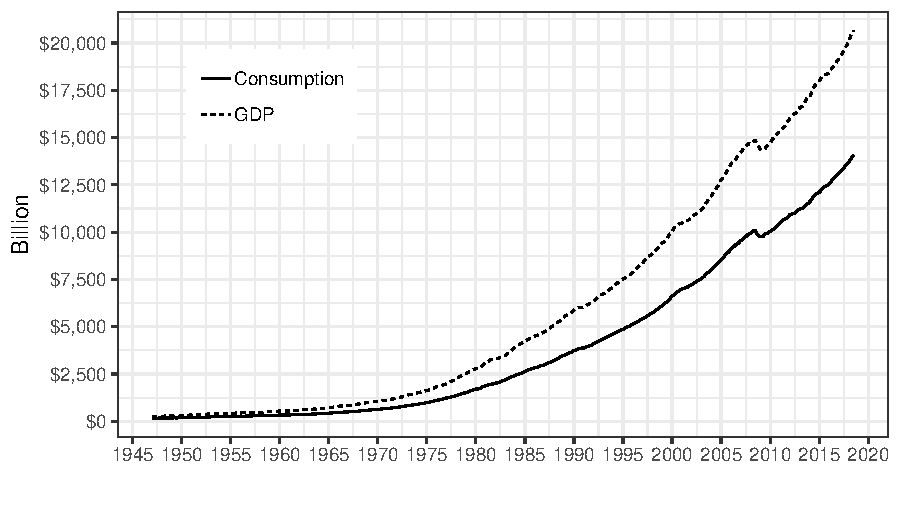
\includegraphics[width=1\linewidth]{ucla-102-fall2018_files/figure-latex/gdp-cons-1} 

}

\caption{\textsc{US GDP from NIPA (BEA)}.}\label{fig:gdp-cons}
\end{figure}

To get a better of sense of how big consumption is as a fraction to GDP
(although you may eyeball it on this picture), we might plot consumption
as a function of GDP, which is what I do on Figure
\ref{fig:consumption}. You can see that Personal Consumption
Expenditures are approximately \textbf{60 to 70 \% of GDP}. You can also
see that it has been rising since the end of the sixties. We will
discuss that.




\begin{figure}

{\centering 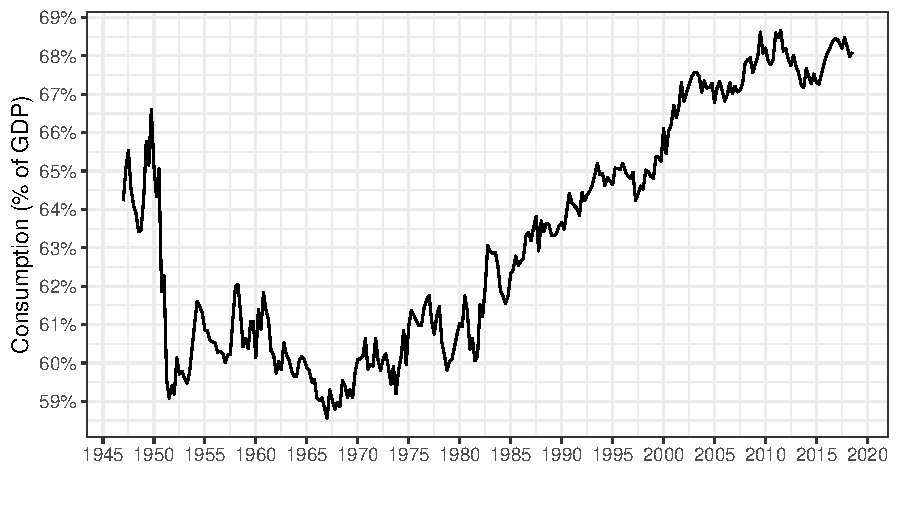
\includegraphics[width=1\linewidth]{ucla-102-fall2018_files/figure-latex/consumption-1} 

}

\caption{\textsc{Consumption as a share of GDP from NIPA
(BEA)}.}\label{fig:consumption}
\end{figure}

Personal Consumption Expenditures are divided up into:

\begin{itemize}
\tightlist
\item
  Durable Goods (more than 3 years of durability): e.g.~cars.
\item
  Non-durable Goods (less than 3 years of durability).
\item
  Services.
\end{itemize}

Services have become more important than Goods in total consumption
since the 1970s, as Figure \ref{fig:goods-vs-services} shows.




\begin{figure}

{\centering 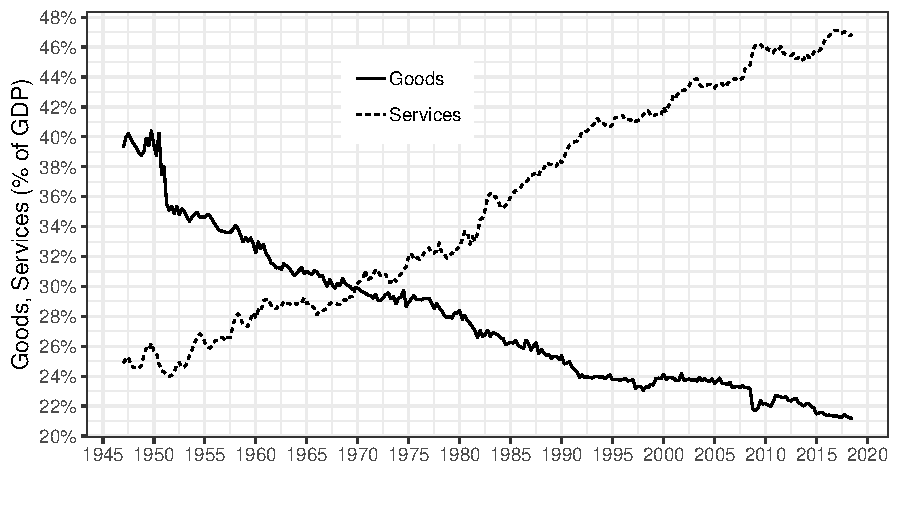
\includegraphics[width=1\linewidth]{ucla-102-fall2018_files/figure-latex/goods-vs-services-1} 

}

\caption{\textsc{Goods and Services Consumption as
a share of GDP from NIPA (BEA)}.}\label{fig:goods-vs-services}
\end{figure}

\hypertarget{inv}{\subsection{Investment (I)}\label{inv}}

Investment has two components:

\begin{itemize}
\tightlist
\item
  \textbf{non residential investment} is the purchase of new capital
  goods by firms: structures, new plants.
\item
  \textbf{residential investment} is the purchase of new houses.
\end{itemize}

Gross private domestic investment is approximately \textbf{15 to 20 \%
of GDP}, as you can see on Figure \ref{fig:inv}. It is also very
volatile over the cycle.



\begin{figure}

{\centering 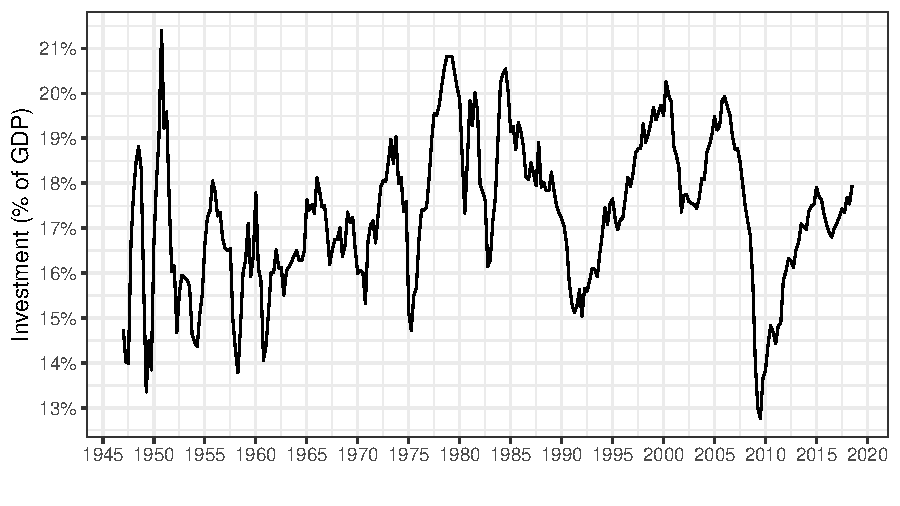
\includegraphics[width=1\linewidth]{ucla-102-fall2018_files/figure-latex/inv-1} 

}

\caption{\textsc{Investment as a share of GDP from NIPA (BEA)}.}\label{fig:inv}
\end{figure}

\hypertarget{gov}{\subsection{Government Purchases (G)}\label{gov}}

Government purchases are composed of purchases of goods by the
government plus the compensation of government employees. Overall, they
comprise about approximately 20\% of GDP, as can be seen on Figure
\ref{fig:g-purchases}. Note however that they do not include transfers
from the government of interest payments on government debt.




\begin{figure}

{\centering 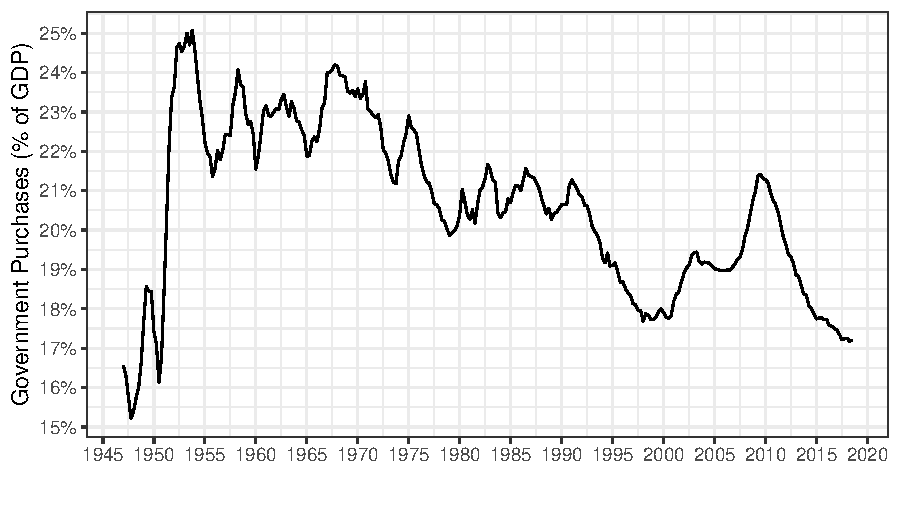
\includegraphics[width=1\linewidth]{ucla-102-fall2018_files/figure-latex/g-purchases-1} 

}

\caption{\textsc{Government Purchases as a share of GDP
from NIPA (BEA)}.}\label{fig:g-purchases}
\end{figure}

\hypertarget{net-exports}{\subsection{Net Exports
(NX)}\label{net-exports}}

Net exports of goods and services are approximately \textbf{-2 to -6 \%
of GDP}, at least in the modern period (and in the United States), as
you can see on Figure \ref{fig:net-exports}.




\begin{figure}

{\centering 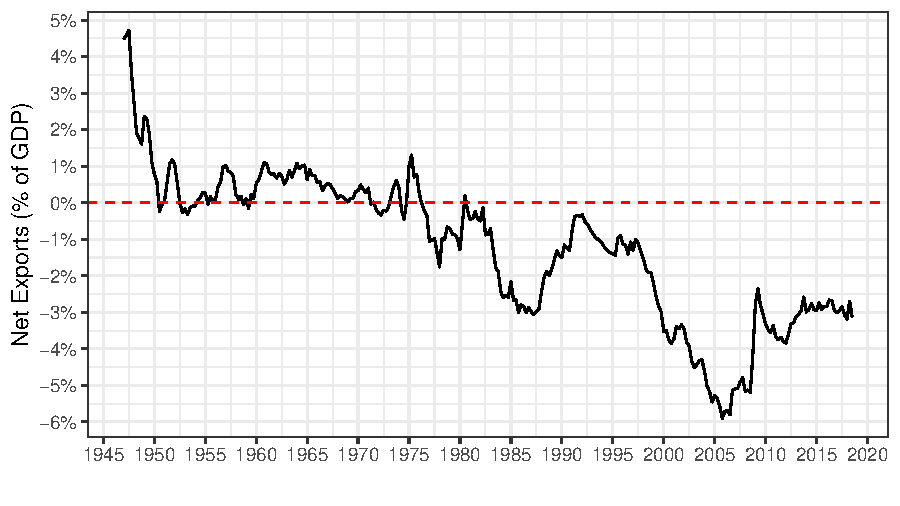
\includegraphics[width=1\linewidth]{ucla-102-fall2018_files/figure-latex/net-exports-1} 

}

\caption{\textsc{Net Exports as a share of GDP from NIPA
(BEA)}.}\label{fig:net-exports}
\end{figure}

\hypertarget{gdp-income}{\section{The Income Approach to
GDP}\label{gdp-income}}

\subsection{Cobb-Douglas Production
function}\label{cobb-douglas-production-function}

In order to organize our thinking, let's write out a Cobb-Douglas
production function, defined as:
\[Y_t = A_t K_t^{\alpha} L_t^{1-\alpha},\] where \(\alpha\) is a number
between \(0\) and \(1\). We will see later that this \(\alpha\) is
related to the share of capital versus labor in value added. In
practice, you should think of \(\alpha\) as close to \(1/3\). Again, we
shall explain why at the end of this lecture.

To proceed further, it is useful to think of a firm which would choose
the amount of labor it uses \(L_t\) as well as the amount of capital it
uses \(K_t\) in order to maximize its profits:\footnote{You may be
  asking yourself what this firm is. We are looking at aggregates here,
  and there sure isn't just one firm in the economy. However, if all
  firms were identical, because of constant return to scale, the
  ``representative'' firm aggregating the decisions of all individual
  firms would seem to be solving that problem.}
\[\max_{K_t, L_t} \quad A_t K_t^{\alpha} L_t^{1-\alpha} - R_t K_t - w_t L_t,\]

In this expression, \(R_t\) is the \textbf{rental rate} of capital, also
called the \textbf{gross return} to capital. This represents how much it
costs to rent one unit of capital. This cost actually has two
components:

\begin{enumerate}
\def\labelenumi{\arabic{enumi}.}
\item
  It includes a conventional interest rate \(r_t\), which is the cost of
  borrowing money to invest in capital. You should think of this as the
  real interest rate which is charged by a bank to borrow money.
\item
  It also includes a depreciation rate \(\delta\), which accounts for
  the wear and tear of the capital stock, implying that its value drops
  over time. If capital is bought, then the resale price for each unit
  of capital is lower by a fraction \(\delta\), which is a cost to the
  investor. If capital is rented, then capital needs to be given back to
  the owner in its original state.
\end{enumerate}

We have that the rental rate or gross return is equal to the net return
plus the depreciation rate: \[\boxed{R_t = r_t + \delta}.\] From Econ
11, it should be clear that a way to solve this problem is to set the
derivative of the profit function equal to \(0\) with respect to \(K_t\)
and \(L_t\):

\begin{itemize}
\tightlist
\item
  Differentiating with respect to \(K_t\) implies: \[
  \begin{aligned}
  \alpha A_t K_t^{\alpha-1} L_t^{1-\alpha} - R_t = 0 \quad \Rightarrow \quad \boxed{R_t = \alpha A_t K_t^{\alpha-1} L_t^{1-\alpha}}.
  \end{aligned}
  \]
\item
  Differentiating with respect to \(L_t\) implies:
  \[(1-\alpha) A_t K_t^{\alpha} L_t^{-\alpha} - w_t = 0 \quad \Rightarrow \quad \boxed{w_t = (1-\alpha) A_t K_t^{\alpha} L_t^{-\alpha}}.\]
\end{itemize}

Note that an alternative, and more direct way to get at that same
result, would be to use Econ 11 directly, and write that the marginal
products have to be equal to prices:

\begin{itemize}
\tightlist
\item
  The \textbf{rental rate of capital} \(R_t\) is the marginal product of
  capital. The marginal product of capital is how much more output is
  obtained when the capital stock is increased by one unit, which is
  just the derivative of output with respect to capital
  \(\partial Y_t / \partial K_t\): \[
  \begin{aligned}
  R_t&=\frac{\partial Y_t}{\partial K_t}\\
  &= \frac{\partial \left(A_t K_t^{\alpha} L_t^{1-\alpha}\right)}{\partial K_t}\\
  R_t &= \alpha A_t K_t^{\alpha-1} L_t^{1-\alpha}
  \end{aligned}
  \]
\item
  The \textbf{wage} \(w_t\) is the marginal product of labor. The
  marginal product of labor is how much more output is obtained when the
  quantity of labor is increased by one unit, which is just the
  derivative of output with respect to labor
  \(\partial Y_t / \partial L_t\): \[
  \begin{aligned}
  w_t &=\frac{\partial Y_t}{\partial L_t}\\
  &= \frac{\partial \left(A_t K_t^{\alpha} L_t^{1-\alpha}\right)}{\partial L_t}\\
  w_t &= (1-\alpha) A_t K_t^{\alpha} L_t^{-\alpha}
  \end{aligned}
  \]
\end{itemize}

The total capital income \(R_t K_t\) is a fraction \(\alpha\) of output
\(Y_t\): \[
\begin{aligned}
R_t K_t &= \alpha A_t K_t^{\alpha-1} L_t^{1-\alpha} \cdot K_t \\
&= \alpha A_t K_t^{\alpha} L_t^{1-\alpha}\\
R_t K_t &= \alpha Y_t.
\end{aligned}
\] This implies that the share of capital income in output (or
equivalently, value added) is: \[\boxed{\frac{R_t K_t}{Y_t}=\alpha}.\]

The total wage bill \(w_t L_t\) is a fraction \(1-\alpha\) of output
\(Y_t\): \[
\begin{aligned}
w_t L_t &= (1-\alpha) A_t K_t^{\alpha} L_t^{-\alpha} \cdot L_t \\
&= (1-\alpha) A_t K_t^{\alpha} L_t^{1-\alpha}\\
w_t L_t &= (1-\alpha) Y_t
\end{aligned}
\] The share of labor income in output \(w_t L_t/Y_t\) (or equivalently,
value added) is: \[\boxed{\frac{w_t L_t}{Y_t}=1-\alpha}.\]

Note that capital income plus labor income equals total output:
\[R_t K_t + w_t L_t = Y_t.\] Another way to say the same thing is that
the share of capital income in output and that of labor income in output
add up to one: \[\boxed{\frac{R_t K_t}{Y_t} + \frac{w_t L_t}{Y_t}=1}.\]

\subsection{The Income Side in the
Data}\label{the-income-side-in-the-data}

In practice, how much goes to the compensation of employees (labor
income), and how much goes to the returns to capital (capital income)?
The answer is that it goes approximately for 1/3 to capital and for 2/3
to labor. In turn, this implies that we will, in numerical applications
of our theories, often assume that: \[\alpha = \frac{1}{3}\] The
calculations for these are less straightforward than for computing the
share of consumption, investment, as we did above. The reason is that in
practice, the division between labor and capital is not as clear cut in
the national accounts as one might hope: for example, someone who owns
her/his own business reports most of her/his income in the form of
capital income, even when a large part of it is actually labor income,
so that compensation of employees is (vastly) understated. Figure
\ref{fig:comp-emp} shows which results are obtained using this
understated measure. It needs to be adjusted upwards by about 10\% of
GDP, for the reasons mentioned above.




\begin{figure}

{\centering 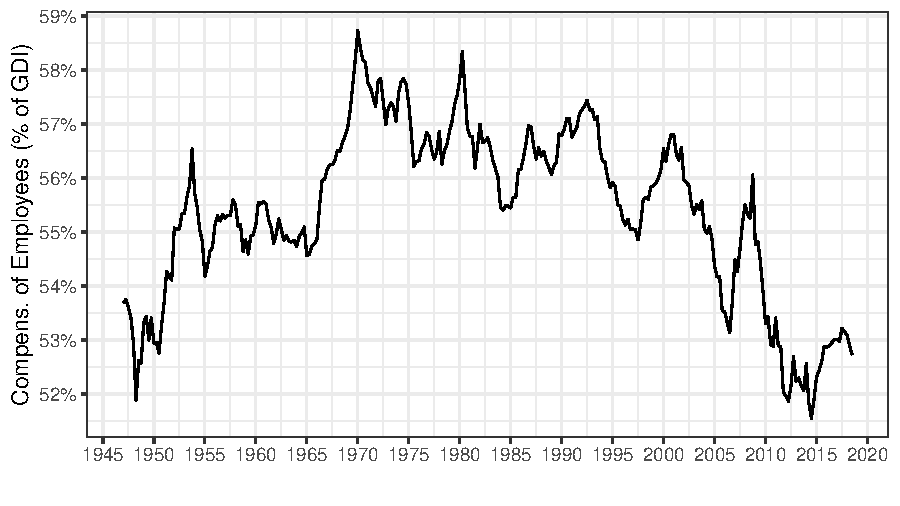
\includegraphics[width=1\linewidth]{ucla-102-fall2018_files/figure-latex/comp-emp-1} 

}

\caption{\textsc{Compensation of Employees as a share of GDP
from NIPA (BEA)}.}\label{fig:comp-emp}
\end{figure}

For our purposes, we only need to remember that the share of
compensation of employees is approximately 2/3 of value added:
\[1-\alpha \approx \frac{2}{3} \quad \Rightarrow \quad \boxed{\alpha \approx \frac{1}{3}}.\]

Therefore, we will very often work with a Cobb-Douglas production
function where \(\alpha=1/3\), implying that production is given by:
\[Y_t = A_t K_t^{1/3} L_t^{2/3}.\]
\protect\hyperlink{lecture-solow}{Lecture 2} will walk you through the
Solow growth model, where we shall make heavy use of that Cobb-Douglas
production function.

\section*{Readings - To go further}\label{readings---to-go-further}
\addcontentsline{toc}{section}{Readings - To go further}

\href{https://hbr.org/2012/01/the-economics-of-well-being}{The Economics
of Well Being, \emph{Harvard Business Review}.}

\href{https://search.proquest.com/hnpnewyorktimes/docview/1030670685/A9EF0C9A254D4699PQ/1?accountid=14512}{G.D.P.
R.I.P., \emph{The New York Times}, August 9, 2009.}

(Gated)
\href{https://www.economist.com/news/finance-and-economics/21677223-new-study-shows-money-can-buy-you-happinessbut-only-fleetingly-others}{Keeping
up with the Karumes, \emph{The Economist}, October 29, 2015.}

(More Difficult Read)
\href{https://doi.org/10.1257/089533005774357833}{Abraham, Katharine G.
``Distinguished Lecture on Economics in Government-What We Don't Know
Could Hurt Us: Some Reflections on the Measurement of Economic
Activity.'' Journal of Economic Perspectives 19, no. 3 (September 2005):
3--18.}

\hypertarget{solow}{\chapter{The Solow Growth Model}\label{solow}}

The \protect\hyperlink{general-production-f}{first part of this lecture}
considers the case of a Solow growth model with a general, constant
returns to scale, production function. The
\protect\hyperlink{cobb}{second part of the lecture} looks at a special
case of the Solow growth model for a case of a Cobb-Douglas production
function.

\hypertarget{general-production-f}{\section{General Production
Function}\label{general-production-f}}

\subsection{Assumptions}\label{assumptions}

Robert Solow, 1987 Nobel Memorial Prize in Economic Sciences, starts
from a general production function, giving at any point in time output
\(Y_t\) as a function of inputs, capital \(K_t\) and labor \(L_t\):
\[Y_t=F\left(K_t,L_t\right).\] A very important assumption is also
\textbf{constant returns to scale} with respect to capital and labor, so
that for any scaling factor \(a\): \[F(aK_t, aL_t) = aF(K_t, L_t).\]

For simplicity, we shall assume from now on that the quantity of labor
is fixed with \(L_t=L\), so that the production function becomes
\(Y_t=F(K_t, L)\). Because of constant returns to scale with respect to
capital and labor (and setting \(a=1/L\) in the previous expression), we
have:
\[\frac{Y_t}{L}=F\left(\frac{K_t}{L},1\right)=f\left(\frac{K_t}{L}\right)\]
where \(f\) is defined as a function of \(F\) such that:
\[f(x)\equiv F(x,1).\]

An example of such a production function is the Cobb-Douglas production
function, which we started studying in
\protect\hyperlink{intro-cobb}{Lecture 1}, and which we look at in the
\protect\hyperlink{cobb}{next section}.

Robert Solow, in his 1956 contribution, abstracts from public saving, so
that \textbf{total saving} at time \(t\) equals \textbf{private saving}
at time \(t\), and both are denoted \(S_{t}\), which also equals
investment \(I_{t}\) at time \(t\) : \[S_{t}=I_{t}.\]

Saving is assumed to be a constant fraction \(s\) of output \(Y_{t}\),
and therefore: \[S_{t}=sY_{t}.\]

This constant saving rate my seem a bit ad-hoc; it is. We will
investigate more in detail the determinants of saving and consumption
behavior in the next lectures. Depreciation of capital is given by a
share \(\delta\) (think for example that 8\% of the capital stock
depreciates each period; the rate of depreciation is much lower for
structures, and much higher for computers). The capital stock evolves
according to: \[K_{t+1}=\left(1-\delta\right)K_{t}+I_{t}\]

\subsection{Solution}\label{solution}

Replace investment in the previous equation and divide both sides by
\(L\):
\[\frac{K_{t+1}}{L} =\left(1-\delta\right)\frac{K_{t}}{L}+s\frac{Y_{t}}{L}\quad\Rightarrow\quad\boxed{\frac{K_{t+1}}{L}-\frac{K_{t}}{L}=s\frac{Y_{t}}{L}-\delta\frac{K_{t}}{L}}\]

The change in the capital stock per person from \(t\) to \(t+1\) has two
components: investment (or saving) and depreciation:

\[\underbrace{\frac{K_{t+1}}{L}-\frac{K_{t}}{L}}_{\text{Change in capital }}=\underbrace{sf\left(\frac{K_{t}}{L}\right)}_{\text{Investment}}-\underbrace{\delta\frac{K_{t}}{L}}_{\text{Depreciation}}.\]

The steady state level of the capital stock \(K^{*}\) is such that
\(K_{t+1}=K_{t}=K^{*}\), and it therefore satisfies:
\[\boxed{sf\left(\frac{K^{*}}{L}\right)=\delta\frac{K^{*}}{L}}\]

Note that without further specifying \(f(.)\), we can't say much more
about the value of \(K^{*}/L\), we just know it satisfies this implicit
equation. The steady-state value of output per worker \(Y^{*}/L\), as a
function of \(K^{*}/L\) is given by:
\[\frac{Y^{*}}{L}=f\left(\frac{K^{*}}{L}\right)\]

\subsection{Three cases}\label{three-cases}

There are 3 cases:

\begin{enumerate}
\def\labelenumi{\arabic{enumi}.}
\item
  If capital per worker is relatively low, that is \(K_{t}/L<K^{*}/L\),
  then investment per worker is larger than depreciation per worker, and
  therefore from the above equation, capital per worker increases:
  \[\frac{K_{t+1}}{L}>\frac{K_{t}}{L}\]
\item
  If capital per worker is exactly equal to steady state capital per
  worker, that is \(K_{t}/L=K^{*}/L\), then investment per worker is
  equal to depreciation per worker, and therefore from the above
  equation, capital per worker stays constant:
  \[\frac{K_{t+1}}{L}=\frac{K_{t}}{L}=\frac{K^{*}}{L}\]
\item
  If capital per worker is relatively high, that is \(K_{t}/L>K^{*}/L\),
  then depreciation per worker is larger than investment per worker, and
  therefore, capital per worker declines:
  \[\frac{K_{t+1}}{L}<\frac{K_{t}}{L}.\]
\end{enumerate}

\hypertarget{cobb}{\section{Cobb-Douglas production
function}\label{cobb}}

\subsection{Solving for the model}\label{solving-for-the-model}

Assume now that the production function is a Cobb-Douglas production
function, so that:\\
\[F(K,L)=K^{\alpha}L^{1-\alpha}\] As we saw during
\protect\hyperlink{intro-cobb}{lecture 1}, \(\alpha\) should be thought
of as roughly equal to \(\alpha = 1/3\). This implies then that function
\(f\) defined above is such that: \[f(x)=x^{\alpha}\]

The law of motion for capital is given by:\\
\[\frac{K_{t+1}}{L}=\frac{K_{t}}{L}+s\left(\frac{K_{t}}{L}\right)^{\alpha}-\delta\frac{K_{t}}{L}.\]

Given \(L\), \(K_{0}\), \(\alpha\), \(s\), \(\delta\), we are able to
calculate \(K_{1}\), \(K_{2}\), \ldots{}, as well as \(K_{t}\) for any
\(t\), by calculating the quantities of capital successively from the
formula above.

If you do so, you will notice that \(K_{t}\) converges to a steady state
value \(K^{*}\). However, you do not need to perform an infinity of
operations to get at this \(K^{*}\). Instead, you can see that capital
per worker in steady-state \(K^{*}/L\) solves:

\[s\left(\frac{K^{*}}{L}\right)^{\alpha}=\delta\frac{K^{*}}{L}\quad\Rightarrow\quad \boxed{\frac{K^{*}}{L}=\left(\frac{s}{\delta}\right)^{\frac{1}{1-\alpha}}}\]
What was an implicit equation in the
\protect\hyperlink{general-production-f}{previous section} can now be
solved for explicitely. The steady-state level of output per worker is
then:
\[\frac{Y^{*}}{L}=\left(\frac{s}{\delta}\right)^{\frac{\alpha}{1-\alpha}}\]

We are finally able to compute the capital to output ratio
\(K^{*}/Y^{*}\) from the Solow growth model: \[
\begin{aligned}
\frac{K^{*}}{Y^{*}}&=\frac{K^{*}/L}{Y^{*}/L}\\
&=\left(\frac{s}{\delta}\right)^{\frac{1}{1-\alpha}}  \left(\frac{s}{\delta}\right)^{-\frac{\alpha}{1-\alpha}} \\
\frac{K^{*}}{Y^{*}}&= \frac{s}{\delta}.
\end{aligned}
\] Alternatively, you may obtain this expression much more simply by
equating saving \(sY^{*}\) to investment \(\delta K^{*}\) in the steady
state:
\[sY^{*} = \delta K^{*} \quad \Rightarrow \quad \boxed{\frac{K^{*}}{Y^{*}} = \frac{s}{\delta}}.\]

\subsection{Golden Rule}\label{golden-rule}

Most economists believe that policymakers should not care so much about
GDP per person, but rather about consumption per person (however, some
people hold a different view -- we shall talk about that later). The
intuition is simple: if an economy was to produce many goods which were
only used for investment purposes (which would be the case if
\(s = 1\)), then people in this economy would be starving, even though
it was actually producing a lot. Investment, ultimately, should serve to
increase future consumption.

The \textbf{Golden Rule level of capital accumulation} is such that the
level of steady-state consumption per capita is maximized. The
steady-state consumption per capita is given by: \[
\begin{aligned}
\frac{C^{*}}{L}&=(1-s)\frac{Y^{*}}{L}\\
&=(1-s)\left(\frac{s}{\delta}\right)^{\frac{\alpha}{1-\alpha}}\\
\frac{C^{*}}{L}&=\frac{(1-s)s^{\frac{\alpha}{1-\alpha}}}{\delta^{\frac{\alpha}{1-\alpha}}}
\end{aligned}
\]

Maximizing this steady state consumption with respect to the saving rate
\(s\) consists in finding the maximum of that function with respect to
\(s\):
\[\frac{d\left(C^{*}/L\right)}{ds}=0\quad\Rightarrow\quad\frac{d\left[(1-s)s^{\frac{\alpha}{1-\alpha}}\right]}{ds}=0\]

Note that the \(1/\delta^{\alpha/(1-\alpha)}\) is just a constant which
does not change anything to the maximization. If you are not convinced,
then you may also compute the derivative with respect to the whole
\(C^{*}/L\) expression. This gives: \[
\begin{aligned}
&-s^{\frac{\alpha}{1-\alpha}}+\frac{\alpha}{1-\alpha}(1-s)s^{\frac{\alpha}{1-\alpha}-1} =0 \quad \Rightarrow\quad\frac{\alpha}{1-\alpha}\frac{1-s}{s}=1\\
&\quad \quad \Rightarrow\quad\alpha-\alpha s=s-\alpha s \quad\Rightarrow\quad\boxed{s=\alpha}.
\end{aligned}
\] Therefore, the saving rate corresponding to the Golden Rule level of
capital accumulation is equal to \(\alpha\) (again, taking \(\alpha\) to
be equal to roughly 1/3, this would suggest that an economy would
optimally need to save about a third of its production every year).

The Golden Rule level of capital accumulation is then such that capital
at the steady-state is given as a function of the exogenous parameters
by:
\[\frac{K^{*}}{L}=\left(\frac{\alpha}{\delta}\right)^{\frac{1}{1-\alpha}}\quad\Rightarrow\quad K^{*}=L\left(\frac{\alpha}{\delta}\right)^{\frac{1}{1-\alpha}}\]

The level of GDP corresponding to this Golden rule level is:
\[Y^{*}=L\left(\frac{\alpha}{\delta}\right)^{\frac{\alpha}{1-\alpha}}.\]

\section{Some Data}\label{some-data}

Figure \ref{fig:gross-sav-inv} plots gross saving and investment in the
United States from the World Development Indicators put together by the
World Bank. Figure \ref{fig:net-sav-inv} plots net saving and gross
saving for the U.S.: net saving (gross saving net of depreciatin) is
slightly higher than 0, but not by much. Figure \ref{fig:inv-gdp} plots
investment as a \% of GDP on a map of the world, while figure
\ref{fig:sav-gdp} plots gross saving as a \% of GDP.




\begin{figure}

{\centering 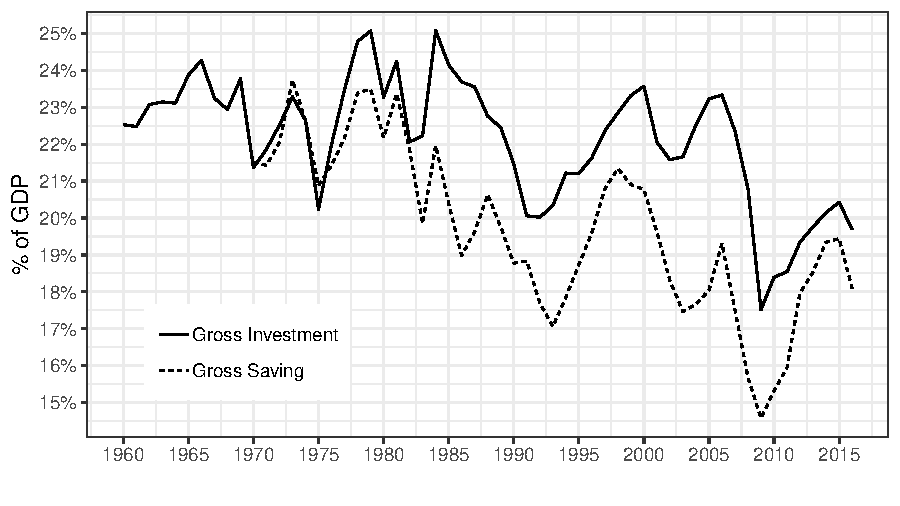
\includegraphics[width=1\linewidth]{ucla-102-fall2018_files/figure-latex/gross-sav-inv-1} 

}

\caption{\textsc{Gross Savings and Investment in the
U.S. (WDI)}.}\label{fig:gross-sav-inv}
\end{figure}



\begin{figure}

{\centering 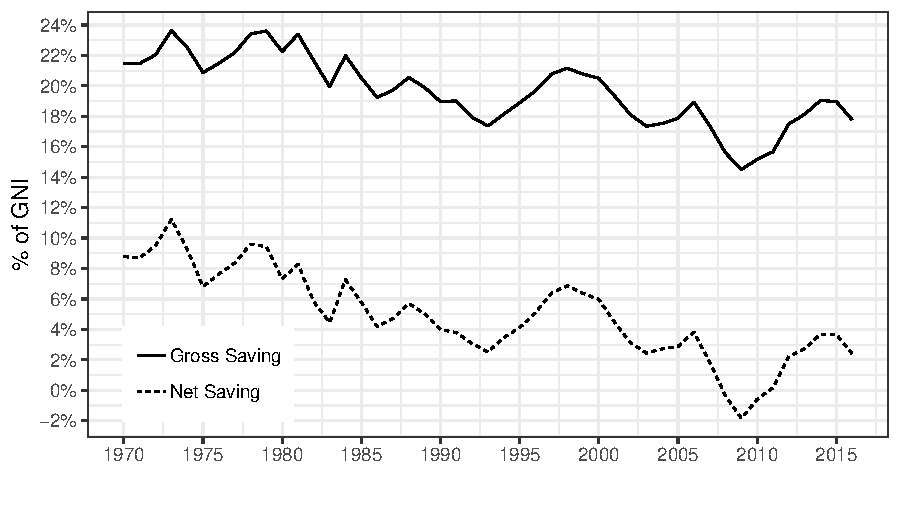
\includegraphics[width=1\linewidth]{ucla-102-fall2018_files/figure-latex/net-sav-inv-1} 

}

\caption{\textsc{Net Savings and Gross savings (WDI)}.}\label{fig:net-sav-inv}
\end{figure}



\begin{figure}

{\centering 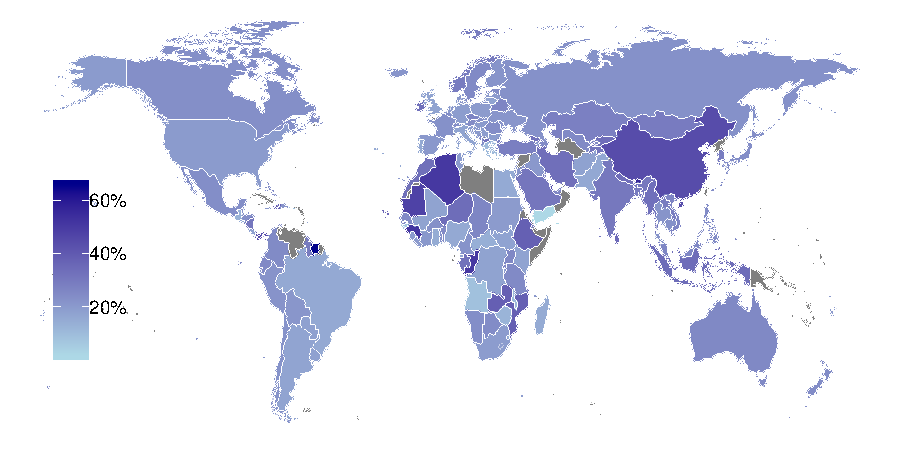
\includegraphics[width=1\linewidth]{ucla-102-fall2018_files/figure-latex/inv-gdp-1} 

}

\caption{\textsc{Investment (\% of GDP), 2016}.}\label{fig:inv-gdp}
\end{figure}



\begin{figure}

{\centering 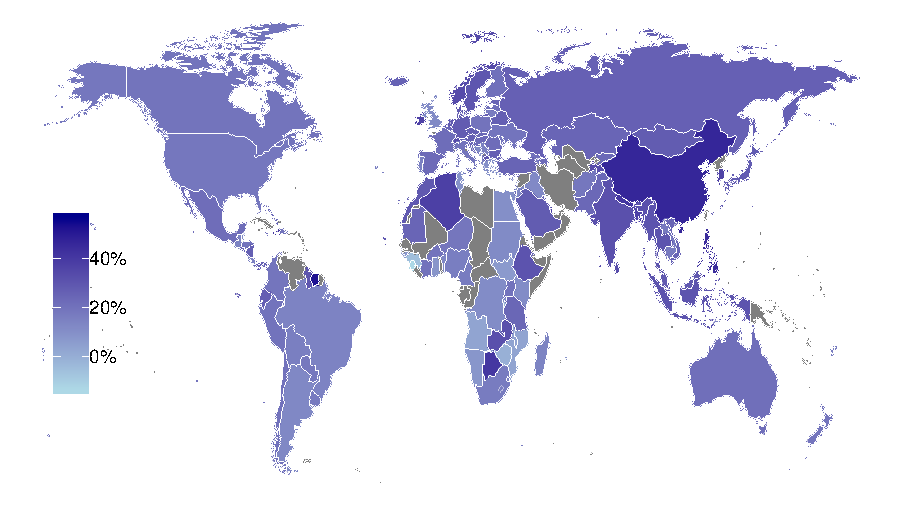
\includegraphics[width=1\linewidth]{ucla-102-fall2018_files/figure-latex/sav-gdp-1} 

}

\caption{\textsc{Gross Saving (\% of GDP), 2016}.}\label{fig:sav-gdp}
\end{figure}

\section*{Readings - To go further}\label{readings---to-go-further-1}
\addcontentsline{toc}{section}{Readings - To go further}

\href{https://www.wsj.com/articles/humans-1-robots-0-1381098947?tesla=y}{Humans
1, Robots 0, \emph{Wall Street Journal}, October 6, 2013.}

(Gated)
\href{https://www.economist.com/finance-and-economics/2018/04/12/economists-understand-little-about-the-causes-of-growth}{Economists
understand little about the causes of growth, \emph{The Economist},
April 12, 2018.}

\hypertarget{two-period}{\chapter{Two Period Consumption
Problem}\label{two-period}}

Consumption and saving are perhaps the most important and controversial
issues in macroeconomics. In the Solow growth model, saving was a
constant fraction \(s\) of GDP, by assumption. We now build on
\emph{Economics 11} (the one where you learn consumer optimization with
Lagrangians and all that), in order to derive saving behavior from
microeconomic principles. In other words, we work to make saving
``endogenous'' (that is, explained by the model), while it was
previously taken as exogenous (that is, assumed in the model).

Although this discussion may appear somewhat abstract at first, these
calculations are the basis of some of the most important controversies
in macroeconomics, which we shall come to in the next lectures.

\section{The Two-Period Consumption
Problem}\label{the-two-period-consumption-problem}

\subsection{Assumptions}\label{assumptions-1}

There are two periods, \(t=0\) (think of this as ``today'') and \(t=1\)
(think of this as ``tomorrow''). The consumer values consumption \(c_0\)
in period \(0\) and \(c_1\) in period \(1\) according to the following
utility function:

\[U(c_{0},c_{1})=u(c_{0})+\beta u(c_{1}).\]

where \(u(.)\) is an increasing and concave function, and
\(\beta \leq 1\). \(\beta\) captures that people typically have a
preference for the present. (they are \textbf{present-biased})

Assume that agents earn (labor) income \(y_{0}\) in period \(0\), and
(labor) income \(y_{1}\) in period \(1\). They also are born with some
financial wealth \(f_{0}\) now, and have financial wealth \(f_{1}\) in
period 1, which they consume entirely because this is the last period.
(there is no point keeping more money for after period 1, because there
is no future at that point) The amount that agents save in this economy
is thus \(f_{1}-f_{0}\), and the amount of their accumulated savings is
the savings they already had plus what they decided to accumulate, so
that \(f_{0}+(f_{1}-f_{0})=f_{1}.\)

Therefore, consumption in period \(0\) is given by:

\[c_{0} =y_{0}-(f_{1}-f_{0})\]

The second period consumption \((t=1)\) is given by income plus the
return to (accumulated !) savings:

\[c_{1} =y_{1}+(1+r)f_{1}.\]

\subsection{Constrained Optimization
Problem}\label{constrained-optimization-problem}

Here, we show that the previous problem can actually be written as a
maximization problem, subject to a budget constraint.

\textbf{Intertemporal budget constraint.} Rewriting \(f_{1}\) from this
second equation: \(f_{1}=(c_{1}-y_{1})/(1+r)\), and plugging into the
first,

\[c_{0}=y_{0}-\left(\frac{c_{1}-y_{1}}{1+r}-f_{0}\right).\] Rearranging,
total wealth is then the sum of financial wealth \(f_0\) and of the
present discounted value of human wealth:

\[c_{0}+\frac{c_{1}}{1+r}=\overbrace{f_{0}+\underbrace{y_{0}+\frac{y_{1}}{1+r}}_{\text{human wealth}}}^{\text{total wealth}}.\]

The intertemporal budget constraint says that the present discounted
value of consumption is equal to total wealth.

\textbf{Optimization.} The problem of the consumer is then simply that
of maximizing utility under his budget constraint:

\[
\begin{aligned} 
\max_{c_{0},c_{1}} & \quad u(c_{0})+\beta u(c_{1}) \\
& \text{s.t.} \quad c_{0}+\frac{c_{1}}{1+r}=f_{0}+y_{0}+\frac{y_{1}}{1+r}.
\end{aligned}
\]

\subsection{4 methods}\label{methods}

You may solve this optimization in four different ways:

\begin{enumerate}
\def\labelenumi{\arabic{enumi}.}
\item
  Apply the well known ratio of marginal utilities formula from Econ 11.
  Let us rewrite this optimization problem as follows: \[
  \begin{aligned} 
  \max_{c_{0},c_{1}} & \quad u(c_{0})+\beta u(c_{1}) \\
  & \text{s.t.} \quad p_0c_{0}+p_1 c_1=B.
  \end{aligned}
  \] where we have defined the price of consumption in period \(0\) by:
  \[p_0 \equiv 1,\] the price of consumption in period \(1\) by:
  \[p_1 \equiv \frac{1}{1+r},\] and finally the budget \(B\) by the
  present discounted value of lifetime resources:
  \[B \equiv f_{0}+y_{0}+\frac{y_{1}}{1+r}.\] Note that the relative
  price of consumption in period \(1\) relative to period \(0\) is given
  by \(1/(1+r)\): when the interest rate becomes higher, consuming in
  period \(1\) becomes relatively cheaper, or consuming in period \(0\)
  becomes more expensive (it's really expensive to consume now rather
  than later if the bank is offering me a really high interest rate).
  Thus, applying the formula from Econ 11 allows to say that the
  marginal rate of substitution between consumption in period \(1\)
  \(c_1\) and consumption in period \(0\) \(c_0\) - the ratio of
  marginal utilities - is equal to the ratio of prices:
  \[\frac{\partial U / \partial c_1}{\partial U / \partial c_0} = \frac{p_1}{p_0}= \frac{1}{1+r} \quad\Rightarrow\quad \boxed{\frac{\beta u'(c_{1})}{u'(c_{0})}=\frac{1}{1+r}}.\]
\item
  Apply the following intuitive economic argument. The marginal utility
  from consuming in period \(1\) is \(\beta u'(c_{1})\). The marginal
  utility from consuming in period \(0\) is \(u'(c_{0})\). By putting
  one unit of consumption in the bank, one forgoes \(1\) unit of
  consumption in period \(0\) to get \(1+r\) units of consumption in
  period \(1\). The two have to be equal, if one is optimizing. If
  consuming more in period \(0\) gives a higher marginal utility, or
  \(u'(c_{0})>(1+r)\beta u'(c_{1})\), then one should consume more and
  save less. On the contrary, should \(u'(c_{0})<(1+r)\beta u'(c_{1})\),
  one should consume less and save more. Therefore, in equilibrium,
  these two options can only be equal:
  \[u'(c_{0})=(1+r)\beta u'(c_{1})\quad\Rightarrow\quad \boxed{\frac{\beta u'(c_{1})}{u'(c_{0})}=\frac{1}{1+r}}.\]
\item
  Replace \(c_{0}\) from the intertemporal budget constraint above and
  optimize with respect to \(c_{1}\):
  \[\max_{c_{1}}\quad u\left[\left(f_{0}+y_{0}+\frac{y_{1}}{1+r}\right)-\frac{c_{1}}{1+r}\right]+\beta u(c_{1}).\]
  Taking the derivative of this expression with respect to \(c_1\) leads
  to: \[
  \begin{aligned}
  &-\frac{1}{1+r} u'\left[\left(f_{0}+y_{0}+\frac{y_{1}}{1+r}\right)-\frac{c_{1}}{1+r}\right]+\beta u'(c_{1})=0\\
  &\quad\Rightarrow\quad-\frac{1}{1+r}u'(c_{0})+\beta u'(c_{1})=0\quad\Rightarrow\quad \boxed{\frac{\beta u'(c_{1})}{u'(c_{0})}=\frac{1}{1+r}}.
  \end{aligned}
  \] where the first substitution uses the intertemporal budget
  constraint which implies: \[
  \begin{aligned}
  \left(f_{0}+y_{0}+\frac{y_{1}}{1+r}\right)-\frac{c_{1}}{1+r}=c_0
  \end{aligned}
  \]
\item
  Alternatively, you may substitute \(c_{1}\) out and optimize with
  respect to \(c_{0}\): \[
  \begin{aligned}
  \max_{c_{0}}\quad u(c_{0})+\beta u\left[(1+r)\left(f_{0}+y_{0}+\frac{y_{1}}{1+r}\right)-(1+r)c_{0}\right].
  \end{aligned}
  \] Taking the derivative of this expression with respect to \(c_0\)
  leads to: \[
  \begin{aligned}
  &u'(c_{0})-\beta(1+r)u'\left[(1+r)\left(f_{0}+y_{0}+\frac{y_{1}}{1+r}\right)-(1+r)c_{0}\right]=0\\
  &\quad\Rightarrow\quad u'(c_{0})-\beta(1+r)u'(c_{1})=0\quad\Rightarrow\quad \boxed{\frac{\beta u'(c_{1})}{u'(c_{0})}=\frac{1}{1+r}}.
  \end{aligned}
  \] where the first substitution uses the intertemporal budget
  constraint which implies (pre-multiplying both sides by \(1+r\)): \[
  \begin{aligned}
  (1+r)\left(f_{0}+y_{0}+\frac{y_{1}}{1+r}\right)-(1+r)c_{0}=c_1
  \end{aligned}
  \]
\end{enumerate}

\section{Some examples}\label{some-examples}

\subsection{Log utility, no
discounting}\label{log-utility-no-discounting}

Log utility implies that \(u(c)\) is given by the natural logarithm.
Marginal utility is then just: \[u'(c)=\frac{1}{c},\]

Since \(\beta=1\), the above optimality condition (derived 4 times) can
be written as: \[
\begin{aligned}
& \frac{u'(c_{1})}{u'(c_{0})}=\frac{1}{1+r} \quad \Rightarrow \quad \frac{1/c_1}{1/c_0}=\frac{1}{1+r} \\
& \quad \Rightarrow \quad \frac{c_0}{c_1}=\frac{1}{1+r} \quad \Rightarrow \quad c_{0}=\frac{c_{1}}{1+r}
\end{aligned}
\] Substituting out \(c_{1}/(1+r)=c_0\) in the intertemporal budget
constraint allows to calculate consumption at time \(0\) \(c_0\): \[
\begin{aligned}
&c_{0}+\frac{c_{1}}{1+r}=f_{0}+y_{0}+\frac{y_{1}}{1+r}\\
&\quad \Rightarrow \quad c_{0}+c_0=f_{0}+y_{0}+\frac{y_{1}}{1+r}\\
&\quad \Rightarrow \quad c_{0}=\frac{1}{2}\left(f_{0}+y_{0}+\frac{y_{1}}{1+r}\right)
\end{aligned}
\] Finally, we may calculate \(c_1\): \[
\begin{aligned}
c_{1}&=(1+r)c_0=\frac{1+r}{2}\left(f_{0}+y_{0}+\frac{y_{1}}{1+r}\right).
\end{aligned}
\]

According to this expression, the \textbf{Marginal Propensity to Consume
(MPC)} out of current wealth \(f_{0}\) is given by \(1/2\). When \(f_0\)
rises to \(f_0+\Delta f_0\), the corresponding change in consumption is:
\[\Delta c_0 = \frac{1}{2}\Delta f_0.\] If we were to study a model with
more periods, say \(T\) periods, we would find that people Marginal
Propensity to Consume is approximately equal to \(1/T\), at least
according to this model. Whether such is actually the case, and people
are that rational, is a subject of fierce debate among macroeconomists,
and one that we will take up in the next lectures.

\subsection{Log utility, with
discounting}\label{log-utility-with-discounting}

Marginal utility is then \(u'(c)=1/c\), so that the optimality condition
gives: \[
\begin{aligned}
& \frac{\beta u'(c_{1})}{u'(c_{0})}=\frac{1}{1+r} \quad \Rightarrow \quad \frac{\beta/c_1}{1/c_0}=\frac{1}{1+r} \\
& \quad \Rightarrow \quad \frac{\beta c_0}{c_1}=\frac{1}{1+r} \quad \Rightarrow \quad \beta c_{0}=\frac{c_{1}}{1+r}
\end{aligned}
\] Substituting out \(c_{1}/(1+r)=\beta c_0\) in the intertemporal
budget constraint allows to calculate consumption at time \(0\) \(c_0\):
\[
\begin{aligned}
&c_{0}+\frac{c_{1}}{1+r}=f_{0}+y_{0}+\frac{y_{1}}{1+r}\\
&\quad \Rightarrow \quad c_{0}+\beta c_0=f_{0}+y_{0}+\frac{y_{1}}{1+r}\\
&\quad \Rightarrow \quad c_{0}=\frac{1}{1+\beta}\left(f_{0}+y_{0}+\frac{y_{1}}{1+r}\right)
\end{aligned}
\] Finally, we may calculate \(c_1\): \[
\begin{aligned}
c_{1}&=\beta (1+r)c_0=\frac{\beta(1+r)}{1+\beta}\left(f_{0}+y_{0}+\frac{y_{1}}{1+r}\right).
\end{aligned}
\]

Because people are more impatient in this case, they consume more, and
their Marginal Propensity to Consume (MPC) is \textbf{higher} with
\(\beta<1\): \[\Delta c_0 = \frac{1}{1+\beta}\Delta f_0.\]

Note that the solution with no discounting corresponds to that with
discounting when \(\beta=1\), which was expected.

\section{Generalization}\label{generalization}

Assume that an individual receives wage \(w\) in period \(0\), and that
this wage is expected to grow at rate \(g\) in the next \(T\) years.
What is the present value of his human wealth, assuming that the
interest rate is given by \(R\)? The answer is that his human wealth
\(H\) is given as follows:

\[H =w+w\frac{1+g}{1+r}+w\left(\frac{1+g}{1+r}\right)^{2}+...+w\left(\frac{1+g}{1+r}\right)^{T-1}\]

\[H =w\frac{1-\left(\dfrac{1+g}{1+r}\right)^{T}}{1-\dfrac{1+g}{1+r}}\]

\hypertarget{olg}{\chapter{The Overlapping Generations
Model}\label{olg}}

In the Solow growth model, we assumed that saving was a constant
fraction of GDP. \protect\hyperlink{solow}{Lecture 2} has shown how to
use microeconomics, and optimization, in order to derive saving behavior
endogenously (that is, to explain it).

This section presents a very simple version of
\href{https://en.wikipedia.org/wiki/Peter_Diamond}{Peter Diamond}'s
\textbf{overlapping-generations model}, published in 1965 - if you would
like to read the original paper (you probably don't), it's
\href{https://www.jstor.org/stable/1809231}{here}.\footnote{Needless to
  say, you are not responsible for reading the original paper for the
  exam!} This model is used not just to give microfoundations to
\href{https://en.wikipedia.org/wiki/Robert_Solow}{Robert Solow}'s growth
model, but also to think about social security, public debt, an endeavor
which we will take up in the next lectures as well as in the problem
sets. During this lecture, I will present a very simplified version of
Peter Diamond's overlapping generations model.

\section{Assumptions}\label{assumptions-2}

\subsection{Time}\label{time}

We assume that people in this economy live only for \(2\) periods.
People are called ``young'' in the first period of their life, and
``old'' in the second. Thus, you should really think that the length of
a period is a generation (approximately 30 years). However, instead of
referring to these two periods as \(0\) and \(1\), I shall refer to them
as \(t\) and \(t+1\).

\subsection{Demographics}\label{demographics}

People from generation \(t\) are young in period \(t\), and old in
period \(t+1\). We denote their consumption when young by \(c_{t}^{y}\)
and their consumption when old by \(c_{t+1}^{o}\). In terms of
\protect\hyperlink{two-period}{Lecture 3}, you should really think of
\(c_{t}^{y}\) as \(c_{0}\), and of \(c_{t+1}^{o}\) as \(c_{1}\).

People work when young, and then receive a wage given by \(w_{t}\). They
retire when old, and then do not work. Their lifetime utility is
logarithmic with \(\beta=1\):

\[U=\log(c_{t}^{y})+\log(c_{t+1}^{o}).\]

Their intertemporal budget constraint is given by:

\[c_{t}^{y}+\frac{c_{t+1}^{o}}{1+r}=w_{t}.\]

There are always two generations living in period \(t\): the previous
period's young, born in period \(t-1\), now old, consuming the return
from their savings; and this period's young, newly born (in period
\(t\)).

\subsection{Production}\label{production}

For simplicity, we shall assume a Cobb-Douglas, constant returns to
scale, production function: \[Y_{t}=K_{t}^{\alpha}L_{t}^{1-\alpha}.\]

We assume that the labor force is constant and fixed to unity (this is
to avoid carrying \(L\) around everywhere - from
\protect\hyperlink{solow}{lecture 2}, you should now know that
everything can be expressed per capita, because of constant returns to
scale), and therefore:

\[L_{t}=L=1.\]

Again for simplicity, we shall assume that capital depreciates at rate
\(\delta=1=100\%\). (that is, capital fully depreciates each period -
this is not that unreasonable if you take one unit of time to represent
one generation, or about 30 years - remember that the depreciation rate
for one year was approximately equal to 2\% to 30\% depending on the
type of capital involved.)

\section{Solution}\label{solution-1}

\subsection{Saving}\label{saving}

Utility is logarithmic, so that the consumption of the young
\(c_{t}^{y}\) and consumption of the old \(c_{t+1}^{o}\) are given as a
function of the wage as follows (this is just an application of
\protect\hyperlink{two-period}{Lecture 3}):

\[c_{t}^{y}=\frac{w_{t}}{2}\qquad c_{t+1}^{o}=(1+r)\frac{w_{t}}{2}.\]

Indeed, if you want to think of this model as the two periods model of
\protect\hyperlink{two-period}{Lecture 3}, think that everything is as
if:

\[f_{0}=0,\qquad y_{0}=w_{t},\qquad y_{1}=0.\]

\subsection{Capital accumulation}\label{capital-accumulation}

Saving (and savings) is equal to investment, and therefore we have that:
\[S_t = I_t = w_{t}-c_{t}^{y}=\frac{w_{t}}{2}.\]

The major difference with the Solow model is that saving is here
endogenous, and coming from agents' optimizing choices. In the Solow
model in contrast, saving was taken as exogenous and equal to a fraction
\(s\).

The wage paid by employers, given that \(L=1\), is:
\[w_{t}=(1-\alpha)K_{t}^{\alpha}L^{-\alpha}=(1-\alpha)K_{t}^{\alpha} = (1-\alpha)Y_t.\]

Finally:
\[\Delta K_{t+1}=\frac{w_{t}}{2}-\delta K_{t} = \frac{1-\alpha}{2}Y_t-\delta K_t.\]

This is the capital accumulation equation (or law of motion for capital)
of the Solow model, with \(s = (1-\alpha)/2\). The new element here of
course is to get saving endogenously, from agents' optimal decisions.
Note that the value for the saving rate has an economic interpretation:
wages are only a fraction \(1-\alpha\) of output, from
\protect\hyperlink{intro-cobb}{lecture 1}. On the other hand, savers /
consumers want to smooth consumption and therefore want to save a half
of that. This is why a fraction \((1-\alpha)/2\) of output is saved.

\subsection{Numerical Application}\label{numerical-application}

Note that if \(\alpha=1/3\), then the saving rate is equal to
\(s = 1/3\), which happens to be (by coincdence) the Golden Rule level
of saving. This does not mean that the Golden Rule level is always
satisfied. This only happens by chance in this very stylized model. In
particular, saving is not just because of retirement, but also because
of precautionary behavior, leaving bequests or simply liking being
wealthy. We will come back to these issues in future lectures, but we
can look at some data on who owns wealth and how it is divided first,
before we move to that.

\section{Why do people save?}\label{why-do-people-save}

In Peter Diamond's overlapping generations model, saving behavior only
has one source: planning for retirement. Reality is a bit more nuanced.
This section provides data which is suggestive that much of the wealth
does not in fact come from young workers saving to provide for their old
age. Thus, the overlapping generations model, in which most saving is
lifecycle saving, does not capture an important part of the motive to
save. We propose other factors at the end of this note.

\subsection{Some data}\label{some-data-1}

Figure \ref{fig:saez-zucman-fig2} from Emmanuel Saez and Gabriel Zucman,
two economists at the University of California, Berkeley, working on the
world distribution of wealth, shows the composition of aggregate US
household wealth from 1913 to 2013.\footnote{This picture is taken from
  work by Emmanuel Saez and Gabriel Zucman, ``Wealth Inequality in the
  United States since 1913: Evidence from Capitalized Income Tax Data,''
  published in 2016 in \emph{The Quarterly Journal of Economics}. The
  paper is available here: \url{https://doi.org/10.1093/qje/qjw004}.}
The US tax code includes provisions which strongly encourage retirement
saving in the form of retirement accounts. However, houses are also
clearly a potential source of revenue for older people -- because of the
flow of rents that owner-occupied housing provides, but also because
there is always an option to liquidite one's house when old.




\begin{figure}

{\centering 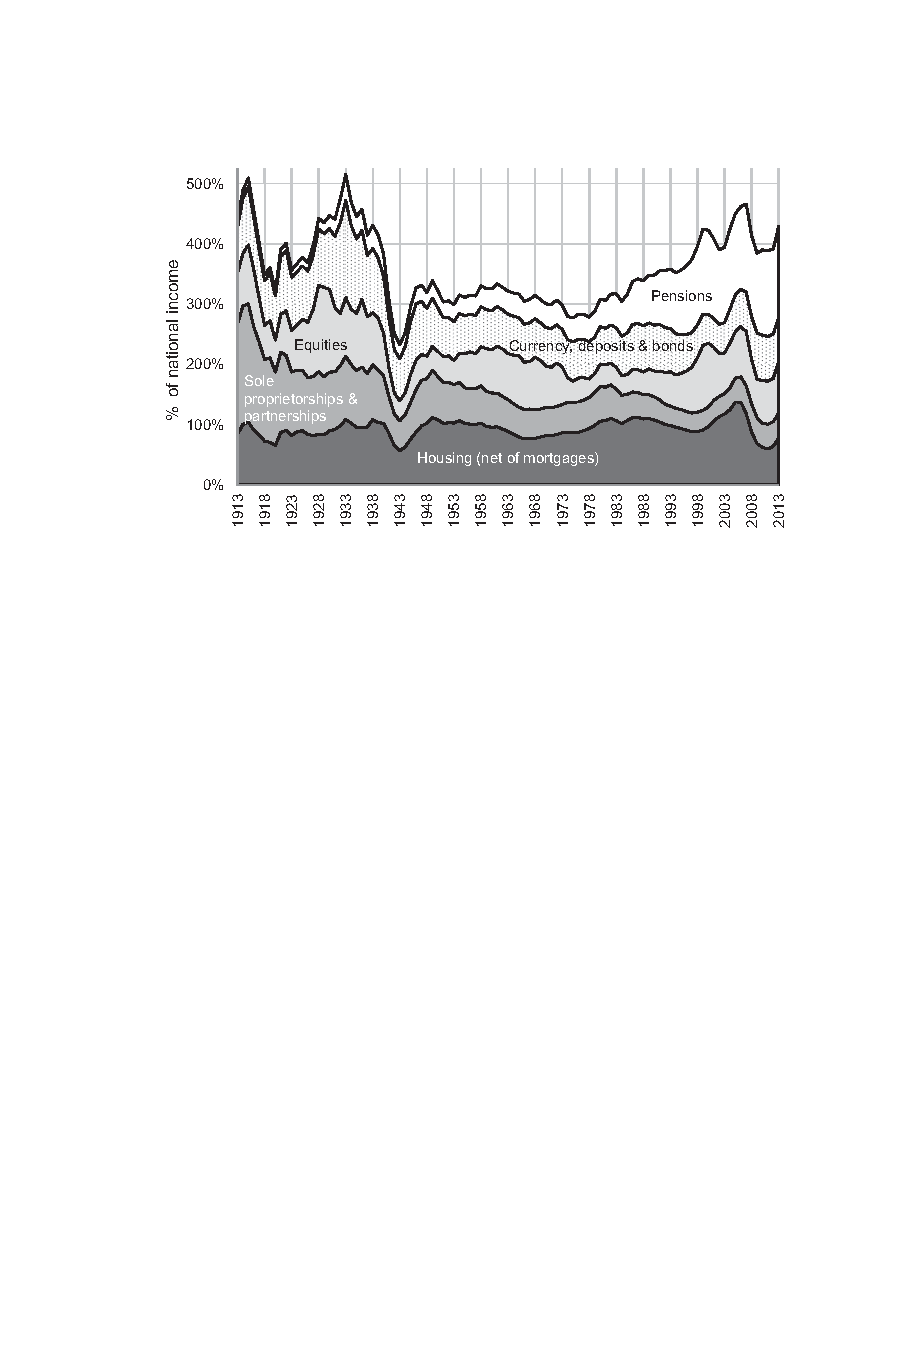
\includegraphics[width=1\linewidth]{figures/fig2-nolegend2} 

}

\caption{\textsc{Aggregate US Household Wealth,
1913--2013}.}\label{fig:saez-zucman-fig2}
\end{figure}

Figure \ref{fig:saez-zucman-fig9a} shows the saving rate by wealth
class, which echoes the evidence on saving rate by income shown
previously in \protect\hyperlink{two-period}{Lecture 3}.



\begin{figure}

{\centering 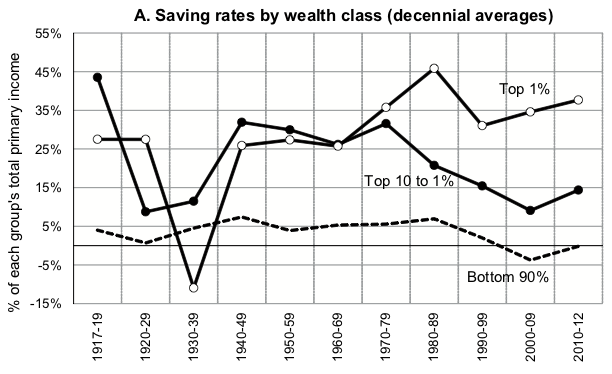
\includegraphics[width=1\linewidth]{figures/fig9a} 

}

\caption{\textsc{Saving Rate by Wealth Class}.}\label{fig:saez-zucman-fig9a}
\end{figure}

Figure \ref{fig:saez-zucman-fig6a} shows the top 10\% wealth share. As
you can see, nearly 75\% of household wealth is held by the top 10\%
wealth owners. This is more concentrated than labor income (the top 10\%
in the United States gets about 50\% of pre-tax income, and much less
after-tax), and therefore does not appear to be solely accounted for by
saving for retirement.



\begin{figure}

{\centering 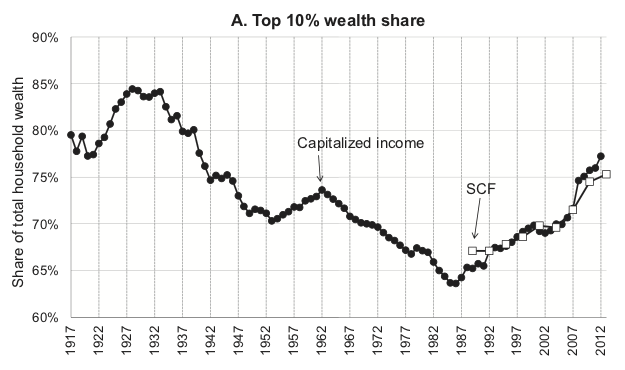
\includegraphics[width=1\linewidth]{figures/fig6a} 

}

\caption{\textsc{Top 10 per cent wealth share}.}\label{fig:saez-zucman-fig6a}
\end{figure}

Figure \ref{fig:saez-zucman-fig6b} shows the top 1\% wealth share, and
the top 1-10\% wealth share. As you can see, the top 1\% now owns nearly
40\% of the wealth in the United States, while it only accounts for
about 20-25\% of pre-tax income. Again, it does not seem like saving for
retirement is the whole story.




\begin{figure}

{\centering 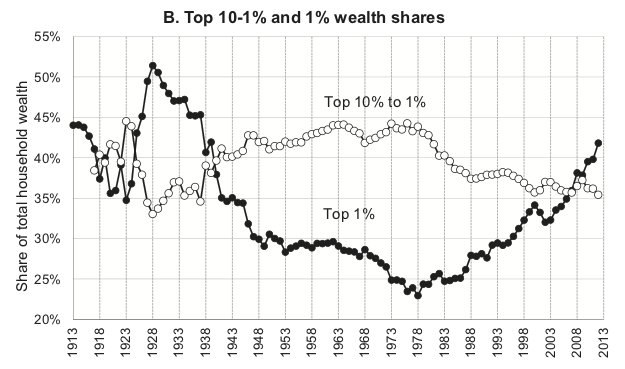
\includegraphics[width=1\linewidth]{figures/fig6b} 

}

\caption{\textsc{Top 1-10 per cent and Top 1 per cent
wealth share}.}\label{fig:saez-zucman-fig6b}
\end{figure}

\subsection{Saving of the rich}\label{saving-of-the-rich}

Understanding the sources of the capital stock amounts to a first order
to undertand the saving of people with very high net worth. What leads
high income and high net worth people to save so much? A number of
explanations have been proposed:

\begin{enumerate}
\def\labelenumi{\arabic{enumi}.}
\item
  \textbf{Leaving bequests.} One reason why people might want to save
  over and above what they need to provide for retirement, is to leave
  bequests. However, it has been shown that even high income workers
  without children save a lot, more than warranted by their retirement
  needs.
\item
  \textbf{Prestige.} Wealth brings prestige. Adam Smith has a great
  passage in The \emph{Theory of Moral Sentiments}, published in 1759:
\end{enumerate}

\begin{quote}
To what purpose is all the toil and bustle of the world?\ldots{} lt is
our vanity which urges us on\ldots{} It is not wealth that men desire,
but the consideration and good opinion that wait upon riches.
\end{quote}

\begin{enumerate}
\def\labelenumi{\arabic{enumi}.}
\setcounter{enumi}{2}
\tightlist
\item
  \textbf{Concern for relative wealth.} Related to this explanation is a
  concern not for the absolute level of wealth per se, but for a
  relative standing compared to others in society. This is for example
  echoed in an academic article, published in 1992:\footnote{Harold L.
    Cole, George J. Mailath, and Andrew Postlewaite, ``Social Norms,
    Savings Behavior, and Growth,'' Journal of Political Economy 100,
    no. 6 (December 1, 1992): 1092--1125,
    \url{https://doi.org/10.1086/261855}.}
\end{enumerate}

\begin{quote}
But think for a moment about an already very rich agent such as Donald
Trump. Why does he continue to work long days, endure substantial
amounts of stress, and take enormous risks? Surely it cannot be that he
is savoring the prospect of going to the grocery store with a looser
budget constraint next year. He seems to have more money than he could
spend in several lifetimes. Even if we are wrong about Trump's net
worth, there clearly seem to be wealthy individuals that continue to
work very hard and take large risks to increase their net worth. It is
hard to reconcile such behavior with the underlying decision making in
traditional growth models. We propose that people like Trump continue to
care about increasing their net worth because their utility depends not
only on the absolute level of their wealth but also on their wealth
relative to that of other very rich people.
\end{quote}

\begin{enumerate}
\def\labelenumi{\arabic{enumi}.}
\setcounter{enumi}{3}
\tightlist
\item
  \textbf{Religious beliefs and work ethic.} Max Weber has famously
  proposed the protestant work ethic in
  \href{https://en.wikipedia.org/wiki/The_Protestant_Ethic_and_the_Spirit_of_Capitalism}{The
  Protestant Ethic and the Spirit of Capitalism} as one explanation for
  the emergence of capitalism, and the importance of hard work and
  saving. John Maynard Keynes, in the
  \href{https://socialsciences.mcmaster.ca/econ/ugcm/3ll3/keynes/pdf\%26filename\%3Dpeace3.pdf}{Economic
  Consequences of the Peace} published in 1919, was thinking very much
  in these terms:
\end{enumerate}

\begin{quote}
Europe was so organised socially and economically as to secure the
maximum accumulation of capital. While there was some continuous
improvement in the daily conditions of life of the mass of the
population, society was so framed as to throw a great part of the
increased income into the control of the class least likely to consume
it. The new rich of the nineteenth century were not brought up to large
expenditures, and preferred the power which investment gave them to the
pleasures of immediate consumption. In fact, it was precisely the
inequality of the distribution of wealth which made possible those vast
accumulations of fixed wealth and of capital improvements which
distinguished that age from all others. Herein lay, in fact, the main
justification of the capitalist system. If the rich had spent their new
wealth on their own enjoyments, the world would long ago have found such
a régime intolerable. But like bees they saved and accumulated, not less
to the advantage of the whole community because they themselves held
narrower ends in prospect.
\end{quote}

\begin{quote}
The immense accumulations of fixed capital which, to the great benefit
of mankind, were built up during the half century before the war, could
never have come about in a society where wealth was divided equitably.
The railways of the world, which that age built as a monument to
posterity, were, not less than the pyramids of Egypt, the work of labour
which was not free to consume in immediate enjoyment the full equivalent
of its efforts.
\end{quote}

\begin{quote}
Thus this remarkable system depended for its growth on a double bluff or
deception. On the one hand the labouring classes accepted from ignorance
or powerlessness, or were compelled, persuaded, or cajoled by custom,
convention, authority, and the well-established order of society into
accepting, a situation in which they could call their own very little of
the cake that they and nature and the capitalists were co-operating to
produce. And on the other hand the capitalist classes were allowed to
call the best part of the cake theirs and were theoretically free to
consume it, on the tacit underlying condition that they consumed very
little of it in practice. The duty of 'saving' became nine-tenths of
virtue and the growth of the cake the object of true religion. There
grew round the non-consumption of the cake all those instincts of
puritanism which in other ages has withdrawn itself from the world and
has neglected the arts of production as well as those of enjoyment. And
so the cake increased; but to what end was not clearly contemplated.
Individuals would be exhorted not so much to abstain as to defer, and to
cultivate the pleasures of security and anticipation. Saving was for old
age or for your children; but this was only in theory -- the virtue of
the cake was that it was never to be consumed, neither by you nor by
your children after you.
\end{quote}

\begin{enumerate}
\def\labelenumi{\arabic{enumi}.}
\setcounter{enumi}{4}
\tightlist
\item
  \textbf{A final hypothesis.} An even more mundane explanation (which
  does not make it wrong!) has been proposed by Lee Iacocca, former CEO
  from Chrysler. According to him, the rich simply do not know what to
  do with their money:
\end{enumerate}

\begin{quote}
Once you reach a certain level in a material way, what more can you do?
You can't eat more than three meals a day; you'll kill yourself. You
can't wear two suits one over the other. You might now have three cars
in your garage-but six! Oh, you can indulge yourself, but only to a
point.
\end{quote}

Most economists are however general skeptical of this type of
explanations. What they find puzzling is that high net worth individuals
keep working even when they have achieved a sufficient amount of
wealth.\footnote{I personally am less sure, as culture and norms
  certainly play a bigger role than many economists imagine - for
  example, as explained above, the protestant work ethic, might be one
  answer.}

All this discussion may seem like armchair theorizing. At the same time,
these are probably the most important questions facing macroeconomics.
They actually determine the stance that should be taken on optimal
capital accumulation, the optimal level of public debt, etc. We shall
come back to these issues repeatedly in the following lectures.

\hypertarget{technology}{\chapter{Technological
Change}\label{technology}}

In this lecture, we start by reviewing
\protect\hyperlink{long-run-growth}{some facts on long-run economic
growth}. We then review \protect\hyperlink{endogenous-growth-model}{an
endogenous growth model} which tries to account for long-run economic
growth.

\hypertarget{long-run-growth}{\section{Long-run Economic
Growth}\label{long-run-growth}}

In this section, we remind ourselves some basic facts on technological
growth since the 1200s. We in particular use Angus Maddison's long run
data series on GDP per capita in major advanced economies, to show that
growth as we know it is a rather recent phenomenon, one that starts at
the beginning of the nineteenth century.

\subsection{The Facts of Growth}\label{the-facts-of-growth}

The Figures below show GDP per capita in France, Germany, Italy, the
United Kingdom, and the United States, starting respectively in 1200,
1700, 1800, and 1900. These are presented on a semi-logarithmic scale
(that is, the y-axis is in log), also sometimes called a ratio scale. Do
not worry too much about the unit in which GDP per capita is expressed
in this Maddison data: the unit is called the
\href{https://en.wikipedia.org/wiki/Geary\%E2\%80\%93Khamis_dollar}{Geary--Khamis
dollar}, but we shall come back to it when we discuss the issue of real
exchange rates and purchasing power parity comparisons. The reason for
using such a semi-logarithmic scale is that growth is roughly
exponential, so it is approximately linear on a semi-logarithmic scale.



\begin{figure}

{\centering 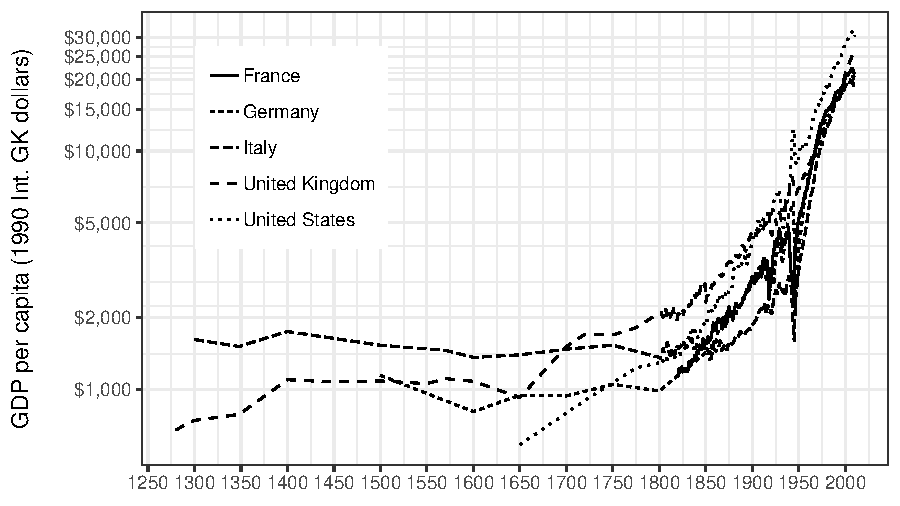
\includegraphics[width=1\linewidth]{ucla-102-fall2018_files/figure-latex/gdp-1200-1} 

}

\caption{\textsc{1200-2010 GDP per capita (Maddison Data)}.}\label{fig:gdp-1200}
\end{figure}



\begin{figure}

{\centering 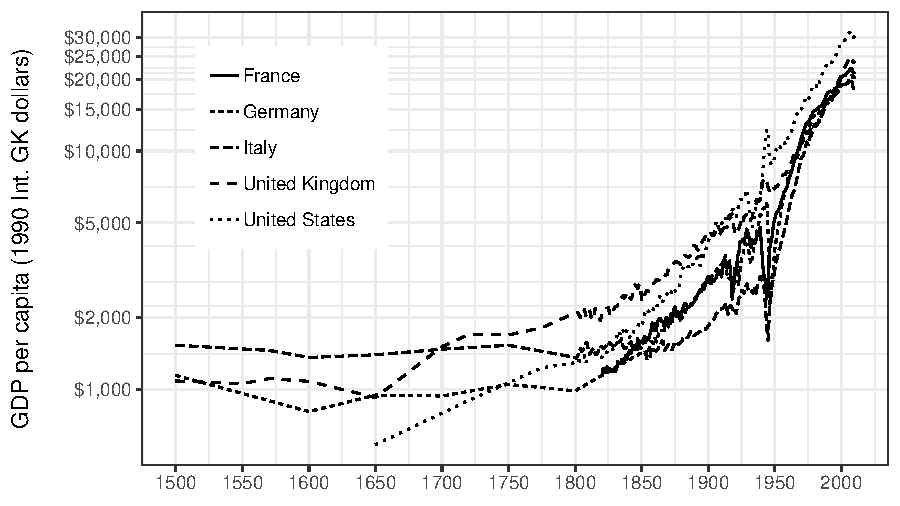
\includegraphics[width=1\linewidth]{ucla-102-fall2018_files/figure-latex/gdp-1700-1} 

}

\caption{\textsc{1700-2010 GDP per capita (Maddison Data)}.}\label{fig:gdp-1700}
\end{figure}



\begin{figure}

{\centering 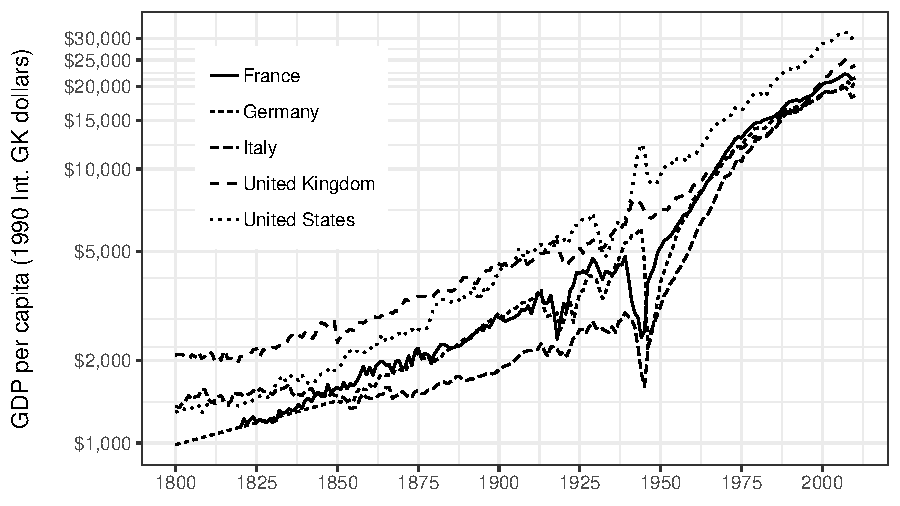
\includegraphics[width=1\linewidth]{ucla-102-fall2018_files/figure-latex/gdp-1800-1} 

}

\caption{\textsc{1800-2010 GDP per capita (Maddison Data)}.}\label{fig:gdp-1800}
\end{figure}



\begin{figure}

{\centering 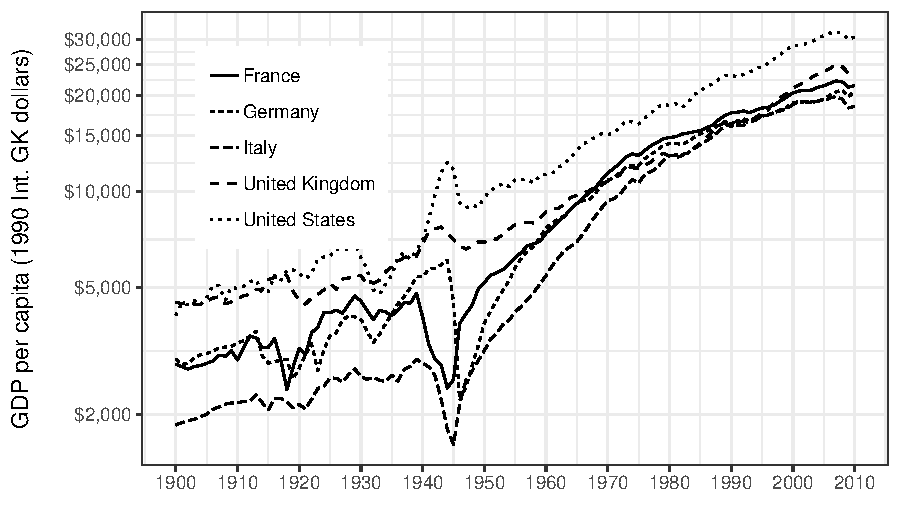
\includegraphics[width=1\linewidth]{ucla-102-fall2018_files/figure-latex/gdp-1900-1} 

}

\caption{\textsc{1900-2010 GDP per capita (Maddison Data)}.}\label{fig:gdp-1900}
\end{figure}

\subsection{The Mathematics of Growth}\label{the-mathematics-of-growth}

The mathematical orders of magnitude with exponential growth are
sometimes hard to grasp intuitively. This section provides you with some
maths to help get an intuitive feel for exponential growth. Let's
consider an economic quantity \(y_t\), growing at a constant rate \(g\).
For our purposes in this lecture, \(y_t\) is GDP per capita, but it
could also veru well be a price level, consumption, or some other
economic quantity. Iterating on the difference equation allows to get
\(y_t\) as a function of the initial value: \[
\begin{aligned}
y_t = (1+g)y_{t-1} \quad \Rightarrow \quad y_t = (1+g)^t y_0.
\end{aligned}
\] How fast of a growth is that? The number of years \(T\) it takes for
GDP per capita to be multiplied by a factor \(F\) (where \(F=2\), if we
are looking for GDP to double) is given by : \[
\begin{aligned}
&y_t = F y_0 \quad \Rightarrow \quad (1+g)^t y_0 = F y_0 \quad \Rightarrow \quad (1+g)^T = F \\
& \quad \Rightarrow \quad \ln (1+g)^T = \ln F \quad \Rightarrow \quad T \ln (1+g) = \ln F \\
& \quad \Rightarrow \quad T=\frac{\ln F}{\ln(1+g)}.
\end{aligned}
\] For small rates of growth, we know that a Taylor expansion of the
\(\ln\) gives \(\ln(1+g)=g\), so that this formula can be approximated
by: \[T = \frac{\ln F}{g}.\]

\textbf{Rule of 70.} This formula gives the ``rule of 70'' for small
growth rates. The ``rule of 70'' states that a quantity which grows at a
rate \(g\) in percentage terms, takes approximately \(70/g\) years to
double. This comes from the fact that \(100*ln(2) \approx\) 69.3147181.
For example, if GDP per capita is growing at 2\% per year, then it takes
approximately 35 years for it to double: approximately one generation
only. If it is growing at 1\% per year, it takes approximately 70 years
for it to double, so two generations. Whether you grow to be twice as
rich as your parents, or twice as rich as your grandparents on average
makes a big difference.

\textbf{Rule of 230.} The same formula also gives the ``rule of 230''
for small growth rates. The ``rule of 230'' states that a quantity which
grows at a rate \(g\) in percentage terms, takes approximately \(230/g\)
years to be multiplied by \(10\). This is because:
\(100*ln(10) \approx\) 230.2585093. Thus, with a 2\% growth rate, GDP
per capita is multiplied by \(10\) over (as an exercise, you may create
your own rules\ldots{})

\subsection{Questions}\label{questions}

The \protect\hyperlink{long-run-growth}{previous section} has shown that
economic growth has been 2\% on average in advanced economics, in the
last two centuries. This raises a number of questions.

\textbf{Why is there GDP per capita growth at all?} One major
shortcoming of Bob Solow's Growth model of
\protect\hyperlink{solow}{Lecture 2} and of Peter Diamond's growth model
of \protect\hyperlink{olg}{Lecture 4} is that they fail to account for
long run economic growth - rather ironically. According to these models,
the process of capital accumulation reaches a steady-state at some
point, such that capital per capita, GDP per capita, remain forever
constant. This happens for intuitive reasons: if the labor force is
given, then growth cannot be sustained through capital accumulation
alone. In fact, in the Solow model, even a saving rate equal to 100\%
would lead to very high GDP, but not to constant GDP growth. At one
point, the capital stock would be so large that merely maintaining it
would consume all output. Output would then be equal to gross saving,
and depreciation. This is coming from the fact that at the steady state
of the Solow model, gross saving is given by \(s Y^{*}\) which would
then be equal to \(Y^{*}\) (if \(s=1=100\%\)), which is also equal to
depreciation as: \[s Y^{*}=\delta K^{*}.\]

\textbf{The Cross-section of Countries: Rich versus Poor Countries.} The
power of compounding is such that even a few decades of lower growth
makes a big difference. Given persistent differences in growth rates,
per capita GDP is far from being equalized across countries. Contrary to
the predictions in the Solow growth model, there has hardly been a
strong catch up of poor countries towards the level of rich countries.
On one hand of the spectrum, many countries have very small GDP per
capita levels.




\begin{table}

\caption{\label{tab:low-gdp-per-cap}\textsc{Countries with GDP per capita lower than
\$1.5K.}}
\centering
\begin{tabular}[t]{cc}
\toprule
Country & GDP per capita\\
\midrule
Ethiopia & \$ 1,489\\
Togo & \$ 1,446\\
Sierra Leone & \$ 1,353\\
Guinea-Bissau & \$ 1,257\\
Madagascar & \$ 1,237\\
\addlinespace
Mozambique & \$ 1,211\\
D.R. of the Congo & \$ 1,199\\
Malawi & \$ 971\\
Liberia & \$ 877\\
Niger & \$ 868\\
\addlinespace
Burundi & \$ 840\\
Central African Republic & \$ 599\\
\bottomrule
\end{tabular}
\end{table}




\begin{figure}

{\centering 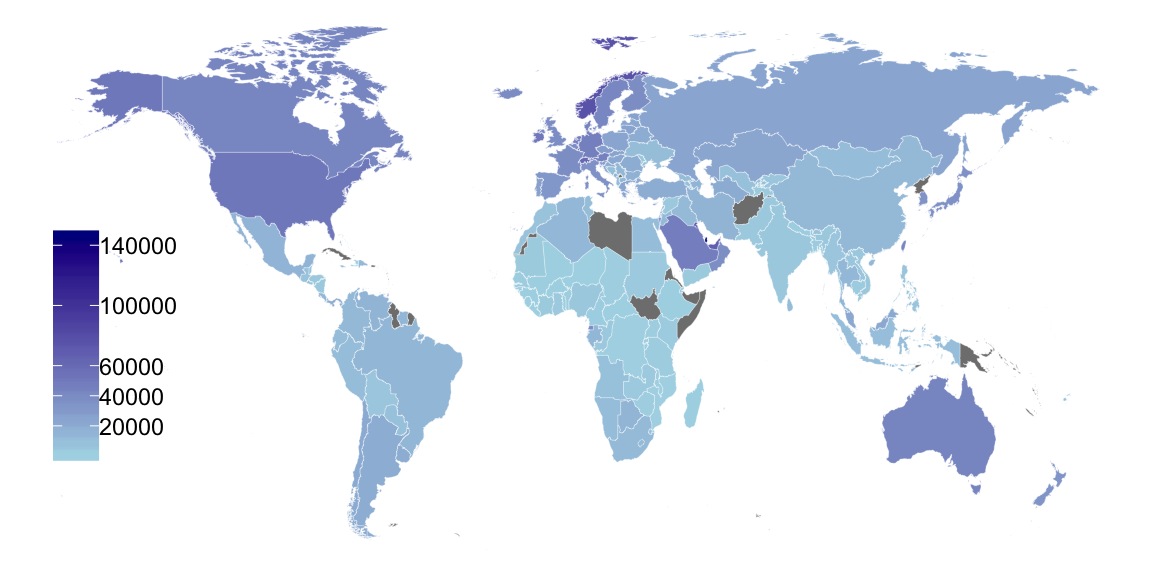
\includegraphics[width=1\linewidth]{ucla-102-fall2018_files/figure-latex/map-gdp-per-capita-1} 

}

\caption{\textsc{2014 GDP per capita, by Country (Penn
World Tables)}.}\label{fig:map-gdp-per-capita}
\end{figure}

On the other, some countries have very high GDP per capita. Table
\ref{tab:high-gdp-per-cap} below shows the countries that have a GDP per
capita higher than \$40K.




\begin{table}

\caption{\label{tab:high-gdp-per-cap}\textsc{Countries with GDP per capita higher than
\$40K.}}
\centering
\begin{tabular}[t]{cc}
\toprule
Country & GDP per capita\\
\midrule
Qatar & \$ 146,037\\
China, Macao SAR & \$ 130,758\\
Norway & \$ 75,920\\
United Arab Emirates & \$ 68,021\\
Kuwait & \$ 67,432\\
\addlinespace
Brunei Darussalam & \$ 66,968\\
Singapore & \$ 66,050\\
Luxembourg & \$ 65,842\\
Switzerland & \$ 61,570\\
United States & \$ 51,623\\
\addlinespace
Ireland & \$ 51,224\\
Netherlands & \$ 47,392\\
Saudi Arabia & \$ 46,772\\
Germany & \$ 46,190\\
China, Hong Kong SAR & \$ 45,399\\
\addlinespace
Austria & \$ 45,158\\
Denmark & \$ 43,733\\
Australia & \$ 43,590\\
Canada & \$ 42,794\\
Sweden & \$ 42,117\\
Taiwan & \$ 41,514\\
\bottomrule
\end{tabular}
\end{table}

Why are poor countries so poor, and largely failing to catch up, and why
advanced economies are growing at an average of 2\% per year since the
beginning of the nineteenth century, are perhaps the potentially most
impactful questions for economics, but also those for which economists
perhaps know the least. This lecture presents an attempt at endogenizing
GDP per capita growth, based on the a very simplified version of
\href{https://en.wikipedia.org/wiki/Paul_Romer}{Paul Romer}'s endogenous
growth model. This may allow us to shed light on some of these issues.

\hypertarget{endogenous-growth-model}{\section{Endogenous Growth
Model}\label{endogenous-growth-model}}

Paul Romer was awarded the Nobel Prize in Economic Sciences this year.
\href{https://www.economist.com/finance-and-economics/2018/10/13/paul-romer-and-william-nordhaus-win-the-economics-nobel?fsrc=scn/fb/te/bl/ed/paulromerandwilliamnordhauswintheeconomicsnobelfreeexchange}{The
Economist} is a good coverage of his work. In this section, we present a
very simplified version of his much more subtle ideas.

\subsection{Objects VS Ideas}\label{objects-vs-ideas}

A crucial distinction for understanding endogenous growth theory, is
that of objects versus ideas.

\textbf{Objects.} Objects like houses, food, or cell phones are
\textbf{rivalrous}. That is, one person's use of one of these particular
objects prevents its use by someone else. Most goods are rivalrous, and
this is what leads to scarcity, the central topic of economics.

\textbf{Ideas and recipes.} In contrast, ideas are \textbf{nonrival}. My
use of an idea does not prevent someone else's use of that idea. For
example, after it has been shot, a movie can be shown in any theatre in
the world, and for a cost equal to zero on the internet (apart for the
cost of electricity, and of storing the movie on servers). Similarly, a
recipe for a pharmaceutical drug takes years to develop. However, once
the drug has been invented, the cost of producing this drug is typically
very small, much smaller than the associated initial fixed cost.
Finally, Antonín Dvořák's 9th Symphony ``From the New World'' can be
performed by any orchestra in the world,
\href{https://www.youtube.com/watch?v=vHqtJH2f1Yk}{Gustavo Dudamel's} or
\href{https://www.youtube.com/watch?v=0hmjGbh9qdg\&start_radio=1\&list=RD0hmjGbh9qdg\&t=193}{Herbert
Von Karajan's}, once Antonín Dvořák has composed it.

According to Paul Romer, ideas and recipes have the potential to be a
source of indefinite economic growth:

\begin{quote}
Every generation has perceived the limits to growth that finite
resources and undesirable side effects would pose if no new recipes or
ideas were discovered. And every generation has underestimated the
potential for finding new recipes and ideas. We consistently fail to
grasp how many ideas remain to be discovered.
\end{quote}

As Chad Jones puts it describing Paul Romer's contributions in a
\href{https://voxeu.org/article/new-ideas-about-new-ideas-paul-romer-nobel-laureate}{Vox
Eu article}:

\begin{quote}
Once you've got increasing returns, growth follows naturally. Output per
person then depends on the total stock of knowledge; the stock doesn't
need to be divided up among all the people in the economy. Contrast this
with capital in a Solow model. If you add one computer, you make one
worker more productive. If you add a new idea -- think of the computer
code for the first spreadsheet or word processor or even the internet
itself -- you can make any number of workers more productive. With
non-rivalry, growth in income per person is tied to growth in the total
stock of ideas -- an aggregate -- not to growth in ideas per person.
\end{quote}

However, ideas implies increasing returns and therefore, potentially
inefficient market outcomes.

\subsection{Increasing Returns}\label{increasing-returns}

Because of increasing returns, a competitive market economy may not lead
to an efficient level of development of ideas. The issue with pure
competition is that if a movie director was forced to charge a price
equal to the marginal cost of showing a movie, then he would have to
charge a zero price for this movie, as it would then be available for
everyone to watch on Youtube. Similarly, once a drug against AIDS (for
example) has been invented, one would ideally like to give this drug to
the largest possible number of people. Indeed, the marginal cost of
producing a new drug is much lower than the cost at which it is
commercialized. However, this would decrease the incentives to innovate
in the first place.

\textbf{Patents.} One way that this market failure has historically been
addressed, is by granting patents (property rights) on newly invented
ideas. (in biology, scientists are sometimes granted 12 years of
exclusivity; in chemistry, they may be granted 5 years) Similarly,
intellectual property rights, as well as laws against piracy, have the
same purpose: they seek to encourage innovation by preventing 0 marginal
cost pricing. Note however that patents should not be too strong either,
or they discourage the use of new ideas, potentially at a suboptimal
level. In fact, historically, especially in periods of high innovation
and economic growth, intellectual property rights were relatively weak.
When the US was a rising economic power, it was also a notorious pirate
of intellectual property, very much like what China is being accused of
today.

\textbf{Government funded research.} One alternative way through which
R\&D can be incentivized, while allowing for large dissemination, is to
have the allow for government funded research. For example, the
Department of Defense's ARPANET was a precursor of today's World Wide
Web.

\textbf{Prizes.} Another way for the government to incentivize
fundamental research is to give out prizes, which are a rather
inexpensive way to motivate researchers hoping for recognition. The
Economics Nobel Prize is one such example. In general, the motivations
of researchers are complex, and probably not purely driven by profit
seeking. For example, a very large community of developers contributes
to open-source software, which is hard to rationalize from an orthodox
(individualist) economic standpoint.

\subsection{Model}\label{model}

In Paul Romer's endogenous growth model, there are two types of workers:
research workers, whose number is \(L_{at}\), and production workers,
whose number is \(L_{yt}\). We denote the share of research workers in
total labor by \(l\), so that: \[L_{at} = l L\] The number of production
workers is simply the complement of that, so that: \[L_{yt} = (1-l)L.\]
As an example, if \(l=0.10\), then 10\% of the labor force works in the
R\&D sector. For simplicity, we neglect the role of capital and capital
accumulation, an issue that you will take up during sections. Therefore,
production is simply given by: \[Y_{t} =A_{t} L_{yt}\]

Finally, productivity is assumed to grow at a rate that is function of
the productivity of the research sector \(z\), overall productivity
\(A_t\), and the number of researchers in the research sector
\(L_{at}\): \[\Delta A_{t+1} =z A_{t} L_{at}.\]

\subsection{Solution}\label{solution-2}

In order to solve this model, we may simply iterate on the production
function for new ideas, as a function of the initial value for
productivity \(A_0\) (just as there was an initial value for capital
\(K_0\) in the Solow growth model), and using that the number of
research workers is \(L_{at} = l L\): \[
\begin{aligned}
& \Delta A_{t+1} = A_{t+1}-A_t =z A_{t} L_{at}\\
& \quad \Rightarrow \quad  A_{t+1} = (1+z L_{at})A_{t} \\
& \quad \Rightarrow \quad  A_{t+1}=\left(1+zlL\right)A_{t}\\
& \quad \Rightarrow \quad  A_{t}=\left(1+zlL\right)^{t}A_{0}.
\end{aligned}
\] Replacing then \(L_{yt}\) in the production function with
\(L_{yt} = (1-l)L\), as well as this endogenous level of productivity,
we get: \[
\begin{aligned}
Y_{t}&  =A_{t} L_{yt}\\
&= \left(1+zlL\right)^{t}A_{0}L_{yt}\\
&= \left(1+zlL\right)^{t}A_{0}(1-l)L\\
Y_{t}&= A_{0}(1-l)L \left(1+zlL\right)^{t}
\end{aligned}
\]

\textbf{Change in \(l\).} A change on the research share of workers has
too opposing effect. On the one hand, there are less production workers
available for production Thus, there is a fall in \(L_{yt}\), which
tends to reduce \(Y_t\). On the other, overall growth, which is here
given by \(g = zlL\), is then permanently higher.

\subsection{Shortcomings}\label{shortcomings}

In Paul Romer's model, all economic growth comes from R\&D. Despite its
successes, this model however leaves a number of questions unanswered.
For example, it is unclear why poor countries are not able to benefit
from ``ideas'' which are available in rich countries. Ideas being a
public good, they are potentially available for anyone to use. Then,
productivity \(A_t\) should be quite similar in rich and poor countries.
Moreover, the endogenous growth model does not really explain why
economic growth took off where and when it took off (in the UK, at the
beginning of the nineteenth century), a question we started out with.

If you want to know more, this
\href{https://www.economist.com/finance-and-economics/2018/04/12/economists-understand-little-about-the-causes-of-growth}{Economist
article} gives a number of limitations on the theory of economic growth.
In particular, economic historians are still debating the origins of the
Industrial Revolution. Important factors that the endogenous growth
model neglects are the relative importance of \textbf{secure property
rights}, the extent to which cultures tolerate \textbf{personal
ambition}, and other cultural or political factors, all of which
certainly matter for economic growth. You may refer to the next section,
if you wish to read more about economic growth.

\section*{Readings - To go further}\label{readings---to-go-further-2}
\addcontentsline{toc}{section}{Readings - To go further}

\href{https://doi.org/10.1257/jep.27.1.3}{Michele Boldrin and David K.
Levine, ``The Case against Patents,'' Journal of Economic Perspectives
27, no. 1 (February 2013): 3--22.}

\href{https://voxeu.org/article/new-ideas-about-new-ideas-paul-romer-nobel-laureate}{Chad
Jones, New ideas about new ideas: Paul Romer, Nobel laureate, \emph{Vox
Eu}, October 12, 2018.}

\href{https://search.proquest.com/docview/2123033147/1417E92D94B43EFPQ/3?accountid=14512}{Paul
Krugman, Notes on Global Convergence (Wonkish and Off-Point), \emph{New
York Times}, October 20, 2018.}

(Gated)
\href{https://www.economist.com/news/leaders/21660522-ideas-fuel-economy-todays-patent-systems-are-rotten-way-rewarding-them-time-fix}{Time
to fix patents, \emph{The Economist}, August 8 2015.}

(Gated)
\href{https://www.economist.com/international/2015/08/08/a-question-of-utility}{A
question of utility, \emph{The Economist}, August 8, 2015.}

(Gated)
\href{https://www.economist.com/finance-and-economics/2018/04/12/economists-understand-little-about-the-causes-of-growth}{Economists
understand little about the causes of growth, \emph{The Economist},
April 12, 2018.}

(Gated)
\href{https://www.economist.com/finance-and-economics/2018/10/13/paul-romer-and-william-nordhaus-win-the-economics-nobel?fsrc=scn/fb/te/bl/ed/paulromerandwilliamnordhauswintheeconomicsnobelfreeexchange}{Paul
Romer and William Nordhaus win the economics Nobel, \emph{The
Economist}, Oct 13, 2018.}

\hypertarget{labor-market}{\chapter{The Labor Market and
Unemployment}\label{labor-market}}

This lecture goes over three different models of the labor market, each
of which has a different explanation for the phenomenon of unemployment:
\protect\hyperlink{neoclassical}{the Neoclassical model},
\protect\hyperlink{keynesian}{the Keynesian model},
\protect\hyperlink{bathtub}{the Bathtub model}. In this lecture, we
examine each of them in turn.

\hypertarget{neoclassical}{\section{The Neoclassical
Model}\label{neoclassical}}

\subsection{Assumptions}\label{assumptions-3}

Neoclassical economic theory is fundamentally based on the laws of
supply and demand. In this theory, labor is treated as another good,
which enters negatively in the utility function of workers because
people would rather not work (therefore, labor is a ``bad'' rather than
a ``good''). Labor is also a useful input into production, which allows
firms to sell consumption goods to workers. In the neoclassical theory,
the real wage is determined at the intersection of supply and demand.

\textbf{Labor Demand.} Firms hire labor at price \(w\), and sell the
consumption good a price \(p\). Assume that the production function is
decreasing returns to scale with respect to labor (think for example,
that the quantity of capital is fixed): \[y = f(l).\] Then, firms
maximize their profits, and therefore solve:
\[\max_l \quad pf(l) - wl.\]

\textbf{Labor Supply.} Neoclassical theory of labor supply starts from a
static problem of a consumer-worker choosing how much to work, and how
much to consume. For example, assume that utility is strictly increasing
in consumption, and strictly decreasing in the amount of labor supplied:
\[U(c, l)=u(c)-v(l),\] so that the consumer-worker likes to consume, but
does not like working. If the price of consumption is \(p\), and
assuming a static problem, the budget constraint of a worker/consumer is
given by: \[pc = wl.\] You may think of \(w\) as the hourly wage, for
example \$15/hour. Then \(l\) would be expressed in terms of the number
of hours.

\emph{Warning}. Labor Supply and Labor Demand are sometimes being mixed
up. In the language of microeconomics, workers supply labor, and firms
demand labor. What workers do demand is jobs, or job vacancies, which
are supplied by firms.

\subsection{Solution}\label{solution-3}

\textbf{Labor Demand.} The problem of labor demand shown above leads to
the following first-order condition:
\[pf'(l)-w = 0 \quad \Rightarrow \quad f'(l)=\frac{w}{p}.\] This
equation has a straightforward interpretation: at the optimum, the
marginal product of labor - that is, how much is gained from using one
more unit of labor in production \(f'(l)\) - needs to be equal to how
much that additional unit of labor costs to the firm, the real wage
\(w/p\). J.M. Keynes calls it the first fundamental postulate of
classical economics in Chapter 2 of the
\href{http://cas2.umkc.edu/economics/people/facultypages/kregel/courses/econ645/winter2011/generaltheory.pdf}{General
Theory}.

\textbf{Labor Supply.} On the other hand, the problem of the consumer
consists in maximizing utility under his budget constraint: \[
\begin{aligned}
\max_{c,l}& \quad u(c)-v(l),\\
&\text{s.t.}\quad p \cdot c = w \cdot l.
\end{aligned}
\]

Again, similarly to the two-period optimization problem of
\protect\hyperlink{two-period}{Lecture 3}, you may solve this
optimization in four different ways:

\begin{enumerate}
\def\labelenumi{\arabic{enumi}.}
\item
  You may compute the ratio of marginal utilities (the marginal rate of
  substitution between consumption and labor) and state that it is equal
  to minus the real wage (because labor slackens the intertemporal
  budget constraint, and it appears on the right hand-side of the equal
  sign):
  \[\frac{\partial U / \partial l}{\partial U / \partial c} = -\frac{w}{p} \quad\Rightarrow\quad \boxed{\frac{v'(l)}{u'(c)}=\frac{w}{p}}\]
\item
  You may apply the following intuitive economic argument. The marginal
  disutility from supplying one more unit of labor is \(v'(l)\), for a
  worker already supplying \(l\) units of them. The marginal utility
  which is gained from doing so is given by the number of additional
  units of consumption one gets out of it, given by the real wage
  \(w/p\), and by how much I value each one of these additional
  utilities of consumption is valued, given by marginal utility
  \(u'(c)\). The total gain in utility from consumption is the unit
  value \(u'(c)\) times the number of units \(w/p\), which gives the
  result:
  \[v'(l)=\frac{w}{p}u'(c)\quad \Rightarrow \quad \boxed{\frac{v'(l)}{u'(c)}=\frac{w}{p}.}\]
  J.M. Keynes, who did not write one equation in his General Theory,
  calls this the second postulate of the classical economics, in Chapter
  2: ``The utility of the wage when a given volume of labour is employed
  is equal to the marginal disutility of that amount of employment.''
\item
  You may substitute out \(l\) from the budget constraint, and optimize
  over the choice of consumption:
  \[\max_c \quad u(c)-v\left(\frac{p}{w} c\right).\] This implies:
  \[u'(c)-\frac{p}{w}v'(l)=0 \quad \Rightarrow \quad \frac{v'(l)}{u'(c)}=\frac{w}{p}.\]
\item
  You may substitute out \(c\) from the budget constraint, and optimize
  over the choice of labor:
  \[\max_l \quad u\left(\frac{w}{p}l\right)-v(l).\] This implies:
  \[\frac{w}{l}u'(c)-v'(l)=0 \quad \Rightarrow \quad \boxed{\frac{v'(l)}{u'(c)}=\frac{w}{p}}.\]
\end{enumerate}

\subsection{A Simple Example}\label{a-simple-example}

\textbf{Assumptions.} Assume a Cobb-Douglas production function for
\(f(l)\), such that: \[f(l)=A l^{1-\alpha}.\] In the background, you can
really think that the capital stock is exogenous and taken to be equal
to \(K=1\), which would lead to this production function exactly.

Let us also assume linear utility for consumption (that is, people enjoy
increasing utility equally, regardless of whether it is coming from the
first dollar or the last one - this assumption is not realistic and is
really made for simplicity), as well as a power function of disutility
for work: \[u(c)=c, \quad v(l)=B\frac{l^{1+\epsilon}}{1+\epsilon}\] so
that: \[U(c, l)=c-B\frac{l^{1+\epsilon}}{1+\epsilon}.\]

\textbf{Results.} Using the above functional forms for \(u(.)\) and
\(v(.)\) allows to write:
\[v'(l)=Bl^{\epsilon}, \quad u'(c)=1, \quad \Rightarrow \quad Bl^{\epsilon} = \frac{w}{p}.\]
Labor supply \(L^{s}(.)\) as a function of the real wage \(w/p\) is thus
given by:
\[l =\frac{1}{B^{1/\epsilon}} \left(\frac{w}{p}\right)^{1/\epsilon} \equiv L^s\left(\frac{w}{p}\right).\]
Moreover, using the above functional form for \(f(.)\) allows to write:
\[f'(l) =A(1-\alpha)l^{-\alpha} \quad \Rightarrow \quad A(1-\alpha)l^{-\alpha}=\frac{w}{p}.\]
Therefore, labor demand \(L^d(.)\) is given as a function of the real
wage \(w/p\) by:
\[l=A^{1/\alpha}(1-\alpha)^{1/\alpha}\left(\frac{w}{p}\right)^{-1/\alpha}\equiv L^d\left(\frac{w}{p}\right).\]
To sum up, the neoclassical labor makret is composed of the following
labor supply and labor demand equations: \[
\begin{aligned}
L^d\left(\frac{w}{p}\right) &= A^{1/\alpha}(1-\alpha)^{1/\alpha}\left(\frac{w}{p}\right)^{-1/\alpha},\\
L^s\left(\frac{w}{p}\right) &= \frac{1}{B^{1/\epsilon}} \left(\frac{w}{p}\right)^{1/\epsilon}.
\end{aligned}
\] Market clearing implies that labor supply equals labor demand: \[
\begin{aligned}
&L^d\left(\frac{w}{p}\right) = L^s\left(\frac{w}{p}\right) \\
&\quad \Rightarrow \quad A^{1/\alpha}(1-\alpha)^{1/\alpha}\left(\frac{w}{p}\right)^{-1/\alpha} = \frac{1}{B^{1/\epsilon}} \left(\frac{w}{p}\right)^{1/\epsilon} \\
&\quad \Rightarrow \quad \left(\frac{w}{p}\right)^{\frac{1}{\alpha} +\frac{1}{\epsilon}}= (1-\alpha)^{1/\alpha}A^{1/\alpha} B^{1/\epsilon}\\
& \quad \Rightarrow \quad \frac{w}{p} = (1-\alpha)^{\frac{\epsilon}{\alpha+\epsilon}}A^{\frac{\epsilon}{\alpha+\epsilon}} B^{\frac{\alpha}{\alpha+\epsilon}}.
\end{aligned}
\]

We may use either labor supply or labor demand in order to express the
equilibrium quantity of labor \(l\). For example, let us use labor
demand (as an exercise, you may check that using labor supply instead
leads to the same expression): \[
\begin{aligned}
l&=\frac{1}{B^{1/\epsilon}} \left(\frac{w}{p}\right)^{1/\epsilon}\\
&=\frac{1}{B^{1/\epsilon}} (1-\alpha)^{\frac{1}{\alpha+\epsilon}}A^{\frac{1}{\alpha+\epsilon}} B^{\frac{\alpha}{\epsilon(\alpha+\epsilon)}}\\
&= (1-\alpha)^{\frac{1}{\alpha+\epsilon}}A^{\frac{1}{\alpha+\epsilon}} B^{\frac{\alpha}{\epsilon(\alpha+\epsilon)}-\frac{1}{\epsilon}}\\
l&= (1-\alpha)^{\frac{1}{\alpha+\epsilon}}A^{\frac{1}{\alpha+\epsilon}} B^{-\frac{1}{\alpha+\epsilon}}
\end{aligned}
\]

\subsection{An Example: A Shock to Labor
Demand}\label{an-example-a-shock-to-labor-demand}

Assume that firms all of a sudden become less productive: that is, \(A\)
declines. This corresponds to a shift in the labor demand curve to the
left (because \(A\) appears in the labor demand curve). As a
consequence, the graph shows that clearly the equilibrium number of
hours declines, and the real wage falls. The algebra above can also be
used in order to show that a reduction in \(A\) both leads to a fall in
the number of hours as well as to a fall in the real wage. Note that in
the neoclassical model, there is nothing that explains why the fall in
hours worked goes through the extensive margin (the number of people
employed) rather than at the intensive margin (how intensively everyone
works). In practice, some countries such as Germany have put in place
work sharing programs during the depression, in order to share the
reduction in employment equally among workers, rather than proceed to
lay-off workers.

\hypertarget{keynesian}{\section{\texorpdfstring{The ``Keynesian''
Model}{The Keynesian Model}}\label{keynesian}}

There are two ways in which the neoclassical model above is not
satisfying. Empirically, the real wage moves very little during
recessions, compared to the increase in unemployment, an observation
which is usually viewed as inconsistent with the neoclassical model.
Moreover, and probably more importantly, the neoclassical model assumes
that all unemployment is voluntary. In contrast, intuitively, the level
of employment appears ``too low'' during recessions, in the sense that
many people seem to be looking for work, but do not find one.

One potential explanation might be that wages are sticky (at least
downwards). In that case, the graph shows that following a shock to
labor demand, labor demand might be lower than labor supply: there is
involuntary unemployment, in the sense that some workers want to work
more than they do at the prevailing market wage. Workers are said to be
``off their labor supply curve'', because it is the level of the demand
for labor that determines the employment level.




\begin{figure}

{\centering 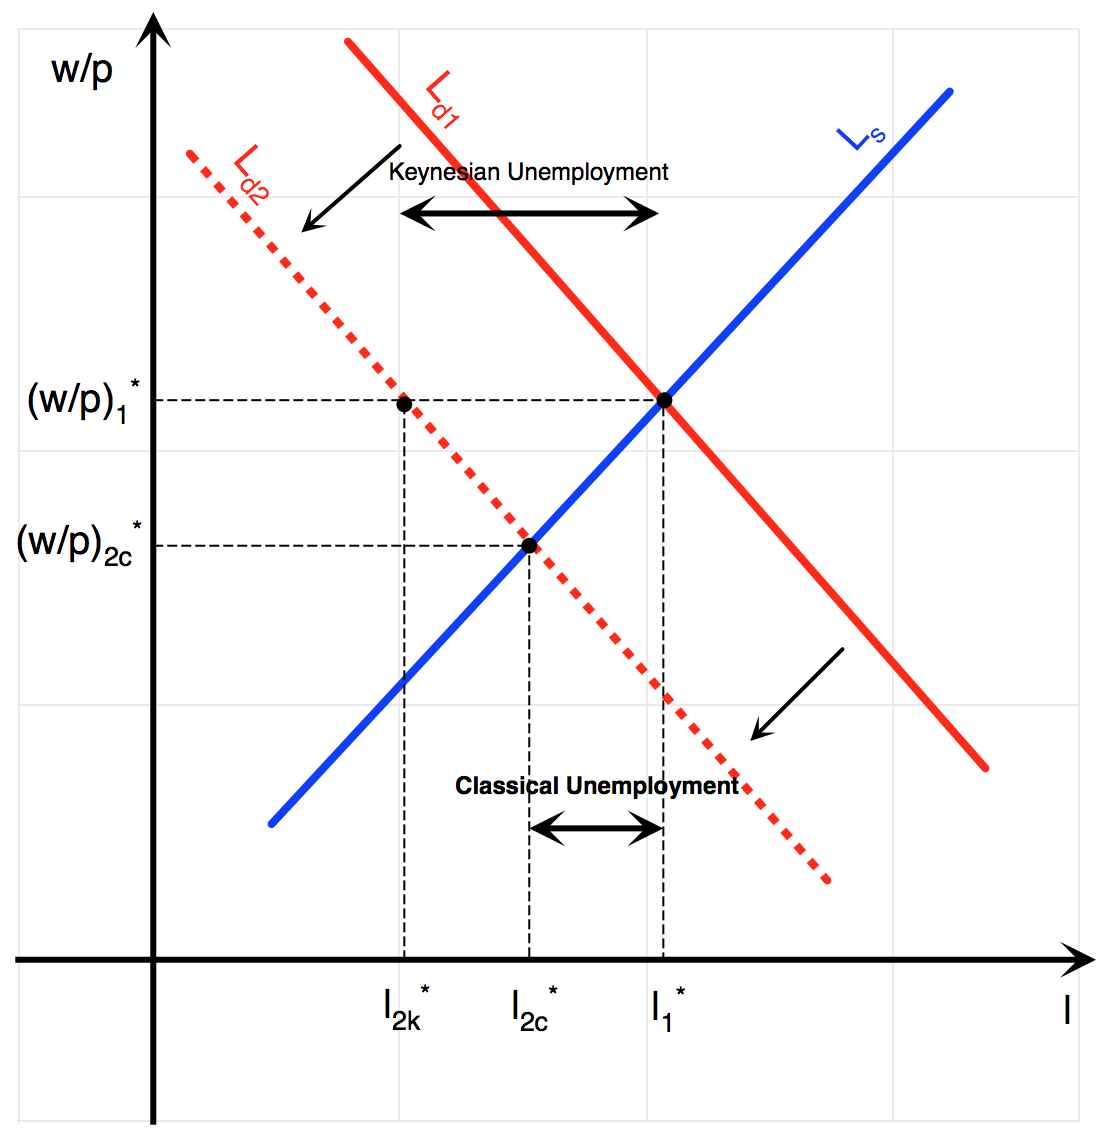
\includegraphics[width=0.75\linewidth]{graphsketcher/labor-market-productivity-shock-keynes} 

}

\caption{\textsc{Shock to Labor Demand in the
Neoclassical and ``Keynesian'' Models}.}\label{fig:shock-labor-demand}
\end{figure}

The graph shows clearly that ``Keynesian'' unemployment is larger than
Classical Unemployment: employment falls by more than if wages were
flexible.

Finally, I use quotes for ``Keynesian'' because although John Maynard
Keynes mentioned sticky wages in \emph{The General Theory of Employment,
Interest and Money} as a potential cause for unemployment, his thought
was much more complex, and he did not see a reduction in real wages as a
cure for unemployment. Although rigid wages have become synonymous with
Keynes' thought in many textbooks, you should keep in mind that John
Maynard Keynes' thought was much more complex than this, and that J.M.
Keynes actually was not in favor of a reduction in wages to cure
unemployment problems (you can see for yourself directly in
\href{http://cas2.umkc.edu/economics/people/facultypages/kregel/courses/econ645/winter2011/generaltheory.pdf}{The
General Theory}). If you want to know more, \emph{The Economist} has a
great briefing on the
\href{https://www.economist.com/economics-brief/2017/08/26/the-natural-rate-of-unemployment}{natural
rate of unemployment} - however, we will not investigate these notions
any further, so you are not responsible for the content of this article.

\hypertarget{bathtub}{\section{The Bathtub Model}\label{bathtub}}

A final view of unemployment consists in a mechanical, almost
statistical model of the labor market, called the ``bathtub'' model of
unemployment. This view recognizes that the labor market involves
constant churning, which implies that there always are some workers who
are in between jobs. It is called the bathtub model of unemployment
because in some ways, the unemployment rate is quite similar to the
height of the water in a bathtub.

\subsection{Model}\label{model-1}

In the bathtub model of unemployment, there is a number \(L\) of people
in the labor force. Jobs separate at a rate \(s\), often called the
\textbf{job separation rate}, and the rate at which unemployed people
find new jobs is \(f\), the \textbf{job finding rate}. For example,
assuming that in a typical month, 20\% of the unemployed find new jobs,
then \(f=20\)\%. If, on the other hand, 1\% of the employed lose their
jobs, then \(s=1\)\%. Finally, the number of people unemployed is
denoted by \(U_{t}\) and the number of people employed as \(E_{t}\). The
law of motion for the unemployment population is given by:
\[\Delta U_{t+1}=sE_{t}-fU_{t}.\]

\subsection{Solution}\label{solution-4}

Using the fact that people are either employed or unemployed:
\[E_{t}+U_{t}=L,\] and plugging in the law of motion for \(U_t\): \[
\begin{aligned}
\Delta U_{t+1}&=U_{t+1}-U_t=s\left(L-U_t\right)-fU_t\\
& \Rightarrow \quad U_{t+1}=(1-s-f)U_t+sL.
\end{aligned}
\] In the long run, we have that, the number of unemployed people
\(U^{*}\) satisfies the following equation:
\[U_{t+1}=U_{t}=U^{*}\quad\Rightarrow\quad U^{*}=\frac{sL}{s+f}.\]

The corresponding long run unemployment rate \(u^{*}\), that is the
number of unemployed as a function of the total population, is then
given by: \[u^{*}=\frac{U^{*}}{L}=\frac{s}{f+s}.\]

\textbf{Numerical Application.} Using the above numerical values, a job
separation rate of about \(s=1\)\%, as well as a job finding rate of
about \(f=20\)\%, we get a value for long-run unemployment, sometimes
called the natural rate of unemployment, equal to:
\[u^{*}=\frac{0.01}{0.2 + 0.01}\approx 4.8\%\].

\textbf{Transition dynamics.} Unlike with the Solow growth model of
\protect\hyperlink{solow}{lecture 2}, we can do more and ask how the
unemployment rate converges to this steady-state level, using the law of
motion for unemployment (this was impossible for the Solow growth model
because the law of motion for capital was too complex):

\[
\begin{aligned}
U_{t+1}&=\left(1-s-f\right)U_{t}+sL\\
& \quad\Rightarrow\quad U_{t+1}-U^{*}=\left(1-s-f\right)\left(U_{t}-U^{*}\right)\\
    & \quad\Rightarrow\quad U_{t}=U^{*}+\left(1-s-f\right)^{t}\left(U_{0}-U^{*}\right).
\end{aligned}
\]

\subsection{Data on Job Churning}\label{data-on-job-churning}

Data on job churning is collected by the Bureau of Labor Statistics (the
Job Opening and Labor Turnover Survey, also known as JOLTS). You may in
particular view the latest data on
\href{https://www.bls.gov/news.release/jolts.t01.htm}{Job openings},
\href{https://www.bls.gov/news.release/jolts.t02.htm}{Hires levels},
\href{https://www.bls.gov/news.release/jolts.t03.htm}{Total
separations},
\href{https://www.bls.gov/news.release/jolts.t04.htm}{Quits},
\href{https://www.bls.gov/news.release/jolts.t05.htm}{Layoffs and
discharges}.

The evolution of job openings and hire levels on the one hand, and total
separations, quits, layoffs and discharges are plotted on the two
figures below.

This data shows that there are many ways in which the bathtub model of
unemployment is an oversimplification. First, the separation and job
finding rates both fall substantially during recessions. Second, the
notion of a ``separation'' is a bit more subtle in the real world: some
separations are chosen from workers (quits), some of them are chosen by
firms (layoffs). Third, the job finding rate is also endogenous, because
not all job openings lead to hires.

Increased unemployment during recessions is explained by an increase in
layoffs, but more importantly by a decline in job openings.




\begin{figure}

{\centering 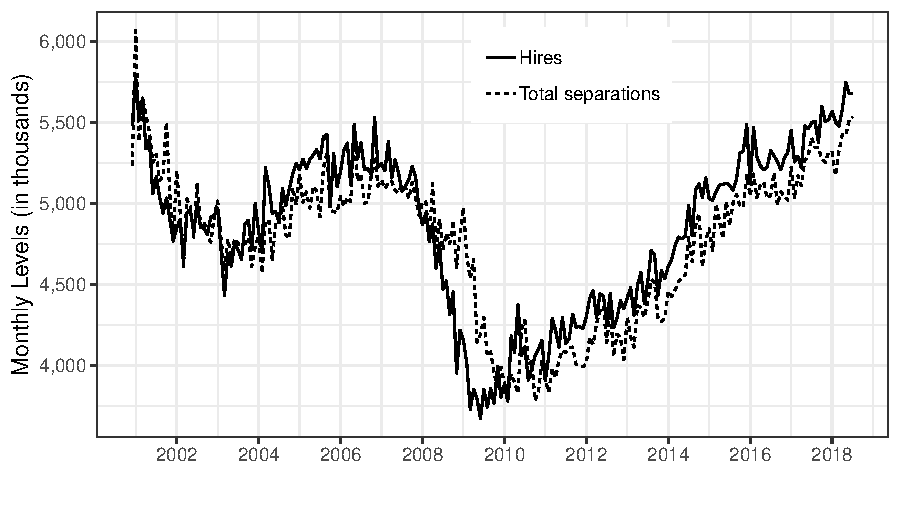
\includegraphics[width=1\linewidth]{ucla-102-fall2018_files/figure-latex/monthly-hires-1} 

}

\caption{\textsc{Monthly Hires and Separations, in Thousands.
Source: BLS-JOLTS}.}\label{fig:monthly-hires}
\end{figure}




\begin{figure}

{\centering 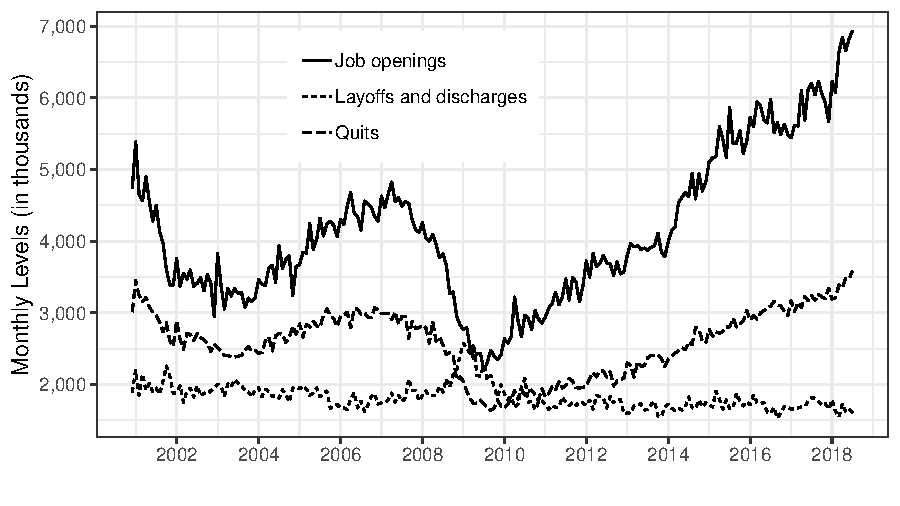
\includegraphics[width=1\linewidth]{ucla-102-fall2018_files/figure-latex/monthly-job-openings-1} 

}

\caption{\textsc{Monthly Job Openings, Layoffs and
Quits, in Thousands. Source: BLS-JOLTS}.}\label{fig:monthly-job-openings}
\end{figure}

\section*{Readings - To go further}\label{readings---to-go-further-3}
\addcontentsline{toc}{section}{Readings - To go further}

\href{https://www.economist.com/free-exchange/2011/01/17/several-quotes-in-search-of-a-theory}{Several
quotes in search of a theory, \emph{The Economist}, January 17, 2011.}

\href{https://doi.org/10.1111/1468-0297.00518}{Blanchard Olivier, and
Wolfers Justin. ``The Role of Shocks and Institutions in the Rise of
European Unemployment: The Aggregate Evidence.'' \emph{The Economic
Journal} 110, no. 462 (December 25, 2001): 1--33.}

\href{https://blogs.wsj.com/economics/2015/10/21/what-we-know-about-the-92-million-americans-who-arent-in-the-labor-force/}{What
We Know About the 92 Million Americans Who Aren't in the Labor Force,
\emph{Wall Street Journal}, Oct 21, 2015.}

(Gated)
\href{https://www.economist.com/economics-brief/2017/08/26/the-natural-rate-of-unemployment}{``Central
bankers' holy grail: The Natural rate of unemployment'', \emph{The
Economist}, August 26, 2017.}

\hypertarget{cons-function}{\chapter{The Consumption Function and the
Multiplier}\label{cons-function}}

This lecture opens a set of lectures on Keynesian economics. The
neoclassical models of consumption, saving, investment, and the labor
market that we have studied so far are quite close to what the
mainstream paradigm was teaching when John Maynard Keynes started to
think about these issues. J.M. Keynes refers to this paradigm as
``classical''. Yet, according to him, this paradigm was not a
\emph{general} one, in that it did not apply to a case where there was
an insufficient use of resources. According to him, the U.S. after the
Great Depression was in such a situation, where the teaching of
traditional economics was therefore ``misleading and disastrous''. The
first chapter of the
\href{http://cas2.umkc.edu/economics/people/facultypages/kregel/courses/econ645/winter2011/generaltheory.pdf}{General
Theory} starts with these words:

\begin{quote}
I have called this book the General Theory of Employment, Interest and
Money, placing the emphasis on the prefix general. The object of such a
title is to contrast the character of my arguments and conclusions with
those of the classical theory of the subject, upon which I was brought
up and which dominates the economic thought, both practical and
theoretical, of the governing and academic classes of this generation,
as it has for a hundred years past. I shall argue that the postulates of
the classical theory are applicable to a special case only and not to
the general case, the situation which it assumes being a limiting point
of the possible positions of equilibrium. Moreover, the characteristics
of the special case assumed by the classical theory happen not to be
those of the economic society in which we actually live, with the result
that its teaching is misleading and disastrous if we attempt to apply it
to the facts of experience.
\end{quote}

According to J.M. Keynes, the type of models we have seen so far are
\emph{special} in that they only apply in a case where there is full
employment of resources. In contrast, underutilization of resources
requires a different approach. In the model that we will study today,
consumption does not result from intertemporal optimization, as in
\protect\hyperlink{two-period}{Lecture 3} and
\protect\hyperlink{olg}{Lecture 4} but from a mechanical ``consumption
function'' relating consumption to current income. Investment is not be
determined by the supply of saving as in the Solow growth model of
\protect\hyperlink{solow}{Lecture 2}, but by the demand for investment
by firms. Finally, there may exist involuntary unemployment, unlike in
the neoclassical model of \protect\hyperlink{labor-market}{Lecture 6}.
Workers are potentially off their labor supply curve: they would be
willing to take a job at the current wage. In Keynes' view of the world,
an increase in demand can therefore potentially be met by an increase in
supply, because some labor is idle and ready to be used in production.

During this lecture, I first go through a presentation of the
\protect\hyperlink{simple}{simple Keynesian cross}, and then present a
couple of \protect\hyperlink{variations}{variations on the simple
Keynesian cross}: automatic stabilizers, and ``accelerator'' effects of
output on investment. The assumptions and logic of the Keynesian theory
may be a little disturbing at first:

\begin{quote}
The difficulty lies, not in the new ideas, but in escaping from the old
ones, which ramify, for those brought up as most of us have been, into
every corner of our minds.
\end{quote}

\section{The Demand for Goods}\label{the-demand-for-goods}

Consider the first accounting identity of
\protect\hyperlink{intro-cobb}{lecture 1}, showing the different
components of the demand for goods: \[Y=C+I+G+X-M.\] The total demand
for goods is determined by consumption demand, investment demand,
government spending, and net exports (for example, China's total demand
includes US' demand for Chinese products). For simplicity, we shall
assume for now that we are considering a closed economy - think, for
example, of the world economy - so that there are no exports or imports
(\(X=M=0\)). This assumption, which is not satisfying as the policies we
shall consider are national (fiscal policy, etc.), will be relaxed
starting in \protect\hyperlink{open}{lecture11}.

In \protect\hyperlink{solow}{lecture 2} and
\protect\hyperlink{olg}{lecture 4}, output was also determined by the
amount of available technology, as well as by the supply of labor \(L\),
and of capital \(K\) in the economy (the ``supply side''):
\[Y=F\left(K, L\right).\] For example, in the Solow growth model of
\protect\hyperlink{solow}{lecture 2}, where government spending was zero
(\(G=0\)), GDP was simultaneously equal to \(F(K,L)\) as well as to
\(C+I\). This is what allowed us to derive the dynamics in the economy.

In the Keynesian model, output is determined only by demand. The
underlying assumption is that there exists some idle resources which
allow to accommodate any increase in demand by an increase in labor
utilization. In order to show that output is determined by demand, we
shall denote the total demand for goods by \(Z\): \[Z=C+I+G.\] The
Keynesian assumption then is that output is demand determined, so that:
\[Y=Z.\] We now investigate these components of demand in turn.

\subsection{Consumption Demand}\label{consumption-demand}

The first (and largest) component of the demand for goods comes from
consumption. Rather than starting from microeconomic principles of
optimization under constraints, J.M. Keynes postulates a consumption
function relating disposable income to consumption. In its most general
form, consumption is simply a function of disposable income \(Y_D\),
disposable income being the income that remains once consumers have
received transfers from the government and paid their taxes:
\[C=C(Y_D), \quad \frac{dC}{dY_D}>0.\] The positive derivative implies
that when disposable income goes up, people buy more goods; when it goes
down, they buy fewer goods. It is often useful to specify a functional
form for this consumption function, such as: \[C(Y_D)=c_0+c_1Y_D.\] In
this case, the consumption function has a linear relation. This linear
relation has two parameters:

\begin{enumerate}
\def\labelenumi{\arabic{enumi}.}
\tightlist
\item
  \(c_1\) is called the \textbf{marginal propensity to consume}. It
  gives the effect of an additional dollar of income on consumption. For
  instance, if \(c_1=0.7\) (\(c_1=70\%\)), then an additional dollar of
  disposable income increases consumption by 1 dollar times 0.7, or 70
  cents. A natural restriction on \(c_1\) is that it is positive: an
  increase in disposable income should (at least averaging across
  individuals) lead to an increase in consumption. Another natural
  restriction on \(c_1\) is that it be less than \(1\): people are
  likely to save some of their increase in disposable income. Keynes
  presents this as follows in Chapter 10 of the
  \href{http://cas2.umkc.edu/economics/people/facultypages/kregel/courses/econ645/winter2011/generaltheory.pdf}{General
  Theory}:
\end{enumerate}

\begin{quote}
Our normal psychological law that, when the real income of the community
increases or decreases, its consumption will increase or decrease but
not so fast, can, therefore, be translated - not, indeed, with absolute
accuracy but subject to qualifications which are obvious and can easily
be stated in a formally complete fashion into the propositions that
\(\Delta C_w\) and \(\Delta Y_w\) have the same sign, but
\(\Delta Y_w > \Delta C_w\), where \(C_w\) is the consumption in terms
of wage-units. This is merely a repetition of the proposition already
established in Chapter 3 above. Let us define, then, \(dC_w/dY_w\) as
the marginal propensity to consume.
\end{quote}

\begin{enumerate}
\def\labelenumi{\arabic{enumi}.}
\setcounter{enumi}{1}
\tightlist
\item
  \(c_0\) corresponds to what people would consume if their disposable
  income was equal to \(0\) (for instance, they would still need to
  eat). In most instances, they would still be able to eat by running
  down their saving, or borrowing from banks. In terms of the model,
  changes in \(c_0\) should be thought of as everything that moves
  consumption without going through disposable income directly. This
  might therefore proxy for consumer confidence, the willingness of
  banks to lend to consumers, etc.
\end{enumerate}

Finally, disposable income is defined as: \[Y_D \equiv Y - T,\] where
\(Y\) is income and \(T\) is taxes paid minus government transfers
received by consumers. Very often, we will refer to \(T\) as ``taxes'',
which will always imply ``net taxes'', unless otherwise specified.

Finally, note that ``income'' includes here both labor income as well as
capital income, and is therefore equal to GDP. The underlying assumption
is that \(c_1\) represents a weighted average of marginal propensity to
consume across people with different incomes, and different types of
incomes.

\subsection{Investment Demand}\label{investment-demand}

The second component of the demand for goods is coming from investment
demand. In the Solow growth model, investment was determined by saving.
For the Keynesian model, we shall make two alternative assumptions about
investment:

\begin{enumerate}
\def\labelenumi{\arabic{enumi}.}
\item
  In the baseline version of the model, we shall assume that investment
  is fixed: \[I=\bar{I}.\] In order to remind ourselves that investment
  is fixed (or ``exogenous'', that is, determined outside of the model),
  we shall denote investment by ``I bar'' \(\bar{I}\).
\item
  In the investment accelerator version of the model, we shall assume in
  contrast that investment depends on output. This assumption is more
  realistic in practice: an Italian restaurant which has many customers
  is more likely to renovate it and to buy a new pizza oven. In this
  case, we will assume that investment depends on output in a linear
  way: \[I=b_0+b_1 Y.\]
\end{enumerate}

\subsection{Government Spending}\label{government-spending}

The third and final component of demand in our closed economy model is
government spending \(G\). Together with net taxes \(T\) representing
the tax-and-transfer system, \(G\) is a component of fiscal policy. We
shall also take \(G\) as exogenous, but we will study the impact of
alternative values for \(G\) for the determination of GDP, for example
(when we talk about the multiplier).

\hypertarget{simple}{\section{The Simple Goods Market
Model}\label{simple}}

The Simple Goods Market Model, also called the \textbf{(ZZ)-(YY) model},
assumes a closed economy, that investment is exogenous and equal to
\(\bar{I}\), an exogenous government spending \(G\), and a consumption
function given as above by: \[C=c_0+c_1\left(Y-T\right).\]

\subsection{Algebraic derivation of the
multiplier}\label{algebraic-derivation-of-the-multiplier}

\textbf{(ZZ) curve.} With these assumptions, and assuming a closed
economy, the value of the demand for goods \(Z\) is: \[
\begin{aligned}
Z   &=C+\bar{I}+G\\
    &=c_{0}+c_{1}\left(Y-T\right)+\bar{I}+G\\
Z   &=\left(c_{0}+\bar{I}+G-c_{1}T\right)+c_{1}Y
\end{aligned}
\] This determines a value for the demand for goods \(Z\), as a function
of aggregate income, or GDP \(Y\), which defines the (ZZ) curve. The
part of this demand which does not depend on income is called
\emph{autonomous spending} \(z_0\) defined as:
\[z_0=c_{0}+\bar{I}+G-c_{1}T.\] This autonomous spending \(z_0\) is also
the value of demand when income is equal to \(Y=0\). Therefore, the
demand for goods \(Z\) is given as:
\[Z=\underbrace{\left(c_{0}+\bar{I}+G-c_{1}T\right)}_{\text{Autonomous Spending }z_{0}}+\underbrace{c_{1}}_{\text{MPC}}Y\]

\textbf{(YY) curve.} Equilibrium in the goods market requires that:
\[Z=Y.\] Indeed, income is determined by the total demand for goods.

\textbf{Equilibrium.} Equilibrium is determined by the intersection of
the (YY) and the (ZZ) curves, represented by point A on the Figure
below. Replacing out \(Z=Y\) in the expression for \(Z\) above indeed
implies: \[Y=\left(c_{0}+\bar{I}+G-c_{1}T\right)+c_{1}Y.\] Therefore,
putting all \(Y\) terms of the left-hand side:
\[Y=\underbrace{\frac{1}{1-c_{1}}}_{\text{Multiplier}}\times\underbrace{\left(c_{0}+\bar{I}+G-c_{1}T\right)}_{\text{Autonomous Spending }z_{0}}.\]



\begin{figure}

{\centering 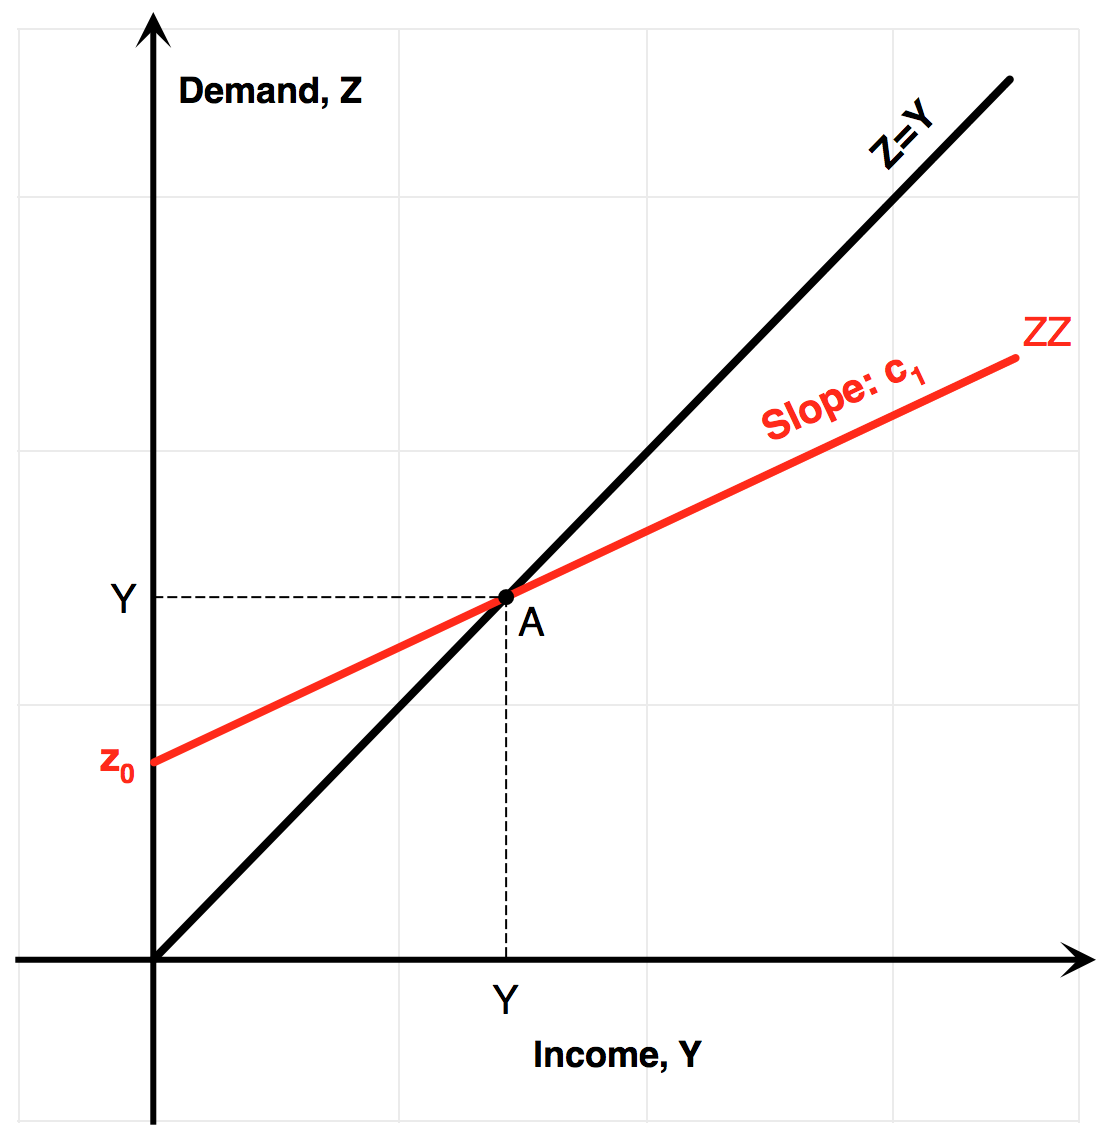
\includegraphics[width=0.5\linewidth]{graphsketcher/ZZ-YY} 

}

\caption{\textsc{The Simple Goods Market (ZZ)-(YY) model}.}\label{fig:zz-yy}
\end{figure}

\textbf{Multiplier.} Consider a change in autonomous spending
\(\Delta z_{0}=z_{0}'-z_{0}\) coming from a change in government
spending \(\Delta z_{0}=\Delta G\), or from a change in net taxes
\(\Delta z_{0}=-c_{1}\Delta T\). We have:
\[\Delta Y=\frac{\Delta z_{0}}{1-c_{1}}.\] By definition, the multiplier
gives the increase in income which is brought about by the increase in
autonomous spending. Therefore, the multiplier is given by:
\[\text{Multiplier}=\frac{1}{1-c_{1}}.\] As a consequence steepness of
the (ZZ) curve determines the value for the multiplier. The closer to
one the slope \(c_1\) is, the higher the value of the Keynesian
multiplier.

\textbf{Government expenditure multiplier; tax multiplier.} An increase
in government spending \(\Delta G>0\) leads to an increase in output
given by: \[\Delta Y=\frac{\Delta G}{1-c_{1}}.\] Thus, \(1/(1-c_1)\) is
usually called the \emph{government expenditure multiplier}.

On the other hand, a decrease in net taxes \(\Delta T<0\) leads to an
increase in output given by:
\[\Delta Y = - \frac{c_1 \Delta T}{1-c_{1}}.\] For this reason,
\(c_1/(1-c_1)\), or \(-c_1/(1-c_1)\) is sometimes called the tax
multiplier.

\subsection{Four interpretations}\label{four-interpretations}

Why is the change in output higher than the change in autonomous
spending? And why is it equal to \(1/(1-c_1)\), where \(c_1\) is the
marginal propensity to consume. There are actually four different ways
to see this, 2 are algebraic, and 2 are geometric:

\begin{enumerate}
\def\labelenumi{\arabic{enumi}.}
\item
  \textbf{Algebra.} The first way to see this is just, as above to
  equate output to demand \(Y=Z\), which allows to get at the result.
\item
  \textbf{Infinite sum of a geometric series.} 1\$ of additional
  autonomous spending brings in a second round \(c_{1}\)\$ increase in
  consumption, a third round \(c_{1}^{2}\)\$ increase in consumption,
  which add up to:
  \[\sum_{i=0}^{n}c_{1}^{i}=1+c_{1}+c_{1}^{2}+...+c_{1}^{n}=\frac{1-c_{1}^{n+1}}{1-c_{1}}.\]
  Therefore, because \(0<c_{1}<1\), we have:
  \[\text{Multiplier}=\sum_{i=0}^{+\infty}c_{1}^{i}=\frac{1}{1-c_{1}}.\]
\item
  \textbf{Graphical interpretation 1.} The left-hand panel of Figure
  \ref{fig:keynes-graphical} gives a graphical interpretation to this
  infinite geometric sum. This graphical interpretation makes it clear
  that: \[Y'-Y=\sum_{i=0}^{+\infty}c_{1}^{i}=\frac{1}{1-c_{1}}.\] This
  graph should make clear why the model is called a ``Keynesian cross''.
  This is because the (ZZ) and (YY) curves cross to determine output.
  This pedagogical device to visualize the Keynesian multiplier was
  introduced in 1948 by Paul Samuelson in his famous \emph{Economics}
  textbook, to provide a geometric intuitive interpretation of Keynes'
  ideas.
\end{enumerate}




\begin{figure}

{\centering 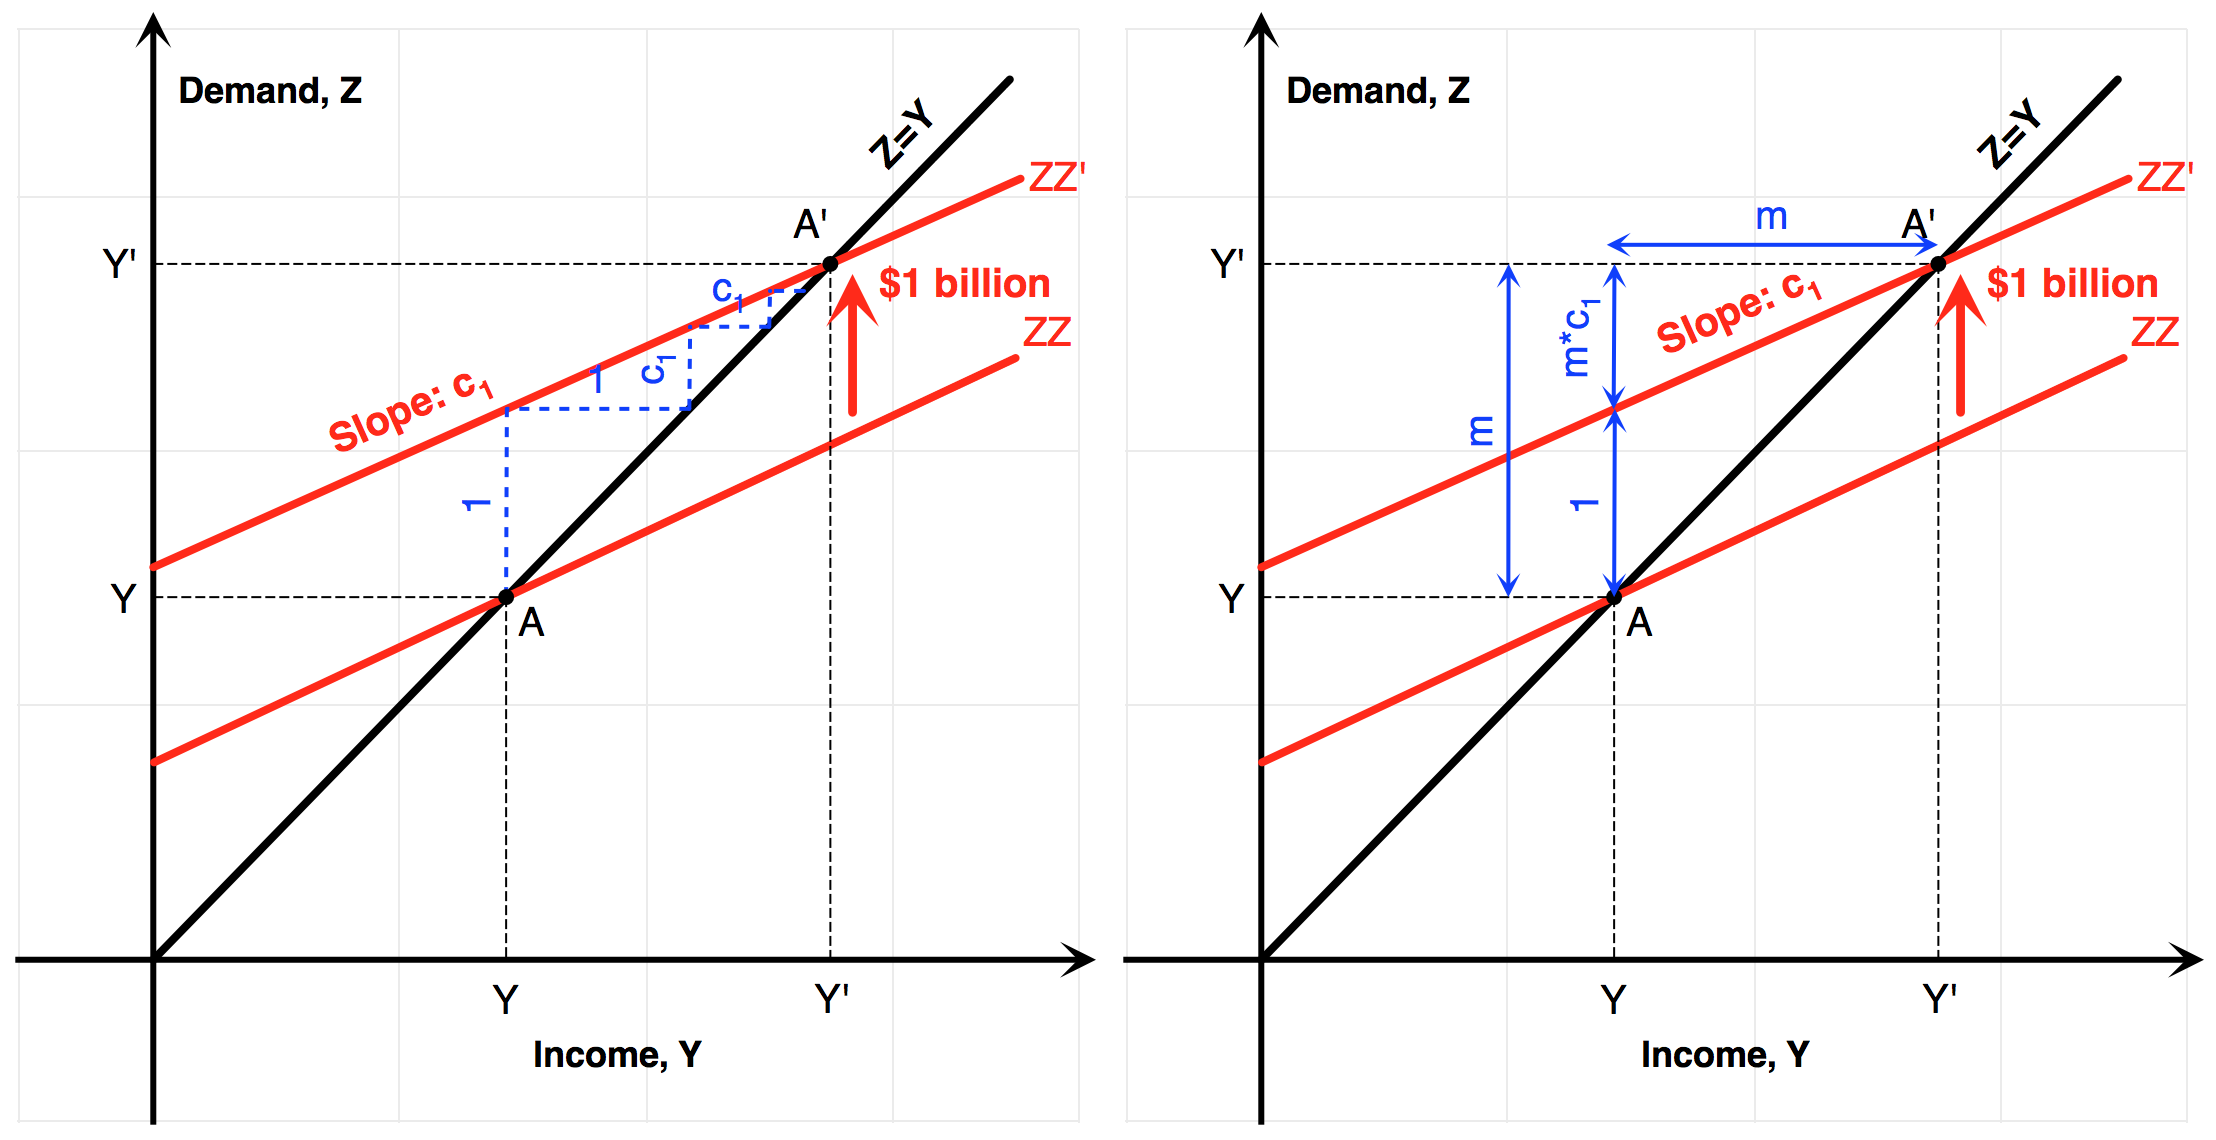
\includegraphics[width=1\linewidth]{graphsketcher/keynesian-cross-merged} 

}

\caption{\textsc{Simple Keynesian Cross: Graphical
Interpretations}.}\label{fig:keynes-graphical}
\end{figure}

\begin{enumerate}
\def\labelenumi{\arabic{enumi}.}
\setcounter{enumi}{3}
\tightlist
\item
  \textbf{Graphical interpretation 2.} The right-hand panel of Figure
  \ref{fig:keynes-graphical} gives a graphical interpretation which does
  not use a geometric sum. If \(m\) is the unknown value of the
  multiplier, then the geometry makes clear that \(m\) has to satisfy
  \(m=1+mc_{1}\) which also gives the value for the multiplier:
  \[m=1+mc_{1} \quad\Rightarrow\quad m=\frac{1}{1-c_{1}}.\]
\end{enumerate}

\hypertarget{variations}{\section{Extensions of the Goods Market
Model}\label{variations}}

There are multiple extensions of the Goods Market Model: one with
\protect\hyperlink{automatic}{automatic stabilizers}, one with an
\protect\hyperlink{accelerator}{accelerator effect of demand on
investment}.

\hypertarget{automatic}{\subsection{Automatic
Stabilizers}\label{automatic}}

In practice, the tax and transfer system is designed in such a way that
taxes strongly depend on the level of income: net taxes are said to be
\textbf{procyclical}:

\begin{enumerate}
\def\labelenumi{\arabic{enumi}.}
\item
  Many taxes, such taxes on wage income, profits, capital gains,
  mechanically collect more in revenues when income rises: taxes are
  procyclical (they vary positively with the state of the business
  cycle).
\item
  On the contrary, many transfers are countercyclical (they vary
  negatively with the state of the business cycle): when unemployment is
  high and income is low, more unemployment benefits or food stamps are
  being paid.
\end{enumerate}

Overall, these two effects reinforce themselves so that net taxes are
procyclical. In terms of the model, we model this by postulating a
linear function for net taxes which depends on the value for income:
\[T=t_{0}+t_{1}Y,\] where \(t_1 \in [0,1]\) indexes the cyclicality of
net taxes with GDP.

For example, assume that \(t_1=0.3\) or 30\%. Then if income rises by 1
dollar, net taxes rise by 30 cents. Using this expression for taxes
allows us to write: \[
\begin{aligned}
Z   &=C+\bar{I}+G\\
    &=c_{0}+c_{1}\left(Y-t_{0}-t_{1}Y\right)+\bar{I}+G\\
Z   &=\left(c_{0}-c_{1}t_{0}+\bar{I}+G\right)+\left(\left(1-t_{1}\right)c_{1}\right)Y
\end{aligned}
\] Using that \(Y=Z\) we see that the multiplier is now
\(1/(1-c_1(1-t_1))\):
\[Y=\frac{1}{1-c_{1}\left(1-t_{1}\right)}\left(c_{0}-c_{1}t_{0}+\bar{I}+G\right)\]
The (ZZ) curve is less steep, and therefore the multiplier \(Y'-Y\) is
smaller.




\begin{figure}

{\centering 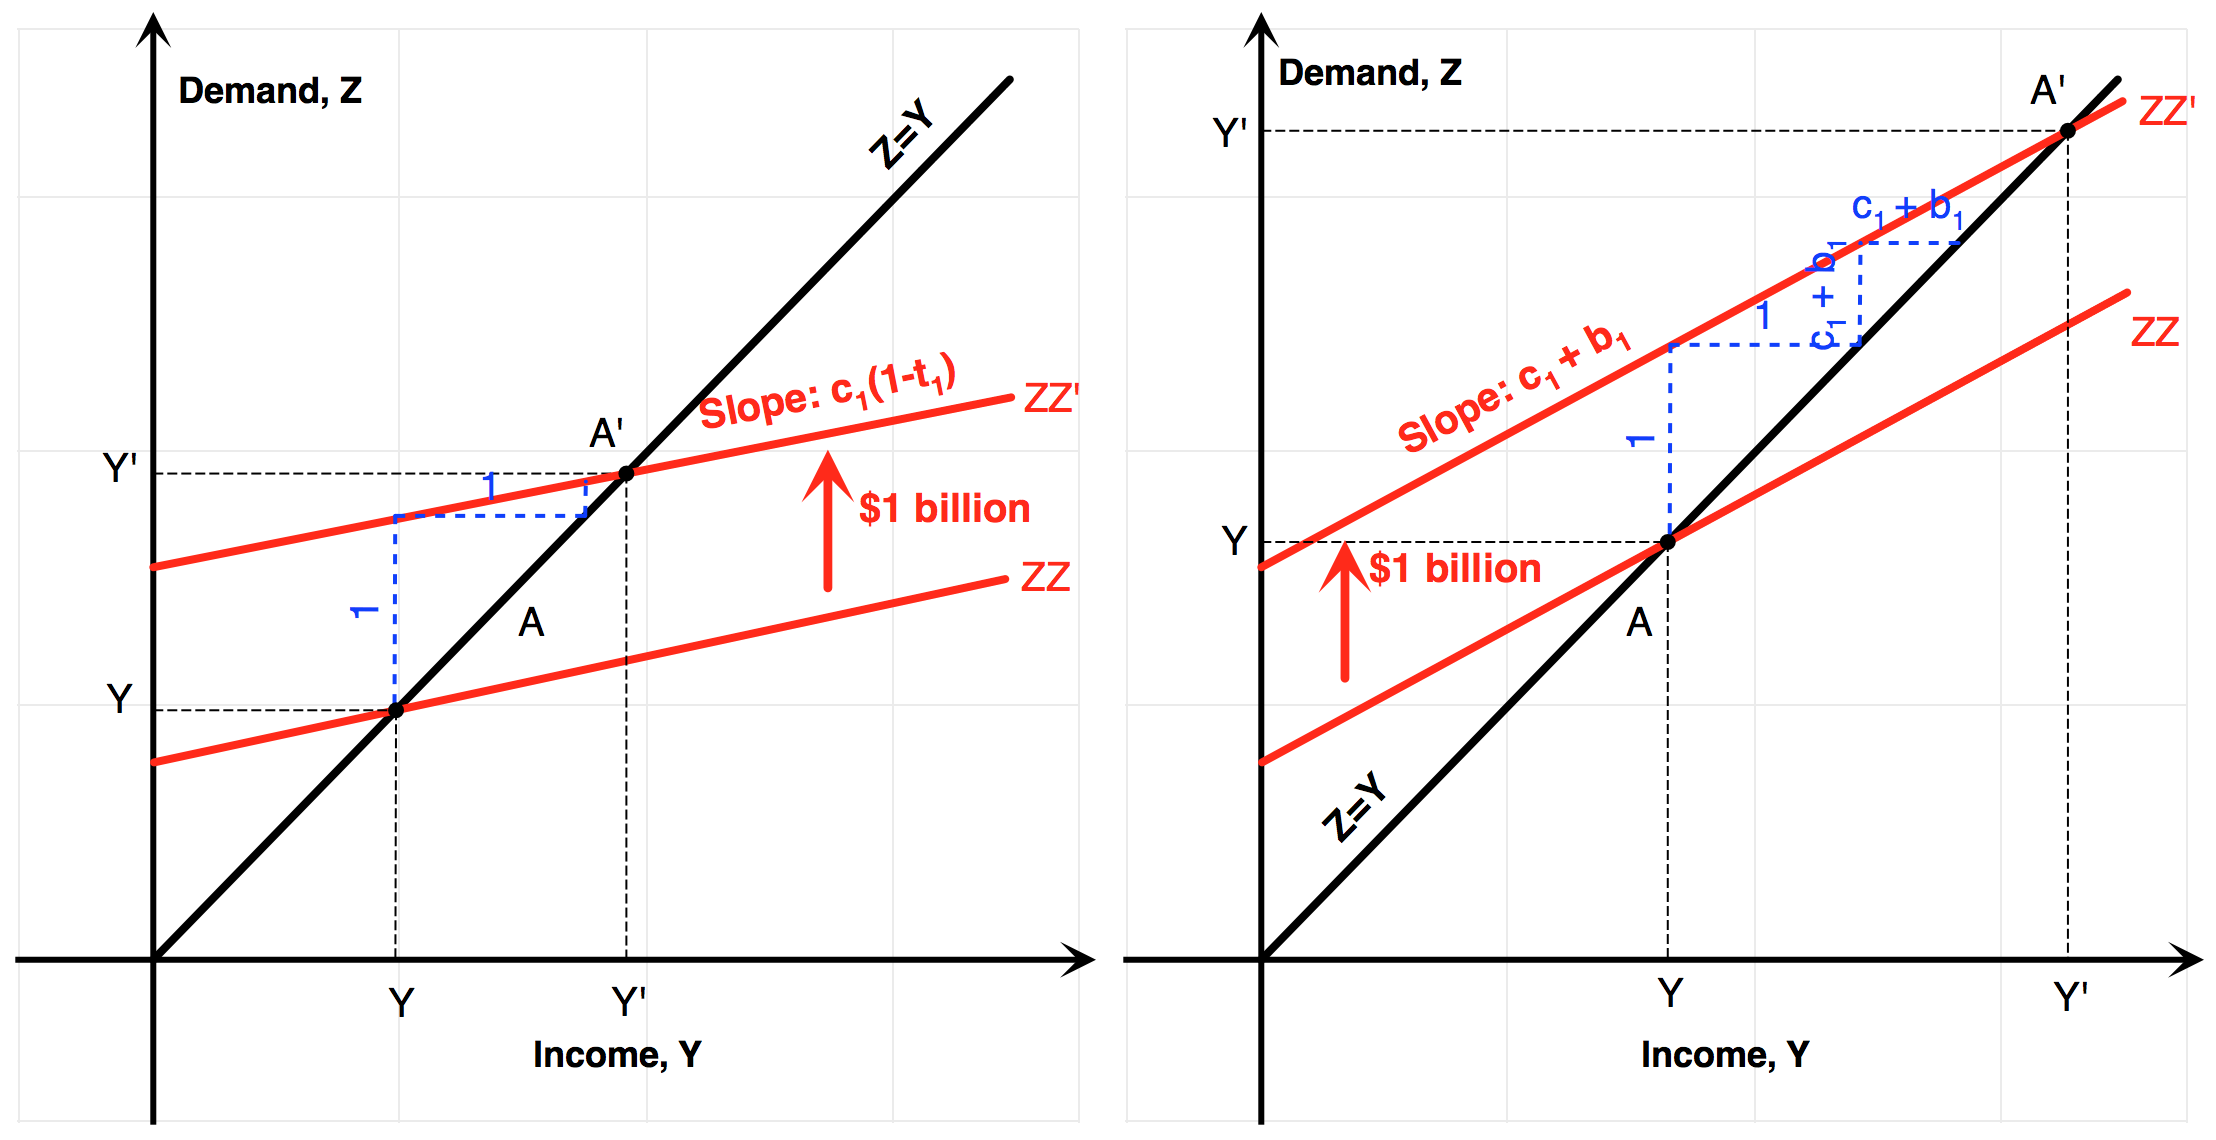
\includegraphics[width=1\linewidth]{graphsketcher/keynesian-cross-variations-merged} 

}

\caption{\textsc{Variations: Automatic Stabilizers,
Accelerator Effect}.}\label{fig:keynes-variations}
\end{figure}

\hypertarget{accelerator}{\subsection{\texorpdfstring{``Accelerator''
Effect}{Accelerator Effect}}\label{accelerator}}

Another variation on the Goods Market model consists in recognizing that
investment demand might also depend on income. Firms will invest more if
they expect high income, and therefore high demand for their goods:
\[I=b_{0}+b_{1}Y.\] Thus, the (ZZ)-curve now has a slope equal to
\(c_1+b_1\): \[
\begin{aligned}
Z   &=C+I+G\\
    &=c_{0}+c_{1}\left(Y-T\right)+b_{0}+b_{1}Y+G\\
Z   &=\left(c_{0}-c_{1}T+b_{0}+G\right)+\left(c_{1}+b_{1}\right)Y.
\end{aligned}
\] Using \(Z=Y\), we can conclude that the multiplier is
\(1/(1-c_1-b_1)\) if \(c_{1}+b_{1}<1\):
\[Y=\frac{1}{1-\left(c_{1}+b_{1}\right)}\left(c_{0}-c_{1}T+b_{0}+G\right)\]
In this case, the (ZZ) curve is steeper, and thus the multiplier
\(Y'-Y\) is larger. Note that if \(c_{1}+b_{1}\geq1\), then the
multiplier is infinite. This, of course, shows the limits of the
Keynesian model: it remains valid as long as output is constrained by
aggregate demand. In this case, output will increase to a level such as
it becomes constrained by supply, as in
\protect\hyperlink{solow}{lecture 2}.

\section*{Required Readings}\label{required-readings}
\addcontentsline{toc}{section}{Required Readings}

\href{https://search.proquest.com/docview/433963341/fulltext/43832006CCFE4D96PQ/1?accountid=14512}{Mankiw,
N. Gregory. What would Keynes have done? \emph{New York Times}, November
30, 2008}

\section*{Readings - To go further}\label{readings---to-go-further-4}
\addcontentsline{toc}{section}{Readings - To go further}

\href{https://socialsciences.mcmaster.ca/econ/ugcm/3ll3/keynes/pdf\%26filename\%3Dpeace3.pdf}{Keynes,
John Maynard. The Economic Consequences of the Peace, 1919.}

\href{https://cas2.umkc.edu/economics/people/facultypages/kregel/courses/econ645/winter2011/generaltheory.pdf}{Keynes,
John Maynard. Chapter 10 ``The Marginal Propensity to Consume and the
Multiplier'', The General Theory of Employment, Interest, and Money,
1936.}

\href{https://search.proquest.com/docview/398378701/fulltext/CBD1D9A468D04A85PQ/4?accountid=14512}{Robert
Barro. Keynes Is Still Dead. \emph{Wall Street Journal}. October 29,
1992.}

\href{https://www.forbes.com/2009/08/13/john-maynard-keynes-conservative-opinions-columnists-bruce-bartlett.html}{Bruce
Bartlett. Keynes Was Really A Conservative. \emph{Forbes}. August 14,
2009.}

\href{http://www.imf.org/external/pubs/ft/fandd/2014/09/pdf/basics.pdf}{What
Is Keynesian Economics?, \emph{Finance \& Development}, September 2014,
Sarwat Jahan, Ahmed Saber Mahmud, and Chris Papageorgiou.}

\hypertarget{paradox-thrift}{\chapter{The Paradox of
Thrift}\label{paradox-thrift}}

The idea that thrift is always virtuous is very deeply ingrained in our
culture. It is a matter of philosophy, morals, and sometimes even
religion. For example, in the
\href{https://www.youtube.com/watch?v=XxyB29bDbBA}{Walt Disney movie
Mary Poppins}, Michael is being lectured by a banker that he should not
be ``feeding the birds'' but instead invest his tuppence ``wisely in the
bank'' to ``be part of railways through Africa; Dams across the Nile,
fleets of ocean Greyhounds; Majestic, self-amortizing canals;
Plantations of ripening tea'' (interestingly, these capital investments
are all abroad; we shall come back to this later).

\begin{verbatim}
# [1] "Sorry I don't know how to embed videos in PDF: https://www.youtube.com/watch?v=XxyB29bDbBA"
\end{verbatim}

However, the model of \protect\hyperlink{cons-function}{lecture 7}
implies that saving might be detrimental to the economy, at least when
the economy has some slack. This phenomenon was explained by J.M. Keynes
in the
\href{http://cas2.umkc.edu/economics/people/facultypages/kregel/courses/econ645/winter2011/generaltheory.pdf}{\emph{General
Theory}}:

\begin{quote}
For although the amount of his own saving is unlikely to have any
significant influence on his own income, the reactions of the amount of
his consumption on the incomes of others makes it impossible for all
individuals simultaneously to save any given sums. Every such attempt to
save more by reducing consumption will so affect incomes that the
attempt necessarily defeats itself. It is, of course, just as impossible
for the community as a whole to save less than the amount of current
investment, since the attempt to do so will necessarily raise incomes to
a level at which the sums which individuals choose to save add up to a
figure exactly equal to the amount of investment.
\end{quote}

In this lecture, we use the models of
\protect\hyperlink{cons-function}{lecture 7} to understand that argument
better. From the outset, we should note that the paradox of thrift was
known before J.M. Keynes, perhaps in the
\href{https://en.wikipedia.org/wiki/Book_of_Proverbs}{Book of Proverbs}:

\begin{quote}
There is that scattereth, and yet increaseth; and there is that
withholdeth more than is meet, but it tendeth to poverty. (Proverbs
11:24)
\end{quote}

More certainly, it was present as early as in Bernard Mandeville's
\emph{The Fable of the Bees: or, Private Vices, Public Benefits} (1714):

\begin{quote}
As this prudent economy, which some people call Saving, is in private
families the most certain method to increase an estate, so some imagine
that, whether a country be barren or fruitful, the same method if
generally pursued (which they think practicable) will have the same
effect upon a whole nation, and that, for example, the English might be
much richer than they are, if they would be as frugal as some of their
neighbours. This, I think, is an error.
\end{quote}

This idea was also stated by Thomas Malthus:

\begin{quote}
Adam Smith has stated that capitals are increased by parsimony, that
every frugal man is a public benefactor, and that the increase of wealth
depends upon the balance of produce above consumption. That these
propositions are true to a great extent is perfectly
unquestionable\ldots{} But it is quite obvious that they are not true to
an indefinite extent, and that the principles of saving, pushed to
excess, would destroy the motive to production. If every person were
satisfied with the simplest food, the poorest clothing, and the meanest
houses, it is certain that no other sort of food, clothing, and lodging
would be in existence.
\end{quote}

\begin{quote}
While it is quite certain that an adequate passion for consumption may
fully keep up the proper proportion between supply and demand, whatever
may be the powers of production, it appears to be quite as certain that
a passion for accumulation must inevitably lead to a supply of
commodities beyond what the structure and habits of such a society will
permit to be consumed.
\end{quote}

Thomas Malthus really was a forerunner of J.M. Keynes. He set himself
out to explain why unemployment could occur, as well as to suggest steps
which might be taken to eliminate it. He was inspired by events
surrounding the post-Napoleonic wars period, during which time
industrial depression in Britain was causing serious unemployment of
labor and capital.

That this part of his thinking was not that original was in fact
recognized by J.M. Keynes in
\href{http://cas2.umkc.edu/economics/people/facultypages/kregel/courses/econ645/winter2011/generaltheory.pdf}{Chapter
23 of the General Theory - Notes on Mercantilism, the usury laws,
stamped money and theories of under-consumption}, which I strongly
encourage you to read (although you are not responsible for it). We will
come back to it when we talk about open economy macroeconomics, starting
in \protect\hyperlink{open}{lecture 11}

Back to our Keynesian goods market model of
\protect\hyperlink{cons-function}{lecture 7}, we shall now study the
paradox of thrift in more detail. We will consider three ways in which
an economy might save more, which are all relevant in practice:

\begin{enumerate}
\def\labelenumi{\arabic{enumi}.}
\item
  an increase in the desire to save through a fall in autonomous
  consumption \(\Delta c_0<0\).
\item
  an increase in public saving, also called \textbf{deficit reduction},
  through a decrease in government spending \(\Delta G<0\).
\item
  an increase in public saving, also called \textbf{deficit reduction},
  through an increase in taxes or a decrease in transfers
  \(\Delta T>0\).
\end{enumerate}

We will show that these acts of saving have very similar detrimental
effect on output, and therefore saving. We shall consider two models in
which such a paradox of thrift arises:

\begin{enumerate}
\def\labelenumi{\arabic{enumi}.}
\item
  in the \protect\hyperlink{simple}{simple goods market model} of
  \protect\hyperlink{cons-function}{lecture 7}, we will show that
  attempts to save more, either by private individuals or by the
  government, are self-defeating, in the sense that saving does not
  move.
\item
  in the \protect\hyperlink{extended}{variation on the goods market
  model} with an accelerator effect of investment where \(I=b_0+b_1Y\),
  we will even show that attemps to save more are more self-defeating:
  they lead to lower saving in the aggregate. The ``paradox of thrift''
  will appear very clearly: attempts to save more lead to less saving.
\end{enumerate}

\hypertarget{simple}{\section{Simple goods market model}\label{simple}}

Let us start from the simple goods market model: \[
\begin{aligned}
C   &=c_{0}+c_{1}Y_{D}\\
Y_{D}   &=Y-T,
\end{aligned}
\] where \(c_{1}\) is the marginal propensity to consume out of
disposable income \(Y_{D}\), disposable income is income minus taxes,
and investment \(I=\bar{I}\) and government spending \(G\) are taken as
given, as well as taxes \(T\). There are several ways to show the
``paradox of thrift'' in this model. We investigate an increase in the
desire to save, modeled as a reduction in \(c_0\) \(\Delta c_0<0\), as
well as two attempts at deficit reduction in turn.

\subsection{\texorpdfstring{\(\Delta c_{0}<0\)}{\textbackslash{}Delta c\_\{0\}\textless{}0}}\label{delta-c_00}

There are two ways to see that a fall in the desire to consume
\(\Delta c_0 <0\), or equivalently an increase in the desire to save,
may lead to an equal level of aggregate saving. One way is the most
straightforward, but does not give much intuition for the result. The
second way is more complex, but gives a very nice economic intuition.

\textbf{Direct proof.} The first way to see the paradox of thrift is
simply to notice that investment is fixed and equal to \(\bar{I}\) by
assumption. Since total saving equals private saving \(S\) plus public
saving \(T-G\), we can express private saving as a function of only
fixed variables:
\[\bar{I}=S+\left(T-G\right)\quad\Rightarrow\quad S=\bar{I}-\left(T-G\right).\]
This proves the result ! In particular, even if there is a change in
consumption of \(\Delta c_{0}<0\), then private saving does has to be
equal to \(\bar{I}-\left(T-G\right)\) always and thus cannot move.
However, this proof is a little bit disappointing and does not provide
much intuition.

\textbf{Intuitive Proof.} For the more intuitive proof, we need to write
the equations from the goods market model as well as equate output to
demand \(Y=Z\): \[\begin{aligned}
Y   =Z&=C+I+G\\
Y   &=c_{0}+c_{1}(Y-T)+\bar{I}+G
\end{aligned}\] This leads to equilibrium output:
\[Y=\frac{1}{1-c_{1}}\left(c_{0}-c_{1}T+\bar{I}+G\right).\]

This is the usual multiplier: for a given change in \(\Delta c_{0}\),
the change in output is given by the direct effect on output, but also
by all the successive new rounds, which add up to
\(\frac{\Delta c_{0}}{1-c_{1}}\) in total. Thus, such a change in
\(\Delta c_{0}\) leads to a change in output of:
\[\Delta Y=\frac{\Delta c_{0}}{1-c_{1}}.\]

Private saving is given by disposable income \(Y-T\) minus consumption
(what is earned, not paid in taxes, nor consumed, is saved), and
therefore:

\[
\begin{aligned}
S &= Y-T-C\\
&= Y-T-c_{0}-c_{1}\left(Y-T\right)\\
S   &= -c_{0}+\left(1-c_{1}\right)\left(Y-T\right).
\end{aligned}
\]

What happens when people attempt to save more, say by lowering
\(c_{0}\)? A change in consumption of \(\Delta c_{0}<0\) clearly leads
to:

\begin{itemize}
\item
  on the one hand, a \emph{direct effect} on private saving that is
  given by \(-\Delta c_{0}>0\) (private saving rises).
\item
  on the other hand, an \emph{indirect effect} going through the change
  in output whose magnitude was calculated above given by
  \(\Delta\left[\left(1-c_{1}\right)\left(Y-T\right)\right]\).
\end{itemize}

In other words, we may write:
\[\Delta S=\underbrace{\Delta(-c_{0})}_{\text{direct effect}}+\underbrace{\Delta\left[\left(1-c_{1}\right)\left(Y-T\right)\right]}_{\text{indirect effect}}.\]

Now, how large is the indirect effect? Some algebra allows to conclude
that it is exactly the opposite of the direct effect: \[\begin{aligned}
\Delta\left[\left(1-c_{1}\right)\left(Y-T\right)\right] &=(1-c_{1})\Delta Y\\
    &=(1-c_{1})\frac{\Delta c_{0}}{1-c_{1}}\\
\Delta\left[\left(1-c_{1}\right)\left(Y-T\right)\right] &=\Delta c_{0}.
\end{aligned}
\]

Therefore, the total effect on saving is: \[\begin{aligned}
\Delta S    &=\Delta(-c_{0})+\Delta\left[\left(1-c_{1}\right)\left(Y-T\right)\right]\\
    &=-\Delta c_{0}+\Delta c_{0}\\
\Delta S    &=0
\end{aligned}
\]

\subsection{\texorpdfstring{Fall in spending
\(\Delta G<0\)}{Fall in spending \textbackslash{}Delta G\textless{}0}}\label{fall-in-spending-delta-g0}

Again, there exists both a straightforward proof which does not explain
much, and a proof providing more economic intuition. We start with the
direct proof.

\textbf{Direct Proof.} The direct proof simply uses the investment
equals saving identity: \[\bar{I} = S + (T-G)\] This implies that a fall
in expenditure \(\Delta G<0\), and resulting increase in public saving
must be matched by a fall in private saving. However, this proof is
again, somewhat disappointing.

\textbf{Intuitive Proof.} Denote the fall in government spending by
\(\Delta G<0\). This leads to a rise in public saving:
\[\Delta(T-G)=-\Delta G>0.\] However, this fall also leads to a fall in
output, whose magnitude is given by the government spending multiplier.
Indeed, we know that:
\[Y=\frac{1}{1-c_{1}}\left(c_{0}-c_{1}T+\bar{I}+G\right),\] which
implies that the fall in output is:
\[\Delta Y=\frac{\Delta G}{1-c_{1}}.\]

Private saving is given by disposable income \(Y-T\) minus consumption
(what is earned, not paid in taxes, nor consumed, is saved), and
therefore: \[
\begin{aligned}
S   &= Y-T-C\\
&= Y-T-c_{0}-c_{1}\left(Y-T\right)\\
S   &=-c_{0}+\left(1-c_{1}\right)\left(Y-T\right).
\end{aligned}
\] Therefore: \[\Delta S=(1-c_{1})\Delta Y=\Delta G.\] Thus, we have a
fall in private saving whose magnitude is exactly matching the rise in
public saving. Overall, the effect on total saving, and therefore
investment is zero in this model: \[\Delta I  =\Delta S+\Delta(T-G)=0.\]

\subsection{\texorpdfstring{Increase in net taxes
\(\Delta T>0\)}{Increase in net taxes \textbackslash{}Delta T\textgreater{}0}}\label{increase-in-net-taxes-delta-t0}

An increase in net taxes \(\Delta T>0\) can come both from an increase
in taxes or a reduction in transfers. Again, there are two proofs. The
direct proof is exactly the same as the one with \(\Delta G<0\), so we
do not go over it. On the other hand, the intuitive proof is a bit
different because taxes impact disposable income too.

\textbf{Intuitive proof.} If the government chooses to engage in deficit
reduction through tax increases (or by reducing transfers), then
denoting by \(\Delta T>0\) the increase in aggregate taxes, we have a
rise in public saving given by: \(\Delta(T-G)=\Delta T>0\).

Again, this leads to a fall in private saving through two channels: a
direct channel which goes through the mechanic reduction in disposable
income, and a second channel which goes through the reduction in output,
which lowers income. Again, the magnitude of the second channel can be
computed using the above equation for output: \[
\begin{aligned}
&Y=\frac{1}{1-c_{1}}\left(c_{0}-c_{1}T+\bar{I}+G\right)\\
&\quad\Rightarrow\quad\Delta Y=-\frac{c_{1}}{1-c_{1}}\Delta T
\end{aligned}
\] Again, given the above expression for private saving:
\[S=-c_{0}+\left(1-c_{1}\right)\left(Y-T\right).\]

we have: \[
\begin{aligned}
\Delta S    &=(1-c_{1})(\Delta Y-\Delta T)\\
    &=(1-c_{1})\left(-\frac{c_{1}}{1-c_{1}}\Delta T\right)-(1-c_{1})\Delta T\\
\Delta S    &=\underbrace{-c_{1}\Delta T}_{\text{Effect through output}}-\underbrace{(1-c_{1})\Delta T}_{\text{Reduction in disposable income}}
\end{aligned}
\]

Therefore: \[\Delta S=-\Delta T.\]

Thus, we have a fall in private saving whose magnitude is exactly equal
to the rise in public saving. Overall, the effect on total saving, and
therefore investment is: \[\Delta I  =\Delta S+\Delta(T-G)=0.\]

\hypertarget{extended}{\section{Extended goods market
model}\label{extended}}

In the consumption and investment multiplier model, we get an even
stronger paradox of thrift in that efforts by consumers to save more
lead to declining saving. We thus start from the extended goods market
model of \protect\hyperlink{cons-function}{lecture 7}: \[
\begin{aligned}
C   &=c_{0}+c_{1}\left(Y-T\right)\\
I   &=b_{0}+b_{1}Y.
\end{aligned}
\] Again, we investigate a fall in private saving first, and then two
attempts at deficit reduction.

\subsection{\texorpdfstring{\(\Delta c_{0}<0\)}{\textbackslash{}Delta c\_\{0\}\textless{}0}}\label{delta-c_00-1}

\textbf{Direct proof.} Again, let us write the investment = total saving
identity:
\[I=S+\left(T-G\right)\quad\Rightarrow\quad S=I-\left(T-G\right).\] We
know that a fall in consumption of \(\Delta c_{0}<0\) leads to a decline
in output \(\Delta Y<0\), and therefore through the equation giving
investment as a function of output, to a decline in investment since
\(\Delta I=b_{1}\Delta Y\):
\[I=b_{0}+b_{1}Y\quad\Rightarrow\quad\Delta I=b_{1}\Delta Y.\] Because
\(T\) and \(G\) are assumed to be fixed (so that public saving is
fixed), the change in private saving is equal to the change in
investment, and is therefore negative. Therefore, a fall in consumption,
leads to a fall in private saving ! Again, that proof is probably not
very intuitive. We now turn to the longer proof.

\textbf{Intuitive proof.} Again, we write that output equals demand,
which allows to get an expression for output:
\[Y=\frac{1}{1-c_{1}-b_{1}}\left(c_{0}+b_{0}-c_{1}T+G\right)\] We have
the usual multiplier, compounding the consumption and investment effects
(it is assumed here that \(c_{1}+b_{1}<1\)). Therefore, a given change
in \(\Delta c_{0}<0\) leads to decline in output of:
\[\Delta Y=\frac{\Delta c_{0}}{1-c_{1}-b_{1}}.\] Again, one can show
that \(S=-c_{0}+\left(1-c_{1}\right)\left(Y-T\right)\) -- see
\protect\hyperlink{simple}{the previous section}:
\[\Delta S=\underbrace{\Delta(-c_{0})}_{\text{direct effect}}+\underbrace{\Delta\left[\left(1-c_{1}\right)\left(Y-T\right)\right]}_{\text{indirect effect}}\]
However, this time, the two effects do not exactly cancel out as the
indirect effect is: \[
\begin{aligned}
\Delta\left[\left(1-c_{1}\right)\left(Y-T\right)\right] &=(1-c_{1})\Delta Y\\
    &=(1-c_{1})\frac{\Delta c_{0}}{1-c_{1}-b_{1}}\\
\Delta\left[\left(1-c_{1}\right)\left(Y-T\right)\right] &=\frac{1-c_{1}}{1-c_{1}-b_{1}}\Delta c_{0}.
\end{aligned}
\] Therefore, the total effect on saving is negative: \[
\begin{aligned}
\Delta S    &=\Delta(-c_{0})+\Delta\left[\left(1-c_{1}\right)\left(Y-T\right)\right]\\
    &=-\Delta c_{0}+\frac{1-c_{1}}{1-c_{1}-b_{1}}\Delta c_{0}\\
\Delta S    &=\frac{b_{1}}{1-c_{1}-b_{1}}\Delta c_{0} <0
\end{aligned}
\]

\subsection{\texorpdfstring{Fall in spending
\(\Delta G<0\)}{Fall in spending \textbackslash{}Delta G\textless{}0}}\label{fall-in-spending-delta-g0-1}

\textbf{Direct proof.} We know that a rise in public saving, arising
from either a decrease in government spending, or a rise in taxes, or a
decrease in transfers, leads to a decline in output \(\Delta Y<0\), and
therefore through the above equation giving investment as a function of
output, to a decline in investment since \(\Delta I=b_{1}\Delta Y\):
\[I=b_{0}+b_{1}Y\quad\Rightarrow\quad\Delta I=b_{1}\Delta Y<0.\]
Therefore, a deficit reduction is clearly bad for investment. However,
once again, this calculation does not really help understand what the
above reasoning was wrong.

\textbf{Intuitive proof.} The fall in government spending \(\Delta G<0\)
leads to a rise in public saving: \[\Delta(T-G)=-\Delta G>0.\] However,
this fall also leads to a fall in output, whose magnitude is given by
the government spending multiplier. We write that output equals demand,
to get an expression for output to get, once again, that:
\[Y=\frac{1}{1-c_{1}-b_{1}}\left(c_{0}+b_{0}-c_{1}T+G\right)\] So the
fall in output is: \[\Delta Y=\frac{\Delta G}{1-c_{1}-b_{1}}.\] Once
again, private saving is given by disposable income \(Y-T\) minus
consumption (what is earned, not paid in taxes, nor consumed, is saved),
and therefore (see the previous sections):
\[S=-c_{0}+\left(1-c_{1}\right)\left(Y-T\right).\] Therefore:
\[\Delta S=(1-c_{1})\Delta Y=\frac{1-c_{1}}{1-c_{1}-b_{1}}\Delta G.\]
Thus, we have a fall in private saving whose magnitude is larger than
the rise in public saving. Overall, the effect on total saving, and
therefore investment is negative: \[
\begin{aligned}
\Delta I    &=\Delta S+\Delta(T-G)\\
&=\frac{1-c_{1}}{1-c_{1}-b_{1}}\Delta G-\Delta G\\
&=\frac{1-c_{1}}{1-c_{1}-b_{1}}\Delta G-\frac{1-c_{1}-b_{1}}{1-c_{1}-b_{1}}\Delta G\\
&=\frac{1-c_{1}-(1-c_{1}-b_{1})}{1-c_{1}-b_{1}}\Delta G\\
\Delta I &=\frac{b_{1}}{1-c_{1}-b_{1}}\Delta G<0.
\end{aligned}
\]

\subsection{\texorpdfstring{Increase in net taxes
\(\Delta T>0\)}{Increase in net taxes \textbackslash{}Delta T\textgreater{}0}}\label{increase-in-net-taxes-delta-t0-1}

The direct proof is exactly similar at the one in the previous section.
However, the intuitive proof is a bit difference.

\textbf{Intuitive proof.} If the government chooses to engage in deficit
reduction through tax increases (or by reducing transfers), then
denoting by \(\Delta T>0\) the increase in aggregate taxes, we have a
rise in public saving given by: \[\Delta(T-G)=\Delta T>0.\] Again, this
leads to a fall in private saving through two channels: a direct channel
which goes through the mechanic reduction in disposable income, and a
second channel which goes through the reduction in output, which lowers
income. Again, the magnitude of the second channel can be computed using
the above equation for output:
\[\Delta Y=-\frac{c_{1}}{1-c_{1}-b_{1}}\Delta T.\] Again, given the
above expression for private saving:
\[S=-c_{0}+\left(1-c_{1}\right)\left(Y-T\right).\] we have: \[
\begin{aligned}
\Delta S    &=(1-c_{1})(\Delta Y-\Delta T)\\
    &=(1-c_{1})\left(-\frac{c_{1}}{1-c_{1}-b_{1}}\Delta T\right)-(1-c_{1})\Delta T\\
\Delta S    &=\underbrace{-\frac{c_{1}(1-c_{1})}{1-c_{1}-b_{1}}\Delta T}_{\text{Effect through output}}-\underbrace{(1-c_{1})\Delta T}_{\text{Reduction in disposable income}}
\end{aligned}
\] Therefore:
\[\Delta S=-\frac{1-b_{1}-c_{1}+b_{1}c_{1}}{1-c_{1}-b_{1}}\Delta T.\]
Overall, the effect on total saving, and therefore investment is
decreasing:
\[\Delta I  =\Delta S+\Delta(T-G)=-\frac{b_{1}c_{1}}{1-c_{1}-b_{1}}\Delta T<0.\]

\section*{Readings - To go further}\label{readings---to-go-further-5}
\addcontentsline{toc}{section}{Readings - To go further}

\href{https://www.jstor.org/stable/1826621}{O'Leary, James J. ``Malthus
and Keynes.'' Journal of Political Economy 50, no. 6 (1942): 901--19.}

\href{https://en.wikipedia.org/wiki/Paradox_of_thrift}{Wikipedia,
Paradox of thrift.}

(Gated)
\href{https://krugman.blogs.nytimes.com/2009/07/07/the-paradox-of-thrift-for-real/}{Paul
Krugman, The Paradox of Thrift -- for real, \emph{New York Times}, July
7, 2008.}

\href{https://search.proquest.com/nytimes/docview/433945040/E76AA2F8F9C14A34PQ/2?accountid=14512}{Paul
Krugman, When Consumers Capitulate, \emph{New York Times}, October 31,
2008.}

\href{https://search.proquest.com/docview/399114897/CBD1D9A468D04A85PQ/2?accountid=14512}{Robert
J. Barro, Government Spending Is No Free Lunch, \emph{Wall Street
Journal}, January 22, 2009.}

\href{https://search.proquest.com/docview/1930920374/1A771BC8177A4FB7PQ/1?accountid=14512}{Paul
Krugman, A Dark Age of Macroeconomics (wonkish), \emph{New York Times},
Jan 27, 2009}

\href{https://search.proquest.com/docview/1930919033/3BCD850F469341AFPQ/1?accountid=14512}{Paul
Krugman, Paradox of Thrift, \emph{New York Times Blog}, February 3,
2009}

\href{https://search.proquest.com/nytimes/docview/1012047079/226EC4F8D3A49B0PQ/1?accountid=14512}{Robert
J. Barro, Stimulus Spending Keeps Failing; If austerity is so terrible,
how come Germany and Sweden have done so well?, \emph{Wall Street
Journal}, May 9, 2012.}

\href{https://search.proquest.com/docview/1020817739/fulltext/91FC1D36882C4B64PQ/1?accountid=14512}{Paul
Krugman, Greece As Victim, \emph{New York Times}, June 18, 2012.}

\hypertarget{redistributive}{\chapter{Redistributive
Policies}\label{redistributive}}

Keynesian economics provides a mechanism through which more
redistribution might actually increase output overall, at the same time
as it reduces inequality. The idea that the economy suffers from a
shortage of aggregate demand coming from increases in inequality has
been put forward recently by mainstream academics such as Raghuram
Rajan, former chief economist of the IMF, and now governor at the Bank
of England, as well as by Robert Reich, US Secretary of Labor from 1993
to 1997.

The idea that the MPC is influenced by the distribution of income and
wealth comes back to J.M. Keynes in the \emph{General Theory}:

\begin{quote}
Since the end of the nineteenth century significant progress towards the
removal of very great disparities of wealth and income has been achieved
through the instrument of direct taxation---income tax and surtax and
death duties---especially in Great Britain. Many people would wish to
see this process carried much further, but they are deterred by two
considerations; partly by the fear of making skilful evasions too much
worth while and also of diminishing unduly the motive towards
risk-taking, but mainly, I think, by the belief that the growth of
capital depends upon the strength of the motive towards individual
saving and that for a large proportion of this growth we are dependent
on the savings of the rich out of their superfluity. Our argument does
not affect the first of these considerations. But it may considerably
modify our attitude towards the second. For we have seen that, up to the
point where full employment prevails, the growth of capital depends not
at all on a low propensity to consume but is, on the contrary, held back
by it; and only in conditions of full employment is a low propensity to
consume conducive to the growth of capital. Moreover, experience
suggests that in existing conditions saving by institutions and through
sinking funds is more than adequate, and that measures for the
redistribution of incomes in a way likely to raise the propensity to
consume may prove positively favourable to the growth of capital.
\end{quote}

This passage from J.M. Keynes in the \emph{General Theory} is intuitive:
as long as saving propensities are no longer an impediment to capital
accumulation, redistributing income or wealth from low to high
\textbf{Marginal Propensity to Consume (MPC)} should lead to higher
output. According to J.M. Keynes, this is in fact one reason for
restricting the increase in inequality:

\begin{quote}
The State will have to exercise a guiding influence on the propensity to
consume partly through its scheme of taxation. (\ldots{}) Whilst,
therefore, the enlargement of the functions of government, involved in
the task of adjusting to one another the propensity to consume and the
inducement to invest, would seem to a nineteenth-century publicist or to
a contemporary American financier to be a terrific encroachment on
individualism, I defend it, on the contrary, both as the only
practicable means of avoiding the destruction of existing economic forms
in their entirety and as the condition of the successful functioning of
individual initiative.
\end{quote}

During this lecture, we derive this result using the Keynesian model
that was developed in \protect\hyperlink{cons-function}{lecture 7} and
\protect\hyperlink{paradox-of-thrift}{lecture 8}. One appeal of writing
the equations is that we are not able to prove these assertions
qualitatively, but we are also able to understand how important they are
quantitatively. As we go along, we therefore attempt to put some actual
numbers on all these arguments, to get a sense of the orders of
magnitude. We shall investigate two types of policies:

\begin{itemize}
\item
  Income redistribution, from high to low income earners.
\item
  Deficit-financed decreases in taxes, on high income earners or low
  income earners, financed by public debt.
\end{itemize}

\section{Assumptions}\label{assumptions-4}

Some minor modifications to the goods market model underlying
\protect\hyperlink{cons-function}{lecture 7} and
\protect\hyperlink{paradox-thrift}{lecture 8} are in order, in order to
think about stimulus policies in the presence of inequality. Instead of
assuming one type of consumer, with the average income \(Y\) and a given
MPC \(c_{1}\), we shall assume two types of workers. In total, there are
\(N\) workers:

\begin{itemize}
\item
  There is a fraction \(\lambda\) of low income earners, who earn income
  \(\underline{y}\), pay net taxes \(\underline{t}\), and the MPC of the
  low income earners is \(\underline{c}_{1}\):
  \[\underline{c}=\underline{c}_{0}+\underline{c}_{1}(\underline{y}-\underline{t}).\]
\item
  There is a fraction \(1-\lambda\) of high income earners, they get a
  higher income \(\bar{y}\) which is a multiple \(\gamma\) of low income
  earners' income, given by: \[\bar{y}=\gamma\underline{y},\] where
  \(\gamma\) indexes inequality. They each pay net taxes \(\bar{t}\),
  and the MPC of the high income earners is \(\bar{c}_{1}\):
  \[\bar{c}=\bar{c}_{0}+\bar{c}_{1}(\bar{y}-\bar{t})\] Moreover, we
  assume that high income earners have a lower MPC than low income
  earners, so that: \[\bar{c}_{1}<\underline{c}_{1}\]
\end{itemize}

We assume that investment depends on output: \[I=b_{0}+b_{1}Y\]

We also assume that taxes depend on output, both for low income earners:
\[\underline{t}=\underline{t}_{0}+t_1\underline{y}\] as well as for high
income earners: \[\bar{t}=\bar{t}_{0}+t_1\bar{y}.\]

\section{Solving the model}\label{solving-the-model}

\subsection{Income}\label{income}

Since there is a fraction \(\lambda\) of low income earners, and the
total population is \(N\), the total income \(\underline{Y}\) captured
by low income earners \(\underline{Y}\) is:
\[\underline{Y} = \lambda N \underline y\] Symmetrically, the total
income \(\bar{Y}\) captured by high income earners is:
\[\bar{Y}=(1-\lambda)N \bar{y}.\] Total income is given by the sum of
\(\underline{Y}\), and \(\bar{Y}\), which allows to express low income
earners as a function of total income: \[
\begin{aligned}
Y&=\underline{Y} + \bar{Y}\\
&=\lambda N \underline{y}+(1-\lambda) N \bar{y}\\
&=\lambda N \underline{y}+(1-\lambda) N \gamma\underline{y}\\
Y&=\left(\lambda +(1-\lambda)\gamma\right)N\underline{y}
\end{aligned}
\] This implies that low income earners' \(\underline{y}\) is given as a
function of output per person \(Y/N\) and the parameters of the model
by: \[\underline{y}=\frac{1}{\lambda+(1-\lambda)\gamma}\frac{Y}{N}\] As
a consequence, high income' individual \(\bar{y}\) is given as a
function of output per person \(Y/N\) and the parameters of the model
by:
\[\bar{y}=\gamma\underline{y}=\frac{\gamma}{\lambda+(1-\lambda)\gamma}\frac{Y}{N}.\]
The share of income captured by low income earners is: \[
\begin{aligned}
\frac{\underline{Y}}{Y}&=\frac{\lambda N \underline{y}}{\left(\lambda +(1-\lambda)\gamma\right)N\underline{y}}\\
\frac{\underline{Y}}{Y}&=\frac{\lambda}{\lambda +(1-\lambda)\gamma}.
\end{aligned}
\] The share of income captured by high income earners is: \[
\begin{aligned}
\frac{\bar{Y}}{Y}&=\frac{(1-\lambda) N \bar{y}}{\left(\lambda +(1-\lambda)\gamma\right)N\underline{y}}\\
&=\frac{(1-\lambda)\gamma N \underline{y}}{\left(\lambda +(1-\lambda)\gamma\right)N\underline{y}}\\
\frac{\bar{Y}}{Y}&=\frac{(1-\lambda)\gamma}{\lambda +(1-\lambda)\gamma}.
\end{aligned}
\]

\textbf{Numerical Application}: Approximate the number of workers in the
US to about 150 million: \[N = 150,000,000\] and that GDP is 20
trillion. Therefore, GDP per worker on average is:
\[\frac{Y}{N}=\$133,333.33\] Let us divide the population in two groups,
the top 10\% income share, and the bottom 90\% income share, so that:
\(\lambda = 0.9\). Since the top 10\% get approximately 50\% of the
income in the U.S. (the exact data is
\href{https://wid.world/world/\#sptinc_p90p100_z/US;FR;DE;CN;ZA;GB;WO/last/eu/k/p/yearly/s/false/25.253500000000003/80/curve/false/country}{available
here}), this implies, using the formula above
\(\underline{Y}/Y=\lambda/\left(\lambda +(1-\lambda)\gamma\right)\):
\[\frac{0.9}{0.9+0.1\cdot \gamma}=0.5 \quad \Rightarrow \quad \gamma = 9.\]
This is actually very intuitive: if 90\% of the population have the same
income as 10\% of the population (half of total income), then on average
they are 9 times poorer. The average income for someone in the top 10\%
is then:
\[\bar{y}=\gamma\underline{y}=\frac{\gamma}{\lambda+(1-\lambda)\gamma}\frac{Y}{N}=\$666,666.66\]
They are: \[(1-\lambda) N = 15,000,000.\] While the average income for
someone in the bottom 90\% is:
\[\underline{y}=\frac{1}{\lambda+(1-\lambda)\gamma}\frac{Y}{N}=\$74,074.07.\]
They are: \[\lambda N = 135,000,000.\]

\subsection{Taxes}\label{taxes}

Aggregate taxes \(T\) are the sum of taxes paid by the low income
earners \(\underline{T}\) and the high income earners \(\bar{T}\): \[
\begin{aligned}
T&=\underline{T} + \bar{T}\\
&=\lambda N \underline{t} + (1-\lambda) N \bar{t} \\
&=\lambda N \left(\underline{t}_{0}+t_1\underline{y}\right) + (1-\lambda) N \left(\bar{t}_{0}+t_1\bar{y}\right)\\
&=\left(\lambda N \underline{t}_{0} + (1-\lambda) N \bar{t}_{0}\right) + t_1\left(\lambda N \underline{y} + (1-\lambda)N\bar{y} \right)\\
T&=\left(\underline{T}_{0} + \bar{T}_{0}\right) + t_1 Y
\end{aligned}
\]

The aggregate baseline level of taxes \(T_0\) is:
\[T_{0} \equiv \underline{T}_0 +  \bar{T}_0 = \lambda  N \underline{t}_0 + (1-\lambda) N \bar{t}_0,\]
where baseline level of taxes for low and high income earners is given
by:
\[\underline{T}_0\equiv\lambda  N \underline{t}_0, \qquad \bar{T}_0\equiv(1-\lambda) N \bar{t}_0.\]
To conclude, total aggregate taxes are: \[
\begin{aligned}
\boxed{T=\left(\underline{T}_{0}+\bar{T}_{0}\right)+t_1 Y}.
\end{aligned}
\]

\subsection{Consumption}\label{consumption}

The challenging part, which differs from the models seen in
\protect\hyperlink{cons-function}{lecture 7} and
\protect\hyperlink{paradox-thrift}{lecture 8}, is to calculate aggregate
consumption, which is composed both of the consumption by low income
earners, and that by high income earners. Total consumption by the low
income earners \(\underline{C}\) is such that: \[
\begin{aligned}
\underline{C}&=\lambda N \underline{c}\\
&=\lambda N \left(\underline{c}_{0}+\underline{c}_{1}(\underline{y}-\underline{t})\right)\\
&=\lambda N  \underline{c}_{0} + \lambda N  (1-t_1) \underline{c}_{1}\underline{y}-\lambda N  \underline{c}_{1} \underline{t}_0\\
\underline{C}&=\left[\lambda N  \underline{c}_{0}-\lambda  N \underline{c}_{1} \underline{t}_0 \right]+ \frac{\lambda \underline{c}_{1}}{\lambda+(1-\lambda)\gamma}(1-t_1)Y
\end{aligned}
\]

Symmetrically, consumption by the high income earners \(\bar{C}\) is
such that: \[
\begin{aligned}
\bar{C}&=(1-\lambda) N \bar{c}\\
&=(1-\lambda) N \left(\bar{c}_{0}+\bar{c}_{1}(\bar{y}-\bar{t})\right)\\
&=(1-\lambda) N  \bar{c}_{0} + (1-\lambda) N (1-t_1) \bar{c}_{1}\bar{y}-(1-\lambda) N  \bar{c}_{1} \bar{t}_0\\
\bar{C}&=\left[(1-\lambda) N  \bar{c}_{0}-(1-\lambda) N  \bar{c}_{1} \bar{t}_0\right] + \frac{(1-\lambda) \gamma\bar{c}_{1}}{\lambda+(1-\lambda)\gamma}(1-t_1)Y
\end{aligned}
\]

Therefore, aggregate consumption \(C=\underline{C} + \bar{C}\) is given
by: \[
\begin{aligned}
C&=\underline{C} + \bar{C}\\
&=\left[\lambda N  \underline{c}_{0}-\lambda  N \underline{c}_{1} \underline{t}_0 \right]+ \frac{\lambda \underline{c}_{1}}{\lambda+(1-\lambda)\gamma}(1-t_1)Y + 
\left[(1-\lambda)  N \bar{c}_{0}-(1-\lambda) N  \bar{c}_{1} \bar{t}_0\right] + 
\frac{(1-\lambda) \gamma\bar{c}_{1}}{\lambda+(1-\lambda)\gamma}(1-t_1)Y\\
&=\left(\lambda N  \underline{c}_{0}+(1-\lambda) N  \bar{c}_{0}\right)-\left(\lambda  N \underline{c}_{1} \underline{t}_0 +(1-\lambda) N  \bar{c}_{1} \bar{t}_0\right) +\frac{\lambda\underline{c}_{1}+\left(1-\lambda\right)\gamma\bar{c}_{1}}{\lambda+(1-\lambda)\gamma}(1-t_1)Y\\
C&=C_0 -\left(\underline{c}_{1}\underline{T}_0+\bar{c}_{1}\bar{T}_0\right)+c_1 (1-t_1) Y.
\end{aligned}
\] where we have defined the average MPC \(c_1\) by:
\[c_{1}\equiv\frac{\lambda\underline{c}_{1}+\left(1-\lambda\right)\gamma\bar{c}_{1}}{\lambda+(1-\lambda)\gamma}.\]
the aggregate baseline level of consumption \(C_0\) as:
\[C_{0} \equiv \underline{C}_0 +  \bar{C}_0 = \lambda  N \underline{c}_0 + (1-\lambda) N \bar{c}_0,\]
where the baseline level of consumption for low and high income earners
is given by:
\[\underline{C}_0\equiv \lambda  N \underline{c}_0, \quad \bar{C}_0\equiv (1-\lambda) N \bar{c}_0.\]

To conclude, aggregate consumption is:
\[\boxed{C = C_0 -\left(\underline{c}_{1}\underline{T}_0+\bar{c}_{1}\bar{T}_0\right)+c_1 (1-t_1) Y}.\]

\section{Aggregate Demand}\label{aggregate-demand}

We want to compute aggregate demand: \[Z=C+I+G.\] We know that \(I\) has
a very straightforward expression: \[I=b_0 +b_1 Y.\] Using the
expression for aggregate consumption \(C\) as well and plugging in into
total demand yields: \[
\begin{aligned}
Z   &=C+I+G\\
    &=C_0 -\left(\underline{c}_{1}\underline{T}_0+\bar{c}_{1}\bar{T}_0\right)+c_1 (1-t_1) Y + b_{0}+b_{1}Y+G\\
Z   &=\left[C_0 -\left(\underline{c}_{1}\underline{T}_0+\bar{c}_{1}\bar{T}_0\right)+ b_{0} + G \right]+ \left(c_1(1-t_1) + b_1\right) Y 
\end{aligned}
\]

Equating output to demand \(Z = Y\) gives the value for output:
\[\boxed{Y=\frac{1}{1-\left(1-t_{1}\right)c_{1}-b_{1}}\left[C_0-\underline{c}_{1}\underline{T}_{0}-\bar{c}_{1}\bar{T}_{0}+b_{0}+G\right]}\]

\section{Different Fiscal Policies}\label{different-fiscal-policies}

\subsection{Redistribution from high income to low income
earners}\label{redistribution-from-high-income-to-low-income-earners}

Assume that transfers to the low income earners are increased (or taxes
decreased), so that \(\Delta\underline{T}_{0}<0\), with an offsetting
increase in taxes on high income earners such that
\(\Delta T_0 = \Delta\underline{T}_{0}+\Delta\bar{T}_{0}=0\). We then
have that \(\Delta\bar{T}_{0}=-\Delta\underline{T}_{0}>0\). This leads
to a change in autonomous spending:
\[\Delta z_{0}=-\underline{c}_{1}\Delta\underline{T}_{0}-\bar{c}_{1}\Delta\bar{T}_{0}\quad\Rightarrow\quad\Delta z_{0}=\left(\underline{c}_{1}-\bar{c}_{1}\right)\Delta\bar{T}_{0}>0.\]

That impulse leads to an increase in output given by:
\[\Delta Y=\frac{\underline{c}_{1}-\bar{c}_{1}}{1-\left(1-t_{1}\right)c_{1}-b_{1}}\Delta\bar{T}_{0}>0.\]

Using the value for aggregate taxes: \[
\begin{aligned}
&T=\left(\underline{T}_{0}+\bar{T}_{0}\right)+t_1 Y\\
&\quad \Rightarrow \quad \Delta T=\underbrace{\Delta\underline{T}_{0}+\Delta\bar{T}_{0}}_{\Delta T_0 = 0}+t_1\Delta Y.
\end{aligned}
\] Finally:
\[\Delta T=\frac{t_1\left(\underline{c}_{1}-\bar{c}_{1}\right)}{1-\left(1-t_{1}\right)c_{1}-b_{1}}\Delta\bar{T}_{0}.\]

Thus, public saving increase, there is a reduction in the deficit, in
public debt, and therefore:
\[\Delta\left(T-G\right)=\frac{t_1\left(\underline{c}_{1}-\bar{c}_{1}\right)}{1-\left(1-t_{1}\right)c_{1}-b_{1}}\Delta\bar{T}_{0}\]

\textbf{Numerical Application}: On top of the above numerical values, we
assume that the marginal tax rate is 25\% so that \(t_1=1/4\).
Therefore:
\[\underline{c}_{1}=1, \quad \bar{c}_{1}=1/3,\quad \gamma=9, \quad\lambda=0.9,\quad b_1=1/6, \quad t_1=1/4.\]
As shown above, this implies an average MPC given by \(c_1=2/3.\) Thus,
a tax cut to low income earners financed by tax increases to high income
earners leads to an increase in output given by the following
multiplier: \[
\begin{aligned}
\frac{\underline{c}_{1}-\bar{c}_{1}}{1-(1-t_1)c_{1}-b_{1}} &= \frac{1-1/3}{1-(1-1/4)*2/3-1/6}\\
&= \frac{2/3}{1-1/2-1/6}\\
\frac{\underline{c}_{1}-\bar{c}_{1}}{1-(1-t_1)c_{1}-b_{1}} &=2
\end{aligned}
\] This implies that if \$1 billion is transfered from high to low
income earners, GDP rises by \$2 billion. Importantly, this does not
necessarily imply it should be done: first, high income earners are
clearly worse off. Second, this calculation based on high income
earners' lower MPC does not take into account that they may be
discouraged to create jobs and become entrepreneurs if they are taxed
too much.

Because output increases, we get an improvement in the budget surplus as
well, given by: \[
\begin{aligned}
\Delta\left(T-G\right)&=t_1*\frac{\left(\underline{c}_{1}-\bar{c}_{1}\right)}{1-\left(1-t_{1}\right)c_{1}-b_{1}}*\Delta\bar{T}_{0}\\
&=\frac{1}{4}*2*1\\
\Delta\left(T-G\right)&=\frac{1}{2}
\end{aligned}
\] or, 500 million dollar improvement.

Therefore, \textbf{\$1 billion dollar transfer from high to low income
earners} leads to an improvement in the public \textbf{surplus} of
\textbf{\$0.5 billion dollars}.

\subsection{Deficit-financed tax cuts for high income
earners}\label{deficit-financed-tax-cuts-for-high-income-earners}

Assume tax cuts for high income earners \(\Delta\bar{T}_{0}<0\), then
output increases:
\[\Delta Y=-\frac{\bar{c}_{1}}{1-\left(1-t_{1}\right)c_{1}-b_{1}}\Delta\bar{T}_{0}>0\]

The impact on aggregate taxes is however ambiguous: \[
\begin{aligned}
\Delta T    &=\Delta\bar{T}_{0}+\underbrace{\Delta\underline{T}_{0}}_{=0}+t_1\Delta Y\\
\Delta T    &=\left(1-\frac{t_1\bar{c}_{1}}{1-\left(1-t_{1}\right)c_{1}-b_{1}}\right)\Delta\bar{T}_{0}
\end{aligned}
\]

Therefore, the impact on public saving is similarly ambiguous:
\[\Delta\left(T-G\right)=\left(1-\frac{t_1\bar{c}_{1}}{1-\left(1-t_{1}\right)c_{1}-b_{1}}\right)\Delta\bar{T}_{0}\]

There is an increase in output and, depending on parameters, there can
be a government surplus or a government deficit.

\textbf{Numerical Application}: We assume:
\[\underline{c}_{1}=1, \quad \bar{c}_{1}=1/3,\quad \gamma=9, \quad\lambda=0.9,\quad b_1=1/6, \quad t_1=1/4.\]
This implies \(c_1=2/3.\) Thus, we may calculate the tax multiplier for
tax cuts to high income earners, which is given by: \[
\begin{aligned}
\frac{\bar{c}_{1}}{1-(1-t_1)c_{1}-b_{1}} &= \frac{1/3}{1-(1-1/4)*2/3-1/6}\\
&= \frac{1/3}{1-1/2-1/6}\\
\frac{\bar{c}_{1}}{1-(1-t_1)c_{1}-b_{1}} &=1
\end{aligned}
\]

Therefore, the impact on public saving is given by: \[
\begin{aligned}
\Delta\left(T-G\right)&=\left(1-\frac{t_1\bar{c}_{1}}{1-\left(1-t_{1}\right)c_{1}-b_{1}}\right)\Delta\bar{T}_{0}\\
&=\left(1-t_1*\frac{\bar{c}_{1}}{1-\left(1-t_{1}\right)c_{1}-b_{1}}\right)\Delta\bar{T}_{0}\\
&=\left(1-\frac{1}{4}*1\right)*(-1)\\
\Delta\left(T-G\right)&=-\frac{3}{4}
\end{aligned}
\] Therefore, \textbf{\$1 billion dollar tax cut on high income earners}
leads to an increase in the public \textbf{deficit} of \textbf{\$0.75
billion dollars}.

\subsection{Deficit-financed tax cuts for low income
earners}\label{deficit-financed-tax-cuts-for-low-income-earners}

Assume tax cuts for low income earners \(\Delta\underline{T}_{0}<0\),
then output increases:
\[\Delta Y=-\frac{\underline{c}_{1}}{1-\left(1-t_{1}\right)c_{1}-b_{1}}\Delta\underline{T}_{0}>0.\]

The impact on aggregate taxes is however ambiguous: \[
\begin{aligned}
\Delta T    &=\Delta\underline{T}_{0}+\underbrace{\Delta\bar{T}_{0}}_{=0}+t_1\Delta Y\\
\Delta T    &=\left(1-\frac{t_1\underline{c}_{1}}{1-\left(1-t_{1}\right)c_{1}-b_{1}}\right)\Delta\underline{T}_{0}
\end{aligned}
\]

The impact on public saving is similarly ambiguous:
\[\Delta\left(T-G\right)=\left(1-\frac{t_1\underline{c}_{1}}{1-\left(1-t_{1}\right)c_{1}-b_{1}}\right)\Delta\underline{T}_{0}\]

There is an increase in output and, depending on parameters, there can
be a government surplus or a government deficit.

\textbf{Numerical Application}: We assume:
\[\underline{c}_{1}=1, \quad \bar{c}_{1}=1/3,\quad \gamma=9, \quad\lambda=0.9,\quad b_1=1/6, \quad t_1=1/4.\]
This implies \(c_1=2/3.\) Thus, we may calculate the tax multiplier for
tax cuts to low income earners, which is given by: \[
\begin{aligned}
\frac{\underline{c}_{1}}{1-(1-t_1)c_{1}-b_{1}} &= \frac{1}{1-(1-1/4)*2/3-1/6}\\
&= \frac{1}{1-1/2-1/6}\\
\frac{\underline{c}_{1}}{1-(1-t_1)c_{1}-b_{1}} &=3
\end{aligned}
\]

Therefore, the impact on public saving is given by: \[
\begin{aligned}
\Delta\left(T-G\right)&=\left(1-\frac{t_1\underline{c}_{1}}{1-\left(1-t_{1}\right)c_{1}-b_{1}}\right)\Delta\underline{T}_{0}\\
&=\left(1-t_1*\frac{\underline{c}_{1}}{1-\left(1-t_{1}\right)c_{1}-b_{1}}\right)\Delta\underline{T}_{0}\\
&=\left(1-\frac{1}{4}*3\right)*(-1)\\
\Delta\left(T-G\right)&=-\frac{1}{4}
\end{aligned}
\] Therefore, \textbf{\$1 billion dollar tax cut on low income earners}
leads to an increase in the public \textbf{deficit} of \textbf{\$0.25
billion dollars}.

\section*{Readings - To go further}\label{readings---to-go-further-6}
\addcontentsline{toc}{section}{Readings - To go further}

\href{https://krugman.blogs.nytimes.com/2013/11/16/secular-stagnation-coalmines-bubbles-and-larry-summers/}{``Secular
Stagnation, Coalmines, Bubbles, and Larry Summers'', Paul Krugman,
\emph{New York Times} Blog Post, November 16, 2013.}

\href{https://search.proquest.com/docview/1473347330/6C9B371C00BE4C7BPQ/1?accountid=14512}{``The
Economic Hokum of `Secular Stagnation'\,'', John B. Taylor, \emph{Wall
Street Journal}, January 2, 2014.}

\href{http://larrysummers.com/2016/02/17/the-age-of-secular-stagnation/}{``The
Age of Secular Stagnation'', Larry Summers, \emph{Foreign Affairs},
February 15, 2016.}

\href{https://www.epi.org/publication/secular-stagnation/}{``Inequality
Is Slowing US Economic Growth: Faster Wage Growth for Low- and
Middle-Wage Workers Is the Solution'', Josh Bivens, Economic Policy
Institute, December 12, 2017.}

\hypertarget{public-debt}{\chapter{Public Debt, Say's
Law}\label{public-debt}}

Until now, we have been talking about government spending and taxes as
if the government could take on as much debt as it wants. But then, why
doesn't the government just engage in more tax cutting and more
government spending, or both? We alluded to a first reason when we
talked about the consequences of having \(1-c_1<b_1\), or the propensity
to save be less than the propensity to invest. We argued then that we
would never be in a Keynesian situation of deficient aggregate demand,
so that multiplier effects would stop when facing constraints on supply.
Similarly, if the government started to make public saving very negative
(running a budget deficit), then it would similarly start facing
constraints on what the economy can supply. For instance, if fiscal
policy was too accommodative, and to the limit if \(G\) was set at too
high a value, then supply constraints would start to bite: one example
was given historically in the 1940s when the U.S. engaged in World War
II. However, these levels of spending are clearly out of the question,
and this is perhaps not what constrains the government from doing a
little bit more spending, or a little bit more tax reductions.

Another potentially more pressing issue is that of the government
deficit, and the impact of government debt on future generations. The
Trump tax cuts which have just been enacted have reduced unemployment to
historically low levels, and pushed GDP growth up to a level which has
not been seen in a long time, as predicted by the Keynesian model;
however, it also has raised U.S. public debt, and is being criticized
mostly on these grounds. This makes sense: when government spending
increases \(\Delta G>0\), this leads to a government deficit of equal
magnitude: \(\Delta (T-G) = -\Delta G<0.\) Similarly, a tax cut
\(\Delta T<0\) leads to increased deficits given by
\(\Delta (T-G) = \Delta T<0\) \footnote{Note however that automatic
  stabilizers go against that: in \href{pset6.html}{problem set 6}, we
  even saw that tax cuts sometimes can pay for themselves. However, this
  happens only if the multiplier is really very high. For example, if
  tax cuts benefit agents with high marginal propensities to consume.}.
One might worry that this debt will someday have to be repaid, and that
the current generation is simply putting a burden on future generations.
In this case, higher GDP today might only be thought of as leading to
lower GDP in the future, when aggregate demand will be diminished.

During this lecture, we make three related points concerning government
deficits and government debt:

\begin{enumerate}
\def\labelenumi{\arabic{enumi}.}
\item
  We show first, without using any economic model, that simple
  accounting suggests that public debt is on a sustainable path whenever
  the real interest rate on public debt is lower than the rate of growth
  of GDP (\(r<g\)), a situation called ``dynamic inefficiency'' for
  reasons that will become clear later. (from \href{pset4.html}{problem
  set 4} you may already remember that the Golden Rule level of capital
  accumulation corresponded to \(r=g\)). I shall argue that real
  interest rates appear to be below the rate of growth of GDP, at least
  for now, so there does not seem to be cause for alarm - at least,
  until interest rates don't rise more.
\item
  Second, I illustrate using an economic model that it is not true that
  public debt necessarily will need to be repaid eventually, so that
  government debt is not necessarily a burden on future generations - an
  argument which is often made in the public debate. In the overlapping
  generations model of \href{lecture4.html}{lecture 4}, and provided
  that capital accumulation is above the Golden Rule level (\(r<g\)), so
  that there is \textbf{dynamic inefficiency}, public debt is never
  repaid, as there are always new generations coming along, who buy
  government debt when they are young and sell it to the next generation
  when old. This is sustainable if \(r<g\), for reasons laid out in part
  one.
\item
  Third and last, we shall discuss the effects of larger government
  deficits on the economy, and constrast the Keynesian and Neoclassical
  views on this issue. In particular, Keynesian and Neoclassical
  economists have very different predictions for the impact of higher
  public deficits on investment spending. You may already have
  understood that by contrasting lectures \href{lecture2.html}{2} and
  \href{lecture4.html}{4} with lectures \href{lecture7.html}{7},
  \href{lecture8.html}{8} and \href{lecture9.html}{9}. We discuss this
  and related issues surrounding the so-called Treasury View and Say's
  law in the last section of this lecture.
\end{enumerate}

\section{Sustainability of Public
Debt}\label{sustainability-of-public-debt}

\subsection{Law of motion for Public
Debt}\label{law-of-motion-for-public-debt}

In this lecture, we denote everything in terms of goods, to avoid
thinking about the complicated issues surrounding inflation. Let us
denote by \(G_t\) the government spending at period \(t\), and by
\(T_t\) the taxes in period \(t\). Let us also denote by \((G_t-T_t)\)
the government (primary) deficit in period \(t\), which is the excess of
government expenditures over taxes levied by the government (thus, when
\(G_t-T_t>0\), there is a deficit in the budget, so that the government
must borrow). If the interest rate that the government pays is given by
\(r_t\), then the law of motion of government debt is given by:
\[B_{t}=(1+r_t)B_{t-1}+G_{t}-T_{t}\] Thefore, the law of motion for
government debt is given by the sum of the \textbf{primary deficit} and
\textbf{interest payments} on the debt.

The \textbf{total} government deficit, which is equal to the change in
government debt \(\Delta B_{t}\), is equal to the sum of interest
payments and the primary deficit \(G_{t}-T_{t}\).
\[\text{Deficit}_{t}=\Delta B_{t}=B_{t}-B_{t-1}=\underbrace{r_tB_{t-1}}_{\text{Interest Payments}}+\underbrace{G_{t}-T_{t}}_{\text{Primary Deficit}}\]
From the above equation, the evolution of the debt to GDP ratio
\(B_{t}/Y_{t}\):
\[\frac{B_{t}}{Y_{t}}=(1+r_t)\frac{Y_{t-1}}{Y_{t}}\frac{B_{t-1}}{Y_{t-1}}+\frac{G_{t}-T_{t}}{Y_{t}}\]
Let us denote the debt to GDP ratio by \(b_t\):
\[b_t \equiv \frac{B_t}{Y_t}.\] Therefore:
\[b_t = (1+r_t)\frac{Y_{t-1}}{Y_{t}}b_{t-1}+\frac{G_{t}-T_{t}}{Y_{t}}.\]
Assuming that GDP grows at rate \(g_Y\), we have that:
\[\frac{Y_t}{Y_{t-1}}=1+g_Y\] Therefore:
\[\boxed{b_t = \frac{1+r_t}{1+g_Y}b_{t-1}+\frac{G_{t}-T_{t}}{Y_{t}}}.\]

\subsection{Condition for
Sustainability}\label{condition-for-sustainability}

A thought experiment is useful to think about the sustainability of
public debt in this environment. Imagine that all future primary
surpluses were equal to zero after \(t=t_0\), that is:
\[\text{for all }t\geq t_{0},\quad G_{t}=T_{t}\] and that real interest
rates are constant after \(t \geq t_0\): \[r_t=r.\] We then have that:
\[\text{for all }t\geq t_{0},\quad b_t = \frac{1+r}{1+g_Y}b_{t-1}\]

Then the debt to GDP ratio would be given by:
\[\boxed{\text{for all }t\geq t_{0},\quad b_t=\left(\frac{1+r}{1+g_Y}\right)^{t-t_{0}}b_{t_0}}\]

There are three possible cases:

\begin{enumerate}
\def\labelenumi{\arabic{enumi}.}
\tightlist
\item
  If \(r<g_Y\) - a situation called dynamic inefficiency \footnote{It
    might seem a bit contradictory that a situation where the debt to
    GDP ratio goes to 0 automatically is called inefficient - this seems
    like a rather positive state of affairs. However, we shall see in
    the next chapter through the overlapping-generations model, that
    ``dynamic inefficiency'' means here that the government should in
    fact be taking on even \emph{more} government debt, to restore an
    equality between \(r\) and \(g_Y\). You may also remember from
    Exercise 1 of \href{pset4.html}{problem set 4} - the solution is
    posted \href{pset4-sol.html}{here} - that an interest rate lower
    than the rate of growth implies that we are below the Golden Rule
    interest rate, so that the capital stock is too high, and
    consumption is too low.} - the debt to GDP ratio goes to 0. (Indeed,
  when \(a<1\), \(a^{t}\to 0\) when \(t \to +\infty\).) Therefore, the
  \textbf{debt to GDP ratio goes to zero}.
\end{enumerate}

\begin{enumerate}
\def\labelenumi{\arabic{enumi}.}
\setcounter{enumi}{1}
\item
  If \(r=g_Y\), the debt to GDP ratio stays constant. Then, the
  \textbf{debt to GDP ratio stays constant}.
\item
  If \(r>g_Y\), the debt to GDP ratio goes to infinity. Indeed, when
  \(a>1\), \(a^{t}\to+\infty\) when \(t \to +\infty\). Then, the
  \textbf{debt to GDP ratio goes to infinity}.
\end{enumerate}

\subsection{Is public debt sustainable in the
U.S.?}\label{is-public-debt-sustainable-in-the-u.s.}

Which of these three cases is relevant for the U.S. economy? Is public
debt sustainable in the U.S.? How do the real interest rate \(r\) and
the growth rate of GDP \(g_Y\) compare? Up until now, I would argue that
it's fair to say that \(r<g_Y\).

The real interest rate \(r\) can be measured in two ways:

\begin{enumerate}
\def\labelenumi{\arabic{enumi}.}
\tightlist
\item
  Either using the nominal interest rate, and substracting an average
  expected (or realized) inflation rate in order to get to a real
  interest rate. Figure \ref{fig:fred-DGS10} shows that the nominal
  interest rate has averaged around 2 to 3\% recently, while inflation
  has been from 1 to 2\% on average. This implies a real interest rate
  which is around 1\%, perhaps 2\%.
\end{enumerate}



\begin{figure}

{\centering 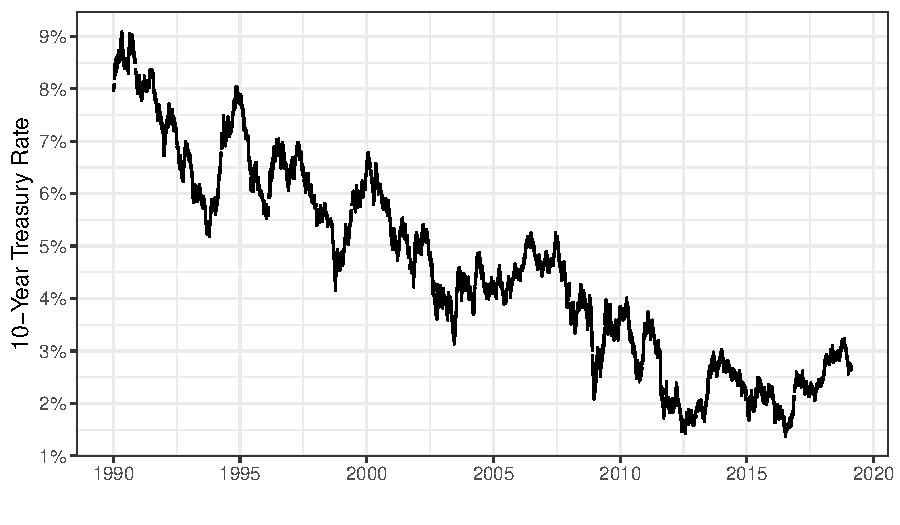
\includegraphics[width=1\linewidth]{ucla-102-fall2018_files/figure-latex/fred-DGS10-1} 

}

\caption{\textsc{10-Year Treasury Rate (Source: FRED).}}\label{fig:fred-DGS10}
\end{figure}

\begin{enumerate}
\def\labelenumi{\arabic{enumi}.}
\setcounter{enumi}{1}
\tightlist
\item
  Or, one can measure the real interest rate by using the rate on
  \textbf{Treasury Inflation Protected Securities (TIPS)}. Figure
  \ref{fig:fred-DFII10} from FRED (the Federal Reserve Economic Data)
  shows that the real interest rate has recently been around 1\% per
  year.
\end{enumerate}




\begin{figure}

{\centering 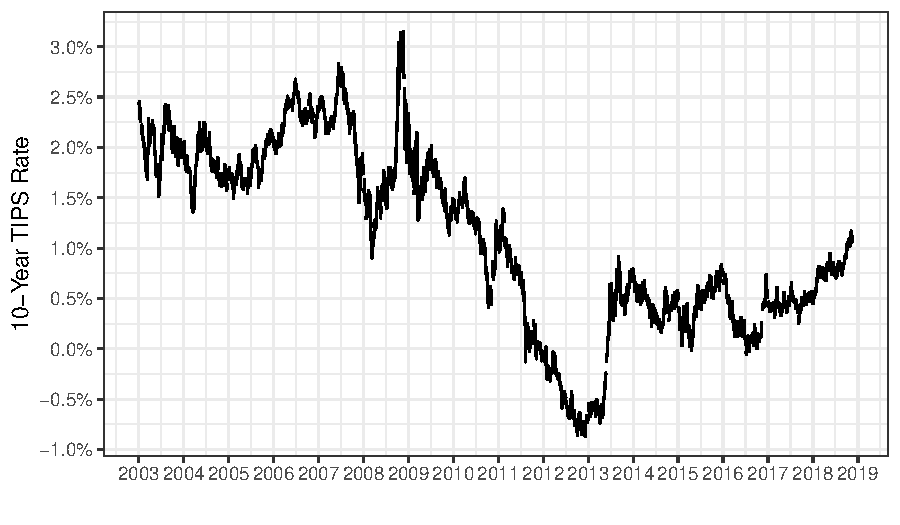
\includegraphics[width=1\linewidth]{ucla-102-fall2018_files/figure-latex/fred-DFII10-1} 

}

\caption{\textsc{10-Year Treasury Inflation Protected
Securities Rate (Source: FRED).}}\label{fig:fred-DFII10}
\end{figure}

On the other hand, real GDP growth seems to be hovering around
\(g_Y \approx 2.5\%\). Real GDP per capita growth is variable, but it is
usually estimated to be \textbf{around 1.5\%}:
\(g_{Y/L} \approx 1.5\%\). It varies over time, however: it was around
3.0\% per year on average in the 1960s, 2.1\% in the 1970s, 2.4\% in the
1980s, 2.2\% in the 1990s, 0.7\% in the 2000s, and 0.9\% from 2010 to
2017. On the other hand, the growth rate of population is \textbf{around
1\%}: \(g_{L} \approx 1.5\%\). Therefore: \[
\begin{aligned}
g_Y &= g_{Y/L} + g_L\\
&\approx 1.5\% + 1\% \\
g_Y &\approx 2.5\%.
\end{aligned}
\] Therefore, the ratio of government debt to GDP does not appear to be
on an unsustainable path so far.

A final way to see that U.S. debt is not yet on an unsustainable path is
to note that the ratio of interest payments to GDP is not particularly
high historically, which is shown on Figure \ref{fig:fred-FYOIGDA188S}.
This implies that if the primary deficit was reduced to zero, the debt
to GDP ratio would not be on an explosive trajectory.




\begin{figure}

{\centering 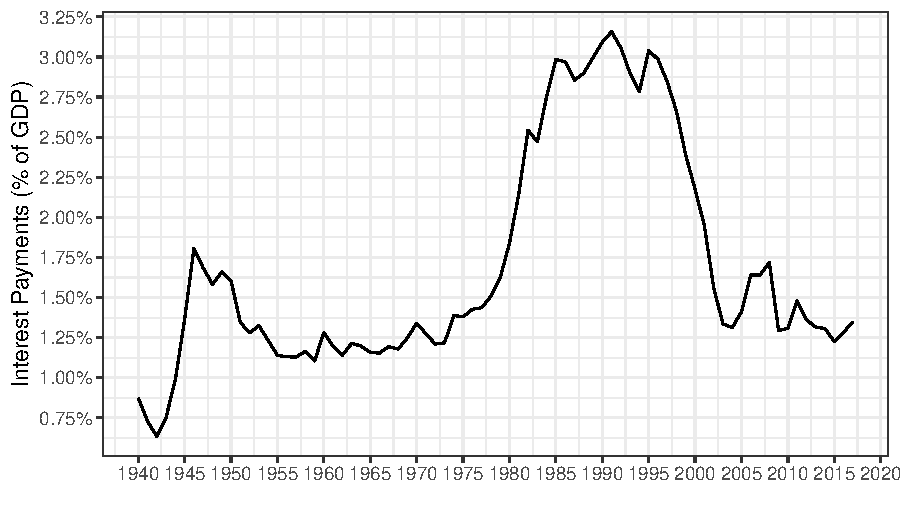
\includegraphics[width=1\linewidth]{ucla-102-fall2018_files/figure-latex/fred-FYOIGDA188S-1} 

}

\caption{\textsc{Interest Payments on Government Debt as
\% of GDP (Source: FRED).}}\label{fig:fred-FYOIGDA188S}
\end{figure}

\section{Public Debt in the Overlapping Generations
Model}\label{public-debt-in-the-overlapping-generations-model}

In this section, I illustrate using the overlapping-generations model of
\protect\hyperlink{olg}{lecture 4} that public debt does not necessarily
need to be repaid eventually, so that government debt is not necessarily
a burden on future generations - an argument which we nonetheless often
hear in the public debate. However, one precondition for this is
naturally that the debt to GDP has to be stable. In other words, we need
that \(r^{*} \leq g_Y\). In the overlapping-generations model of
\protect\hyperlink{olg}{lecture 4}, we had \(g_Y = 0\), since there was
no long-run growth. So we want \(r^{*} \leq 0\). In order to have a role
for public debt, we will look at the model that we studied in
\href{pset3.html}{Problem Set 3} called ``Another Overlapping
Generations Model'' - the solution to this problem set was available
\href{pset3-sol.html}{here}.

\subsection{Overlapping Generations
Model}\label{overlapping-generations-model}

Let us look at a simplified version of the overlapping generations model
we looked at in \protect\hyperlink{olg}{Lecture 4}. For this model, we
shall assume that people only care about old age consumption, and that
they work only when young, receiving wage \(w_{t}\). It does not really
matter what the form of their utility function is with respect to old
age consumption, because they will save everything anyway:
\[U=u(c_{t+1}^{o}).\] Denoting by \(r_t\) the (net) real interest rate,
their intertemporal budget constraint is then given by:
\[c_{t}^{y}+\frac{c_{t+1}^{o}}{1+r_t}=w_{t}.\] In this very simple
environment, and because consumption in young age will always optimally
be set to zero (\(c_{t}^{y}=0\)), this implies:
\[c_{t+1}^{o}=(1+r_t)w_{t}.\] Similarly to the previous time, we assume
that the labor force is fixed to unity (\(L_{t}=\bar{L}=1\)). The
production function is Cobb-Douglas:
\[Y_{t}=K_{t}^{\alpha}L_{t}^{1-\alpha}.\] Together with the previous
assumption of constant labor \(L_{t}=1\), this implies that:
\[Y_{t}=K_{t}^{\alpha}.\] From firms' optimality conditions, the wage is
just the marginal product of labor:
\[w_{t}=\frac{\partial Y_{t}}{\partial L_{t}}=(1-\alpha)K_{t}^{\alpha}L_{t}^{-\alpha}=(1-\alpha)K_{t}^{\alpha}.\]
Similarly as previously, we also get through firms' optimization on the
amount of capital that:
\[r_t+\delta=\frac{\partial Y_{t}}{\partial K_{t}}=\alpha K_{t}^{\alpha-1}.\]
Finally, for simplicity, we shall sometimes assume that the depreciation
rate is equal to \(\delta=1=100\%\). In other words, capital fully
depreciates each period - this is reasonable if you take one unit of
time to represent one generation, or about 30 years - remember that the
depreciation rate for one year was ranging from 5\% to 10\%.

\subsection{Without Government Debt}\label{without-government-debt}

Let us first remind ourselves what happens in the absence of government
debt in this model, as in \protect\hyperlink{olg}{lecture 4}. In the
absence of a government, we get even simpler expressions than the
previous time. The law of motion for capital is given as follows:
\[\Delta K_{t+1}=w_{t}-\delta K_{t}.\] Since \(w_t\) is a fraction
\(1-\alpha\) of output, this law of motion corresponds to the Solow
growth model with \(s = 1-\alpha\). The law of motion for capital is:
\[K_{t+1}=(1-\alpha) K_{t}^{\alpha}+ (1-\delta)K_t.\] This is a
difference equation for sequence \(K_{t}\) which converges to a steady
state value for the capital stock \(K^{*}\) such that: \[
\begin{aligned}
& \delta K^{*} = (1-\alpha)(K^*)^{\alpha}\\
& \quad \Rightarrow \quad K^{*}=\frac{(1-\alpha)^{\frac{1}{1-\alpha}}}{\delta^{\frac{1}{1-\alpha}}}.
\end{aligned}
\] The steady state value for the interest rate \(r^{*}\) is then such
that: \[
\begin{aligned}
r^{*}+\delta&=\alpha(K^{*})^{\alpha-1}\\
&= \alpha \left[\left(\frac{1-\alpha}{\delta}\right)^{\frac{1}{1-\alpha}}\right]^{\alpha-1}\\
r^{*}+\delta &=\frac{\delta \alpha}{1-\alpha}
\end{aligned}
\] Therefore, the steady-state value of the interest rate \(r^{*}\):
\[r^{*} = \frac{2\alpha-1}{1-\alpha}\delta.\] which, note, is negative
for \(\alpha < 1/2\). The steady state value for output \(Y^{*}\) is
then: \[
\begin{aligned}
Y^{*}&=\left(K^{*}\right)^{\alpha}\\
Y^{*}&=\frac{(1-\alpha)^{\frac{\alpha}{1-\alpha}}}{\delta^{\frac{\alpha}{1-\alpha}}}.
\end{aligned}
\] The value for the wage \(w^{*}\) is: \[
\begin{aligned}
w^{*}&=(1-\alpha)\left(K^{*}\right)^{\alpha}\\
&=(1-\alpha) \left(\frac{1-\alpha}{\delta}\right)^{\frac{\alpha}{1-\alpha}}\\
w^{*} &= \frac{\left(1-\alpha\right)^{\frac{1}{1-\alpha}}}{\delta^{\frac{\alpha}{1-\alpha}}}
\end{aligned}
\] Steady-state consumption of the old \((c^{o})^{*}\) is thus given by:
\[
\begin{aligned}
(c^{o})^{*}&=(1+r^*)w^{*}\\
(c^{o})^{*}&=\left(1+ \frac{2\alpha-1}{1-\alpha}\delta\right)\left(1-\alpha\right)^{\frac{1}{1-\alpha}}
\end{aligned}
\] \textbf{Full depreciation (\(\delta = 1\)).} Since one period here is
one generation, a useful assumption is that capital fully depreciates in
one period, so that \(\delta = 1\). Then, the previous expressions are
considerably more simple to work with: \[
\begin{aligned}
K^{*}&=\frac{(1-\alpha)^{\frac{1}{1-\alpha}}}{\delta^{\frac{1}{1-\alpha}}}=(1-\alpha)^{\frac{1}{1-\alpha}}\\
r^{*}&=\frac{2\alpha-1}{1-\alpha}\delta = \frac{2\alpha-1}{1-\alpha}\\
Y^{*}&=\frac{(1-\alpha)^{\frac{\alpha}{1-\alpha}}}{\delta^{\frac{\alpha}{1-\alpha}}} = (1-\alpha)^{\frac{\alpha}{1-\alpha}}\\
w^{*} &= \frac{\left(1-\alpha\right)^{\frac{1}{1-\alpha}}}{\delta^{\frac{\alpha}{1-\alpha}}} = (1-\alpha)^{\frac{1}{1-\alpha}}\\
(c^{o})^{*}&=\left(1+ \frac{2\alpha-1}{1-\alpha}\delta\right)\left(1-\alpha\right)^{\frac{1}{1-\alpha}}\\
&=\frac{\alpha}{1-\alpha}\left(1-\alpha\right)^{\frac{1}{1-\alpha}}\\
(c^{o})^{*}&= \alpha\left(1-\alpha\right)^{\frac{\alpha}{1-\alpha}}
\end{aligned}
\]

\textbf{Numerical Application.} With \(\delta = 1\) and
\(\alpha = 1/3\): \[
\begin{aligned}
K^{*}&=(1-\alpha)^{\frac{1}{1-\alpha}}=\left(\frac{2}{3}\right)^{3/2}=\frac{2\sqrt{2}}{3\sqrt{3}}\\
r^{*}&=\frac{2\alpha-1}{1-\alpha}=\frac{-1/3}{2/3}=-\frac{1}{2}=-50\%\\
Y^{*}&=(1-\alpha)^{\frac{\alpha}{1-\alpha}} = \left(\frac{2}{3}\right)^{1/2}=\frac{\sqrt{2}}{\sqrt{3}}\\
w^{*}&=\left(1-\alpha\right)^{\frac{1}{1-\alpha}} =\frac{2\sqrt{2}}{3\sqrt{3}}\\
(c^{o})^{*}&=\alpha\left(1-\alpha\right)^{\frac{\alpha}{1-\alpha}}=\frac{1}{3} \left(\frac{2}{3}\right)^{1/2}=\frac{\sqrt{2}}{3\sqrt{3}}
\end{aligned}
\]

\subsection{With Government Debt}\label{with-government-debt}

As we saw in \protect\hyperlink{solow}{lecture 2}, and then again in
\protect\hyperlink{olg}{lecture 4}, because \(r^{*}<0\) we have that the
quantity of capital is higher than the Golden Rule level of the capital
stock, which is such that \(r^{*}_g=0\). Why, again, is the Golden rule
interest rate equal to 0 when there is no growth ? One quick way to
understand it is to write that in the steady-state, the consumption of
the old \((c^{o})^{*}\) is supposed to be maximized (since the old are
the only ones consuming). However, we also know that in the
steady-state, total production \(F(K^{*}, 1) = (K^{*})^{\alpha}\) is
used for two things: consuming (for the old) and repairing the capital
stock (saving equals investment equals depreciation, as in the Solow
growth model), so that:
\[(c^{o})^{*} + \delta K^{*} = (K^{*})^{\alpha} \quad \Rightarrow \quad (c^{o})^{*} = (K^{*})^{\alpha} -\delta K^{*} \]
Therefore, the Golden rule capital stock \(K^{*}_g\), which maximizes
\((c^{o})^{*}\) solves:
\[\max_{K^{*}}\quad (K^{*})^{\alpha}-\delta K^{*},\] which implies that:
\[\alpha (K^{*}_g)^{\alpha-1}=\delta.\] Moreover, we know that the
marginal product of capital
\(\partial F(K^{*}, 1)/\partial K^{*} = \alpha (K^{*}_g)^{\alpha-1}\) is
also equal to \(r^{*}_g+\delta\), the gross return, from the firms'
problem, which gives the following optimality condition:
\[\alpha (K^{*}_g)^{\alpha-1}=r^{*}_g+\delta.\] Using these two last
equalities allows to conclude that in this situation with no growth, the
Golden rule interest rate is equal to zero since
\(r^{*}_g+\delta = \alpha (K^{*}_g)^{\alpha-1} =\delta\): \[r^{*}_g=0.\]
However, we saw in the previous section that the \emph{equilibrium}
interest rate \(r^{*}\) was negative, equal to -50\%. Therefore, the
capital stock is too high here. As we saw in lectures
\protect\hyperlink{solow}{2} and \protect\hyperlink{olg}{4}, one way to
solve this problem would be to force everyone to save less, in order to
decrease private saving; however this might be thought of as a little
bit too intrusive. Another way to solve this problem is to use public
debt (decrease public saving, to reduce total saving) in order to solve
this problem of excess saving and excess investment.

In order to better understand which level of public debt is warranted,
we look at the level of capital such that \(r^{*}_g=0\) - which again,
is the golden rule interest rate, since the rate of growth of output is
\(g_Y=0\). Thus, the corresponding Golden Rule level of the capital
stock \(K^{*}_g\) is such that:
\[r^{*}_g+\delta=\alpha (K^{*}_g)^{\alpha-1} \quad \Rightarrow_{r^{*}_g=0} \quad \delta=\alpha (K^{*}_g)^{\alpha-1}\]
Therefore: \[
\begin{aligned}
K^{*}_g=\frac{\alpha^{\frac{1}{1-\alpha}}}{\delta^{\frac{1}{1-\alpha}}}.
\end{aligned}
\] The Golden rule steady-state value for output \(Y^{*}_g\) would be
then: \[
\begin{aligned}
Y^{*}_g&=\left(K^{*}_g\right)^{\alpha}\\
Y^{*}_g&=\frac{\alpha^{\frac{\alpha}{1-\alpha}}}{\delta^{\frac{\alpha}{1-\alpha}}}.
\end{aligned}
\] The value for the steady-state wage \(w^{*}_g\) is then: \[
\begin{aligned}
w^{*}_g&=(1-\alpha)\left(K^{*}\right)^{\alpha}\\
w^{*}_g&=(1-\alpha) \frac{\alpha^{\frac{\alpha}{1-\alpha}}}{\delta^{\frac{\alpha}{1-\alpha}}}
\end{aligned}
\] Steady-state consumption of the old \((c^{o})^{*}_g\) is thus given
by: \[
\begin{aligned}
(c^{o})^{*}_g&=(1+r^*)w^{*}_g\\
(c^{o})^{*}_g&=(1-\alpha) \frac{\alpha^{\frac{\alpha}{1-\alpha}}}{\delta^{\frac{\alpha}{1-\alpha}}}
\end{aligned}
\] If \(\delta = 1\), then:
\[(c^{o})^{*}_g=(1-\alpha) \alpha^{\frac{\alpha}{1-\alpha}}\] The
question is how to we achieve this quantity of capital \(K^{*}_g\)? The
answer is that some public debt needs to be taken on by the government.
Again, saving is equal to the wage \(w^{*}_g\), and to the purchase of
total assets, which includes both public debt whose quantity is given by
\(B^{*}_g\), and the capital stock whose quantity is \(K^{*}_g\).
Therefore, we may compute the level of the public debt which allows to
reach this Golden-Rule level of capital accumulation:
\[B^{*}_g+K^{*}_g=w^{*}_g\quad\Rightarrow\quad B^{*}_g=w^{*}_g-K^{*}_g.\]
Substituting: \[
\begin{aligned}
B^{*}_g&=w^{*}_g-K^{*}_g\\
&=(1-\alpha) \frac{\alpha^{\frac{\alpha}{1-\alpha}}}{\delta^{\frac{\alpha}{1-\alpha}}}-\frac{\alpha^{\frac{1}{1-\alpha}}}{\delta^{\frac{1}{1-\alpha}}}\\
B^{*}_g&=\frac{\alpha^{\frac{\alpha}{1-\alpha}}}{\delta^{\frac{\alpha}{1-\alpha}}}\left(1-\alpha-\frac{\alpha}{\delta}\right).
\end{aligned}
\] Note that with \(\delta = 1\), then this level of public debt is
strictly positive when \(\alpha <1/2\).

\textbf{Numerical Application.} With \(\alpha = 1/3\) and
\(\delta = 1\): \[
\begin{aligned}
K^{*}_g&=\frac{\alpha^{\frac{1}{1-\alpha}}}{\delta^{\frac{1}{1-\alpha}}}=\left(\frac{1}{3}\right)^{3/2} = \frac{1}{3\sqrt{3}}\\
r_g^{*}&=0\\
Y_g^{*}&=\frac{\alpha^{\frac{\alpha}{1-\alpha}}}{\delta^{\frac{\alpha}{1-\alpha}}} = \left(\frac{1}{3}\right)^{1/2}=\frac{1}{\sqrt{3}}\\
w^{*}_g&=(1-\alpha) \frac{\alpha^{\frac{\alpha}{1-\alpha}}}{\delta^{\frac{\alpha}{1-\alpha}}}= \frac{2}{3}\sqrt{\frac{1}{3}} = \frac{2}{3\sqrt{3}}\\
(c^{o})^{*}_g&=(1+r^*_g)w^{*}_g=w^{*}_g = \frac{2}{3\sqrt{3}}
\end{aligned}
\] Note that the steady-state consumption of the old \((c^{o})^{*}_g\)
is greater than the level of consumption achieved by the old without
government debt since \(2>\sqrt{2}\). But what is amazing is that the
level of capital in this case is actually lower than the level of
capital in the previous section. The government can force the economy
into this level of capital accumulation by taking on debt. The level of
debt \(B^{*}_g\) that corresponds to that level of capital accumulation
is given by: \[
\begin{aligned}
B^{*}_g&=w^{*}_g-K^{*}_g\\
&=\frac{2}{3\sqrt{3}}-\frac{1}{3\sqrt{3}}\\
B^{*}_g&=\frac{1}{3\sqrt{3}}.
\end{aligned}
\]\\
The government can reach that level of debt by giving a transfer to the
first generation of old, like the war veterans, who will then consume in
the first period \(t=0\) an amount equal to:
\[c_{0}^{o}=\frac{\sqrt{2}}{3\sqrt{3}}+\frac{1}{3\sqrt{3}}=\frac{1+\sqrt{2}}{3\sqrt{3}}.\]
All future generations thus consume more. With a lot of capital, there
is such a thing as a free lunch! Public debt is a Ponzi scheme, but a
beneficial one. Public debt allows to increase consumption for everyone,
and it can be rolled over every period (note that the debt to GDP ratio
stays constant, as GDP growth is zero in the long run, just as the long
run interest rate is zero). This is true more generally even in the
neoclassical model, provided that there is \textbf{dynamic inefficiency}
(\(r^*<g_Y\)) to begin with.

\section{The Treasury View, and Say's
Law}\label{the-treasury-view-and-says-law}

The most controversial and also most important questions in
macroeconomics revolve around the issue of the so-called
\textbf{Treasury View}, and \textbf{Say's law}. These are probably the
most difficult, controversial, but also the most important questions for
macroeconomics.

\subsection{Treasury View: The Effects of Deficit Spending on
Investment}\label{treasury-view-the-effects-of-deficit-spending-on-investment}

The \emph{Treasury View} asserts that more government spending, either
in the form of government purchases or of tax reductions, and therefore
lower saving, necessarily leads to \emph{crowd out} (reduce) an equal
amount of investment spending. Conversely more saving, either by the
government or by households, leads to more investment. The logic of this
argument is rather straightforward: if there exists a finite amount of
resources in the economy - in other words, output is supply-determined -
then whatever is being saved goes to increase investment. Output is
simply the sum of consumption, investment, and government spending, so
that ``necessarily'' increasing government spending leads to crowd out
either of every component: \[
\begin{aligned}
&Y = C+I+G\\
\quad &  \Rightarrow \quad \left(Y- C-T\right)=I+\left(G-T\right) \\
\quad &  \Rightarrow \quad \left(Y- C-T\right) + \left(T-G\right)=I
\end{aligned}
\] Therefore investment \(I\) equals total saving, private saving
\(S=Y-C-T\) plus public saving \(T-G\):
\[\boxed{I = \underbrace{\left(Y-C-T\right)}_{\text{Private Saving}} + \underbrace{(T-G)}_{\text{Public Saving}}}\]
The reason why this view is called the \textbf{Treasury View} is that it
was advanced in the 1930s, during the Great Depression, by the staff of
the British Chancellor of the Exchequer, Winston Churchill. When
defending his 1929 budget, Winston Churchill explained:

\begin{quote}
The orthodox Treasury view\ldots{} is that when the Government borrows
in the money market it becomes a new competitor with industry and
engrosses to itself resources which would otherwise have been employed
by private enterprise, and in the process raises the rent of money to
all who have need of it.
\end{quote}

What we have seen so far leads us to take a very constrasted perspective
on the Treasury View:

\begin{itemize}
\item
  In the \textbf{Keynesian model} of lectures
  \protect\hyperlink{cons-function}{7},
  \protect\hyperlink{paradox-thrift}{8}, and
  \protect\hyperlink{redistributive}{9}, investment is not crowded out
  by public debt - in the simplest model of the goods market, investment
  is in fact fixed. In the accelerator model, \(I=b_0 + b_1 Y\) so that
  investment depends only on sales, not on saving. According to this
  model, what the Treasury View misses is that output is not determined
  by supply, but it is instead determined by demand. Therefore, one
  cannot reason as if GDP was fixed: GDP is precisely what adjusts when
  saving is reduced, to maintain the equality between investment and
  total saving.
\item
  In the \textbf{neoclassical model} of lectures
  \protect\hyperlink{solow}{2} and \protect\hyperlink{olg}{4} in
  contrast, investment is determined by total saving, and it moves
  flexibly in response to saving. According to this view, investment is
  indeed crowded out by public deficits. Note however that this does not
  mean that in the neoclassical model, government deficits are always
  bad. As we just saw, public deficits may be a good thing if the
  economy has too much capital to begin with.
\end{itemize}

This issue of the Treasury view was discussed a lot during the U.S. 2008
financial crisis, when policymakers were turning to economists for
advice on the appropriate policy response. You can see some discussion
of this issue in ``Readings - To go further''. While Chicago economists
were articulating the Treasury view in various different flavors,
Keynesian economists were rejecting this notion very strongly - most
notably Paul Krugman. Of course, whether the Treasury View is correct or
not is ultimately an empirical question. We will present some empirical
evidence on this issue during lecture 13.

\subsection{Say's law: supply creates its own
demand}\label{says-law-supply-creates-its-own-demand}

Say's law, named after Jean-Baptiste Say (1767 - 1832), has been
summarized by J.M. Keynes as a statement that ``supply creates its own
demand''. Jean-Baptiste Say's reasoning was straightforward:

\begin{quote}
It is worthwhile to remark that a product is no sooner created than it,
from that instant, affords a market for other products to the full
extent of its own value. When the producer has put the finishing hand to
his product, he is most anxious to sell it immediately, lest its value
should diminish in his hands. Nor is he less anxious to dispose of the
money he may get for it; for the value of money is also perishable. But
the only way of getting rid of money is in the purchase of some product
or other. Thus the mere circumstance of creation of one product
immediately opens a vent for other products.
\end{quote}

Thus, in Say's opinion, supply created its own demand, and there could
never be any aggregate demand shortages. In a
\href{https://www.economist.com/economics-brief/2017/08/10/says-law-supply-creates-its-own-demand}{briefing}
on Say's law, \emph{The Economist} magazine writes:

\begin{quote}
In Say's time, as nowadays, the world economy combined strong
technological progress with fitful demand, spurts of innovation with
bouts of austerity. (\ldots{}) On the other hand, global demand was
damaged by failed ventures in South America and debilitated by the
eventual downfall of Napoleon. In Britain government spending was cut by
40\% after the Battle of Waterloo in 1815. Some 300,000 discharged
soldiers and sailors were forced to seek alternative employment. The
result was a tide of overcapacity, what Say's contemporaries called a
``general glut''. Britain was accused of inundating foreign markets,
from Italy to Brazil, much as China is blamed for dumping products
today. In 1818 a visitor to America found ``not a city, nor a town, in
which the quantity of goods offered for sale is not infinitely greater
than the means of the buyers''. It was this ``general overstock of all
the markets of the universe'' that came to preoccupy Say and his
critics. In trying to explain it, Say at first denied that a ``general''
glut could exist. Some goods can be oversupplied, he conceded. But goods
in general cannot. His reasoning became known as Say's law: ``it is
production which opens a demand for products'', or, in a later, snappier
formulation: supply creates its own demand.
\end{quote}

Once again, we may contrast two very different perspectives on the Say's
law:

\begin{itemize}
\item
  In the \textbf{Keynesian model} of lectures
  \protect\hyperlink{cons-function}{7},
  \protect\hyperlink{paradox-thrift}{8}, and
  \protect\hyperlink{redistributive}{9}, supply does not create its own
  demand, as some resources (labor or capital) are idle. This allows
  government spending or tax cuts to have an effect on GDP, by utilizing
  some of these resources. The reason is that in this model, the desire
  to save does not necessarily translate into more investment, since
  investment is fixed or given by the overall level of GDP, which is
  depressed by more saving. This was the paradox of thrift of
  \href{lecture8.html}{lecture 8}: instead of increasing investment, a
  higher desire to save actually reduces output, which ends up
  depressing saving.
\item
  In the \textbf{neoclassical model} of lectures
  \protect\hyperlink{solow}{2} and \protect\hyperlink{olg}{4} in
  contrast, investment is determined by total saving, and it moves
  flexibly in response to saving. According to this view, there can
  indeed never be a general glut: consumption increases aggregate
  demand, but saving increases it too, by stimulating more investment.
  True, there might be ``too much capital'', when the capital stock is
  higher than the Golden rule level, but this is not a ``general glut''.
  Thus, supply can be thought of as indeed ``creating its own demand''.
\end{itemize}

How you stand on those two issues (the Treasury View and Say's law)
determines whether you are more a neoclassical or a Keynesian economist.
As we have seen however, Keynesians and neoclassicals agree on one
thing: consumption is the sole purpose of all production, and there
exists such a thing as ``too much capital'', when \(r^{*}<g_Y\). Whether
that is the situation we are in, even after Donald Trump's massive tax
cuts, is still a controversial question.

\section*{Readings - To go further}\label{readings---to-go-further-7}
\addcontentsline{toc}{section}{Readings - To go further}

\href{https://doi.org/10.2307/1882763}{Uriel H. Crocker and S. M.
Macvane, ``General Overproduction,'' The Quarterly Journal of Economics
1, no. 3 (1887): 362--66.}

\href{https://search.proquest.com/docview/399114897/CBD1D9A468D04A85PQ/2?accountid=14512}{Robert
J. Barro, Government Spending Is No Free Lunch, \emph{Wall Street
Journal}, January 22, 2009.}

\href{https://search.proquest.com/docview/1930920374/1A771BC8177A4FB7PQ/1?accountid=14512}{Paul
Krugman, A Dark Age of Macroeconomics (wonkish), \emph{New York Times},
Jan 27, 2009}

\href{https://krugman.blogs.nytimes.com/2015/06/03/multipliers-and-reality/}{Paul
Krugman, Multipliers and Reality, New York Times Blog Post, June 3,
2015.}

\href{https://search.proquest.com/docview/1768757479/E1052F8FA6974859PQ/1?accountid=14512}{In
Japan, the Government Gets Paid to Borrow Money, \emph{Wall Street
Journal}, March 1, 2016.}

(Gated)
\href{https://www.economist.com/economics-brief/2017/08/10/says-law-supply-creates-its-own-demand}{Say's
Law: Supply Creates its Own Demand. \emph{The Economist}, August 10,
2017.}

(Gated)
\href{https://www.economist.com/economics-brief/2017/08/31/kicking-the-can-down-an-endless-road}{Overlapping
Generations: Kicking the road down an endless road. \emph{The
Economist}, August 31, 2017.}

(Gated)
\href{https://www.economist.com/finance-and-economics/2018/08/09/why-is-macroeconomics-so-hard-to-teach}{Why
is macroeconomics so hard to teach? \emph{The Economist}, August 9,
2018.}

\href{https://search.proquest.com/docview/2131663609/B6DB7A44958C4606PQ/1?accountid=14512}{``U.S.
on a course to spend more on debt than defense'', \emph{Wall Street
Journal}, November 11, 2018.}

\appendix


\hypertarget{pset1}{\chapter{Problem Set 1}\label{pset1}}

\section{Geometric Sums}\label{geometric-sums}

\begin{enumerate}
\def\labelenumi{\arabic{enumi}.}
\item
  Calculate the following geometric sum, when \(x \neq 1\), as a
  function of \(x^{n+1}\) in particular:
  \[\sum_{i=0}^n x^i = 1+x+x^2+...+x^n\]
\item
  State a condition on \(x\) such that the infinite geometric sum (when
  \(n \to \infty\)) has a finite value.
\item
  Assuming that this geometric sum is finite, calculate:
  \[\sum_{i=0}^{\infty} x^i = 1+x+x^2+...+x^n+...\]
\item
  More generally, for \(m\) a positive integer, calculate:
  \[\sum_{i=m}^n x^i = x^m+x^{m+1}+...+x^n\]
\item
  What is the present discounted value of an infinite stream of incomes,
  which grows at rate \(g=2\) \%, starts at \(y_0=90000\), if the
  interest rate is \(i=3\) \%?
\end{enumerate}

\section{Taylor Approximations}\label{taylor-approximations}

\begin{enumerate}
\def\labelenumi{\arabic{enumi}.}
\item
  If \(x\) is small, show that: \[(1+x)^n \approx 1+nx.\]
\item
  If \(x\) and \(y\) are small, then show that:
  \[(1+x)(1+y) \approx 1+x+y.\]
\item
  If \(x\) and \(y\) are small, then show that:
  \[\frac{1+x}{1+y} \approx 1+x-y.\]
\item
  Your savings account offers a nominal interest rate of 1\%. Meanwhile,
  annual inflation is 1.5\%. What is an exact value for the real
  interest rate, defined as the rate of increase in your purchasing
  power if you leave your money in the bank? What is an approximate
  value for this real interest rate, using one of the previous formulas?
\end{enumerate}

\section{Growth Rates}\label{growth-rates}

\begin{enumerate}
\def\labelenumi{\arabic{enumi}.}
\item
  If \(y_t\) grows at a constant rate \(g\) during a given period, then
  show that the growth \(G\) of \(y_t\) after \(T\) periods is:
  \[G = \frac{y_T}{y_0}-1=(1+g)^T-1.\]
\item
  Conversely, if the growth rate of \(y_t\) after \(T\) periods is
  \(G\), then show that the average growth rate of \(y_t\) per period
  is: \[g = \frac{y_{t+1}}{y_{t}}-1=(1+G)^{1/T}-1.\]
\item
  If your annual return on your savings rate is 1\%, what is your daily
  return (assuming a year is 365 days)? How much do you then give up
  each day by leaving \$100K on a zero interest checking account?
\end{enumerate}

\hypertarget{pset2}{\chapter{Problem Set 2}\label{pset2}}

\section{\texorpdfstring{Solow Growth Model if \(\alpha = 1/2\) and
\(A=1/2\)}{Solow Growth Model if \textbackslash{}alpha = 1/2 and A=1/2}}\label{solow-growth-model-if-alpha-12-and-a12}

Suppose that the production function is such that \(A=1/2\) (often, we
assume that \(A=1\)) and \(\alpha=1/2\):
\[Y=\frac{1}{2}\sqrt{K}\sqrt{L}\]

\begin{enumerate}
\def\labelenumi{\arabic{enumi}.}
\item
  Derive the steady-state levels of output per worker and capital per
  worker in terms of the saving rate, \(s\), and the depreciation rate,
  \(\delta\).
\item
  Derive the equation for steady-state output per worker and
  steady-state consumption per worker in terms of \(s\) and \(\delta\).
\item
  Suppose that \(\delta=0.05\). With your favorite spreadsheet software,
  compute steady-state output per worker and steady-state consumption
  per worker for \(s=0\); \(s=0.1\); \(s=0.2\); \(s=1\). Explain the
  intuition behind your results.
\item
  Use your favorite spreadsheet software to graph the steady-state level
  of output per worker and the steady-state level of consumption per
  worker as a function of the saving rate (i.e., measure the saving rate
  on the horizontal axis of your graph and the corresponding values of
  output per worker and consumption per worker on the vertical axis).
\item
  Does the graph show that there is a value of \(s\) that maximizes
  output per worker? Does the graph show that there is a value of \(s\)
  that maximizes consumption per worker? If so, what is this value?
\end{enumerate}

\section{\texorpdfstring{Solow Growth Model if
\(\alpha = 1/3\)}{Solow Growth Model if \textbackslash{}alpha = 1/3}}\label{solow-growth-model-if-alpha-13}

Suppose that the economy's production function is given by
\[Y=K^{\alpha}L^{1-\alpha}\] and assume that \(\alpha=1/3\).

\begin{enumerate}
\def\labelenumi{\arabic{enumi}.}
\item
  Is this production function characterized by constant returns to
  scale? Explain.
\item
  Are there decreasing returns to capital?
\item
  Are there decreasing returns to labor?
\item
  Transform the production function into a relation between output per
  worker and capital per worker.
\item
  For a given saving rate, \(s\), and depreciation rate, \(\delta\),
  give an expression for capital per worker in the steady state.
\item
  Give an expression for output per worker in the steady state.
\item
  Solve for the steady-state level of output per worker when \(s=0.32\)
  and \(\delta=0.08\).
\item
  Suppose that the depreciation rate remains constant at
  \(\delta=0.08\), while the saving rate is reduced by half, to
  \(s=0.16\). What is the new steady-state output per worker?
\end{enumerate}

\section{An increase in the depreciation
rate}\label{an-increase-in-the-depreciation-rate}

Continuing with the logic from the previous problem, suppose that the
economy's production function is given by \[Y=K^{\alpha}L^{1-\alpha}\]
with \(\alpha=1/3\) and that both the saving rate, \(s\), and the
depreciation rate, \(\delta\) are equal to \(0.10\).

\begin{enumerate}
\def\labelenumi{\arabic{enumi}.}
\item
  What is the steady-state level of capital per worker?
\item
  What is the steady-state level of output per worker? Suppose that the
  economy is in steady state and that, in period \(t\), the depreciation
  rate increases permanently from \(0.10\) to \(0.20\).
\item
  What will be the new steady-state levels of capital per worker and
  output per worker?
\item
  Compute the path of capital per worker and output per worker over the
  first three periods after the change in the depreciation rate.
\end{enumerate}

\section{Deficits and the capital
stock}\label{deficits-and-the-capital-stock}

Suppose that the production function is given by: \[Y=\sqrt{K}\sqrt{L}\]

\begin{enumerate}
\def\labelenumi{\arabic{enumi}.}
\item
  Show that the steady-state capital stock per worker and output per
  worker are given by:
  \[\frac{K^{*}}{L}=\left(\frac{s}{\delta}\right)^{2} \quad \text{and} \quad \frac{Y^{*}}{L}=\frac{s}{\delta}.\]
\item
  Suppose that the saving rate, \(s\), is initially 15 \% per year, and
  the depreciation rate, \(\delta\), is 7.5 \%. What is the steady-state
  capital stock per worker? What is steady-state output per worker?
\item
  Suppose that there is a government deficit of 5\% of GDP and that the
  government eliminates this deficit. Assume that private saving is
  unchanged so that total saving increases to 20\%. What is the new
  steady-state capital stock per worker? What is the new steady-state
  output per worker? How does this compare to your answer to part 2?
\end{enumerate}

\section{U.S. saving and government
deficits}\label{u.s.-saving-and-government-deficits}

This question continues the logic of the previous question, to explore
the implications of the U.S. government budget deficit for the long-run
capital stock.

\begin{enumerate}
\def\labelenumi{\arabic{enumi}.}
\item
  The World Bank reports gross domestic saving rate by country and year.
  The Web site is
  \url{http://data.worldbank.org/indicator/NY.GDS.TOTL.ZS}. Find the
  most recent number for the United States. What is the total saving
  rate in the United States as a percentage of GDP? Using the
  depreciation rate and the logic from the previous problem, what would
  be the steady-state capital stock per worker? What would be
  steady-state output per worker?
\item
  Go to the most recent Economic Report of the President (ERP) and find
  the most recent federal deficit as a percentage of GDP. In the 2015
  ERP, this is found in Table B-20. Using the reasoning from the
  previous problem, suppose that the federal budget deficit was
  eliminated and there was no change in private saving. What would be
  the effect on the long-run capital stock per worker? What would be the
  effect on long-run output per worker?
\item
  Return to the World Bank table of gross domestic saving rates. How
  does the saving rate in China compare to the saving rate in the United
  States?
\end{enumerate}

\hypertarget{pset3}{\chapter{Problem Set 3}\label{pset3}}

\section{Two-period Intertemporal
Optimization}\label{two-period-intertemporal-optimization}

Consider the model of \protect\hyperlink{two-period}{lecture 3} again.
Instead of logarithmic preferences, assume that preferences are given
by:

\[u(c) = \frac{c^{1-\sigma}-1}{1-\sigma},\]

\begin{enumerate}
\def\labelenumi{\arabic{enumi}.}
\item
  Under what condition on \(\sigma\) is this an increasing and concave
  utility function?
\item
  Show using 4 different methods that:
  \[\frac{\beta u'(c_{1})}{u'(c_{0})}=\frac{1}{1+r}\]
\item
  Using the equation in question 1, what is the ratio \(c_1/c_0\)?
\item
  Replace in the intertemporal budget constraint to find an implicit
  equation for \(c_1\). Do the same for \(c_0\).
\item
  Assume that \(\sigma = 1/2\), and \(f_0=0\), \(y_0=\$90,000\),
  \(y_1=0\), \(\beta = 1\). What are \(c_0\) and \(c_1\) if \(r=1\%\)?
  What about if \(r=2\%\)? How much does \(c_0\) change then? How much
  in percentage terms?
\item
  Same questions if \(\sigma = 1\).
\item
  Same questions if \(\sigma = 2\).
\item
  Compare the changes in \(c_0\) following an increase in the real
  interest rates in questions 5, 6, 7. Comment.
\end{enumerate}

\section{Another Overlapping Generations
model}\label{another-overlapping-generations-model}

Consider the model of \protect\hyperlink{olg}{lecture 4} again, with one
small twist: agents care only about old age consumption. In other words,
their utility functions are given by: \[U=u(c_{t+1}^{o}).\] Our goal is
to derive the law of motion for the capital stock \(K_t\), that is, a
function relating \(K_{t+1}\) to \(K_t\) and the parameters of the
model.

\begin{enumerate}
\def\labelenumi{\arabic{enumi}.}
\item
  Why can the utility function be left unspecified for computing the
  level of saving?
\item
  Derive the law of motion for capital.
\item
  What is the corresponding value of the saving rate in the Solow model?
\item
  Provide a condition on \(\alpha\) such that the capital stock is below
  the Golden Rule level.
\item
  Is that condition likely to be satisfied?
\end{enumerate}

\hypertarget{pset4}{\chapter{Problem Set 4}\label{pset4}}

\section{The Solow Growth Model with Exogenous
Growth}\label{the-solow-growth-model-with-exogenous-growth}

Consider the Solow growth model of \protect\hyperlink{solow}{Lecture 2},
with however two small changes. Assume that the production function is
given by: \[F(K_t,L_t)=A_t K_t^{\alpha} L_t^{1-\alpha},\] where
productivity \(A_t\) grows exogenously at rate \(g\) and \(A_0=1\):
\[A_t=(1+g)^t.\] Moreover, assume that the labor force also grows at a
rate \(n\) and \(L_0=1\), so that at any time \(t\): \[ L_t = (1+n)^t.\]

\begin{enumerate}
\def\labelenumi{\arabic{enumi}.}
\item
  Write the law of motion for capital \(K_t\).
\item
  Define \(k_t\) as: \[ k_t\equiv\frac{K_t}{A_t^{1/(1-\alpha)} L_t},\]
  and write a law of motion for \(k_t\). Assume that \(n\), and \(g\)
  are small in order to simplify this law of motion. \emph{Hint}: if
  \(n\) and \(g\) are small then:
  \((1+g)^{1/(1-\alpha)}(1+n) \approx 1+\frac{1}{1-\alpha}g+n.\)
\item
  Show that \(k_t\) converges to a steady-state \(k^{*}\). Compute
  \(k^{*}\).
\item
  When \(k_t\) has reached a steady-state, the economy is said to be on
  a \textbf{balanced growth path}. On this balanced growth path, what is
  the rate of growth of \(Y_t\), \(C_t\), \(K_t\), \(K_t/Y_t\),
  \(K_t/L_t\), \(w_t\), \(w_t L_t\) and \(w_t L_t/Y_t\) ? Denoting by
  \(R_t\) the marginal product of capital, what is the rate of growth of
  \(R_t\), \(R_t K_t\), and \(R_t K_t/Y_t\) ?
\item
  Compute \(y^{*}\) and \(c^{*}\) corresponding to steady-state
  \(k^{*}\) with:
  \[y_t \equiv \frac{Y_t}{A_t^{1/(1-\alpha)} L_t} \quad \text{and} \quad c_t \equiv \frac{C_t}{A_t^{1/(1-\alpha)} L_t}.\]
\item
  What is the saving rate which maximizes \(c^{*}\) ? (Golden Rule level
  of capital accumulation)
\item
  What is then the value of the marginal product of capital \(R^{*}\) ?
\end{enumerate}

\section{The Neoclassical Labor Market
Model}\label{the-neoclassical-labor-market-model}

Consider the neoclassical labor market model of
\protect\hyperlink{labor-market}{lecture 6}. Assume that preferences and
the production function are as in
\protect\hyperlink{labor-market}{lecture 6}:
\[U(c, l)=c-B\frac{l^{1+\epsilon}}{1+\epsilon}, \qquad f(l)=Al^{1-\alpha}.\]
Denote the wage by \(w\), and the price of consumption by \(p\).

\begin{enumerate}
\def\labelenumi{\arabic{enumi}.}
\item
  Derive the Labor Demand curve.
\item
  Assume that \(\alpha=1/3\) and \(A=2\). Using your favorite
  spreadsheet software, plot this demand curve in a \((l, w/p)\) plane -
  that is, putting \(l\) on the x-axis and \(w/p\) on the y-axis.
\item
  Take logs of both sides. What does the demand curve look like in a
  \((\log(l), \log(w/p))\) plane? What is the slope of the demand curve
  equal to? If \(\alpha\) is higher, is the demand curve steeper or
  flatter? What shifts the demand curve to the left or to the right?
\item
  Derive the Labor Supply curve.
\item
  Assume that \(\epsilon=5\) and \(B=2\). Using your favorite
  spreadsheet software, plot this supply curve in a \((l, w/p)\) plane -
  that is, putting \(l\) on the x-axis and \(w/p\) on the y-axis. Add
  the supply curve to the demand curve of question 2.
\item
  Take logs of both sides. What does the supply curve look like in a
  \((\log(l), \log(w/p))\) plane? What is the slope of the supply curve
  equal to? If \(\epsilon\) is higher, is the supply curve steeper or
  flatter? What shifts the supply curve to the left, or to the right?
\item
  Assume that productivity \(A\) decreases by 5\%, to \(A=1.9\). What is
  the effect on the quantity of employment, and on the real wage? If
  \(\alpha\) is higher, is that effect larger or smaller? What is the
  economic intuition?
\item
  Assume that leisure becomes relatively more attractive relative to
  working (think of Facebook, Netflix, etc.), so that \(B\) increases by
  10\% (the disutility of work increases). What is the effect on the
  quantity of employment, and on the real wage? If \(\epsilon\) is
  higher, is that effect larger or smaller? What is the economic
  intuition for this?
\end{enumerate}

\section{\texorpdfstring{The ``Keynesian'' Labor Market
Model}{The Keynesian Labor Market Model}}\label{the-keynesian-labor-market-model}

Consider the neoclassical labor market model of the previous problem.

\begin{enumerate}
\def\labelenumi{\arabic{enumi}.}
\item
  Assume that productivity \(A\) decreases by 5\%, but that real wages
  \(w/p\) are rigid. Compute the change in the quantity of employment
  following a fall in productivity.
\item
  Compare the effect with question 7 in the previous problem. Explain.
\item
  Assume that leisure becomes relatively more attractive relative to
  working, so that \(B\) increases by 10\%. Compute the change in the
  quantity of employment following a increase in leisure attractiveness.
\item
  Compare the effect with question 8 in the previous problem. Explain.
\end{enumerate}

\section{The Bathtub model}\label{the-bathtub-model}

Consider the bathtub model of \protect\hyperlink{labor-market}{lecture
6}. Assume a monthly job separation rate equal to \(s=1\)\%, and a
monthly job finding rate equal to \(f=20\)\%. Assume that the labor
force is given by \(L=159\) million.

\begin{enumerate}
\def\labelenumi{\arabic{enumi}.}
\item
  Derive the steady-state unemployment rate. How many people are
  unemployed in the steady-state? How many people lose their jobs every
  month? How many people find a job every month?
\item
  Assume that the economy starts with an unemployment rate equal to
  \(u_0=8\)\%. Using your favorite spreadsheet software, show the
  evolution of the unemployment rate over time. How long before the
  unemployment rate reaches 5\%?
\item
  If \(s=2\)\% instead, which job finding rate \(f\) gives the same
  steady-state unemployment rate?
\item
  Assuming the separation rate and the job finding rate are given from
  question 3, answer question 2 again.
\item
  Explain why an economy with more churning (that is, faster
  reallocation) - think of the US versus Europe - has a faster recovery
  in terms of unemployment after a recession. \emph{Note:} A recession
  could be coming from a temporary increase in the job separation rate,
  or a temporary decrease in the job finding rate, which then goes back
  to its original value.
\end{enumerate}

\hypertarget{pset5}{\chapter{Problem Set 5}\label{pset5}}

\section{Gregory N. Mankiw - NYT - Nov 30,
2008}\label{gregory-n.-mankiw---nyt---nov-30-2008}

This exercise is based on the following \emph{New York Times} article,
which Gregory N. Mankiw wrote a bit more than 2 months after the
bankruptcy of Lehman Brothers (to which we shall come back at the end of
the class). The \emph{New York Times} articles are gated after you have
read your monthly quota, but archives are available through UCLA on
ProQuest:

\href{https://search.proquest.com/docview/433963341/fulltext/43832006CCFE4D96PQ/1?accountid=14512}{Mankiw,
N. Gregory. What would Keynes have done? \emph{New York Times}, November
30, 2008}

\begin{enumerate}
\def\labelenumi{\arabic{enumi}.}
\item
  According to Gregory N. Mankiw, which factors contributed to hold back
  consumption? Can you interpret these factors in terms of changes in
  \(c_0\)?
\item
  Gregory N. Mankiw mentions the ``paradox of thrift''. Which model that
  we saw in the class makes most sense of his explanations?
\item
  Concerning saving, one of the arguments that Gregory N. Mankiw makes
  is more neoclassical. Which one is it?
\item
  What is Gregory N. Mankiw most concerned about though?
\end{enumerate}

\section{Procyclical Government
spending}\label{procyclical-government-spending}

Consider the basic goods market model of
\protect\hyperlink{cons-function}{Lecture 7}: consumption is linear in
disposable income, disposable income is income minus taxes, investment
is exogenous and equal to \(\bar{I}\), and taxes are exogenous as well.
However, government spending depends on the level of output. For
example, the government systematically spends more when GDP is higher
(it builds new roads, hires new teachers, etc.), and conversely when GDP
is lower (it then stops construction projects, fires teachers, etc.).
Thus, government spending is given by the following equation, with
\(g_1>0\): \[G = g_0 + g_1Y\]

\begin{enumerate}
\def\labelenumi{\arabic{enumi}.}
\item
  Solve for equilibrium output.
\item
  If \(g_1+c_1<1\), what is the value of the tax multiplier? (the tax
  multiplier is equal to the increase in output following from a \$1
  decrease in taxes) If \(g_1>0\), is the multiplier higher or lower
  than when government spending does not depend on GDP (\(g_1=0\))? What
  is the intuition for this?
\item
  Does this kind of policy appear like a good policy?
\item
  Give both a graphical as well as an algebraic justification for the
  value of the multiplier.
\item
  What happens if \(g_1+c_1>1\)? Explain using the multiplier intuition.
\end{enumerate}

\section{Accelerator and Automatic
Stabilizer}\label{accelerator-and-automatic-stabilizer}

Consider the basic goods market model of
\protect\hyperlink{cons-function}{Lecture 7}: consumption is linear in
disposable income with a Marginal Propensity to Consume equal to
\(c_1\), disposable income is income minus taxes. However, we assume an
accelerator effect of demand on investment (investment depends on
sales): \[I=b_0 + b_1 Y,\] as well as the presence of automatic
stabilizers: \[T=t_0+t_1Y.\]

\begin{enumerate}
\def\labelenumi{\arabic{enumi}.}
\item
  Solve for equilibrium output.
\item
  Find a condition on \(b_1\), \(c_1\), and \(t_1\) such that the
  multiplier stays finite.
\item
  What happens if the multiplier is infinite? Does GDP become infinite?
\item
  Give both a graphical as well as an algebraic justification for the
  value of the multiplier.
\end{enumerate}

\hypertarget{pset6}{\chapter{Problem Set 6}\label{pset6}}

\section*{Another Numerical Example}\label{another-numerical-example}
\addcontentsline{toc}{section}{Another Numerical Example}

During \protect\hyperlink{redistributive}{lecture 9}, we studied the
aggregate demand effects of tax cuts on the bottom 90\% financed by tax
increases on the top 10\%. In this problem, we study another example of
these aggregate demand effects, looking at redistribution from the top
1\% income share to the bottom 99\%. \emph{An important warning}: Again,
note that this model only has Keynesian, aggregate demand effects.
However, raising taxes on high income earners certainly has effects on
the supply side as well. Raising taxes on the top 1\% probably also has
effects on entrepreneurship, incentives to take risk and create jobs,
which are not taken into account here. (Symmetrically, changing taxes on
the bottom 99\% also may have effects on their incentives to work.)
Whether these supply effects are sufficiently large to offset and
perhaps even overturn the aggregate demand effects we focus on here is
controversial, subject to heated debates and outside of the scope of the
class.

To illustrate the effects on aggregate demand of redistributive policies
between the top 1\% and the bottom 99\%, we now use the same notations
as in \protect\hyperlink{redistributive}{lecture 9}. There is a share
\(\lambda = 99\%\) of population \(N\) who are in the bottom 99\%, who
earn individual income \(\underline{y}\), pay net taxes
\(\underline{t}=\underline{t}_0 + t_1 \underline{y}\), have an MPC
\(\underline{c}_1\), baseline consumption \(\underline{c}_0\). Notations
for high income are similar, but with bars: \(\bar{y}\),
\(\bar{t}=\bar{t}_0+t_1 \bar{y}\), \(\bar{c}_1\), \(\bar{c}_0\). Total
GDP is \(Y\), investment is \(I=b_0 +b_1 Y\), government spending is
exogenous and equal to \(G\).

\begin{enumerate}
\def\labelenumi{\arabic{enumi}.}
\item
  Use Google to find out how much income would put you in the top 1\%.
\item
  \href{https://wid.world/world/\#sptinc_p99p100_z/US;FR;DE;CN;ZA;GB;WO/last/eu/k/p/yearly/s/false/4.8255/30/curve/false/country}{The
  World Income Database} suggests that the top 1\% captures
  approximately 20\% of total U.S. income in 2017, while it was
  approximately 10\% in 1980. Using the notations of the class, what is
  \(\gamma=\bar{y}/\underline{y}\)?
\item
  Compute aggregate consumption \(C= \underline{C} + \bar{C}\), as in
  \protect\hyperlink{redistributive}{lecture 9}, using the following
  notations: \[
  \begin{aligned}
  c_{1}&\equiv\frac{\lambda\underline{c}_{1}+\left(1-\lambda\right)\gamma\bar{c}_{1}}{\lambda+(1-\lambda)\gamma}\\
  C_{0}& \equiv \lambda  N \underline{c}_0 + (1-\lambda) N \bar{c}_0\\
  \underline{T}_{0}& \equiv \lambda  N \underline{t}_0\\
  \bar{T}_0 & \equiv (1-\lambda) N \bar{t}_0.
  \end{aligned}
  \]
\item
  What is an economic interpretation for \(c_1\) ? Calculate \(c_1\) if
  \(\underline{c}_1=1\) and \(\bar{c}_1=1/4\).
\item
  Using the expression for \(I\), and for aggregate consumption \(C\),
  compute \(Y\).
\item
  Assume that \(t_1=1/4\) and \(b_1=1/6\). Compute the impact on GDP of
  a 100 billion dollars tax cut on the top 1\%. What is the impact on
  the government deficit of such a cut?
\item
  Assume that \(t_1=1/4\) and \(b_1=1/6\). Compute the impact on GDP of
  a 100 billion dollars tax cut on the bottom 99\%. What is the impact
  on the government deficit of such a cut?
\item
  Assume that \(t_1=1/4\) and \(b_1=1/6\). Compute the impact on GDP of
  a transfer of 100 billion dollars from the top 1\% to the bottom 99\%.
  What is the impact on the government deficit of such a transfer?
\item
  What happens if there are no automatic stabilizers in this economy
  (\(t_1 = 0\))? Explain.
\end{enumerate}

\hypertarget{pset7}{\chapter{Problem Set 7}\label{pset7}}

\section*{Another overlapping-generations model with government
debt}\label{another-overlapping-generations-model-with-government-debt}
\addcontentsline{toc}{section}{Another overlapping-generations model
with government debt}

In this exercise, we consider the same problem as in
\protect\hyperlink{public-debt}{lecture 10}, except that lifetime
utility is logarithmic with \(\beta = 2\) (that is, people are patient
instead of impatient, so they tend to save a lot):
\[U = \log(c_t^y) + 2\log(c_{t+1}^o)\] We denote the (net) real interest
rate by \(r_t\) so that the intertemporal budget constraint is:
\[c_{t}^{y}+\frac{c_{t+1}^{o}}{1+r_t}=w_{t}.\] Other than that, we still
assume a Cobb-Douglas production function with \(\alpha = 1/3\), so
that: \[Y_t = K_t^{1/3} L_t^{2/3}.\] We assume that the labor force is
constant so that \(L_t=1\). The depreciation rate is still
\(\delta = 1 = 100\%\).

\begin{enumerate}
\def\labelenumi{\arabic{enumi}.}
\item
  Compute \(c_{t+1}^o\) and \(c_t^y\) as a function of the wage \(w_t\).
\item
  What is the law of motion for the capital stock?
\item
  Compute the steady-state capital stock \(K^{*}\), the (net)
  steady-state real interest rate \(r^{*}\), the steady-state output
  \(Y^{*}\), the steady-state wage \(w^{*}\), and the steady-state
  consumption of the young \((c^y)^{*}\) and of the old \((c^o)^{*}\).
\item
  Compute the Golden Rule (net) interest rate \(r^{*}_g\), the Golden
  Rule capital stock \(K^{*}_g\), the Golden Rule output \(Y^{*}_g\),
  the Golden Rule wage \(w^{*}_g\), and the Golden Rule consumption of
  the young \((c^y)^{*}_g\) and of the old \((c^o)^{*}_g\).
\item
  Compare the Golden Rule and steady-state levels, and give an economic
  intuition.
\item
  What level of government debt \(B^{*}_g\) brings the capital stock to
  the Golden Rule level ?
\item
  Starting from the steady-state situation of question 3, assume that
  the government gives this money to retirees, taking on government
  debt. How much is this (lucky) generation of retirees able to consume
  ?
\item
  Why is national debt a Ponzi scheme here? Is it bad ?
\item
  Assume that the government puts in place a pay-as-you-go system, such
  as Social Security (think of OASDI), giving retirees an amount
  \(B^{*}_g\) each period (where \(B^{*}_g\) is the same level of
  government debt as the one found in question 6), and taxing the young
  an equal amount \(B^{*}_g\). Compare this situation to question 7.
  What are the differences and similarities?
\item
  What is the difference between pay-as-you-go financing and deficit
  financing ? Explain why government debt is not a very meaningful
  statistic.
\end{enumerate}

\hypertarget{pset8}{\chapter{Problem Set 8}\label{pset8}}

\section{\texorpdfstring{Optimal Taxation: The ``Supply Side''
(Neoclassical)
View}{Optimal Taxation: The Supply Side (Neoclassical) View}}\label{optimal-taxation-the-supply-side-neoclassical-view}

Let us go back to the labor market model of
\protect\hyperlink{labor-market}{lecture 6}. Denoting the (hourly) wage
by \(w\), the price of consumption by \(p\), and the number of hours
(per year) by \(l\), assume that moreover \(\alpha=0\) so that:
\[U(c, l)=c-B\frac{l^{1+\epsilon}}{1+\epsilon}, \qquad f(l)=Al^{1-\alpha} = A l.\]

\begin{enumerate}
\def\labelenumi{\arabic{enumi}.}
\item
  Derive the Labor Demand curve.
\item
  For labor supply, assume that the tax and transfer system is such that
  \(\tau\) is the marginal tax rate, and \(c_0\) is a real subsistence
  level of income given by the government: \(pc = (1-\tau)wl + p c_0\).
  Derive the Labor Supply curve.
\item
  Express the number of hours worked per year \(\underline{l}\), as well
  real annual pre-tax income \(y=(w/p) \cdot l\), as a function of the
  parameters of the model.
\item
  Compute the number of hours worked per year \(\underline{l}\), as well
  as real pre-tax income \(\underline{y}\) if \(\epsilon = 2\),
  \(\underline{\tau}=1/4\),
  \(\underline{A}= 1000000/28188\approx 35.5\),
  \(\underline{B}= 3000000/491569855488 \approx 6.1 \cdot 10^{-6}\).
\item
  Compute the number of hours worked per year \(\bar{l}\), as well as
  real pre-tax income \(\bar{y}\) if \(\epsilon = 2\),
  \(\bar{\tau}=1/2\), \(\bar{A}= 1000000/6264\approx 159.6\),
  \(\bar{B}=3000000/655426473984 \approx 4.6 \cdot 10^{-6}\).
\item
  Assume that the labor force is \(N = 150\) million, with a fraction
  \(\lambda = 0.9\) of the type described in question 4, and a fraction
  \(1-\lambda = 0.1\) of the type described in question 5. What is total
  output in the economy?
\item
  Assume that the tax system has two marginal tax rates: one 25\%
  marginal tax rate above 25K, one 50\% marginal tax rate above 200K and
  that \(c_0=5K\). In other words, if income is \(y\) then taxes are:
  \[T(y) = -5K + 0.25\cdot \max \{ y-25K, 0 \} + 0.25\cdot \max \{ y-200K, 0 \}.\]
  Assume a tax reform that lowers the marginal tax rate on the richest
  by 5 points. How much is the total tax cut? What is the impact on GDP?
\item
  Assume a tax reform that lowers the marginal tax rate on the poorest
  by 5 points (and on the poorest only, even though in reality it would
  also change how much the rich pay in taxes). How much is the total tax
  cut? What is the impact on GDP?
\end{enumerate}

\section{Paul Krugman VS Robert Barro on the Bush tax
cuts}\label{paul-krugman-vs-robert-barro-on-the-bush-tax-cuts}

Watch \href{https://www.youtube.com/watch?v=O77G0SaJv5M}{this debate
between Paul Krugman and Robert Barro}, moderated by Charlie Rose.

\begin{verbatim}
# [1] "Sorry I don't know how to embed videos in PDF"
# [1] "Use the html version, or the link: https://www.youtube.com/embed/O77G0SaJv5M"
\end{verbatim}

\begin{enumerate}
\def\labelenumi{\arabic{enumi}.}
\item
  Explain Robert Barro's view on taxes, using the previous exercise.
\item
  What is Paul Krugman's take on taxes?
\item
  What is the discussion on public debt, and the deficit ? Explain.
\item
  From \href{https://youtu.be/O77G0SaJv5M?t=686}{11:26} Robert Barro
  suggests to move from pay-as-you-go to ``personal accounts''. Explain
  their discussion in terms of \protect\hyperlink{pset7}{problem set 7}.
\end{enumerate}

\hypertarget{pset9}{\chapter{Problem Set 9}\label{pset9}}

\hypertarget{pset10}{\chapter{Problem Set 10}\label{pset10}}

\hypertarget{pset1-sol}{\chapter{Problem Set 1 -
Solution}\label{pset1-sol}}

\section{Geometric Sums}\label{geometric-sums-1}

\begin{enumerate}
\def\labelenumi{\arabic{enumi}.}
\item
  Let us denote the geometric sum of interest by \(S\):
  \[S=\sum_{i=0}^n x^i = 1+x+x^2+...+x^n.\] The trick to calculate this
  sum is to multiply it by \(x\), which allows to get:
  \[xS=x+x^2+x^3+...+x^{n+1}.\] We can see that this is almost the same
  sum as the previous one except for the first term, which is missing,
  and the last term, which was absent from \(S\), therefore:
  \[\begin{aligned}
  xS&=-1+1+x+x^2+...+x^n+x^{n+1}\\
  xS&=-1+S+x^{n+1}
  \end{aligned}\] This implies (for \(x\neq1\)):
  \[1-x^{n+1}=(1-x)S \quad \Rightarrow \quad S=\frac{1-x^{n+1}}{1-x}.\]
\item
  For \(S\) to have a finite value when \(n \to \infty\), we need that
  \(x^{n+1}\) stays finite. This happens when: \[\lvert x\rvert<1.\] In
  the knife edge case when \(x=1\), the sum goes to infinity since it is
  then equal to \(n+1\). If \(x=-1\), then the sum oscillates between
  \(1\) and \(-1\) and does not have a limit when \(n\) goes to
  infinity.
\item
  From question 1 and 2, we know that when \(\lvert x\rvert<1\),
  \(x^{n+1} \to 0\) when \(n \to \infty\), and therefore:
  \[\sum_{i=0}^{\infty} x^i = 1+x+x^2+...+x^n+...=\frac{1}{1-x}.\]
\item
  We just factor in \(x^m\) and then use the formula in question 1:
  \[\begin{aligned}
  \sum_{i=m}^n x^i &= x^m+x^{m+1}+...+x^n\\
  &=x^m\left(1+x+...+x^{n-m}\right)\\
  &=x^m\frac{1-x^{n-m+1}}{1-x}\\
  \sum_{i=m}^n x^i &=\frac{x^m - x^{n+1}}{1-x}.
  \end{aligned}\]
\item
  The present discounted value of an infinite stream of incomes, which
  grows at rate \(g=2\)\%, starts at \(y_0=90000\), if the interest rate
  is \(i=3\)\% is:
  \[y_0+y_0\frac{1+g}{1+i}+y_0\frac{(1+g)^2}{(1+i)^2} + ...\] Using the
  formula found in question 3 with \(x=(1+g)/(1+i)\), we get:
  \[y_0+y_0\frac{1+g}{1+i}+y_0\frac{(1+g)^2}{(1+i)^2} + ...=y_0\dfrac{1}{1-\frac{1+g}{1+i}}=\frac{y_0(1+i)}{i-g}\]
  A numerical application gives (see
  \href{https://docs.google.com/spreadsheets/d/108I8xuosIQvgU6wOGrfwzHhE4p1OStgv8iIpzZ-4vME/edit?usp=sharing}{Google
  Sheet}):
  \[\frac{y_0(1+i)}{i-g}=\frac{90000 *(1+0.03)}{0.03-0.02}=9270000.\]
\end{enumerate}

\section{Taylor Approximations}\label{taylor-approximations-1}

\begin{enumerate}
\def\labelenumi{\arabic{enumi}.}
\item
  We have: \[ (1+x)^n= \sum_{k=0}^n {{n}\choose{k}} \cdot x^k\] When
  \(x\) is small, all the \(x^k\) terms for \(k\geq 2\) are negligible,
  and therefore: \[(1+x)^n\approx 1+{{n}\choose{1}}x=1+nx.\] If you do
  not know what \({n}\choose{k}\) means, that is fine too. You can prove
  the same result using recursion. For \(n=1\), we know that
  \((1+x)^1=1+x\) (obviously). Assume that the approximation is true for
  \(n\), or that \((1+x)^n \approx 1+nx\), let's prove that it is true
  for \(n+1\): \[
  \begin{aligned}
  (1+x)^{n+1}&=(1+x)^n(1+x) \\
  &\approx (1+nx)(1+x) \\
  &\approx 1+(n+1)x + nx^2 \\
  (1+x)^{n+1}&\approx 1+(n+1)x
  \end{aligned}
  \] which proves the proposition for \(n+1\). Thus, the Taylor
  approximation is true for any \(n \in \mathbb{N}\).
\item
  We have: \[(1+x)(1+y)=1+x+y+xy.\] When \(x\) and \(y\) are both small,
  then \(xy\) is negligible, which gives the result:
  \[(1+x)(1+y)\approx1+x+y.\]
\item
  Using the formula proven in Problem 1, we get that:
  \[\frac{1}{1+y}=1-y+y^2-y^3+...\] When \(x\) and \(y\) are both small,
  all terms of the product are negligible except for first-order terms:
  \[\frac{1+x}{1+y} \approx 1+x-y.\]
\item
  Denote the price level by \(p_t\) (that is, in dollars, the price of a
  representative basket of goods). Inflation \(\pi_t\) at time \(t\) is
  defined as the rate of growth of this price level between \(t\) and
  \(t+1\): \[\frac{p_{t+1}}{p_t}=1+\pi_t.\] If you leave one dollar at
  the bank, and if the nominal interest rate is given by \(i_t\), then
  you end up at the end of the period with \(1+i_t\) dollars at the
  bank. With this, you can buy a quantity of goods given by
  \((1+i_t)/p_{t+1}\). If you buy a quantity of goods at time \(t\),
  then you get a number of goods equal to \(1/p_t\). Thus, the rate of
  increase in your purchasing power if you leave your money in the bank
  is given by: \[\frac{(1+i_t)/p_{t+1}}{1/p_t}=\frac{1+i_t}{1+\pi_t}.\]
  An exact value for the real interest rate is thus: \[\begin{aligned}
  \frac{1+i_t}{1+\pi_t}-1&=\frac{1+0.01}{1+0.015}-1\\
  &=-0.00492610837\\ 
  \frac{1+i_t}{1+\pi_t}-1&= -0.492610837\%.
  \end{aligned}\] An approximate value from the above formula is:
  \[\begin{aligned}
  \frac{1+i_t}{1+\pi_t}-1&\approx1+i_t-\pi_t-1\\
  &\approx0.01-0.015\\
  \frac{1+i_t}{1+\pi_t}-1&\approx-0.5\%.
  \end{aligned}\] This is not such a bad approximation.
\end{enumerate}

\section{Growth Rates}\label{growth-rates-1}

\begin{enumerate}
\def\labelenumi{\arabic{enumi}.}
\item
  Iterating on the formula:
  \[y_{t+1}=(1+g)y_t \quad \Rightarrow \quad y_T=(1+g)^Ty_0,\] allows to
  find the result: \[G = \frac{y_T}{y_0}-1=(1+g)^T-1.\]
\item
  Again, inverting the previous relation: \[G = (1+g)^T-1,\] allows to
  find: \[g = \frac{y_{t+1}}{y_{t}}-1=(1+G)^{1/T}-1.\]
\item
  Applying the previous formula allows to get (see
  \href{https://docs.google.com/spreadsheets/d/108I8xuosIQvgU6wOGrfwzHhE4p1OStgv8iIpzZ-4vME/edit?usp=sharing}{Google
  Sheet}): \[\begin{aligned}
  g &=(1+0.01)^{1/365}-1\\
   &= 0.00002726155\\
  g &=0.0027\%
  \end{aligned}\] You give up approximately \$2.7 every day (your bank
  most likely is investing this money on your behalf, so you are rather
  giving this money to your bank): \[0.00002726155*100000=2.7.\]
\end{enumerate}

\hypertarget{pset2-sol}{\chapter{Problem Set 2 -
Solution}\label{pset2-sol}}

\section{\texorpdfstring{Solow Growth Model if \(\alpha = 1/2\) and
\(A=1/2\)}{Solow Growth Model if \textbackslash{}alpha = 1/2 and A=1/2}}\label{solow-growth-model-if-alpha-12-and-a12-1}

\begin{enumerate}
\def\labelenumi{\arabic{enumi}.}
\item
  We write the capital accumulation equation: \[\begin{aligned}
  K_{t+1}&=(1-\delta)K_{t}+I_{t}\\
  &=(1-\delta)K_{t}+sY_{t}\\
  K_{t+1} &=(1-\delta)K_{t}+\frac{s}{2}\sqrt{K_{t}}\sqrt{L}\\
  \frac{K_{t+1}}{L}&=(1-\delta)\frac{K_{t}}{L}+\frac{s}{2}\sqrt{\frac{K_{t}}{L}}
  \end{aligned}\] In steady state, we can then get steady-state capital
  per worker:
  \[\delta\frac{K^{*}}{L}=\frac{s}{2}\sqrt{\frac{K^{*}}{L}}\quad\Rightarrow\quad\boxed{\frac{K^{*}}{L}=\left(\frac{s}{2\delta}\right)^{2}}.\]
  This implies an expression for steady-state output per worker:
  \[\frac{Y^{*}}{L}=\frac{1}{2}\sqrt{\frac{K^{*}}{L}} \quad \Rightarrow \quad \boxed{\frac{Y^{*}}{L}=\frac{s}{4\delta}}.\]
\item
  From the previous expression for steady-state output per worker, we
  can get steady-state consumption per worker:
  \[\frac{C^{*}}{L}=(1-s)\frac{Y^{*}}{L}\quad\Rightarrow\quad\boxed{\frac{C^{*}}{L}=\frac{s(1-s)}{4\delta}}.\]
\item
  I used Google Sheets, and the result is available
  \href{https://docs.google.com/spreadsheets/d/1dkygwhDNT79cU_mTVXWal4RyGwX38OTnu5iS5UTz1fc/edit?usp=sharing}{here}.
  The intuition for why steady-state output per worker is a monotone
  function of the saving rate is that more investment always leads to a
  higher capital stock, which leads to higher output per worker.
  However, the effect of saving on steady-state consumption is
  ambiguous. It should be intuitive that if saving is equal to 0\%, or
  100\%, consumption per worker is zero: in the first case, because
  there is no capital and therefore no production; in the second case,
  because everything is saved and there is nothing left to consumption.
  Thus, there is a limit to how much capital should be accumulated, at
  least for consumption purposes.
\end{enumerate}

\begin{longtable}[]{@{}lll@{}}
\toprule
\(s\) & \(Y/L\) & \(C/L\)\tabularnewline
\midrule
\endhead
0 & 0 & 0\tabularnewline
0.1 & 0.5 & 0.45\tabularnewline
0.2 & 1 & 0.8\tabularnewline
1 & 5 & 0\tabularnewline
\bottomrule
\end{longtable}

\begin{enumerate}
\def\labelenumi{\arabic{enumi}.}
\setcounter{enumi}{3}
\item
  Again, I used Google Sheets, and the result is available
  \href{https://docs.google.com/spreadsheets/d/1dkygwhDNT79cU_mTVXWal4RyGwX38OTnu5iS5UTz1fc/edit?usp=sharing}{here}.
\item
  It should be clear from the Google Sheet that \(s=1\) maximizes output
  per worker, and that \(s=0.5\) maximizes consumption per worker.
\end{enumerate}

\section{\texorpdfstring{Solow Growth Model if
\(\alpha = 1/3\)}{Solow Growth Model if \textbackslash{}alpha = 1/3}}\label{solow-growth-model-if-alpha-13-1}

\begin{enumerate}
\def\labelenumi{\arabic{enumi}.}
\item
  Yes, there are constant returns to scale. When one doubles all inputs,
  one gets double the output. This is true more generally for any \(x\):
  \[F(xK,xL)=(xK)^\alpha (xL)^{1-\alpha} = x K^\alpha L^{1-\alpha}= x F(K,L).\]
\item
  Yes, returns are decreasing with respect to capital. The reason is
  that the derivative of the production function with respect to the
  capital stock, which is:
  \[\frac{\partial F}{\partial K}=\alpha K^{\alpha-1} L^{1-\alpha},\] is
  decreasing in the amount of capital (indeed, since \(\alpha=1/3\) we
  have that the exponent on \(K\) is \(-2/3\), so that this is a
  decreasing function). This implies that the ``returns to capital'',
  defined as the additional production allowed by one additional unit of
  capital, given by the derivative \(\partial F/\partial K\), are
  decreasing in \(K\). Another way to see this is to note that the
  production function is concave in the capital stock, as the second
  derivative is negative:
  \[\frac{\partial^2 F}{\partial K^2}=\alpha (\alpha-1) K^{\alpha-2} L^{1-\alpha}<0\]
  which is just another characterization of decreasing returns. This is
  because \(\alpha-1=-2/3\) which is negative. See
  \href{lecture2.html}{Lecture 2} for more detail.
\item
  Yes, returns are decreasing with respect to labor, for the same reason
  as returns are decreasing with respect to capital. The reason is that
  the derivative of the production function with respect to the amount
  of labor (number of employees, or number of hours), which is:
  \[\frac{\partial F}{\partial L}=(1-\alpha) K^{\alpha} L^{-\alpha},\]
  is decreasing in the amount of labor (indeed, since \(\alpha=1/3\) we
  have that the exponent on \(L\) is \(-1/3\), so that this is a
  decreasing function). This implies that the ``returns to labor'',
  defined as the additional production allowed by one additional unit of
  labor, given by the derivative \(\partial F/\partial L\), are
  decreasing in \(L\). Another way to see this is to note that the
  production function is concave in the stock of labor, as the second
  derivative is negative:
  \[\frac{\partial^2 F}{\partial L^2}=-(1-\alpha)\alpha K^{\alpha} L^{-\alpha-1}<0\]
  which is just another characterization of decreasing returns. See
  \href{lecture2.html}{Lecture 2} for more detail.
\item
  Dividing the LHS and the RHS by \(L\):
  \[\frac{Y}{L}=\frac{K^\alpha L^{1-\alpha}}{L} = \left(\frac{K}{L}\right)^\alpha = F\left(\frac{K}{L}, 1\right).\]
  Definining the intensive form of the production function by \(f(.)\):
  \[f(k) \equiv F(k, 1),\] we can then write:
  \[\frac{Y}{L}=f\left(\frac{K}{L}\right).\]
\item
  Again, we write the evolution of the capital stock as:
  \[\begin{aligned}
  K_{t+1}&=(1-\delta)K_{t}+I_{t}\\
  K_{t+1}&=(1-\delta)K_{t}+sK_{t}^{1/3}L^{2/3}
  \end{aligned}\] Dividing both sides by \(L\):
  \[\frac{K_{t+1}}{L}=(1-\delta)\frac{K_{t}}{L}+s\left(\frac{K_{t}}{L}\right)^{1/3}.\]
  In steady state,
  \[\frac{K_{t+1}}{L}=\frac{K_{t}}{L}=\frac{K^{*}}{L},\] so we have
  \[\delta\frac{K^{*}}{L}=s\left(\frac{K^{*}}{L}\right)^{1/3} \quad \Rightarrow \quad \boxed{\frac{K^{*}}{L}=\left(\frac{s}{\delta}\right)^{3/2}}\]
\item
  Using that: \(Y^{*}=K^{*1/3}L^{2/3}\), we have:
  \[\frac{Y^{*}}{L}=\left(\frac{K^{*}}{L}\right)^{1/3}\quad\Rightarrow\quad\boxed{\frac{Y^{*}}{L}=\sqrt{\frac{s}{\delta}}}.\]
\item
  A straightforward numerical application gives:
  \[\frac{Y^{*}}{L}=\sqrt{\frac{0.32}{0.08}}=\sqrt{4}=2\]
\item
  If the saving rate declines to 16, then:
  \[\frac{Y^{*}}{L}=\sqrt{\frac{s}{\delta}}=\sqrt{\frac{0.16}{0.08}}=\sqrt{2}\]
\end{enumerate}

\section{An increase in the depreciation rate in the Solow growth
model}\label{an-increase-in-the-depreciation-rate-in-the-solow-growth-model}

\begin{enumerate}
\def\labelenumi{\arabic{enumi}.}
\item
  The steady-state level of capital per worker is:
  \[\frac{K^{*}}{L}=\left(\frac{s}{\delta}\right)^{3/2}=\left(\frac{0.10}{0.10}\right)^{3/2}=1.\]
\item
  The steady-state level of output per worker is:
  \[\frac{Y^{*}}{L}=\sqrt{\frac{s}{\delta}}=\sqrt{\frac{0.10}{0.10}}=1\]
\item
  The new steady-state levels of capital per worker and output per
  worker will be:
  \[\frac{K^{*}}{L}=\left(\frac{s}{\delta}\right)^{3/2}=\left(\frac{0.10}{0.20}\right)^{3/2}\thickapprox0.35,\]
  \[\frac{Y^{*}}{L}=\sqrt{\frac{s}{\delta}}=\sqrt{\frac{0.10}{0.20}}\thickapprox0.71.\]
\item
  We know the evolution of capital per worker is:
  \[\frac{K_{t+1}}{L}=(1-\delta)\frac{K_{t}}{L}+s\left(\frac{K_{t}}{L}\right)^{1/3}\]
  So starting from \(\frac{K_{0}}{L}=1\), with \(s=0.10\),
  \(\delta=0.20\), we have: \[\begin{aligned}
  \frac{K_{1}}{L}&=(1-\delta)\frac{K_{0}}{L}+s\left(\frac{K_{0}}{L}\right)^{1/3}=0.9\\
  \frac{K_{2}}{L}&=(1-\delta)\frac{K_{1}}{L}+s\left(\frac{K_{1}}{L}\right)^{1/3}\thickapprox0.82\\
  \frac{K_{3}}{L}&=(1-\delta)\frac{K_{2}}{L}+s\left(\frac{K_{2}}{L}\right)^{1/3}\thickapprox0.75
  \end{aligned}\] For more iterations, you may use Google Sheets: the
  result is available
  \href{https://docs.google.com/spreadsheets/d/1T81-Dx1iUtzE2zUHV9y1rgwYqTKpno47ZCqC1Kmf2aY/edit?usp=sharing}{here}.
  You should see that it indeed converges to the above values. From
  there, we may calculate the path of output per worker:
  \[\begin{aligned}
  \frac{Y_{1}}{L}&=\left(\frac{K_{1}}{L}\right)^{1/3}\thickapprox0.97\\
  \frac{Y_{2}}{L}&=\left(\frac{K_{2}}{L}\right)^{1/3}\thickapprox0.93\\
  \frac{Y_{3}}{L}&=\left(\frac{K_{3}}{L}\right)^{1/3}\thickapprox0.91.
  \end{aligned}\] For more iterations, you may use Google Sheets: the
  result is available
  \href{https://docs.google.com/spreadsheets/d/1T81-Dx1iUtzE2zUHV9y1rgwYqTKpno47ZCqC1Kmf2aY/edit?usp=sharing}{here}.
\end{enumerate}

\section{Deficits and the capital
stock}\label{deficits-and-the-capital-stock-1}

\begin{enumerate}
\def\labelenumi{\arabic{enumi}.}
\item
  Using the law of motion for the capital stock: \[\begin{aligned}
  K_{t+1}&=(1-\delta)K_{t}+I_{t}\\
  &=(1-\delta)K_{t}+sY_{t}\\
  K_{t+1}&=(1-\delta)K_{t}+s\sqrt{K_{t}}\sqrt{L},
  \end{aligned}\] Dividing both sides by \(L\):
  \[\frac{K_{t+1}}{L}=(1-\delta)\frac{K_{t}}{L}+s\sqrt{\frac{K_{t}}{L}}\]
  In steady state,
  \[\frac{K_{t+1}}{L}=\frac{K_{t}}{L}=\frac{K^{*}}{L},\] so we have:
  \[\delta\frac{K^{*}}{L}=s\sqrt{\frac{K^{*}}{L}}\] Therefore:
  \[\frac{K^{*}}{L}=\left(\frac{s}{\delta}\right)^{2}\] Using the
  production function
  \[Y^{*}=\sqrt{K^{*}}\sqrt{L}:\frac{Y^{*}}{L}=\sqrt{\frac{K^{*}}{L}}=\frac{s}{\delta}.\]
\item
  The steady-state capital stock per worker is given by:
  \[\frac{K^{*}}{L}=\left(\frac{s}{\delta}\right)^{2}=\left(\frac{15\%}{7.5\%}\right)^{2}=4\]
  The steady-state output per worker is given by:
  \[\frac{Y^{*}}{L}=\frac{s}{\delta}=\frac{15\%}{7.5\%}=2.\]
\item
  The new steady-state capital stock per worker is:
  \[\frac{K^{*}}{L}=\left(\frac{s}{\delta}\right)^{2}=\left(\frac{20\%}{7.5\%}\right)^{2}\thickapprox7.11\]
  The new steady-state output per worker is:
  \[\frac{Y^{*}}{L}=\frac{s}{\delta}=\frac{20\%}{7.5\%}\thickapprox2.67.\]
  Therefore, both the capital per worker and the output per worker
  increase.
\end{enumerate}

\section{U.S. saving and government
deficits}\label{u.s.-saving-and-government-deficits-1}

\begin{enumerate}
\def\labelenumi{\arabic{enumi}.}
\item
  According to \url{http://data.worldbank.org/indicator/NY.GDS.TOTL.ZS},
  the national saving rate was approximately 16.9\% in 2016. The
  steady-state capital stock per worker is given by:
  \[\frac{K^{*}}{L}=\left(\frac{s}{\delta}\right)^{2}=\left(\frac{16.9\%}{7.5\%}\right)^{2}\thickapprox5.08\]
  The steady-state output per worker is:
  \[\frac{Y^{*}}{L}=\frac{s}{\delta}=\frac{16.9\%}{7.5\%}\thickapprox2.25.\]
\item
  For fiscal year 2017, the federal fiscal deficit was 3.5\% percent of
  GDP. Assuming that the federal budget deficit was eliminated and there
  was no change in private saving, the saving rate would change from
  16.9\% to 16.9\%+3.5\%=20.4\%. The new steady-state capital stock per
  worker would be:
  \[\frac{K^{*}}{L}=\left(\frac{s}{\delta}\right)^{2}=\left(\frac{20.4\%}{7.5\%}\right)^{2}\thickapprox7.40\]
  which increases by 45.67\%. The new steady-state output per worker
  would be: \[\frac{Y}{L}=\frac{s}{\delta}=\frac{20.4\%}{7.5\%}=2.72\]
  which increases by 20.89\%.
\item
  The saving rate in China was 46.54\% in year 2016, which is much
  higher than the saving rate in the United States. This is perhaps not
  that surprising according to the Solow model, as China is still in the
  process of catching up. At the same time, it is not clear that what
  China was lacking before was capital, rather than market-oriented
  economic reforms.
\end{enumerate}

\hypertarget{pset3-sol}{\chapter{Problem Set 3 -
Solution}\label{pset3-sol}}

\section{Two-period Intertemporal
Optimization}\label{two-period-intertemporal-optimization-1}

\begin{enumerate}
\def\labelenumi{\arabic{enumi}.}
\item
  Given the expression for the utility function:
  \[u(c) = \frac{c^{1-\sigma}-1}{1-\sigma},\] we know that marginal
  utility is: \[u'(c)=c^{-\sigma},\] while the derivative of marginal
  utility is: \[u''(c)=-\sigma c^{-\sigma-1}.\] Thus, because \(u''(.)\)
  must be negative for the function to be concave, we have \(\sigma>0\).
\item
  This is straight from \protect\hyperlink{two-period}{lecture 3}.
\item
  Using the equation from question 2, we can write:
  \[\frac{\beta c_1^{-\sigma}}{c_0^{-\sigma}}=\frac{1}{1+r} \qquad \Rightarrow \qquad \frac{c_1}{c_0}=\beta^{1/\sigma} (1+r)^{1/\sigma}\]
\item
  The intertemporal budget constraint is:
  \[c_0 + \frac{c_1}{1+r} = f_0 + y_0 + \frac{y_1}{1+r},\] and
  therefore: \[\begin{aligned}
  & \left(1 + \beta^{1/\sigma}(1+r)^{1/\sigma-1} \right)c_0 = f_0 + y_0 + \frac{y_1}{1+r} \\
  & \Rightarrow \quad c_0 = \frac{1}{1 + \beta^{1/\sigma}(1+r)^{1/\sigma-1}} \left( f_0 + y_0 + \frac{y_1}{1+r}\right).
  \end{aligned}\] which implies:
  \[c_1 = \frac{\beta^{1/\sigma}(1+r)^{1/\sigma}}{1 + \beta^{1/\sigma}(1+r)^{1/\sigma-1}} \left( f_0 + y_0 + \frac{y_1}{1+r}\right)\]
\item
  Assume \(\sigma = 1/2\). If \(r = 1\%\), then according to
  \href{https://docs.google.com/spreadsheets/d/1dDFa5YZE5170Tv36klHQ19ykK2bP9wjeR0Y1_h-kacg/edit?usp=sharing}{this
  Google Spreadsheet}, \(c_0\) is equal to \$44,776, and \(c_1\) is
  equal to \$45,676. If \(r = 2\%\), then \(c_0\) is equal to \$44,554
  and \(c_1\) is equal to \$46,354. Consumption \(c_0\) thus falls by
  \$222, approximately -0.5\% in percentage terms.
\item
  Assume \(\sigma = 1\). If \(r = 1\%\), then according to
  \href{https://docs.google.com/spreadsheets/d/1dDFa5YZE5170Tv36klHQ19ykK2bP9wjeR0Y1_h-kacg/edit?usp=sharing}{this
  Google Spreadsheet}, \(c_0\) is equal to \$45,000 and \(c_1\) is
  \$45,450. If \(r = 2\%\), then \(c_0\) is equal to \$45,000 and
  \(c_1\) is equal to \$45,900. Consumption \(c_0\) does not change,
  this is the case we have seen in class. \textbf{Remark.} Note that
  this case is the one we saw in the class, because when \(\sigma\)
  approaches \(1\), we have:
  \[\lim_{\sigma \to 1} \frac{c^{1-\sigma}-1}{1-\sigma}=\log(c).\] You
  can see this in many different ways. The simplest way is to write
  that:
  \[c^{1-\sigma}=e^{(1-\sigma)\log(c)}=\exp\left((1-\sigma)\log(c))\right).\]
  Then, we use that: \[\lim_{x \to 0} \frac{e^{ax}-1}{x}=a\] Indeed, the
  limit of \((e^{ax}-1)/x\) when \(x\) goes to \(0\) is by definition
  the derivative of \(e^{ax}\) at \(x=0\). Thus, since the derivative of
  \(e^{ax}\) is \(ae^{ax}\), we get that the derivative at \(x=0\) of
  \(e^{ax}\) is \(a\). Using that formula for \(x = 1-\sigma\) and
  \(a=\log(c)\) allows to show:
  \[\lim_{(1-\sigma) \to 0} \frac{e^{\log(c)(1-\sigma)}-1}{1-\sigma}=\log(c)\]
  Therefore, we get:
  \[\lim_{\sigma \to 1} \frac{c^{1-\sigma}-1}{1-\sigma}=\log(c).\]
\item
  Assume \(\sigma = 2\). If \(r = 1\%\), then according to
  \href{https://docs.google.com/spreadsheets/d/1dDFa5YZE5170Tv36klHQ19ykK2bP9wjeR0Y1_h-kacg/edit?usp=sharing}{this
  Google Spreadsheet}, \(c_0\) is equal to \$45,112 and \(c_1\) is equal
  to \$45,337. If \(r = 2\%\), then \(c_0\) is equal to \$45,223 and
  \(c_1\) is equal to \$45,673. Consumption \(c_0\) increases by \$111,
  or approximately 0.25\%.
\item
  Whether an increase in real interest rates leads to a fall or an
  increase in consumption depends on \(\sigma\), which can be seen on
  this formula (it is crucial for this that \(y_1=0\), or that
  second-period income is zero):
  \[c_0 = \frac{1}{1 +\beta^{1/\sigma}(1+r)^{1/\sigma-1}} \left( f_0 + y_0\right).\]
  When \(1/\sigma-1>0\), or \(\sigma<1\), an increase in the real
  interest rate leads to lower consumption today, and more saving.
  Conversely, when \(1/\sigma-1<0\), or \(\sigma>1\), an increase in the
  real interest rate leads to higher consumption today, and less saving.
  Finally, when \(\sigma=1\), the interest rate has no effect on current
  consumption \(c_0\) or saving.
\end{enumerate}

\section{Another Overlapping Generations
model}\label{another-overlapping-generations-model-1}

\begin{enumerate}
\def\labelenumi{\arabic{enumi}.}
\item
  Agents care only about old age consumption, so they save everything,
  regarless of what the utility function is.
\item
  Since they save everything, saving is equal to the wage, and thus:
  \[S_t = w_t.\] The wage paid by employers, given that \(L=1\), is:
  \[w_{t}=(1-\alpha)K_{t}^{\alpha}L^{-\alpha}=(1-\alpha)K_{t}^{\alpha} = (1-\alpha)Y_t.\]
  This implies, in turn, the following law of motion for the capital
  stock:
  \[\Delta K_{t+1} = S_t - \delta K_t = (1-\alpha)Y_t-\delta K_t.\]
\item
  The corresponding value of the saving rate in the Solow model is:
  \[s = 1-\alpha.\]
\item
  The Golden rule level of capital accumulation is characterized by a
  level of the saving rate equal to \(\alpha\). Thus, to be below the
  Golden Rule level of capital accumulation, the saving rate must be
  lower than that: \[1-\alpha < \alpha.\] This, in turn, implies:
  \[\alpha > \frac{1}{2}.\]
\item
  This condition is likely not satisfied, as we saw in
  \protect\hyperlink{intro-cobb}{Lecture 1}. Thus, there is too much
  saving in this situation.
\end{enumerate}

\hypertarget{pset4-sol}{\chapter{Problem Set 4 -
Solution}\label{pset4-sol}}

\section{The Solow Model with Exogenous
Growth}\label{the-solow-model-with-exogenous-growth}

\begin{enumerate}
\def\labelenumi{\arabic{enumi}.}
\item
  The saving rate is exogenous and equal to \(s\) in the Solow growth
  model, and the depreciation rate is \(\delta\). Therefore, the law of
  motion for capital is: \[\Delta K_{t+1}=K_{t+1}-K_t=sY_t-\delta K_t.\]
  Using the value for \(Y_t\), we get:
  \[\boxed{K_{t+1}=s A_t K_t^{\alpha} L_t^{1-\alpha} + (1-\delta) K_t}.\]
  which is a law of motion for \(K_t\): a value for \(K_{t+1}\) as a
  function of \(K_t\) and the exogenous parameters in the model.
\item
  Defining \(k_t\) as: \[k_t\equiv\frac{K_t}{A_t^{1/(1-\alpha)} L_t},\]
  as is suggested, we divide both the left-hand side and the right-hand
  side of the equation by \(A_t^{1/(1-\alpha)} L_t\). This gives:
  \[\frac{K_{t+1}}{A_t^{1/(1-\alpha)} L_t}=s \frac{A_t K_t^{\alpha} L_t^{1-\alpha}}{A_t^{1/(1-\alpha)} L_t} + (1-\delta) \frac{K_t}{A_t^{1/(1-\alpha)} L_t}\]
  We may proceed to a simplification of the first term on the right-hand
  side by putting the \(A_t\) and the \(L_t^{1-\alpha}\) from the
  numerator to the denominator (using that \(f/g=1/(g/f)\)): \[
  \begin{aligned}
  \frac{A_t K_t^{\alpha} L_t^{1-\alpha}}{A_t^{1/(1-\alpha)} L_t}&=\frac{K_t^\alpha}{A_t^{1/(1-\alpha)-1}L_t^{1-(1-\alpha)}}\\
  &=\frac{K_t^\alpha}{A_t^{\alpha/(1-\alpha)}L_t^{\alpha}}\\
  \frac{A_t K_t^{\alpha} L_t^{1-\alpha}}{A_t^{1/(1-\alpha)} L_t}&=\left(\frac{K_t}{A_t^{1/(1-\alpha)}L_t}\right)^\alpha.
  \end{aligned}
  \] Thus, replacing out the expression for the first term on the
  right-hand side allows to write:
  \[\frac{K_{t+1}}{A_t^{1/(1-\alpha)} L_t}=s\left(\frac{K_t}{A_t^{1/(1-\alpha)}L_t}\right)^\alpha+(1-\delta)\frac{K_t}{A_t^{1/(1-\alpha)} L_t}.\]
  And therefore, the right-hand side is now expressed only a function of
  \(k_t\):
  \[\frac{K_{t+1}}{A_t^{1/(1-\alpha)} L_t}=sk_t^\alpha+(1-\delta)k_t.\]
  The left-hand side of the equation can also be simplified (we want to
  express it also only as a function of \(k_t\) (or rather,
  \(k_{t+1}\)): \[
  \begin{aligned}
  \frac{K_{t+1}}{A_t^{1/(1-\alpha)} L_t}&= \frac{A_{t+1}^{1/(1-\alpha)} L_{t+1}}{A_t^{1/(1-\alpha)} L_t} \cdot \frac{K_{t+1}}{A_{t+1}^{1/(1-\alpha)} L_{t+1}} \\
  \frac{K_{t+1}}{A_t^{1/(1-\alpha)} L_t}&=(1+g)^{1/(1-\alpha)}(1+n) k_{t+1}.
  \end{aligned}
  \] Therefore:
  \[(1+g)^{1/(1-\alpha)}(1+n) k_{t+1} =sk_t^\alpha+(1-\delta)k_t.\] If
  \(g\) and \(n\) are small then:
  \[(1+g)^{1/(1-\alpha)}(1+n)\approx1+\frac{1}{1-\alpha}g+n.\] Thus:
  \[\left(1+\frac{1}{1-\alpha}g+n\right)k_{t+1}\approx s k_t^\alpha+(1-\delta)k_t.\]
  A law of motion for \(k_{t+1}\) is thus (we use equal signs now, even
  though it is really an approximation):
  \[\boxed{k_{t+1}=\frac{s}{1+g/(1-\alpha)+n}k_t^{\alpha}+\frac{1-\delta}{1+g/(1-\alpha)+n}k_t}.\]
\item
  The steady-state is such that:
  \[\left(1+\frac{1}{1-\alpha}g+n\right)k^{*} = s(k^{*})^\alpha + (1-\delta)k^{*}.\]
  Therefore:
  \[\left(\delta+\frac{1}{1-\alpha}g+n\right)k^{*} = s(k^{*})^\alpha.\]
  Finally, this gives \(k^{*}\):
  \[\boxed{k^{*}=\left(\frac{s}{\delta+g/(1-\alpha)+n}\right)^{\frac{1}{1-\alpha}}}.\]
\item
  In this exercise, we make intensive use of the following rules on
  growth rates: \[
  \begin{aligned}
  g_{XY}&=g_X+g_Y\\
  g_{X/Y}&=g_X-g_Y\\
  g_{X^a}&=ag_X.
  \end{aligned}
  \] On the balanced growth path:
  \[\frac{K_t}{A_t^{1/(1-\alpha)} L_t}=k^{*} \quad \Rightarrow \quad K_t = k^{*}A_t^{1/(1-\alpha)} L_t.\]
  We may apply the rule above on products (\(g_{XY}=g_X+g_Y\)) to see
  that the growth rate of \(K_t\) is the growth rate of
  \(A_t^{1/(1-\alpha)}\) plus the growth rate of \(L_t\), since
  \(k^{*}\) is simply a constant which does not grow. In turn, using the
  rule on ``powers'' (that is \(g_{X^a}=ag_X\), with \(a=1/(1-\alpha)\))
  we get that the growth rate of \(A_t^{1/(1-\alpha)}\) is the growth
  rate of \(A_t\) times \(1/(1-\alpha)\). Finally, the growth rate of
  \(A_t\) is \(g\) and the growth rate of \(L_t\) is \(n\) by
  assumption. Thus, finally: \[
  \begin{aligned}
  g_K &=g_{A^{1/(1-\alpha)}L}\\
  &=g_{A^{1/(1-\alpha)}} + g_L\\
  &=\frac{1}{1-\alpha}g_A + g_L\\
  g_K &=\frac{1}{1-\alpha}g + n
  \end{aligned}
  \] Output is given by: \[Y_t=A_t K_t^{\alpha} L_t^{1-\alpha}\]
  Therefore, the rate of growth of output is: \[
  \begin{aligned}
  g_Y &= g + \alpha g_K +(1-\alpha)g_L\\
  &= g+ \alpha\left(n+\frac{1}{1-\alpha}g\right)+(1-\alpha)n\\
  &= g+ \alpha n+\frac{\alpha}{1-\alpha}g+(1-\alpha)n \\
  &= \left[\alpha n+(1-\alpha)n\right] + \left[g+  \frac{\alpha}{1-\alpha}g\right] \\
  g_Y&=n+\frac{1}{1-\alpha}g.
  \end{aligned}
  \] \(C_t\) grows at the same rate as \(Y_t\) since \(C_t=(1-s)Y_t\),
  thus: \[
  \begin{aligned}
  g_C&=g_Y \\
  g_C&=n+\frac{1}{1-\alpha}g.
  \end{aligned}
  \] The rate of growth of \(K_t/Y_t\) is zero since \(Y_t\) and \(k_t\)
  grow at the same rate: \[
  \begin{aligned}
  g_{K/Y}&=g_K-g_Y\\
  &=\left(\frac{1}{1-\alpha}g + n\right)-\left(\frac{1}{1-\alpha}g + n\right)\\
  g_{K/Y}&=0
  \end{aligned}
  \] The rate of growth of \(K_t/L_t\) is: \[
  \begin{aligned}
  g_{K/L}&=g_K-g_L\\
  &= \left(\frac{1}{1-\alpha}g + n\right)-n \\
  g_{K/L}&=\frac{1}{1-\alpha}g.
  \end{aligned}
  \] The wage is equal to the marginal product of labor from firms'
  optimality condition, as in \protect\hyperlink{intro-cobb}{lecture 1}:
  \[
  \begin{aligned}
  w_t&=\frac{\partial Y_t}{\partial L_t}\\
  &=(1-\alpha)A_t K_t^\alpha L_t^{-\alpha}\\
  w_t&=(1-\alpha)A_t \left(\frac{K_t}{L_t}\right)^{\alpha}.
  \end{aligned}
  \] Thus, the rate of growth of \(w_t\) is: \[
  \begin{aligned}
  g_w&=g_A+\alpha g_{K/L}\\
  &=g+\frac{\alpha}{1-\alpha}g\\
  g_w&=\frac{1}{1-\alpha}g.
  \end{aligned}
  \] The rate of growth of \(w_t L_t\) is the sum of that of \(w\) and
  that of \(L_t\) thus: \[
  \begin{aligned}
  g_{wL}&=g_w + g_L \\
  g_{wL}&=\frac{1}{1-\alpha}g+n.
  \end{aligned}
  \] The marginal product of capital \(R_t\) is: \[
  \begin{aligned}
  R_t&=\frac{\partial Y_t}{\partial K_t}\\
  &=\alpha A_t K_t^{\alpha-1}L_t^{1-\alpha}\\
  R_t&= \alpha A_t \left(\frac{K_t}{L_t}\right)^{\alpha-1}.
  \end{aligned}
  \] Thus, the rate of growth of the marginal product of capital \(R_t\)
  is: \[
  \begin{aligned}
  g_R&=g_A+(\alpha-1) g_{K/L}\\
  &=g +\frac{\alpha-1}{1-\alpha}g\\
  &=g-g\\
  g_R&=0
  \end{aligned}
  \] The rate of growth of capital income \(R_t K_t\) is given by: \[
  \begin{aligned}
  g_{R K}&=g_R + g_K \\
  g_{R K}&= n + \frac{g}{1-\alpha}.
  \end{aligned}
  \] Finally, the growth in the labor share \(w_t L_t\) and that in the
  capital share \(R_t K_t\) are equal to zero which can be inferred from
  the fact that they are constant with a Cobb-Douglas production
  function, or that the growth of \(w_t L_t\) and \(r_t K_t\) are equal
  to that of output.
\item
  Using the expression for \(y_t\) allows to write what is called the
  \emph{intensive form} of the production function: \[
  \begin{aligned}
  y_t&=\frac{Y_t}{A_t^{1/(1-\alpha)} L_t}\\
  &= \left(\frac{K_t}{A_t^{1/(1-\alpha)}L_t}\right)^\alpha\\
  y_t&= k_t^\alpha.
  \end{aligned}
  \] This implies that the relationship applies also to the steady
  state, and allows us to calculate steady-state \(y^{*}\) corresponding
  to steady-state \(k^{*}\): \[
  \begin{aligned}
  y^*=\left(k^*\right)^\alpha
  \end{aligned}
  \] From question 3, we replace out \(k^{*}\) in the equation above
  which gives directly: \[
  \begin{aligned}
  \boxed{y^{*}=\left(\frac{s}{\delta+g/(1-\alpha)+n}\right)^{\frac{\alpha}{1-\alpha}}}.
  \end{aligned}
  \] Finally, using that \(C_t = (1-s)Y_t\) and dividing on both sides
  by \(A_t^{1/(1-\alpha)} L_t\) gives:
  \[\frac{C_t}{A_t^{1/(1-\alpha)} L_t}=(1-s)\frac{Y_t}{A_t^{1/(1-\alpha)} L_t}.\]
  Using the given definitions for \(c_t\) and \(y_t\), this implies
  that: \[c_t = (1-s)y_t.\] From this we can see that this relationship
  applies also to steady states so that: \[c^{*} = (1-s)y^{*}.\] Thus,
  replacing \(y^{*}\) by its expression from previously: \[
  \begin{aligned}
  \boxed{c^{*}=(1-s)\left(\frac{s}{\delta+g/(1-\alpha)+n}\right)^{\frac{\alpha}{1-\alpha}}}.
  \end{aligned}
  \]
\item
  Just as in the Solow growth model of \protect\hyperlink{solow}{lecture
  2}, we see that we have a constant times a function of \(s\), which
  simplifies the maximization problem a lot:
  \[c^{*}=\frac{1}{\left(\delta+g/(1-\alpha)+n\right)^{\frac{\alpha}{1-\alpha}}} (1-s)s^{\frac{\alpha}{1-\alpha}}\]
  We are thus led to maximize only the part which depends on \(s\) (if
  you are not convinced, you can leave the constant there, your
  calculations will just be more complicated!): \[
  \begin{aligned}
  \max_s \quad  (1-s)s^{\frac{\alpha}{1-\alpha}}.
  \end{aligned}
  \] Taking the first-order condition as in
  \protect\hyperlink{solow}{lecture 2}: \[
  \begin{aligned}
  &-s^{\frac{\alpha}{1-\alpha}}+\frac{\alpha}{1-\alpha}(1-s)s^{\frac{\alpha}{1-\alpha}-1} =0 \quad \Rightarrow\quad\frac{\alpha}{1-\alpha}\frac{1-s}{s}=1\\
  &\quad \quad \Rightarrow\quad\alpha-\alpha s=s-\alpha s \quad\Rightarrow\quad\boxed{s=\alpha}.
  \end{aligned}
  \]
\item
  The marginal product of capital \(R_t\) is then equal to: \[
  \begin{aligned}
  R_t&=\alpha A_t \left(\frac{K_t}{L_t}\right)^{\alpha-1}\\
  &=\alpha \left(\frac{K_t}{A_t^{1/(1-\alpha)} L_t}\right)^{\alpha-1}\\
  R_t&=\alpha k_t^{\alpha-1}.
  \end{aligned}
  \] Therefore, in the steady state, using the above expression for
  \(k^{*}\) (question 3) we get: \[
  \begin{aligned}
  R^{*}&=\alpha \left[\left(\frac{s}{\delta + g/(1-\alpha)+n}\right)^{\frac{1}{1-\alpha}}\right]^{\alpha-1}\\
  &=\alpha \frac{\delta + g/(1-\alpha)+n}{s}\\
  &=\delta + g/(1-\alpha)+n\\
  R^{*}&=\frac{\alpha}{s}\left(\delta + g_Y\right).
  \end{aligned}
  \] where we have used that the rate of growth of output \(g_Y\) is
  given by \(g_Y = g/(1-\alpha)+n\) which was proved in an earlier
  question. Using that \(s=\alpha\) at the Golden Rule, we get an
  expression for the steady-state marginal product of capital:
  \[s= \alpha \quad \Rightarrow \quad \boxed{R^{*} = \delta + g_Y}.\]
  Finally, note that the net interest rate at the Golden Rule
  \(R^{*}-\delta\), which is often denoted by \(r^{*}\) needs to be
  equal to the rate of growth of output \(g_Y\), to be at the Golden
  Rule level of capital accumulation:
  \[\boxed{r^{*}=R^{*}-\delta=g_Y}.\] We shall encounter this condition
  again in \protect\hyperlink{public-debt}{lecture 10} when we study the
  sustainability of public debt.
\end{enumerate}

\section{The Neoclassical Labor Market
Model}\label{the-neoclassical-labor-market-model-1}

\begin{enumerate}
\def\labelenumi{\arabic{enumi}.}
\item
  This is straight from \protect\hyperlink{labor-market}{lecture 6}.
  Labor demand is:
  \[l=A^{1/\alpha}(1-\alpha)^{1/\alpha}\left(\frac{w}{p}\right)^{-1/\alpha}.\]
  \emph{Note}: If asked about this during an exam, you are required to
  provide the different steps. And you are not supposed to memorize this
  formula.
\item
  See the
  \href{https://docs.google.com/spreadsheets/d/1h9JJD8K2_IE166gdj78waf0zu4YDY9Rp3r5oiJR_06s/edit?usp=sharing}{spreadsheet}.
\item
  Taking logs on both sides leads to:
  \[\log(l)=\frac{1}{\alpha}\log A+\frac{1}{\alpha}\log(1-\alpha)-\frac{1}{\alpha}\log\left(\frac{w}{p}\right).\]
  Expressing the log of the real wage as a function of the log of labor
  demand, since the real wage is on the \(y\)-axis:
  \[\boxed{\log\left(\frac{w}{p}\right) = \left[\log A + \log(1-\alpha)\right] -\alpha \log(l)}.\]
  Therefore, it is clear that the slope of the labor demand curve is
  given by \(\alpha\). If \(\alpha\) is higher, then the labor demand
  curve is steeper. This result is intuitive: as \(\alpha\) is higher,
  returns to scale become more and more decreasing with respect to labor
  (if \(\alpha=0\), technology is constant returns in labor in
  constrast). Therefore, a higher quantity of labor is hired by the firm
  only if the real wage becomes substantially lower. (in order to ``make
  up for'' the decreasing returns) An increase in \(A\) clearly shifts
  the labor demand curve to the \textbf{right}: for a given amount of
  labor hired, a higher productivity implies a higher real wage, both
  intuitively as well as in the algebra. When the labor demand curve
  moves to the right, then we move \emph{along the labor supply curve},
  towards higher values of employment and higher real wages. A decrease
  in \(A\), in contrast, shifts the labor demand curve to the
  \textbf{left}, then we move down lower values of employment and lower
  real wages, along the labor supply curve.
\item
  Again, this is straight from \protect\hyperlink{labor-market}{lecture
  6}. Labor supply is:
  \[l=\frac{1}{B^{1/\epsilon}}\left(\frac{w}{p}\right)^{1/\epsilon}.\]
  \emph{Note}: If asked about this during an exam, you are required to
  provide the different steps. And you are not supposed to memorize this
  formula.
\item
  See the
  \href{https://docs.google.com/spreadsheets/d/1h9JJD8K2_IE166gdj78waf0zu4YDY9Rp3r5oiJR_06s/edit?usp=sharing}{spreadsheet}.
  However, in order to plot the two curves on the same graphs, it is
  best to invert these relationship and to express the real wage as a
  function of labor demand \[\frac{w}{p}=A (1-\alpha)l^{-\alpha},\] and
  the real wage as a function of labor supply:
  \[\frac{w}{p}=B l^{\epsilon}.\] Again, see the second sheet of the
  \href{https://docs.google.com/spreadsheets/d/1h9JJD8K2_IE166gdj78waf0zu4YDY9Rp3r5oiJR_06s/edit?usp=sharing}{spreadsheet}
  for a plot where both labor supply and labor demand appear.
\item
  The labor supply curve is also a line in a \((\log(l), \log(w/p))\)
  plane, because we have a linear relationship between the log labor
  supply and the log real wage:
  \[\boxed{\log\left(\frac{w}{p}\right)=\log B + \epsilon \log(l)}.\]
  The slope of this supply curve on a log-log graph is given by
  \(\epsilon\). If \(\epsilon\) is larger, the slope is larger. This is
  intuitive: if the disutility of labor is more convex, then people
  dislike more working extra hours, and need to be compensated by a much
  higher real wage to do it. Clearly, if \(B\) increases, the labor
  supply curve moves to the left: people get more disutility from
  working, and they need to be compensated by a higher real wage to work
  the same number of hours. On the contrary, when \(B\) decreases,
  people enjoy working much more, and so employers may pay them a low
  wage to do so.
\item
  There are many ways to answer this question. I will provide just two.
  One is to derive the expressions in
  \protect\hyperlink{labor-market}{lecture 6}, using the original
  versions of labor supply and demand (without logs). The real wage is:
  \[\frac{w}{p} = (1-\alpha)^{\frac{\epsilon}{\alpha+\epsilon}}A^{\frac{\epsilon}{\alpha+\epsilon}} B^{\frac{\alpha}{\alpha+\epsilon}}.\]
  The level of employment:
  \[l= (1-\alpha)^{\frac{1}{\alpha+\epsilon}}A^{\frac{1}{\alpha+\epsilon}} B^{-\frac{1}{\alpha+\epsilon}}\]
  Using the
  \href{https://docs.google.com/spreadsheets/d/1h9JJD8K2_IE166gdj78waf0zu4YDY9Rp3r5oiJR_06s/edit?usp=sharing}{spreadsheet},
  and plugging in the values for \(A_1 = 2\), \(A_2 = 1.9\), we get: \[
  \begin{aligned}
  l_1 &=0.9267933073, \qquad \left(\frac{w}{p}\right)_1=1.367553862\\
  l_2 &=0.9179226047, \qquad \left(\frac{w}{p}\right)_2=1.303347791
  \end{aligned}
  \] The effects of employment of a change in \(A\) given by
  \((A_2-A_1)/A_1=-5\%\), are thus a fall in employment and in real
  wages given by:
  \[\frac{l_2-l_1}{l_1}=-0.96\%, \qquad \frac{\left(\frac{w}{p}\right)_2-\left(\frac{w}{p}\right)_1}{\left(\frac{w}{p}\right)_1}=-4.69\%.\]
  In log changes:
  \[\log(l_2)-\log(l_1)=-0.96\%, \qquad \log\left(\frac{w}{p}\right)_2-\log\left(\frac{w}{p}\right)_1=-4.81\%.\]
  Or we combine the logged versions of these same equations:
  \[\log\left(\frac{w}{p}\right) = \left[\log A + \log(1-\alpha)\right] -\alpha \log(l).\]
  and labor supply:
  \[\log\left(\frac{w}{p}\right)=\log B + \epsilon \log(l)\] we get
  that: \[
  \begin{aligned}
  \log B &+ \epsilon \log(l) = \left[\log A + \log(1-\alpha)\right] -\alpha \log(l)\\
  & \quad \Rightarrow \quad \log(l)=\frac{1}{\epsilon + \alpha}\left[\log A + \log(1-\alpha) - \log B\right]
  \end{aligned}
  \] We may use either the labor demand curve or the labor supply curve
  to compute the real wage (if everything goes well, they should both
  give the same answer). We can plug it back in the supply curve: \[
  \begin{aligned}
  \log\left(\frac{w}{p}\right)&=\log B+\frac{\epsilon}{\epsilon + \alpha}\left[\log A + \log(1-\alpha) - \log B\right]\\
  \log\left(\frac{w}{p}\right)&=\frac{\alpha}{\epsilon+\alpha}\log B + \frac{\epsilon}{\epsilon + \alpha} \log A +\frac{\epsilon}{\epsilon + \alpha}\log(1-\alpha)
  \end{aligned}
  \] Therefore, we get the equilibrium employment:
  \[\boxed{\log(l)=\frac{1}{\epsilon + \alpha}\left[\log A + \log(1-\alpha) - \log B\right]},\]
  as well as the equilibrium real wage:
  \[\boxed{\log\left(\frac{w}{p}\right)=\frac{\alpha}{\epsilon+\alpha}\log B + \frac{\epsilon}{\epsilon + \alpha} \log A +\frac{\epsilon}{\epsilon + \alpha}\log(1-\alpha)}.\]
  This implies that, following a change in productivity \(A\)::
  \[\Delta \log(l) = \frac{1}{\epsilon+\alpha} \Delta \log A\]
  \[\Delta \log\left(\frac{w}{p}\right) = \frac{\epsilon}{\epsilon+\alpha} \Delta \log A\]
  The change in \(A\) in log points is:
  \[\Delta \log A=\log(A_2)-\log(A_1)=-5.13\%.\] Therefore, in log
  changes:
  \[\log(l_2)-\log(l_1)=-0.96\%, \qquad \log\left(\frac{w}{p}\right)_2-\log\left(\frac{w}{p}\right)_1=-4.81\%.\]
  If \(\alpha\) is higher, then from the above formula the change in
  employment and in the real wage is lower:
  \[\Delta \log(l) = \frac{1}{\epsilon+\alpha} \Delta \log A\]
  \[\Delta \log\left(\frac{w}{p}\right) = \frac{\epsilon}{\epsilon+\alpha} \Delta \log A\]
  The economic intuition is that a change in \(A\) shifts the labor
  demand curve, and leads to a movement along the labor supply curve.
  However, the size of this shock is dampened, the larger the amount of
  decreasing returns to scale. Graphically, the shift in the labor
  demand curve from a given change shift along the y-axis is lower when
  the slope is larger. This is shown on the two figures below, showing
  the shift in the labor demand curve from a given change in \(A\)
  (along the y-axis), when \(\alpha\) is low (low decreasing returns) on
  the left hand side and when \(\alpha\) is high (high decreasing
  returns) on the right hand side. \emph{Note}: You may play around with
  the
  \href{https://docs.google.com/spreadsheets/d/1h9JJD8K2_IE166gdj78waf0zu4YDY9Rp3r5oiJR_06s/edit?usp=sharing}{spreadsheet}
  to see what happens when parameters are changed.
\end{enumerate}



\begin{figure}

{\centering 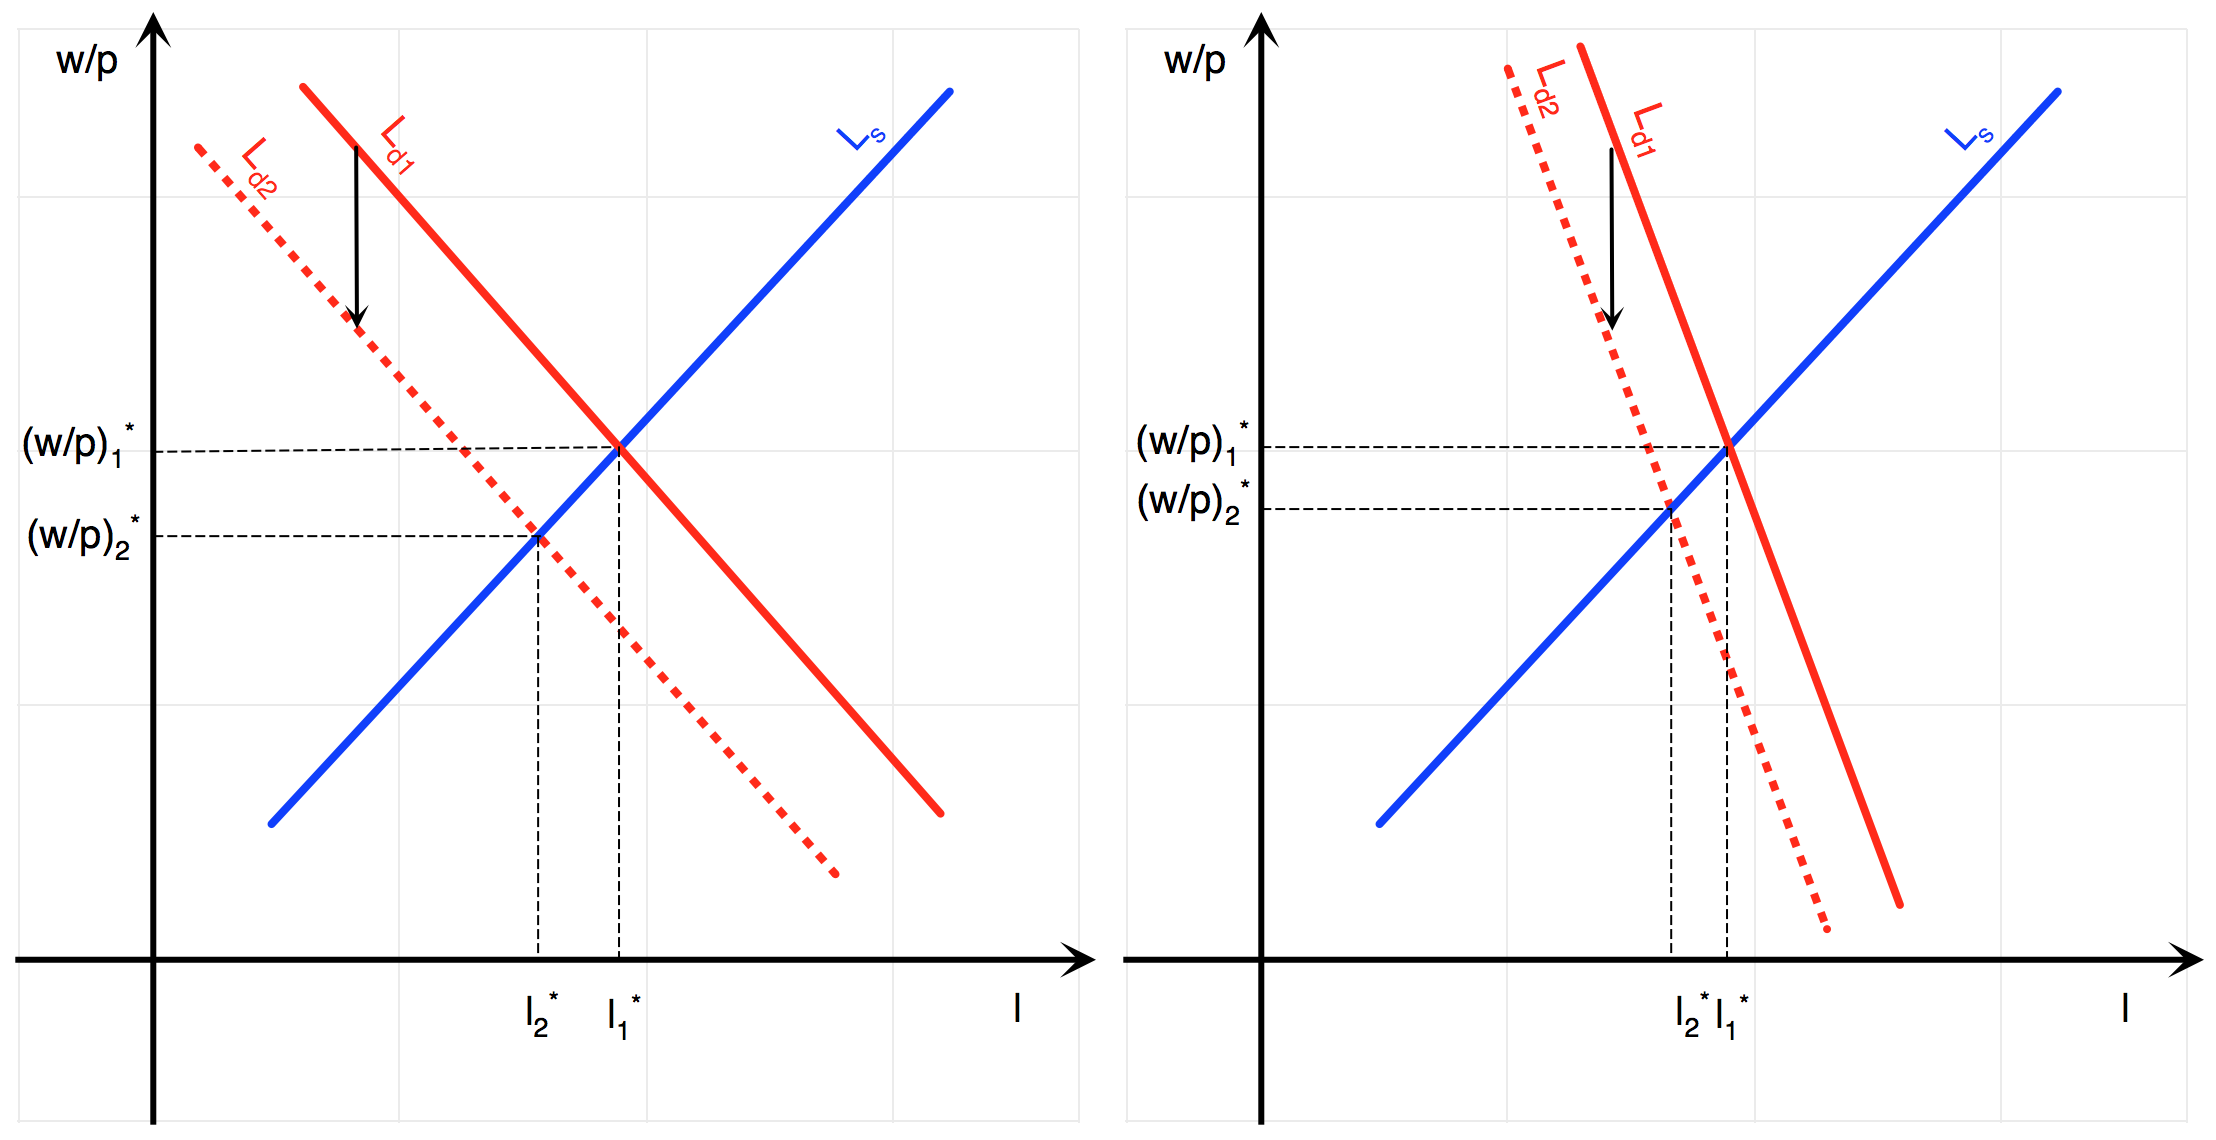
\includegraphics[width=1\linewidth]{graphsketcher/labor-market-productivity-shock-merged} 

}

\caption{\textsc{Labor Market: Productivity Shock}.}\label{fig:labor-market-prod-shock}
\end{figure}

\begin{enumerate}
\def\labelenumi{\arabic{enumi}.}
\setcounter{enumi}{7}
\tightlist
\item
  (Warning! if this idea of an increase in leisure attractiveness seems
  a bit peculiar to you, it also seems odd to me. But it has been
  proposed by some economists as an explanation for unemployment, to
  explain why the real wage did not fall that much during the
  recession.) Similar calculations on the
  \href{https://docs.google.com/spreadsheets/d/1h9JJD8K2_IE166gdj78waf0zu4YDY9Rp3r5oiJR_06s/edit?usp=sharing}{spreadsheet}
  and using the same formulas:
  \[\frac{w}{p} = (1-\alpha)^{\frac{\epsilon}{\alpha+\epsilon}}A^{\frac{\epsilon}{\alpha+\epsilon}} B^{\frac{\alpha}{\alpha+\epsilon}}.\]
  The level of employment is:
  \[l= (1-\alpha)^{\frac{1}{\alpha+\epsilon}}A^{\frac{1}{\alpha+\epsilon}} B^{-\frac{1}{\alpha+\epsilon}}\]
  imply that a 10\% increase in \(B\) leads to a reduction in employment
  and an increase in real wages given by:
  \[\log(l_2)-\log(l_1)=-1.79\%, \qquad \log\left(\frac{w}{p}\right)_2-\log\left(\frac{w}{p}\right)_1=0.60\%.\]
  If \(\epsilon\) is higher, then the effect on both employment and real
  wages is smaller in absolute value. Again, this is intuitive: if labor
  supply is steeper to begin with, then a given increase in \(B\) does
  not lead to as much of a shift in the labor supply curve. Thus, the
  move along the labor demand curve towards lower employment and higher
  wages is not as important then. This is shown on the two figures
  below, where the increase in leisure attractiveness is the same across
  the two experiments: on the left-hand side, epsilon is low, while on
  the right hand side, epsilon is high. \emph{Note}: Again, you may play
  around with the
  \href{https://docs.google.com/spreadsheets/d/1h9JJD8K2_IE166gdj78waf0zu4YDY9Rp3r5oiJR_06s/edit?usp=sharing}{spreadsheet}
  to see what happens when parameters are changed.
\end{enumerate}



\begin{figure}

{\centering 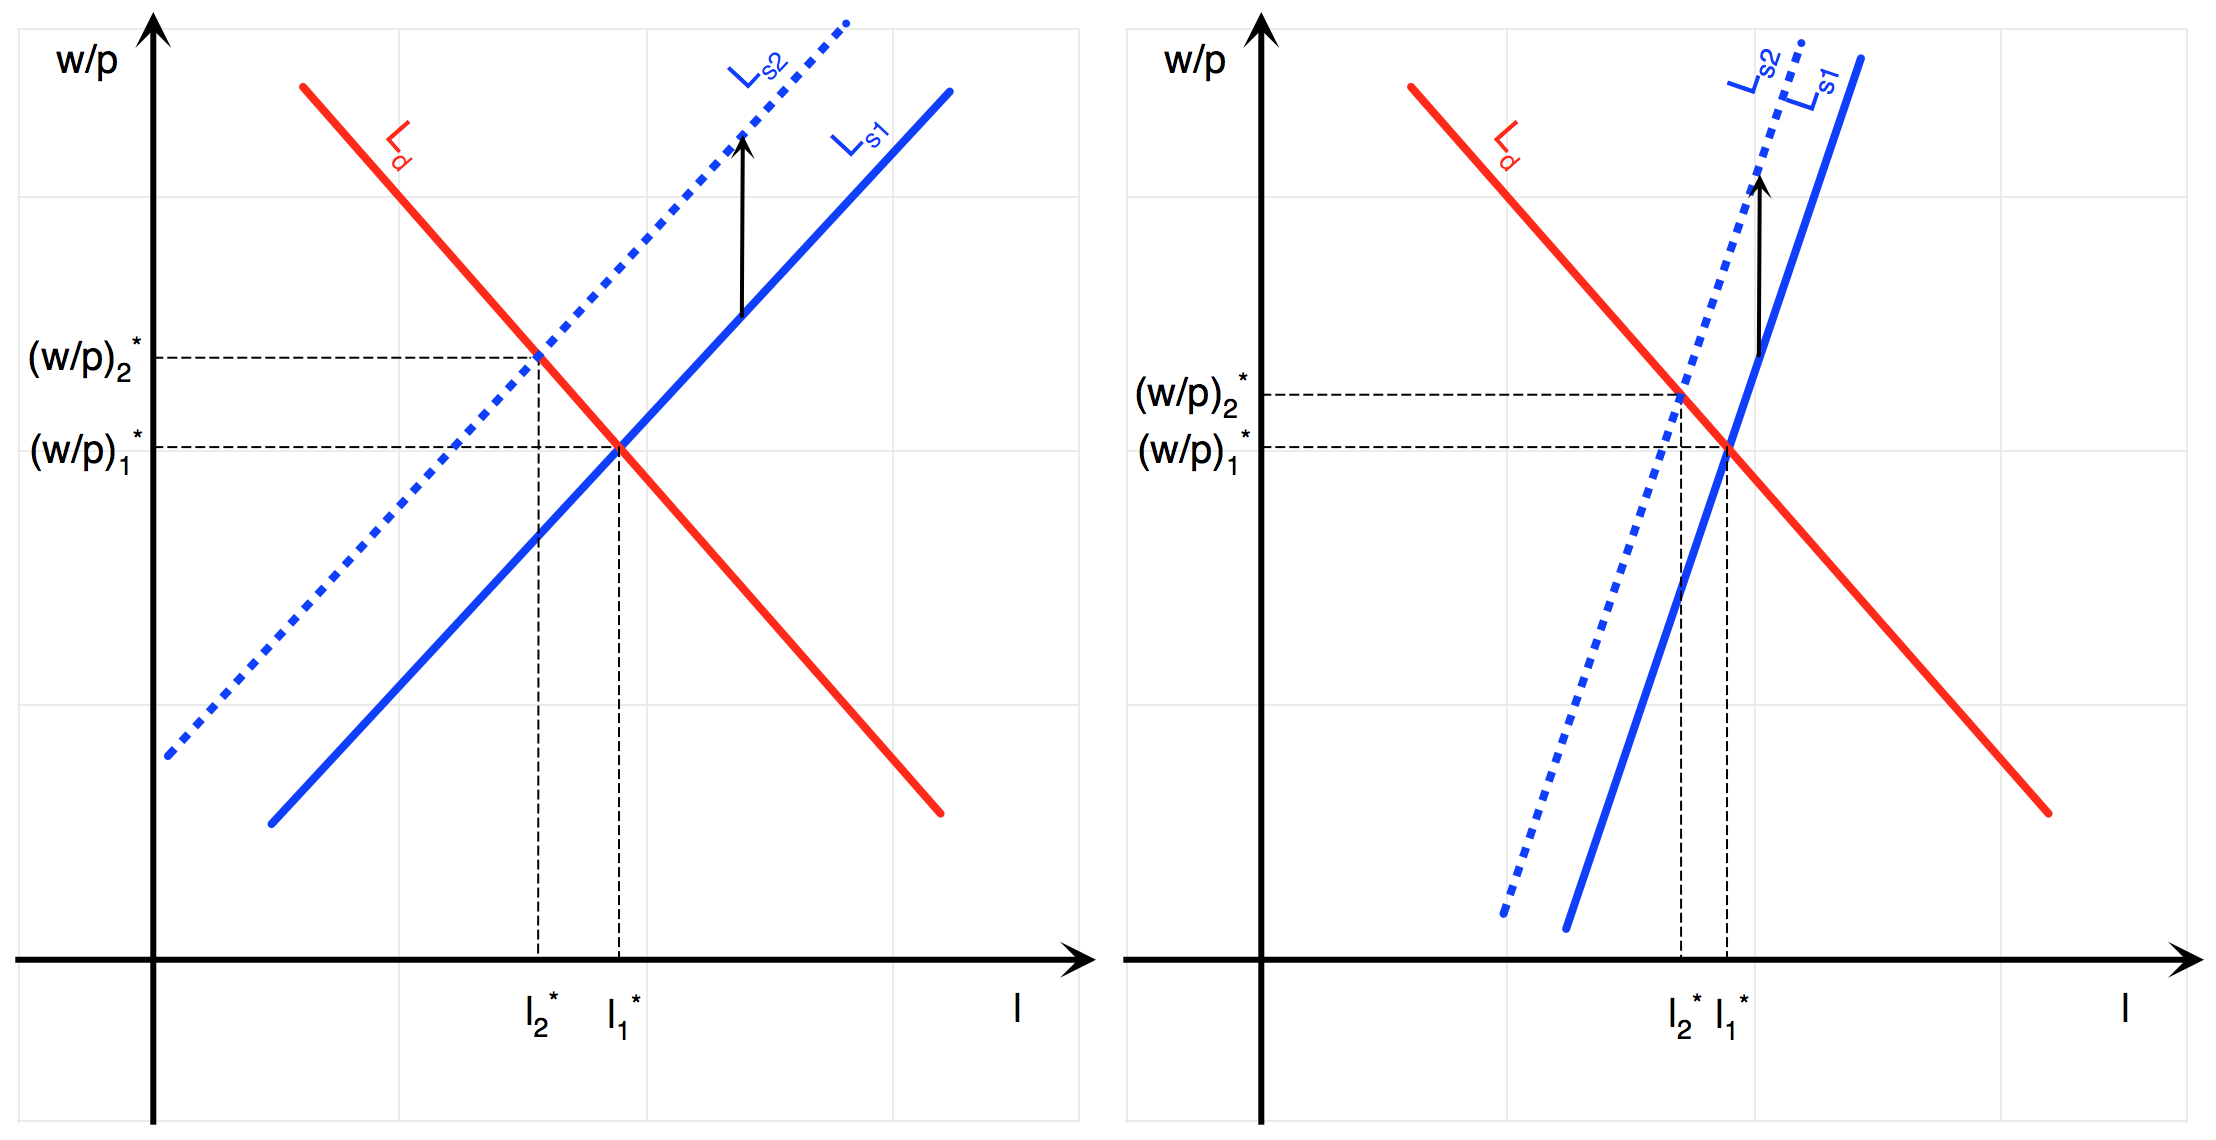
\includegraphics[width=1\linewidth]{graphsketcher/labor-market-laziness-shock-merged} 

}

\caption{\textsc{Labor Market: Laziness Shock}.}\label{fig:labor-market-laziness-shock}
\end{figure}

\section{\texorpdfstring{The ``Keynesian'' Labor Market
Model}{The Keynesian Labor Market Model}}\label{the-keynesian-labor-market-model-1}

\begin{enumerate}
\def\labelenumi{\arabic{enumi}.}
\item
  One way to answer this question is to note that with a fall in
  productivity, the labor demand curve will shift to the left (as in
  \protect\hyperlink{labor-market}{lecture 6}). If real wages are rigid,
  then workers are off their labor supply curve (they would like to work
  more at the current wage) but still on firms' labor demand curve:
  \[\log\left(\frac{w}{p}\right) = \left[\log A + \log(1-\alpha)\right] -\alpha \log(l).\]
  For a given change in \(\Delta \log A\), the change in employment is
  therefore simply given by the previous expression through:
  \[\Delta \log(l)=\frac{\Delta \log A}{\alpha}.\] In contrast, in the
  previous case, with flexible wages, the change in employment following
  a productivity shock was only:
  \[\Delta \log(l) = \frac{\Delta \log A}{\epsilon+\alpha}.\] Given a
  change in productivity of \(5\%\), which goes from \(2\) to \(1.9\),
  or \(\log(1.9)-\log(2)=5.13\%\) in log points, we get a drop of
  \(15.39\%\) in log points in employment:
  \[\log(l_2)-\log(l_1)=-15.39\%.\]
\item
  In question 7 of the previous exercise, we got in contrast a change:
  \[\log(l_2)-\log(l_1)=-0.96\%,\] a much smaller number. The intuition
  was that the wage falling incentivizes employers to hire more workers.
  Here, in contrast, because the wage is ``too high'' and cannot fall by
  definition, employers do not want to hire them.
\item
  We know from \protect\hyperlink{labor-market}{lecture 6} that if
  leisure becomes more attractive, then employment must fall and the
  real wage must rise. We imagine here that wages are sticky upwards.
  Then, people will be off firms' labor demand curves, but on their
  labor supply curves. Thus, it is still true that:
  \[\log\left(\frac{w}{p}\right)=\log B + \epsilon \log(l).\] For a
  given change in \(\Delta \log B\), given that wages are sticky, the
  change in employment is therefore simply given by the previous
  expression through:
  \[\Delta \log(l)=-\frac{\Delta \log B}{\epsilon}.\] In contrast, in
  the previous case, with flexible wages, the change in employment
  following a \(B\) shock was only:
  \[\Delta \log(l) =- \frac{\Delta \log B}{\epsilon+\alpha}.\] Given an
  increase in \(B\) of \(10\%\), which goes from \(2\) to \(2.2\), or
  \(\log(2.2)-\log(2)=9.53\%\) in log points, we get a drop of
  \(1.91\%\) in log points in employment:
  \[\log(l_2)-\log(l_1)=-1.91\%.\]
\item
  In question 8 of the previous exercise, we got in contrast a change:
  \[\log(l_2)-\log(l_1)=-1.79\%,\] a somewhat smaller number. The
  intuition was that the wage increasing would have incentivized workers
  to work more. But because wages are sticky, this did not happen.
\end{enumerate}

\section{The Bathtub model}\label{the-bathtub-model-1}

Assume a monthly job separation rate equal to \(s=1\)\%, and a monthly
job finding rate equal to \(f=20\)\%. Assume that the labor force is
given by \(L=159\) million.

\begin{enumerate}
\def\labelenumi{\arabic{enumi}.}
\item
  The steady state unemployment rate is obtained by equating separations
  and job findings in the steady state, so that: \[
  \begin{aligned}
  &s E^{*} = f U^{*} \quad \Rightarrow \quad sL - s U^{*} = fU^{*}\\
  &\quad \Rightarrow \quad U^{*}=\frac{s}{s+f}L \quad \Rightarrow \quad u^{*}=\frac{s}{s+f}.
  \end{aligned}
  \] The steady state unemployment rate \(u^{*}\), number of people
  unemployed \(U^{*}\), and number of people losing or finding a job
  each month, are given by (see the
  \href{https://docs.google.com/spreadsheets/d/1h9JJD8K2_IE166gdj78waf0zu4YDY9Rp3r5oiJR_06s/edit?usp=sharing}{spreadsheet}):
  \[u^{*}=4.76\%, \quad U^{*}=7,571,429, \quad f U^{*} = 1,514,286.\]
\item
  Again, there are many ways we can proceed here. One is to use the
  \href{https://docs.google.com/spreadsheets/d/1h9JJD8K2_IE166gdj78waf0zu4YDY9Rp3r5oiJR_06s/edit?usp=sharing}{spreadsheet}
  to iterate on the law of motion, that is calculate \(u_{t+1}\) as a
  function of \(u_t\) and then see graphically when the given
  unemployment rate is reached. The law of motion is:
  \[U_{t+1}-U_t = s(L-U_t) -f U_t.\] Thus (see
  \protect\hyperlink{labor-market}{lecture 6}):
  \[U_{t+1}=sL + \left(1-s-f\right)U_t.\] Dividing both sides by \(L\),
  and denoting by \(u_{t}=U_t/L\) the \emph{rate} of unemployment:
  \[u_{t+1}=s+\left(1-s-f\right)u_t.\] We find that the unemployment
  rate reaches 5\% after approximately \textbf{11 months} (the unit of
  time is one month). A second method is to do a bit of algebra before
  using the computer. We write the law of motion for unemployment
  (again, see \protect\hyperlink{labor-market}{lecture 6} for details):
  \[\begin{aligned}
  &U_{t+1}-U_t = s(L-U_t) -f U_t \\
  & \quad \Rightarrow \quad U_{t}-U^{*}=(1-s-f)^t\left(U_0-U^{*}\right).
  \end{aligned}\] Dividing everything by \(L\) gives everything in terms
  of unemployment \emph{rates}:
  \[u_{t}=(1-s-f)^t\left(u_0-u^{*}\right) + u^{*}.\] Thus, starting from
  an unemployment rate \(u_0\) it is possible to get a value for all
  subsequent \(u_t\), using the above formula. We may then use the
  \href{https://docs.google.com/spreadsheets/d/1h9JJD8K2_IE166gdj78waf0zu4YDY9Rp3r5oiJR_06s/edit?usp=sharing}{spreadsheet}
  to compute this and find that the unemployment rate reaches 5\% after
  approximately. Again find that the unemployment rate reaches 5\% after
  approximately \textbf{11 months} (the unit of time is one month). A
  third method is to in fact do all the algebra and calculate the time
  \(T\) we are looking for explicitely. We are looking for \(T\) such
  that \(u_t \leq \bar{u}=5\%\) for \(t \geq T\). This implies: \[
  \begin{aligned}
  &(1-s-f)^t\left(u_0-u^{*}\right) + u^{*} \leq \bar{u}\\
  &\quad \Rightarrow \quad (1-s-f)^t \leq \frac{\bar{u}-u^{*}}{u_0 - u^{*}} \\
  & \quad \Rightarrow \quad t  \log(1-s-f) \leq \log\frac{\bar{u}-u^{*}}{u_0 - u^{*}} \\
  & \quad \Rightarrow \quad t   \geq \frac{\log\frac{\bar{u}-u^{*}}{u_0 - u^{*}}}{\log(1-s-f)}.
  \end{aligned}
  \] (be careful, \(\log(1-s-f)\) is negative because \(1-s-f\) is lower
  than \(1\) so you have to change the inequality from \(\leq\) to
  \(\geq\)). A numerical application using the
  \href{https://docs.google.com/spreadsheets/d/1h9JJD8K2_IE166gdj78waf0zu4YDY9Rp3r5oiJR_06s/edit?usp=sharing}{spreadsheet}
  shows that this condition means: \[t \geq 11.07.\] The advantage of
  this method is we know exactly when the unemployment rate reaches 5\%.
  After 11.07 months ! (given the simplicity of the model, displaying
  the second digit does not make much sense, though)
\item
  We are looking for \(f\) such that:
  \[u^{*}=\frac{s}{s+f}\quad \Rightarrow \quad f=\frac{s}{u^{*}}-s,\]
  which implies using these numbers that: \[f=40\%.\] This is intuitive:
  you have double the separation rate, you want double the job finding
  rate for the unemployment rate to be the same in the steady-state.
  Indeed, in the steady state: \[s E^{*}=f U^{*}.\] Therefore, if the
  unemployment rate is the same, then if \(s\) doubles \(f\) must double
  as well.
\item
  See question 2. The
  \href{https://docs.google.com/spreadsheets/d/1h9JJD8K2_IE166gdj78waf0zu4YDY9Rp3r5oiJR_06s/edit?usp=sharing}{spreadsheet}
  should give all the answers. We find: \[t \geq 4.79.\] Thus, the
  unemployment rate reaches 5\% after approximately 5 months.
\item
  The answer is very much contained in questions 2 and 4. If the rates
  of job separations and job finding are higher like they typically are
  in America, the unemployment rate reaches its steady-state value
  faster. This may explain why the United States are able to recover
  faster from shocks than, say, Spain or Italy (at least in terms of
  unemployment rates). Here is some supporting evidence that the
  unemployment rate is more persistent in Europe than in America:\\
  \url{https://db.nomics.world/OECD/EO/USA.UNR.Q}\\
  \url{https://db.nomics.world/OECD/EO/ESP.UNR.Q}\\
  \url{https://db.nomics.world/OECD/EO/ITA.UNR.Q}
\end{enumerate}

\hypertarget{pset5-sol}{\chapter{Problem Set 5 -
Solution}\label{pset5-sol}}

\section{Gregory N. Mankiw - NYT - Nov 30,
2008}\label{gregory-n.-mankiw---nyt---nov-30-2008-1}

\begin{enumerate}
\def\labelenumi{\arabic{enumi}.}
\item
  According to Gregory N. Mankiw, the factors contributing to hold back
  consumption are low consumer confidence and ``wait and see'' behavior
  caused by falling house price values, shrinking 401(k) balances (due
  to the fall of the stock market, my addition) and increased
  unemployment. Yes, these factors can be interpreted in terms of a fall
  in \(c_0\), since they reduce consumption for a given level of income
  \(Y\).
\item
  Gregory N. Mankiw writes: ``Keynesian theory suggests a''paradox of
  thrift." If all households try to save more, a short-run result could
  be lower aggregate demand and thus lower national income. Reduced
  incomes, in turn, could prevent households from reaching their new
  saving goals." This is exactly the type of phenomenon which we
  explained in \protect\hyperlink{paradox-thrift}{lecture 8}: if there
  is a fall in \(c_0\), then output falls and saving falls as a result.
  Because investment is fixed and equal to \(\bar{I}\), output decreases
  until saving equals investment again.
\item
  The neoclassical comment of the article is: ``In normal times, a fall
  in consumption could be met by an increase in investment, which
  includes spending by businesses on plant and equipment and by
  households on new homes.'' This is the usual logic of the Solow (1956)
  model, for instance. What happens in this model is that saving in fact
  determines investment entirely. The way this happens through market
  mechanisms is that the interest rate falls to equate demand and supply
  of capital. The cost of capital falls down to the point where firms
  and households want to invest enough to make productive use of all
  this saving. This logic is somewhat contradictory with the ``paradox
  of thrift'' logic, according to which investment is fixed or even
  increasing with demand (and the interest rate does not clear markets).
\item
  Gregory N. Mankiw is very concerned about ``the long-term fiscal
  picture. Increased government spending may be a good short-run fix,
  but it would add to the budget deficit. The baby boomers are now
  starting to retire and claim Social Security and Medicare benefits.
  Any increase in the national debt will make fulfilling those unfunded
  promises harder in coming years.'' We will talk about this potential
  issue during \protect\hyperlink{public-debt}{lecture 10}.
\end{enumerate}

\section{Procyclical Government
Spending}\label{procyclical-government-spending-1}

\begin{enumerate}
\def\labelenumi{\arabic{enumi}.}
\item
  We write that Output = Demand: \[
  \begin{aligned}
  Y=Z &=C+\bar{I}+G\\
  Y   &=c_{0}+c_{1}\left(Y-T\right)+ \bar{I} + g_{0}+g_{1}Y\\
  Y   &=\left(c_{0}-c_{1}T+g_{0}+\bar{I}\right)+\left(c_{1}+g_{1}\right)Y \\
  & \Rightarrow \quad \boxed{Y=\frac{1}{1-c_{1}-g_{1}}\left(c_{0}-c_{1}T+g_{0}+\bar{I}\right)}.
  \end{aligned}
  \]
\item
  The tax multiplier is found by computing the change \(\Delta Y\) in
  output corresponding to a given change \(\Delta T\) in taxes: \[
  \begin{aligned}
  \Delta Y = -\frac{c_1}{1-c_1-g_1}\Delta T
  \end{aligned}
  \] Therefore, if \(\Delta T = -\$ 1\), the change in output is
  \(\frac{c_1}{1-c_1-g_1}\). Therefore: \[
  \begin{aligned}
  \boxed{\text{Tax Multiplier} = \frac{c_1}{1-c_1-g_1}}.
  \end{aligned}
  \] The multiplier is higher in this economy than when government
  spending does not depend on GDP since: \[
  \begin{aligned}
  \frac{c_1}{1-c_1-g_1}>\frac{c_1}{1-c_1}.
  \end{aligned}
  \] The intuition is that government spending automatically increases
  when GDP increases, which increases demand further. Thus, the
  multiplier is higher.
\item
  This policy appears to be the opposite of what automatic stabilizers
  are doing, which is to stabilize the economy. The government is having
  a very procyclical policy, which means that when things go well, it is
  spending more and therefore helping things go even better; while when
  things go wrong, it is making it worse by cutting spending. This is
  clearly not a good policy ! Note however that this is the policy you
  end up having if you follow a fixed deficit rule, for instance. With a
  fixed deficit rule, \(T-G\) needs to be constant. If \(T\) depend on
  GDP through automatic stabilizers, through \(T=t_0+t_1 Y\) then by
  construction \(G\) needs to respond as well, and it needs to be that
  \(g_1 = t_1\).
\item
  The (ZZ) curve in this problem has a slope equal to \(c_1+g_1\). The
  impulse to autonomous spending is given by \(\$ c_1\), since one
  dollar of decreased taxes leads to an increase in consumption equal
  \(c_1\). This increase leads to a second round of increased
  consumption and investment \(c_1(c_1+g_1)\), and so on: \[
  \begin{aligned}
  \text{Tax Multiplier} &= c_1 + c_1(c_1+g_1) + c_1(c_1+g_1)^2 + ... + c_1(c_1+g_1)^n + ...\\
  &= c_1\left(1 + (c_1+g_1) + (c_1+g_1)^2 + ... + (c_1+g_1)^n + ...\right) \\
  \text{Tax Multiplier} &=c_1 \sum_{i=0}^{+\infty}(c_1+g_1)^i =  \frac{c_1}{1-c_1-g_1}
  \end{aligned}
  \] A graphical justification for the multiplier is given below. The
  initial impulse is given by \(c_1\). A fraction \(c_1+g_1\) of the
  additional income injected in the economy is being consumed, so that
  adds \(c_1(c_1+g_1)\). This repeats itself in a loop, and all of these
  effects are summed up, so that the total effect is:
  \[c_1 + c_1(c_1+g_1)\]
\end{enumerate}




\begin{figure}

{\centering 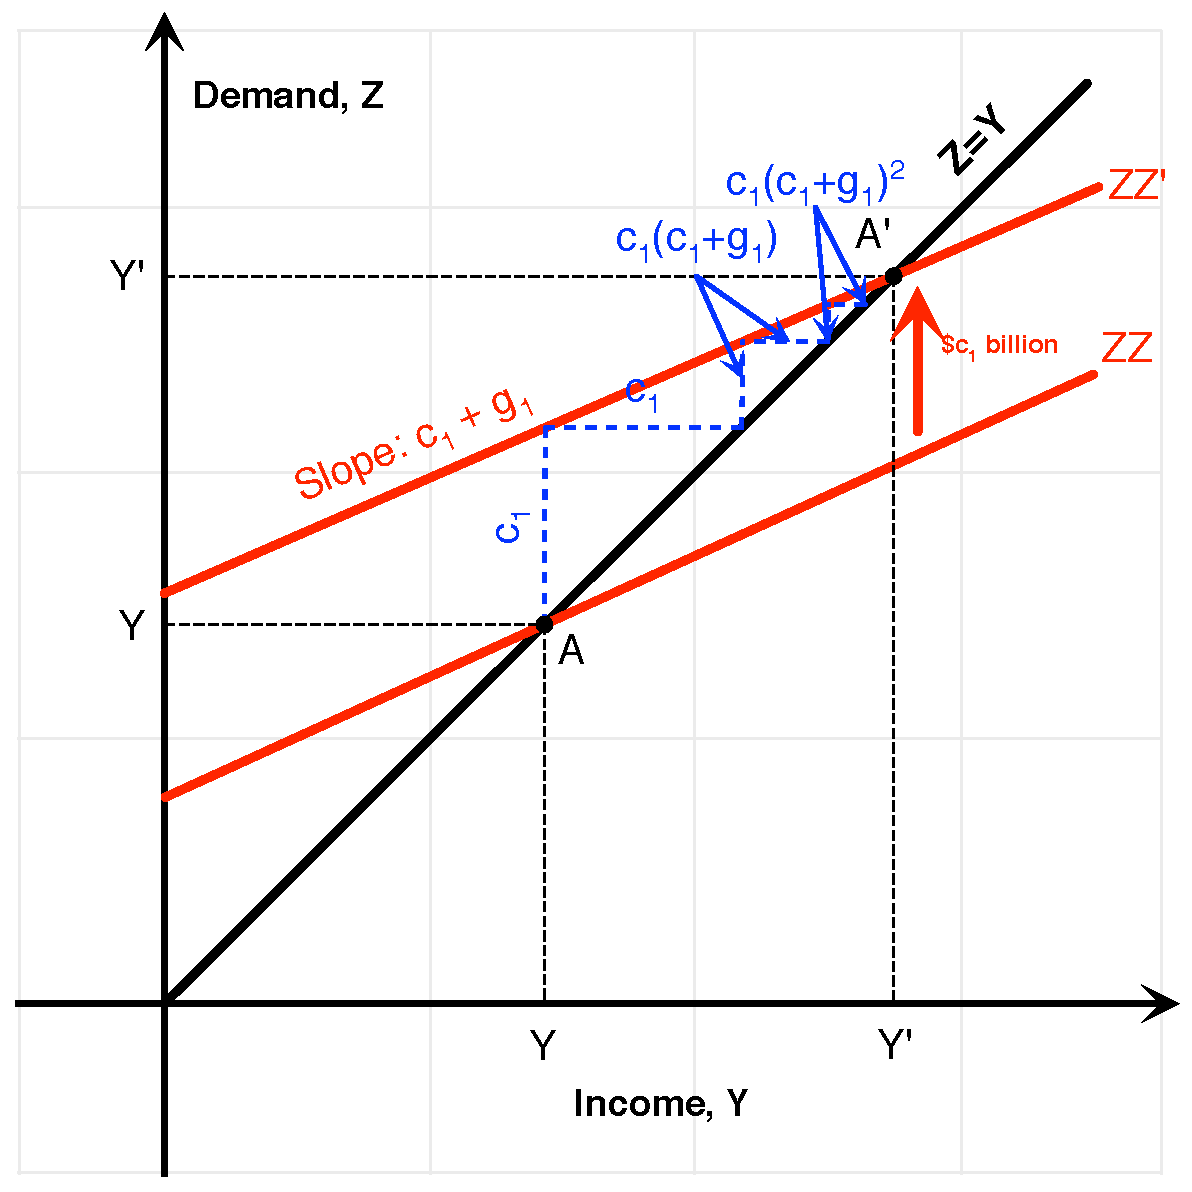
\includegraphics[width=0.6\linewidth]{graphsketcher/midterm} 

}

\caption{\textsc{Graphical Interpretation for the
Multiplier}.}\label{fig:graphical-multiplier}
\end{figure}

\begin{enumerate}
\def\labelenumi{\arabic{enumi}.}
\setcounter{enumi}{4}
\tightlist
\item
  If \(g_1+c_1>1\), then each new round of spending leads to an even
  greater new round of new income and new spending. Therefore, the above
  infinite sum is then infinite, and the tax multiplier is infinite: \[
  \begin{aligned}
  \text{Tax Multiplier} =c_1 \sum_{i=0}^{+\infty}(c_1+g_1)^i = +\infty.
  \end{aligned}
  \] Of course, this is not possible. Therefore, this just means that
  output cannot be demand-determined and that it is always constrained
  by supply (the amount of inputs there is in the economy).
\end{enumerate}

\section{Accelerator and Automatic
Stabilizer}\label{accelerator-and-automatic-stabilizer-1}

\begin{enumerate}
\def\labelenumi{\arabic{enumi}.}
\item
  We have both an automatic stabilizer as well as an accelerator effect
  of investment. We write, again, the total demand for goods \(Z\) and
  then equate demand to output so that \(Y=Z\): \[
  \begin{aligned}
  Y=Z &=C+\bar{I}+G\\
  Y   &=c_{0}+c_{1} Y - c_1 t_0 - c_1 t_1 Y+ b_0+ b_{1}Y + G\\
  Y   &=\left(c_{0}-c_{1}t_0+b_{0}+G\right)+\left(c_{1}(1-t_1)+b_1\right)Y \\
  & \Rightarrow \quad \boxed{Y=\frac{1}{1-b_{1}-c_{1}(1-t_1)}\left(c_{0}-c_{1}t_0+b_{0}+G\right)}.
  \end{aligned}
  \]
\item
  The condition is now given by: \[b_1 + c_1(1-t_1)<1.\]
\item
  If this condition isn't satisfied, then the multiplier becomes
  infinite: one dollar of stimulus leads to more than 1 dollar in
  additional spending, etc. This leads to an infinite sum. This does
  not, of course, mean that GDP becomes infinite. It just means that
  output cannot be constrained by demand, and that the Keynesian model
  no longer applies. Such an economy should always be neoclassical, in
  other words GDP should always be limited by available factors of
  production (capital and labor).
\item
  The graph is very similar to the usual one, only that the slope is
  \(b_1+c_1(1-t_1)\). (if asked for it in an exam, you need to provide
  it) The geometric sum is:
  \[1+ \left(b_1+c_1(1-t_1)\right) + \left(b_1+c_1(1-t_1)\right)^2 + ... = \frac{1}{1-b_1-c_1(1-t_1)}.\]
  (again, you will need to provide the multiplier intuition when asked
  for it in an exam)
\end{enumerate}

\hypertarget{pset6-sol}{\chapter{Problem Set 6 -
Solution}\label{pset6-sol}}

\section{Another Numerical Example}\label{another-numerical-example-1}

\begin{enumerate}
\def\labelenumi{\arabic{enumi}.}
\item
  For a household, the threshold to be in the top 1\% is around
  \textbf{\$421,926} according to the Economic Policy Institute. Let me
  Google that for you: \url{http://bfy.tw/KhF4}.
\item
  Using the given notations (and those of
  \protect\hyperlink{redistributive}{lecture 9}), total income is the
  sum of the top 1\% income and that of the bottom 99\%:
  \[Y=\lambda N \underline{y}+(1-\lambda) N \bar{y}.\] Since
  \(\bar{y}=\gamma \underline{y}\) we have:
  \[Y=\lambda N \underline{y}+(1-\lambda) N \gamma \underline{y}.\] The
  total income for the bottom 99\% \(\underline{Y}\) is given by:
  \[\underline{Y}=\lambda N \underline{y}.\] Therefore, the share of
  total income captured by the bottom 99\% is: \[
  \begin{aligned}
  \frac{\underline{Y}}{Y}&=\frac{\lambda N \underline{y}}{\lambda N \underline{y}+(1-\lambda) N \gamma \underline{y}}\\
  \frac{\underline{Y}}{Y}&=\frac{\lambda}{\lambda +(1-\lambda) \gamma}
  \end{aligned}
  \] Denoting by \(\nu\) the share of income going to the low income: \[
  \begin{aligned}
  \nu &\equiv \frac{\underline{Y}}{Y}\\
  \nu &=\frac{\lambda}{\lambda +(1-\lambda) \gamma}
  \end{aligned}
  \] Solving for \(\gamma\): \[
  \begin{aligned}
  & \frac{\lambda}{\lambda +(1-\lambda) \gamma} = \nu \quad \Rightarrow \quad  \lambda  = \lambda \cdot\nu + (1-\lambda)\gamma \cdot \nu \\
  & \quad \Rightarrow \quad \lambda \cdot (1-\nu)=\gamma \cdot (1-\lambda) \cdot \nu \quad \Rightarrow \quad \boxed{\gamma = \frac{\lambda}{1-\lambda}\frac{1-\nu}{\nu}}
  \end{aligned}
  \] A numerical application is \(\nu=0.8\) and \(\lambda = 0.99\) so
  that: \[
  \begin{aligned}
  \gamma &= \frac{0.99}{1-0.99}\frac{1-0.8}{0.8}\\
   &= \frac{99}{4} \\
  \gamma &= 24.75
  \end{aligned}
  \] This implies that on average, high income earners in the top 1\%
  are approximately \textbf{25 times richer} (exactly 24.75 times
  richer) than low income earners in the bottom 99\% (note that you can
  use the above formula to recover the \(\gamma = 9\) from the class,
  using \(\lambda = 0.9\) and \(\nu = 0.5\) since
  \(\gamma = 0.9/0.1 \cdot0.5/0.5 = 9\)).
\item
  Total consumption by the low income earners \(\underline{C}\) is such
  that: \[
  \begin{aligned}
  \underline{C}&=\lambda N \underline{c}\\
  &=\lambda N \left(\underline{c}_{0}+\underline{c}_{1}(\underline{y}-\underline{t})\right)\\
  &=\lambda N  \underline{c}_{0} + \lambda N  (1-t_1) \underline{c}_{1}\underline{y}-\lambda N  \underline{c}_{1} \underline{t}_0\\
  \underline{C}&=\left[\lambda N  \underline{c}_{0}-\lambda  N \underline{c}_{1} \underline{t}_0 \right]+ \frac{\lambda \underline{c}_{1}}{\lambda+(1-\lambda)\gamma}(1-t_1)Y
  \end{aligned}
  \] Symmetrically, consumption by the high income earners \(\bar{C}\)
  is such that: \[
  \begin{aligned}
  \bar{C}&=(1-\lambda) N \bar{c}\\
  &=(1-\lambda) N \left(\bar{c}_{0}+\bar{c}_{1}(\bar{y}-\bar{t})\right)\\
  &=(1-\lambda) N  \bar{c}_{0} + (1-\lambda) N (1-t_1) \bar{c}_{1}\bar{y}-(1-\lambda) N  \bar{c}_{1} \bar{t}_0\\
  \bar{C}&=\left[(1-\lambda) N  \bar{c}_{0}-(1-\lambda) N  \bar{c}_{1} \bar{t}_0\right] + \frac{(1-\lambda) \gamma\bar{c}_{1}}{\lambda+(1-\lambda)\gamma}(1-t_1)Y
  \end{aligned}
  \] Therefore, aggregate consumption \(C=\underline{C} + \bar{C}\) is
  given by: \[
  \begin{aligned}
  C&=\underline{C} + \bar{C}\\
  &=\left[\lambda N  \underline{c}_{0}-\lambda  N \underline{c}_{1} \underline{t}_0 \right]+ \frac{\lambda \underline{c}_{1}}{\lambda+(1-\lambda)\gamma}(1-t_1)Y + 
  \left[(1-\lambda)  N \bar{c}_{0}-(1-\lambda) N  \bar{c}_{1} \bar{t}_0\right] + 
  \frac{(1-\lambda) \gamma\bar{c}_{1}}{\lambda+(1-\lambda)\gamma}(1-t_1)Y\\
  &=\left(\lambda N  \underline{c}_{0}+(1-\lambda) N  \bar{c}_{0}\right)-\left(\lambda  N \underline{c}_{1} \underline{t}_0 +(1-\lambda) N  \bar{c}_{1} \bar{t}_0\right) +\frac{\lambda\underline{c}_{1}+\left(1-\lambda\right)\gamma\bar{c}_{1}}{\lambda+(1-\lambda)\gamma}(1-t_1)Y\\
  &=\left[\lambda N  \underline{c}_{0}+(1-\lambda) N  \bar{c}_{0}\right]-\left[\underline{c}_{1} (\lambda  N \underline{t}_0) + \bar{c}_{1} ((1-\lambda) N \bar{t}_0)\right] +\frac{\lambda\underline{c}_{1}+\left(1-\lambda\right)\gamma\bar{c}_{1}}{\lambda+(1-\lambda)\gamma}(1-t_1)Y\\
  C&=C_0 -\left(\underline{c}_{1}\underline{T}_0+\bar{c}_{1}\bar{T}_0\right)+c_1 (1-t_1) Y.
  \end{aligned}
  \] where we have used the suggested notations: \[
  \begin{aligned}
  C_{0}& \equiv \lambda  N \underline{c}_0 + (1-\lambda) N \bar{c}_0\\
  \underline{T}_{0}& \equiv \lambda  N \underline{t}_0\\
  \bar{T}_0 & \equiv (1-\lambda) N \bar{t}_0\\
  c_{1}&\equiv\frac{\lambda\underline{c}_{1}+\left(1-\lambda\right)\gamma\bar{c}_{1}}{\lambda+(1-\lambda)\gamma}.
  \end{aligned}
  \] Therefore, aggregate consumption is given by:
  \[\boxed{C=C_0 -\left(\underline{c}_{1}\underline{T}_0+\bar{c}_{1}\bar{T}_0\right)+c_1 (1-t_1) Y}.\]
\item
  \(c_1\) is the average marginal propensity to consume, where the
  marginal propensity to consume of each group \(\underline{c}_1\) and
  \(\bar{c}_1\) is weighted by their share of income in the population
  \(\underline{Y}/Y\) and \(\bar{Y}/Y\): \[
  \begin{aligned}
  c_1&=\frac{\lambda\underline{c}_{1}+\left(1-\lambda\right)\gamma \bar{c}_{1}}{\lambda+(1-\lambda)\gamma}\\
  &=\frac{\lambda}{\lambda + (1-\lambda)\gamma}\underline{c}_{1} +\frac{(1-\lambda)\gamma}{\lambda+(1-\lambda)\gamma}\bar{c}_{1}\\
  c_1&=\frac{\underline{Y}}{Y}\underline{c}_{1} + \frac{\bar{Y}}{Y}\bar{c}_{1}
  \end{aligned}
  \] This has a straightforward economic interpretation: for each
  additional dollar of output, a fraction \(\underline{Y}/Y\) goes to
  low income earners who consume a fraction \(\underline{c}_1\), and a
  fraction \(\bar{Y}/Y\) goes to high income earners who consume a
  fraction \(\bar{c}_1\). The average propensity to consume is the sum
  of these two fractions. We can then simply compute the average
  marginal propensity to consume when \(\underline{c}_1=1\) and
  \(\bar{c}_1=1/4\): \[
  \begin{aligned}
  c_1 &= \frac{\underline{Y}}{Y}\underline{c}_{1} + \frac{\bar{Y}}{Y}\bar{c}_{1}\\
  &=\frac{4}{5}\cdot 1 + \frac{1}{5}\cdot \frac{1}{4}\\
  c_1 &= \frac{17}{20}
  \end{aligned}
  \] Therefore the average propensity to consume is:
  \[\boxed{c_1 = 0.85}.\]
\item
  Using the expression for aggregate consumption \(C\) in question 3.,
  and that \(I=b_0+b_1 Y\), and plugging it into total aggregate demand
  \(Z\) yields: \[
  \begin{aligned}
  Z   &=C+I+G\\
  &=C_0 -\left(\underline{c}_{1}\underline{T}_0+\bar{c}_{1}\bar{T}_0\right)+c_1 (1-t_1) Y + b_{0}+b_{1}Y+G\\
  Z   &=\left[C_0 -\left(\underline{c}_{1}\underline{T}_0+\bar{c}_{1}\bar{T}_0\right)+ b_{0} + G \right]+ \left(c_1(1-t_1) + b_1\right) Y 
  \end{aligned}
  \] Equating aggregate demand to aggregate income \(Z = Y\) gives the
  value for output (see the lecture notes for details):
  \[\boxed{Y=\frac{1}{1-\left(1-t_{1}\right)c_{1}-b_{1}}\left[C_0-\underline{c}_{1}\underline{T}_{0}-\bar{c}_{1}\bar{T}_{0}+b_{0}+G\right]}\]
\item
  As in \protect\hyperlink{redistributive}{lecture 9}, a 100 billion
  dollars tax cut on the top 1\% \(\Delta \bar{T}_0 = -100\) leads to an
  increase in GDP given by: \[
  \begin{aligned}
  \Delta Y &=\frac{-\bar{c}_1 \Delta \bar{T}_0}{1-c_1(1-t_1)-b_1}\\
  &=\frac{-1/4 * (-100 \text{ billion})}{1-0.85 \cdot 0.75-1/6}\\
  \Delta Y&\approx 127.6 \text{ billion}.
  \end{aligned}
  \] Thus, according to these numbers, we get a \textbf{127.6 billion
  dollars} increase in GDP. The impact on the government surplus is
  given by: \[
  \begin{aligned}
  \Delta\left(T-G\right)&=\Delta T\\
  &=\Delta\bar{T}_{0}+\Delta\underline{T}_{0}+t_1\Delta Y\\
  &=\Delta\bar{T}_{0}+t_1\Delta Y \\
  & \approx -100 + \frac{1}{4} \cdot 127.6\\
  \Delta\left(T-G\right)  & \approx-68.1 \text{ billion}
  \end{aligned}
  \] Thus, we get a \textbf{68.1 billion dollars} increase in the
  government deficit.
\item
  A 100 billion dollars tax cut on the bottom 99\%
  \(\Delta \underline{T}_0 = -100\) leads to an increase in GDP given
  by: \[
  \begin{aligned}
  \Delta Y &=\frac{-\underline{c}_1 \Delta \underline{T}_0}{1-c_1(1-t_1)-b_1}\\
  &=\frac{-1 * (-100 \text{ billion})}{1-0.85 \cdot 0.75-1/6}\\
  \Delta Y&\approx 510.6 \text{ billion}.
  \end{aligned}
  \] Thus, according to these numbers, we get a \textbf{510.6 billion
  dollars} increase in GDP. The impact on the government surplus is
  given by: \[
  \begin{aligned}
  \Delta\left(T-G\right)&=\Delta T\\
  &=\Delta\bar{T}_{0}+\Delta\underline{T}_{0}+t_1\Delta Y\\
  &=\Delta\underline{T}_{0}+t_1\Delta Y \\
  & \approx -100 + \frac{1}{4} \cdot 510.6\\
  \Delta\left(T-G\right)  & \approx 27.6 \text{ billion}
  \end{aligned}
  \] Thus, despite the 100 billion dollars tax cut, we get a
  \textbf{27.6 billion dollars} increase in the government surplus, or a
  reduction in the government deficit. In this situation, tax cuts
  \textbf{more than pay for themselves}. This seems like a much better
  policy than the tax reduction on the rich. However, we will see in the
  next lectures that things are not so straightforward.
\item
  Finally, a 100 billion dollars tax cut on the bottom 99\%
  \(\Delta \underline{T}_0 = -100\) financed by a 100 billion tax
  increase on the top 1\% \(\Delta \bar{T}_0 = 100\) leads to an
  increase in GDP given by: \[
  \begin{aligned}
  \Delta Y &=\frac{(\underline{c}_1-\bar{c}_1) \Delta \bar{T}_0}{1-c_1(1-t_1)-b_1}\\
  &=\frac{(1-1/4) * (100 \text{ billion})}{1-0.85 \cdot 0.75-1/6}\\
  \Delta Y&\approx 383.0 \text{ billion}
  \end{aligned}
  \] Thus, according to these numbers, we get a \textbf{383.0 billion
  dollars} increase in GDP. The impact on the government surplus is
  given by: \[
  \begin{aligned}
  \Delta\left(T-G\right)&=\Delta T\\
  &=\Delta\bar{T}_{0}+\Delta\underline{T}_{0}+t_1\Delta Y\\
  &=t_1\Delta Y \\
  &\approx \frac{1}{4} \cdot 383.0\\
  \Delta\left(T-G\right)  & \approx 95.7 \text{ billion}
  \end{aligned}
  \] We get a \textbf{95.7 billion dollars} increase in the government
  surplus, or a reduction in the government deficit.
\item
  If there are no automatic stabilizers (\(t_1 = 0\)), then the
  multiplier apparently becomes infinite since
  \(1-c_1-b_1 = 1-0.85 - 1/6<0\). However, this is impossible, as there
  are only finite resources in the economy. Therefore, this implies that
  output is determined by supply constraints (amount of labor, capital,
  and technology), as in the Solow growth model, and that the Keynesian
  type of analysis no longer applies.\\
  In fact, as I said during the lecture, this result is intuitive. If
  \(1-c_1<b_1\), then this implies that the marginal propensity to
  invest \(b_1\) is higher than the marginal propensity to save
  \(1-c_1\). As a result, we never get to a Keynesian situation of ``too
  much saving''.
\end{enumerate}

\hypertarget{pset7-sol}{\chapter{Problem Set 7 -
Solution}\label{pset7-sol}}

\section{Another overlapping-generations model with government
debt}\label{another-overlapping-generations-model-with-government-debt-1}

\begin{enumerate}
\def\labelenumi{\arabic{enumi}.}
\item
  We could use the expressions derived in
  \protect\hyperlink{two-period}{lecture 3} for a 2-period consumption
  problem, since utility is logarithmic with \(\beta = 2\). However, we
  will instead derive the formulas from scratch, using the same
  techniques we used in that lecture (and so should you during an exam).
  The problem we are looking to solve is the following: \[
  \begin{aligned}
  & \max_{c_t^y, c_{t+1}^o} \quad \log(c_t^y) + 2\log(c_{t+1}^o)\\
  & \quad \text{s.t} \quad c_{t}^{y}+\frac{c_{t+1}^{o}}{1+r_t}=w_{t}.
  \end{aligned}
  \] Again, there are many methods through which we could potentially
  solve this problem. We can just use the ratio os marginal utilities to
  get the optimality condition:
  \[\frac{1/c_t^y}{2/c_{t+1}^o}=1+r_t \quad \Rightarrow \quad c_{t+1}^o = 2(1+r_t)c_t^y.\]
  Plugging back in the intertemporal budget constraint: \[
  \begin{aligned}
  &c_{t}^{y}+\frac{c_{t+1}^{o}}{1+r_t}=w_{t} \quad \Rightarrow \quad c_t^y + 2 c_t^y = w_t\\
  &\quad \Rightarrow \quad \boxed{c_t^y = \frac{w_t}{3}}.
  \end{aligned}
  \] And finally, plugging this in the optimality condition: \[
  \begin{aligned}
  c_{t+1}^o = 2(1+r_t)c_t^y \quad \Rightarrow \quad \boxed{c_{t+1}^o = (1+r_t)\frac{2w_t}{3}}.
  \end{aligned}
  \]
\item
  Saving is given by \(w_t - c_t^y = 2w_t/3\) and depreciation is
  \(\delta = 1\), and therefore the law of motion of the capital stock
  is: \[K_{t+1} - K_t = \frac{2w_t}{3}-K_t.\] From firms' optimality
  condition, the wage is just the marginal product of labor:
  \[w_{t}=\frac{\partial Y_{t}}{\partial L_{t}}=\frac{2}{3}K_{t}^{1/3}L_{t}^{-1/3}=\frac{2}{3}K_{t}^{1/3}.\]
  Therefore, we get finally the following law of motion for capital:
  \[K_{t+1} = \frac{4}{9}K_{t}^{1/3}.\]
\item
  The steady-state capital stock \(K^{*}\) is such that: \[
  \begin{aligned}
  & K^{*} = \frac{4}{9}(K^{*})^{1/3} \quad \Rightarrow \quad (K^{*})^{2/3} = \frac{4}{9}\\
  & \quad \Rightarrow \quad K^{*} = \left(\frac{4}{9}\right)^{3/2} \quad \Rightarrow \quad K^{*} = \left(\frac{2}{3}\right)^{3} \quad \Rightarrow \quad \boxed{K^{*} = \frac{8}{27}}.
  \end{aligned}
  \] The (net) steady-state real interest rate \(r^{*}\) is given by the
  fact that the marginal product of capital is equal to
  \(r^{*} + \delta\), which is \(1+r^{*}\) here: \[
  \begin{aligned}
  1+r^{*} = \frac{1}{3}(K^{*})^{-2/3} \quad \Rightarrow \quad r^{*}=\frac{1}{3}\frac{1}{(K^{*})^{2/3}}-1
  \end{aligned}
  \] Thus, using the above expression that
  \((K^{*})^{2/3} = \frac{4}{9}\), we get:
  \[r^{*}=\frac{1}{3} \cdot \frac{9}{4}-1 \quad \Rightarrow \quad  \boxed{r^{*}= -25\%}\]
  Comment: you may think that this interest rate is counterfactually way
  too low. However, remember that one period is a generation here. (that
  is, the age at which people have a child on average, about 30 years)
  The corresponding annual interest rate is thus:
  \[(1+r^{*})^{1/30}-1 \approx -0.95\%.\] Steady-state output \(Y^{*}\)
  is given by the production function:
  \[Y^{*} = (K^{*})^{1/3} = \left(\frac{8}{27}\right)^{1/3} \quad \Rightarrow \quad \boxed{Y^{*} =\frac{2}{3}}\]
  the steady-state wage \(w^{*}\) is given by the marginal product of
  labor evaluated at the steady-state capital stock:
  \[w^{*}=\frac{2}{3}(K^{*})^{1/3}=\frac{2}{3}Y^{*} \quad \Rightarrow \quad \boxed{w^{*} = \frac{4}{9}}.\]
  The steady-state consumption of the young is:
  \[(c^y)^{*} = \frac{1}{3}w^{*} \quad \Rightarrow \quad \boxed{(c^y)^{*} = \frac{4}{27}}.\]
  The steady-state consumption of the old is:
  \[(c^o)^{*} = (1+r^{*})\frac{2w^{*}}{3} = \frac{3}{4} \cdot \frac{8}{27} = \frac{3}{9} \quad \Rightarrow \quad \boxed{(c^o)^{*} = \frac{2}{9}}\]
\item
  The Golden Rule (net) interest rate \(r^{*}_g\) is given by
  \(r^{*}_g=0\), again because there is no growth. Using this and
  plugging back to get an expression for \((K^{*})_g\): \[
  \begin{aligned}
  1+r^{*}_g = \frac{1}{3}(K^{*}_g)^{-2/3} \quad \Rightarrow \quad K_g^{*}=\frac{1}{3^{3/2}} \quad \Rightarrow \quad \boxed{K_g^{*}=\frac{1}{3\sqrt{3}}}
  \end{aligned}
  \] The Golden Rule output \(Y^{*}_g\) is then given by the production
  function:
  \[Y^{*}_g=(K^{*}_g)^{1/3} = \left(\frac{1}{3^{3/2}}\right)^{1/3} = \frac{1}{3^{1/2}} \quad \Rightarrow \quad \boxed{Y^{*}_g = \frac{1}{\sqrt{3}}}\]
  The Golden Rule wage \(w^{*}_g\) is:
  \[w^{*}_g=\frac{2}{3}(K^{*}_g)^{1/3}=\frac{2}{3}Y^{*}_g \quad \Rightarrow \quad \boxed{w^{*}_g = \frac{2}{3\sqrt{3}}}.\]
  The Golden Rule consumption of the young is:
  \[(c^y)^{*}_g = \frac{1}{3}w^{*}_g \quad \Rightarrow \quad \boxed{(c^y)^{*}_g = \frac{2}{9\sqrt{3}}}.\]
  The Golden Rule consumption of the old is:
  \[(c^o)^{*}_g = \frac{2}{3}w^{*}_g \quad \Rightarrow \quad \boxed{(c^o)^{*}_g = \frac{4}{9\sqrt{3}}}.\]
\item
  We have the following inequalities: \[
  \begin{aligned}
  r^{*}_g &> r^{*}\\
  K^{*}_g &< K^{*}\\
  Y^{*}_g &< Y^{*}\\
  w^{*}_g &< w^{*}\\
  (c^y)^{*}_g &< (c^y)^{*} \quad \text{since} \quad \frac{2}{9\sqrt{3}}<\frac{4}{27} \quad \Leftrightarrow \quad \sqrt{3} <2 \\
  (c^o)^{*}_g &> (c^o)^{*} \quad \text{since} \quad \frac{4}{9\sqrt{3}}>\frac{2}{9} \quad \Leftrightarrow \quad 2 >\sqrt{3} \\
  \end{aligned}
  \] The economic intuition is that the capital stock is at a lower
  steady-state under the Golden-Rule, so that the marginal product of
  capital is lower, output is lower, and the wage is lower. For
  consumption, it is higher when old under the Golden Rule (because the
  return is higher, which more than compensates for the lowest wage) and
  lower when young because the wage is lower. Overall, the Golden-Rule
  steady-state utility is given by:
  \[U^*_g = \log(c^y)^{*}_g+2\log(c^o)^{*}_g = \log\frac{2}{9\sqrt{3}}+2\log \frac{4}{9\sqrt{3}}\]
  While the steady-state utility is:
  \[U^* = \log(c^y)^{*}+2\log(c^o)^{*} = \log\frac{4}{27}+2\log \frac{2}{9}\]
  We compute \(U^{*}_g-U^{*}\) to see which steady-state utility is
  greater: \[
  \begin{aligned}
  U^{*}_g-U^{*} &= \log\frac{2}{9\sqrt{3}}+2\log \frac{4}{9\sqrt{3}} - \log\frac{4}{27}-2\log \frac{2}{9}\\
  &= \log \left[\frac{2}{9\sqrt{3}} \cdot \left(\frac{4}{9\sqrt{3}}\right)^2 \cdot\frac{27}{4} \cdot \left(\frac{9}{2}\right)^2\right]\\
  &=\log \left[\frac{2 \cdot 4^2 \cdot 27 \cdot 9^2}{9\sqrt{3} \cdot 9^2 \cdot 3\cdot 4 \cdot 4}\right]\\
  U^{*}_g-U^{*}&=\log \frac{2}{\sqrt3} > \log \frac{2}{\sqrt4}=\log1 =0
  \end{aligned}
  \] Thus, we conclude that the Golden Rule level of steady-state
  utility is higher than the equilibrium level of steady-state utility
  since:
  \[U^{*}_g-U^{*}>0\quad \Rightarrow \quad \boxed{U^{*}_g>U^{*}}.\] The
  economic intuition for these results is as follows. First, the
  steady-state level of the interest rate was \(r^{*}=-25\) \% - so,
  again, around -1\% per year - which as we know now is below the Golden
  Rule interest rate, which is 0, in an economy which has zero growth in
  the long run. Moreover, we also know that the gross interest rate
  \(R^{*}=1+r^{*}\) is decreasing in the quantity of capital, because of
  decreasing returns to capital. Therefore, if the net interest rate is
  higher at the Golden Rule, then necessarily the capital stock is
  smaller. But if the capital stock is smaller then by virtue of
  \(Y=K^{1/3}\) we know that output is also smaller. For the same
  reason, we know that the wage, which is a fraction \(2/3\) of output,
  is also smaller.
\item
  As in \protect\hyperlink{public-debt}{lecture 10}, we know that the
  level of government debt \(B^{*}_g\) which brings the capital stock to
  the Golden Rule level is that which implies that when savers save
  \(2/3\) of their young age wage, they are able to exactly buy the
  quantity of capital corresponding to the Golden Rule level, as well as
  that public debt. Thus, we get an equation that \(B^{*}_g\) must
  satisfy (note the difference with the lecture notes: this time not all
  the wage is saved, but only a fraction \(2/3\)):
  \[B^{*}_g+K^{*}_g=\frac{2}{3}w^{*}_g\quad\Rightarrow\quad B^{*}_g=\frac{2}{3}w^{*}_g-K^{*}_g.\]
  Substituting: \[
  \begin{aligned}
  B^{*}_g&=\frac{2}{3}w^{*}_g-K^{*}_g\\
  &=\frac{2}{3} \cdot \frac{2}{3\sqrt{3}}-\frac{1}{3\sqrt{3}}\\
  &=\left(\frac{4}{3}-1\right) \cdot \frac{1}{3\sqrt{3}}\\
  B^{*}_g&=\frac{1}{9\sqrt{3}}.
  \end{aligned}
  \] Note that this is considerably less government debt than in the
  lecture notes: this makes sense, as the dynamic inefficiency problem
  is considerably less severe here.
\item
  The lucky generation of retirees is able to consume the sum of what
  that generation would have consumed anyway, since these savings come
  to fruition when they are old, plus what the government gives them:
  \[c_{0}^{o}=\frac{2}{9}+\frac{1}{9\sqrt{3}}=\frac{2\sqrt{3}+1}{9\sqrt{3}}.\]
\item
  Public debt is often criticized as a ``Ponzi scheme'', a negative term
  which is named after Charles Ponzi, who became famous for creating
  this fraudulent system. (although apparently, he was not really the
  first) A \href{https://en.wikipedia.org/wiki/Ponzi_scheme}{Ponzi
  scheme} is a form of fraud, through which a money manager pays very
  big profits to earlier investors (higher than the market interest
  rate), making them think he is a really good investor, while in fact
  he is just able to pay these returns by raising funds from new
  investors. A more recent example is Bernie Madoff (\emph{The Wizard of
  Lies} is an ok HBO movie where
  \href{https://www.youtube.com/watch?v=7JcZ8QFn6U0}{De Niro plays
  Bernie Madoff}). Public debt is also a Ponzi scheme in the overlapping
  generations model, in the sense that the government in fact never
  intends to fully repay all investors: it is always raising new money
  from the young generation, and using this money to reimburse the old
  one. However, this Ponzi scheme is actually good because it solves the
  issue of overaccumulation of capital, and allows everyone to consume
  more.
\item
  If the government puts in place a pay-as-you-go (PAYG) system, giving
  retirees an amount \(B^{*}_g\) each period (where \(B^{*}_g\) is the
  same level of government debt as the one found in question 6), and
  taxing the young an equal amount \(B^{*}_g\), then the money which is
  left for the young to invest in capital is given by
  \(2/3 \cdot w^{*}_g - B^{*}_g\), the income after tax, so that the
  level of capital accumulation is still \(K^{*}_g\). When old, the
  government gives them what they would have gotten from investing in
  government debt had they not been taxes. Therefore, in terms of
  consumption, capital accumulation, everything ``real'', it is exactly
  the same situation. In terms of financial accounting however, the
  young used to have savings on their books (in the form of government
  debt), which they do not have anymore: nothing appears on their bank
  accounts. They have ``implicit assets'' in the sense that the
  government owes them whatever they gave contributed. Symmetrically, it
  does not look like the government has any debt, while it actually has
  ``implicit liabilities'': it owes the young whatever it has been
  taxing them.
\item
  Here, there really is no difference between pay-as-you-go financing
  and deficit financing, except that one appears on the government's
  books (deficit financing), while the other does not (pay-as-you-go
  financing). Pay-as-you-go is thus an implicit government liability:
  instead of having promised to repay creditors, the government has
  promised to repay future retirees who have put money in the system
  when they were working. This helps understand why government debt is
  not a very meaningful statistic: by reclassifying some of its
  liabilities as pension liabilities, the government is able to reduce
  its government debt. A forceful proponent of including pay-as-you-go
  liabilities into government debt numbers is Lawrence Kotlikoff, an
  economist at Boston University. You can read
  \href{https://www.kotlikoff.net/sites/default/files/Kotlikoffbudgetcom2-25-2015.pdf}{here}
  his very dismal assessment of the current U.S. fiscal outlook. As you
  now know, I am not as concerned as he is. As I said during the class,
  what matters really is the value for real interest rates compared to
  growth rates, in order to understand whether this debt can actually be
  rolled over indefinitely or not. Don't hesitate to let me know if you
  feel strongly in the opposite direction, and find my arguments
  unpersuasive !
\end{enumerate}

\hypertarget{pset8-sol}{\chapter{Problem Set 8 -
Solution}\label{pset8-sol}}

\hypertarget{pset9-sol}{\chapter{Problem Set 9 -
Solution}\label{pset9-sol}}

\hypertarget{pset10-sol}{\chapter{Problem Set 10 -
Solution}\label{pset10-sol}}

\bibliography{book.bib,packages.bib}


\end{document}
